% Do not change document class, margins, fonts, etc.
\documentclass[a4paper,oneside,bibliography=totoc]{scrbook}

% some useful packages (add more as needed)
\usepackage[utf8]{inputenc}
\usepackage{graphicx}
\usepackage{latexsym}
\usepackage{amsmath}
\usepackage{amssymb}
\usepackage{tabularx}
\usepackage{bbm}
\usepackage{booktabs}
\usepackage{subcaption} % in the preamble
\usepackage{algorithm} % you can modify the algorithm style to your liking
\usepackage{multirow}
\usepackage{rotating}
\usepackage{xtab}
\usepackage{longtable}
\usepackage{adjustbox}
\counterwithin{algorithm}{chapter} % so that algorithms have chapter numbers as well
\usepackage{algorithmic}
\usepackage{csquotes}
\renewcommand{\algorithmiccomment}[1]{\hfill\textit{// #1}}
\usepackage[usenames,dvipsnames]{xcolor}
\usepackage[colorlinks,citecolor=Green]{hyperref} % you may change/remove the colors
% \usepackage[colorlinks=true,
%             linkcolor=black,
%             citecolor=black,
%             filecolor=black,
%             urlcolor=black,
%             linktoc=all]{hyperref}
\usepackage{lipsum} % you do not need this
\usepackage{amsthm}  % For theorem environments
\usepackage{array} % in preamble
\newtheorem{theorem}{Theorem}
% chicago citation style
\usepackage{natbib}
\bibliographystyle{chicagoa}
\setcitestyle{authoryear,round,semicolon,aysep={},yysep={,}} \let\cite\citep

% example enviroments (add more as needed)
\newtheorem{definition}{Definition} \newtheorem{proposition}{Proposition}

\begin{document}

% \frontmatter \subject{Master Thesis} % change to appropriate type
% \title{Probabilistic LTSF: Investigating a DMS-IMS Trade-off}
\title{Long-Term Time Series Forecasting}
\author{Kai Reffert} \date{July 14, 2025}
% \publishers{{\small Submitted to}\\
%   Data and Web Science Group\\
%   Prof.\ Dr.\ Rainer Gemulla\\
%   University of Mannheim\\}
\maketitle

% \chapter{Abstract}
% This thesis addresses the underexplored intersection between point-based long-term time series forecasting (LTSF) and probabilistic forecasting. While most state-of-the-art LTSF models rely on direct multi-step (DMS) decoding for improved speed, stability and accuracy, they often ignore temporal dependencies across predicted time steps, limiting their ability to generate coherent probabilistic forecasts. We extend several leading point LTSF models with probabilistic forecasting techniques, including distributional forecasting, quantile regression and implicit quantile networks, and evaluate their performance across standard LTSF tasks. 
% A key contribution is the introduction of \textit{multi-world} scenarios, which illustrate how the same historical context can plausibly lead to multiple divergent futures.
% In these settings, we demonstrate that while DMS-based probabilistic models yield accurate univariate distributions, they struggle to produce consistent sample trajectories. In contrast, iterative multi-step (IMS) models better preserve temporal coherence due to their conditional dependency structure. Our findings highlight a trade-off between the robustness and realism of uncertainty quantification in probabilistic LTSF and advocate for a re-evaluation of decoding strategies. All models and experiments are integrated into the open-source BasicTS+ framework to promote reproducibility and future research.

% Your thesis must contain an abstract. A good reference for thesis writing
% is~\citet{zobel2014}; we highly recommend that you study this or a similar book
% during your studies. He writes the following about the abstract:

% \blockcquote{zobel2004}{%
%   An abstract is typically a single paragraph of about 50 to 200 words. The
%   function of an abstract is to allow readers to judge whether or not the paper
%   is of relevance to them. It should therefore be a concise summary of the
%   paper's aims, scope, and conclusions. There is no space for unnecessary text;
%   an abstract should be kept to as few words as possible while remaining clear
%   and informative. Irrelevancies, such as minor details or a description of the
%   structure of the paper, are inappropriate, as are acronyms, abbreviations, and
%   mathematics. Sentences such as "We review relevant literature" should be
%   omitted.

%   The more specific an abstract is, the more interesting it is likely to be.
%   Instead of writing "space requirements can be significantly reduced", write
%   "space requirements can be reduced by 60\%". Instead of writing "we have a new
%   inversion algorithm", write "we have a new inversion algorithm, based on
%   move­to-front lists".

%   Many scientists browse research papers outside their area of expertise. You
%   should not assume that all likely readers will be specialists in the topic of
%   their paper-abstracts should be self-contained and written for as broad a
%   readership as possible. Only in rare circumstances should an abstract cite
%   another paper (for example, when one paper consists entirely of analysis of
%   results in another), in which case the reference should be given in full, not
%   as a citation to the bibliography.}

% table of contents
% \begingroup%
% \hypersetup{hidelinks}% disable link color in TOC only
% \tableofcontents%
% \endgroup

% none of the things below is needed, but you may add them if you feel that they
% are helpful for your work \listofalgorithms \listoffigures \listoftables
% \listtheorems{definition} \listtheorems{proposition}


% okay, start new numbering ... here is where it really starts
% \mainmatter

% \chapter{Template}
% \begin{figure}[!h]
%     \centering
%     \includegraphics[width=\linewidth]{img/thesis_mindmap.jpg}
% \end{figure}

% \chapter{Introduction}
% \label{ch:intro}
% % why TSF and what is TSF
% Time series analysis encompasses a variety of downstream tasks such as forecasting, classification, and anomaly detection. 
% Among these, time series forecasting (TSF), i.e. forecasting the future of a time series given its historical values, is one of the most important tasks with wide applicability across critical domains like epidemiology \cite{wu_deep_2018, tapak_comparative_2019}, traffic modeling \cite{jayanthi_traffic_2021, raeesi_traffic_2014}, energy demand prediction \cite{wang_forecasting_2018}, wind forecasting \cite{xie_overview_2023}, and stock price prediction \cite{mehtab_time_2020}.
% % Consequently, TSF is crucially important for informed decision-making, risk mitigation, and resource optimization \cite{gneiting_probabilistic_2014}.
% For instance, in epidemiology, TSF of infectious diseases enables public health authorities to anticipate outbreaks, allocate resources efficiently and implement timely interventions to mitigate disease spread \cite{tapak_comparative_2019}.
% Accordingly, TSF is essential across these fields because it directly improves decision-making, risk mitigation and efficient resource allocation \cite{gneiting_probabilistic_2014}.
% Furthermore, similar to other domains, TSF research encountered a paradigm shift from classical statistical models to deep learning architectures \cite{benidis_deep_2022, lim_time-series_2021}.
% Moreover, two major branches, point-based long-term TSF (LTSF) and probabilistic short-term TSF (STSF), have emerged in this rapidly evolving field \cite{zhang_probts_2024}.
% \newline

% \noindent
% % LTSF -> predicting longer sequences enables xyz
% % - trend towards DMS models due to error accumulation in IMS models
% Until \citet{zhou_informer_2021} proposed the LTSF task, i.e. learning from large amounts of data to forecast multiple hundred steps into the future, TSF research primarily considered shorter forecasting horizons, e.g. only predicting dozens of time steps \cite{cirstea_triformer_2022}. 
% % LTSF methods learn from large amounts of data to forecast far into the future \cite{zhou_informer_2021}. 
%  % Under the premise of accurate time series forecasting, long-range forecasting tasks offer an advantage
%  % over short-range forecasting tasks as they provide more comprehensive information for individuals
%  % and organizations to thoroughly assess future changes and make well-informed decisions. Due to its
%  % practical applicability across various fields (i.e., energy [Zhou et al., 2021], climate [Angryk et al.,
%  % 2020], traffic [Yin and Shang, 2016], etc), long-range forecasting has attracted significant attention
%  % from researchers in recent years 
% However, short-term forecasts often fail to provide important insights needed for long-term planning, whereas long-range forecasting helps to capture future trends over extended periods, supporting more informed long-term decision-making \cite{jia_pgn_2024}.
% % However, short-term forecasts often fail to provide the broader insight needed for strategic, long-horizon planning, whereas long-range forecasting is particularly valuable, enabling individuals and organizations to assess long-term future trends and make better-informed decisions \cite{jia_pgn_2024}. 
% Increasing recognition for LTSF has driven the development of various specialized models, including DLinear \cite{zeng_are_2023}, PatchTST \cite{nie_time_2022}, iTransformer \cite{liu_itransformer_2023}, FITS \cite{xu_fits_2023} and PatchMixer \cite{gong_patchmixer_2024} among many more (see Table \ref{tab:ltsf}).
% % Furthermore, following \citet{zhou_informer_2021}, many models were proposed to tackle the LTSF task, e.g. DLinear \cite{zeng_are_2023}, PatchTST \cite{nie_time_2022}, iTransformer \cite{liu_itransformer_2023}, FITS \cite{xu_fits_2023} and PatchMixer \cite{gong_patchmixer_2024} among many more. 
% A growing trend among these models is the adoption of a direct multistep (DMS) (or non-autoregressive) decoding strategy, in which the whole horizon is predicted at once.
% % As a result, the individual predictions made by these DMS models are conditionally independent \cite{taieb_recursive_2012}.
% A primary reason for the dominance of DMS approaches is that iterative multistep (IMS) (or autoregressive) models, which predict the whole horizon by recursively producing one-step predictions, tend to run into error accumulation problems, where previous errors influence the next predictions as well.
% Nevertheless, a major limitation of current LTSF methods is that they have been predominantly evaluated based on their point forecasting performance while largely overlooking probabilistic forecasting, i.e. estimating the joint distribution over future values of a time series \cite{rasul_vq-tr_2023, zhang_probts_2024}. 
% \newline

% \noindent
% % Nevertheless, a major limitation of current LTSF methods is that they have been predominantly evaluated based on their point forecasting performance while largely overlooking probabilistic forecasting, i.e. estimating the joint distribution over future values of a time series \cite{rasul_vq-tr_2023, zhang_probts_2024}. 
% % which is critical for capturing uncertainty in real-world applications \cite{rasul_vq-tr_2023}.
% % A major drawback of proposed LTSF methods is that these methods have only been evaluated in terms of their performance for point forecasting (that is, predicting the mean values of future sequences), rather than their performance for probabilistic forecasting (that is, predicting the full probability distribution of future sequences) \cite{rasul_vq-tr_2023}.
% % Furthermore, p
% Probabilistic forecasts quantify the uncertainty of forecasts, making them an essential ingredient for robust decision-making and risk management \cite{gneiting_probabilistic_2014}.
% % Consequently, probabilistic forecasts became popular across various domains including meteorology, climate science, hydrology, seismology, economics, finance, demography and political science.
% Consequently, many research efforts have focused on developing probabilistic TSF methods, for instance DeepAR \cite{salinas_deepar_2020}, C2FAR \cite{bergsma_c2far_2022}, DSDP-GP \cite{bilos_modeling_2023} or RATD \cite{liu_retrieval-augmented_2024} including many more (see Table \ref{tab:prob_tsf}).
% However, the primary concern of these works is to capture complex data distributions in STSF scenarios. Accordingly, both IMS and DMS strategies are adopted equally, since error accumulation is less pronounced when forecasting over shorter horizons.
% Altogether, integrating point LTSF and probabilistic TSF approaches is still an open challenge, as noted by \citet{zhang_probts_2024}:
% % % \blockcquote{zhang_probts_2024}{%
% % % Notably, while recent probabilistic forecasting approaches have shown proficiency in short-term distribution estimation, we find that long-term distributional forecasting remains a significant challenge.
% % % % Long-term distributional forecasting remains a significant challenge. Achieving distribution estimation that remains both efficient and effective as the prediction horizon extends \ldots has not been thoroughly investigated in existing literature.
% % % }
% \begin{quote}
% "Notably, while recent probabilistic forecasting approaches have shown proficiency in short-term distribution estimation, we find that long-term distributional forecasting remains a significant challenge." \cite{zhang_probts_2024}
% \end{quote}
% Therefore, one dimension of this thesis aims to bridge the gap between these two parallel lines of research. 
% To this end, we extend several state-of-the-art point LTSF models with probabilistic forecasting techniques, including distributional forecasting, quantile regression and implicit quantile networks (IQN) \cite{dabney_implicit_2018, gouttes_probabilistic_2021}.
% \newline

% \noindent
% However, while transitioning from point LTSF models to probabilistic LTSF models requires only minimal architectural modifications, largely preserving the underlying backbone, the adoption of the predominant DMS strategy produces conditionally independent predictions \cite{taieb_recursive_2012}. 
% This design limits their ability to capture probabilistic temporal dependencies across forecasted time steps, resulting in less coherent and less realistic uncertainty quantification in the generated forecasts. 
% In contrast, IMS models explicitly capture sequential dependencies by conditioning each prediction on the preceding predicted value, thereby producing predictions that are conditionally dependent across time steps.
% To better understand this underexplored limitation, we introduce the notion of \textit{ multi-world} scenarios, in which a given historical prefix can lead to multiple divergent future trajectories that are indistinguishable from the past alone. 
% In such settings, DMS models fail to generate coherent sample forecasts due to their inability to model joint temporal dependencies. 
% Although one potential solution is to use multivariate distributions to explicitly capture these dependencies, this approach is often computationally intensive and prone to instability \cite{salinas_high-dimensional_2019, wu_dynamic_2013}.
% By contrast, we demonstrate that IMS models naturally generate sample trajectories that more faithfully reflect the underlying stochastic process, resulting in more coherent and realistic forecasts.
% % However, while the transition from point LTSF models to prob. LTSF requires only few architectural changes, leaving the structural backbone largely unchanged, the predominantly DMS models issue individual predictions which are conditionally independent \cite{taieb_recursive_2012}, failing to modelling probabilistic temporal dependencies from one time step to another time step.
% % Whereas IMS models inherently model the transition from one prediction to the next, capturing temporal dependencies.
% % To investigate and give raise to this largely unexplored problem, we introduce the concept of \textit{multi-world} scenarios, where historical prefixes can lead to multiple plausible future trajectories that are indistinguishable from past observations alone.
% % In such settings, DMS methods struggle to generate coherent sample forecasts due to the conditional independence of their predictions. One way to address this is by explicitly modeling temporal dependencies using multivariate distributions; however, this approach is computationally expensive and unstable [CITATION].
% % In contrast, we show that IMS methods naturally produce sample trajectories that better align with the underlying distribution, offering more realistic and coherent future scenarios.
% % In addition, we investigate the largely unexplored trade-off between DMS and IMS strategies in probabilistic settings. For this, we introduce the concept of \textit{multi-world} scenarios, where identical or highly similar historical prefixes can lead to multiple plausible future trajectories that are indistinguishable from past observations alone.
% % In such settings, DMS methods struggle to generate coherent sample forecasts due to the conditional independence of their predictions. One way to address this is by explicitly modeling temporal dependencies using multivariate distributions; however, this approach is computationally expensive and unstable.
% % In contrast, IMS methods naturally produce sample trajectories that better align with the underlying distribution, offering more realistic and coherent future scenarios.
% % Furthermore, we apply multiple probabilistic methods, e.g. distributional forecasting, quantile and implicit quantile networks, on top of SOTA point LTSF methods.
% % In addition to this, we explore the underinvestigated trade-off between DMS and IMS strategies in the probabilistic setting and introduce \textit{multi-world} scenarios, in which identical or highly similar prefix can lead to multiple plausible futures, indistinguishable by historical context alone.
% % In \textit{multi-world} scenarios DMS methods, due to the conditional independence of their predictions, are unable to produce coherent sample forecasts for these distributions unless modelled explicitly, whcih is computationally expensive.
% % In contrast, IMS does not have these problems, instead it offers sample trajectories that are highly similar to ground truth distribution
% % we explore the underinvestigated trade-off between DMS and IMS strategies in the probabilistic setting and advocate for probabilistic forecasting over entire time series rather than isolated time steps. By distinguishing between probabilistic forecasts of individual future values and coherent distributions over entire future trajectories, we seek to provide a new lens for evaluating and developing forecasting models.
% % Altogether, leaving probabilistic LTSF evaluation largely unexplored.
% % Combining the two still an open challende \cite{zhang_probts_2024} (maybe direct statement?)
% % - DMS assumes conditional indendence between predictions, since only conditioned on past series and no conditioning on other made predictions
% % - explain multi-world and problems of DMS in multi-world 
% % - IMS does not have these problems, instead it offers sample trajectories that are highly similar to ground truth distribution
% % However, a key limitation of DMS methods is that they treat each forecasted point as conditionally independent given the input, neglecting temporal dependencies among predictions. This simplification can lead to inconsistent and unrealistic outputs in practical settings.
% % At the same time, probabilistic forecasting—well-explored in short-term TSF—has not yet been adequately extended to the LTSF setting. Probabilistic methods offer a richer understanding of forecast uncertainty and are essential for applications where decisions hinge on risk assessment rather than point estimates. Despite this, the integration of probabilistic frameworks into long-horizon forecasting has been minimal.
% % This thesis aims to bridge the gap between these two parallel lines of research: point-based LTSF and probabilistic short-term TSF. We explore the underinvestigated trade-off between DMS and IMS strategies in the probabilistic setting and advocate for probabilistic forecasting over entire time series rather than isolated time steps. By distinguishing between probabilistic forecasts of individual future values and coherent distributions over entire future trajectories, we seek to provide a new lens for evaluating and developing forecasting models.
% % RESULTS?
% In summary, the key contributions of this work are:
% \begin{itemize}
% \item A comprehensive literature study and taxonomy of point LTSF, probabilistic TSF and associated probabilistic evaluation metrics.
% \item Probabilistic implementations of state-of-the-art point LTSF models and their probabilistic evaluation on common LTSF tasks.
% \item A detailed empirical study via \textit{single-} and \textit{multi-world} simulations, highlighting the limitations of DMS models in certain probabilistic settings.
% \item Integration of all models and experiments into the public benchmark framework BasicTS+\footnote{\href{https://github.com/GestaltCogTeam/BasicTS/}{\url{https://github.com/GestaltCogTeam/BasicTS/}}} \cite{shao_exploring_2025}, ensuring reproducibility and facilitating future research. Our code is available at \href{https://github.com/Kai-Ref/Probabilistic_LTSF/}{\url{https://github.com/Kai-Ref/Probabilistic_LTSF/}}.
% \end{itemize}
% Chapter~\ref{ch:preliminaries} introduces the mathematical formulation of the TSF problem and distinguishes between modeling paradigms, such as global versus local models and direct versus iterative strategies. Chapter~\ref{ch:related_work} presents a structured review of existing work on LTSF, probabilistic TSF, and the evaluation of probabilistic forecasts. In Chapter~\ref{ch:methods}, we detail our proposed methodology, including model adaptations and extensions for probabilistic LTSF. Chapter~\ref{ch:exp} covers the experimental design, empirical results, and discussions. Finally, Chapter~\ref{ch:conclusion} summarizes the findings and suggests directions for future work.



% % 1. what is LTSF
% % Time series analysis comprises multiple downstream tasks, such as forecasting, classification or anomaly detection. Among those, time series forecasting (TSF) is one of the most important tasks, for example including epidemiological \cite{wu_deep_2018}, traffic \cite{raeesi_traffic_2014}, energy demand \cite{wang_forecasting_2018}, wind forecasting \cite{xie_overview_2023} or stock price prediction \cite{mehtab_time_2020}.


% % %Motivation
% % Time Series Forecasting (TSF) is a rapidly evolving field in machine learning, yet the integration of two major branches—point-based long-term TSF (LTSF) and probabilistic short-term TSF (STSF)—remains largely unexplored.
% % In point LTSF direct multistep (DMS) methods, in which the whole horizon is predicted at once, have generally been regarded as superior.
% % A primary reason for this is that iterative multistep (IMS) models, which predict the whole horizon by producing one-step predictions conditioned on their previous predictions, tend to run into error accumulation problems, where previous errors influence the next predictions as well.
% % This is more severe for the LTSF task, hence in probabilistic STSF, DMS and IMS models have an equal footing. 
% % However, a key limitation of DMS methods is that they do not preserve temporal dependencies within the forecast horizon, as they rely solely on input values rather than past predictions.
% % %Nevertheless, a problem arising with DMS methods is that they lose temporal connections between their predictions, as they only condition on input values and not on past predictions. 
% % To address this, we first combine research efforts in probabilistic STSF and point LTSF to produce probabilistic LTSF forecasts. 
% % Furthermore, to differentiate between probabilistic time series forecasts and probabilistic time step forecasts, we propose models and metrics for probabilistic long-term time series forecasts.

% % contributions
% % \begin{itemize}
% %     \item literature study and classification of point LTSF, prob TSF and prob. evaluation metrics
% %     \item univariate and multivariate probabilistic implementation and evaluation of current SOTA point LTSF methods
% %     \item single and multi-world showing drawbacks of DMS models
% %     \item integrating the probabilistic methods (and single-multi-world examples) into the public benchmark BasicTS to use and extend for future research
% % \end{itemize}

% % \begin{itemize}
% %     \item Motivation
% %     \begin{itemize}
% %         \item DMS IMS trade-off largerly underexplored
% %         \item DMS not necessarily intuitive (i.e. predicting only conditioning on what you know (is standard in ML), but without considering what was already predicted as well)
% %         \item hence probabilistic forecasting of the whole series instead of simple point-wise predictions
% %         \item in TSF there are two major research branches, point LTSF and prob LTSF, it is still a major open problem to find good prob LTSF models
% %     \end{itemize}
% %     \item historic context of TSF
% %     \item applications of TSF
% %     \item description of each sections/chapters content
% %     \item maybe also briefly related work?
% % \end{itemize}

% % ZOBEL

% % The structure of this example thesis is \emph{non-binding}, but is highly
% % topic-dependent and should be discussed with your advisor. You probably do not
% % want to go below the level of subsections, though.

% % To cite, do it in one of the following ways:
% % \begin{itemize}
% % \item A single paper in text: As shown by \citet{doe2024proof}, X holds.
% % \item Same with additional information: As shown by \citet[p. 20]{doe2024proof},
% %   X holds.
% % \item A single paper in parenthesis: X holds \cite{doe2024proof}.
% % \item Multiple papers in parenthesis: X holds
% %   \cite{brown2022techreport,smith2023conference,lee2023journal,doe2024proof}.
% % \item Use footnotes to reference a website, such as the DWS thesis
% %   guidelines.\footnote{\url{https://www.uni-mannheim.de/dws/teaching/thesis-guidelines/}}
% %   Note that footnote marks are set after punctuation in English text. Only
% %   reference a website when needed---e.g., the website of a library or a blog
% %   post---and always cite corresponding scientific publications (if any) in
% %   addition.
% % \end{itemize}
% % Format the bibliography consistently, e.g., as in the the example bibliography
% % in this template. Only cite archival versions of papers (such as those published
% % on \href{https://arxiv.org}{arXiv}) when there are no corresponding official
% % publications (such as in conference proceedings); if there are such
% % publications, then cite those instead.


% % Some examples of references are:
% % \begin{enumerate}
% % \item Table~\ref{tab:sample} is an example table.
% % \item Section~\ref{sec:preliminaries} is a later section of this thesis.
% % \item Algorithm~\ref{alg:proofX} is an example algorithm.
% % \item And finally, Equation~\eqref{eq:s} is an example equation.
% % \end{enumerate}

% % Here is the equation referred to above:
% % \begin{equation}
% %   \label{eq:s}
% %   \mathcal{S}=\{\,a\cdot \operatorname{relu}(\mathbf{W^\top}\mathbf{x}) :
% %   a\in\mathbb{R} \,\}
% % \end{equation}

% % \textbf{Important:} Fill out and sign the last page when you submit/deliver the
% % final version of your thesis. Otherwise, your work cannot be accepted for legal
% % reasons.

% % The purpose of the introduction as summarized by~\citet{zobel2004}:

% % \blockcquote{zobel2004}{%
% %   An introduction can be regarded as an expanded version of the abstract. It
% %   should describe the paper's topic, the problem being studied, references to
% %   key papers, the approach to the solution, the scope and limitations of the
% %   solution, and the outcomes. There needs to be enough detail to allow readers
% %   to decide whether or not they need to read further. It should include
% %   motivation: the introduction should explain why the problem is interesting,
% %   what the relevant scientific issues are, and why the solution is a good one.

% %   That is, the introduction should show that the paper is worth reading and it
% %   should allow the reader to understand your perspective, so that the reader and
% %   you can proceed on a basis of common understanding.

% %   Many introductions follow a five-element organization:
% %   \begin{enumerate}
% %   \item A general statement introducing the broad research area of the
% %     particular topic being investigated.
% %   \item An explanation of the specific problem (difficulty, obstacle, challenge)
% %     to be solved.
% %   \item A brief review of existing or standard solutions to this problem and
% %     their limitations.
% %   \item An outline of the proposed new solution.
% %   \item A summary of how the solution was evaluated and what the outcomes of the
% %     evaluation were.
% %   \end{enumerate}

% %   An interesting exercise is to read other papers, analyze their introductions
% %   to see if they have this form, and then decide whether they are effective. The
% %   introduction can discuss the importance or ramifications of the conclusions
% %   but should omit supporting evidence, which the interested reader can find in
% %   the body of the paper. Relevant literature can be cited in the introduction,
% %   but unnecessary jargon, complex mathematics, and in-depth discussion of the
% %   literature belong elsewhere.

% %   A paper isn't a story in which results are kept secret until a surprise
% %   ending. The introduction should clearly tell the reader what in the paper is
% %   new and what the outcomes are. There may still be a little suspense: revealing
% %   what the results are does not necessarily reveal how they were achieved. If,
% %   however, the existence of results is concealed until later on, the reader
% %   might assume there are no results and discard the paper as worthless.}

% \chapter{Preliminaries: TSF Problem Formulation}
% \label{ch:preliminaries}
% This chapter formalizes the task of TSF by introducing the mathematical framework and clarifying important modeling distinctions. Hereby, we closely follow the notation and taxonomy proposed by \citet{benidis_deep_2022}.
% To avoid confusion with multivariate probability distributions, we refer to multivariate time series as multi-channel time series. Each multi-channel time series consists of values $x^{(i)}_{t} \in \mathcal{X}$, where $i \in {1, 2, \dots, N}$ indexes the individual channels, i.e. univariate series\footnote{The term channel is sometimes used interchangeably with time series, where one channel corresponds to a single univariate time series.}, and $t$ denotes the time index. 
% % The domain $\mathcal{X}$ typically corresponds to common sets such as $\mathbb{N}$, $\mathbb{Z}$, $[0, 1]$, or $\mathbb{R}$. 
% Moreover, the domain $\mathcal{X}$ of time series values is typically either $\mathbb{N}$, $\mathbb{Z}$, [$0,1$]  or $\mathbb{R}$.
% The vector of a single time step will be denoted as $x_t \in \mathcal{X}^N$. 
% In the multi-channel TSF setup, the input consists of a group of such vectors with look-back window length $L$, i.e. $x_1$, \ldots, $x_L = x_{1:L} \in \mathcal{X}^{N\times L}$, and the aim is to forecast the future values $x_{L+1}$, \ldots, $x_{L+H}=x_{L+1:L+H} \in \mathcal{X}^{N\times H}$ over a forecasting horizon $H$.
% % Furthermore, we are interested in forecasting the future values of forecasting horizon $H$, i.e. $x_{L+1}$, \ldots, $x_{L+H}=x_{L+1:L+H}$. 
% Subsequently, the general objective is to learn the following conditional distribution 
% \begin{equation}
%     p(x_{L+1:L+H}|x_{1:L},\ z_{1:L+H};\ \theta)
%     \label{eq:general_goal}
% \end{equation}
% where $z_{1:L+H}$ represents known covariates available throughout the entire input and forecast window and $\theta$ denotes the parameters of a model \cite{benidis_deep_2022}.
% According to \citet{benidis_deep_2022}, Equation \ref{eq:general_goal} can be expressed through three principal modeling strategies.
% First, are local single-channel, i.e. univariate, models, which treat each of the $N$ single-channel time series independently and forecast a single channel. That is, a separate model is trained \textit{locally} for each series without parameter sharing, leading to the decomposition:
% \begin{equation}
%     p(x^{(i)}_{L+1:L+H}|x^{(i)}_{ 1:L},\ z^{(i)}_{1:L+H};\ \theta^{(i)}), \quad \theta^{(i)}=\Psi(x^{(i)}_{1:t},\ z^{(i)}_{1:L+H})
%     \label{eq:local_univariate}
% \end{equation}
% Here, $\Psi$ is a function that determines the parameters $\theta^{(i)}$ of the probabilistic model, which are specific to series $i$. 
% Since models are fit independently, information is not shared across series, limiting generalization and making this approach unsuited to cold-start scenarios, i.e. forecasting an unseen series without its historical information \cite{benidis_deep_2022, montero-manso_principles_2021}. This framework is primarily prevalent in classical statistical methods, e.g. exponential smoothing \cite{hyndman_state_2002} or ARIMA \cite{hyndman_automatic_2008}, and early neural networks \cite{zhang_forecasting_1998}.
% % Since this approach fits $N$ independent models, any pattern learned in one model is not transferred to another. 
% % %One could explicitly provide information across models, however this would limit parallel training. 
% % % Many classical methods follow this paradigm, and historically, neural networks were also applied in this local manner (e.g., [202]). 
% % % However, this approach is not ideal for cold start scenarios, where forecasting must be performed without prior historical data.
% Second, global single-channel models \cite{januschowski_criteria_2020} share parameters \textit{globally} across all series. A single model is trained using all available time series but makes forecasts for each individual channel series separately:
% \begin{equation}
%     p(x^{(i)}_{L+1:L+H}|x_{1:L},\ z_{1:L+H};\ \theta^{(i)}), \quad \theta^{(i)}=\Psi(x^{(i)}_{1:t},\ z^{(i)}_{1:L+H},\ \Phi)
%     \label{eq:global_univariate}
% \end{equation}
% where $\Phi$ represents the global learned parameters shared across all series, enabling cross-learning \cite{semenoglou_investigating_2021}. 
% The function $\Psi$, often a neural network, maps individual series histories and covariates to predictive parameters. 
% Although the model learns $\Phi$ based on all series, during inference each time series is predicted independently, i.e. without looking at other time series.
% % While training leverages the entire dataset, prediction is still made one series at a time, ignoring direct interactions among them.
% % % Global Univariate Models
% % Global univariate models—a global model is trained on data from all $N$ time series and predicts each univariate time series one at a time. This cross-learning approach \citep[e.g.,][]{161} generalizes Equation \ref{eq:general_goal} as:
% % \begin{equation}
% %     p(x_{i, L+1:L+H}|x_{1:L},z_{1:L+H}; \theta_i), \quad \theta_i=\Psi(x_{i, 1:t}, z_{1:L+H}, \Phi)
% %     \label{eq:global_univariate}
% % \end{equation}
% % where $\Phi$ are shared parameters across all time series and $\Psi$ is typically a neural network. 
% % % covariates are ususally uased so that the NN can differentiate between different time series
% % Unlike local models, global models leverage shared information across series through $\Phi$ in $\Psi$. 
% % However, although the model learns $\Phi$ based on all series, during inference each time series is predicted independently, i.e. without looking at other time series.
% % % In econometrics and statistics, such models are also known as cross-learning or panel models and have been extensively studied, including through dynamic factor models \citep{66}.
% % %The learned embeddings can be applied beyond the training data, addressing cold start challenges by enabling forecasts for time series with no historical values. 
% Lastly, global multi-channel models go a step further by additionally forecasting multiple channels jointly with a single model as well. They consider dependencies between time series during both training and inference:
% \begin{equation}
%     p(x_{L+1:L+H}|x_{1:L},\ z_{1:L+H};\ \theta), \quad \theta=\Psi(x_{1:t},\ z_{1:L+H},\ \Phi)
%     \label{eq:global_multivariate}
% \end{equation}
% While there are also a few examples of local multi-channel models, e.g. VARMA \cite{lutkepohl_vector_2005}, they are certainly not as widespread as the other modeling strategies \cite{benidis_deep_2022}.
% % Such models are well-suited for capturing interactions among channels and are more expressive in multi-channel environments.
% % % mutlivariate (global)
% % Global multivariate models train a single model across all $N$ series and jointly predict the multivariate target as follows:
% % \begin{equation}
% %     p(x_{L+1:L+H}|x_{1:L},z_{1:L+H}; \theta), \quad \theta=\Psi(x_{1:t}, z_{1:L+H}, \Phi)
% %     \label{eq:global_multivariate}
% % \end{equation}
% \newline

% \noindent
% Thus far, we have described probabilistic forecasters that predict full distributions. 
% In some applications, however, only point forecasts, e.g. the mean, median, or a specific quantile, are desired. 
% These point forecasts can be derived from the learned distribution or trained directly via different metrics \cite{kolassa_why_2020}.  
% For instance, a point-forecast global single-channel model can learn to forecast the mean as $\hat{x}^{(i)}_{L+1:L+H}=\Psi(x^{(i)}_{1:L},\ z^{(i)}_{1:L+H},\ \Phi)$ by using the mean squared error between the predictions $\hat{x}^{(i)}_{L+1:L+H}$ and the ground truth $x^{(i)}_{L+1:L+H}$.
% Furthermore, in the discussion so far, our formulations assume direct prediction of the entire horizon for $H>1$, i.e. a DMS strategy \cite{chevillon_direct_2007}. 
% Nevertheless, IMS forecasters \cite{taieb_recursive_2012}, which recursively generate single-step forecasts one step at a time, are seamlessly applicable to the presented multi-step prediction scenario by producing iterating forecasts for the predictive horizon $H$ \cite{benidis_deep_2022}.
% Following \citet{graves_generating_2014}, for IMS methods, the conditional distribution of the overall goal in Equation \ref{eq:general_goal} can be expressed as:
% \begin{equation}
%     p(x_{L+1:L+H}|x_{1:L},\ z_{1:L+H};\ \theta) = \prod_{t=L+1}^{L+H} p(x_{t}|x_{1:t-1},\ z_{1:L+H};\ \theta_t)
%     \label{eq:IMS}
% \end{equation}
% where the values of the previous time steps $x_{1:t-1}$ are usually replaced by samples if we are within the prediction horizon $\hat{x}_{L+1:L+H-1}$ \cite{salinas_deepar_2020}.  
% Furthermore, the parameters of the probabilistic model $\theta_t$ are typically also time step dependent and $\theta$ encompasses the parameters across all steps $t$.
% Note that, Equations \ref{eq:local_univariate}, \ref{eq:global_univariate}, \ref{eq:global_multivariate} can be decomposed equivalently.
% Here, during training, teacher forcing \cite{williams_learning_1989} is usually used to condition the model on ground-truth data $x_{1:t-1}$.
% Whereas, during inference, the value of a previous time step $x_{t-1}$ is replaced by a model-generated sample $\hat{x}_{t-1}$ if $t\geq L+2$ \cite{salinas_deepar_2020}. Additionally, the model parameters $\theta_t$ are often time-dependent and $\theta$ collectively denotes the parameters for all time steps $t$.
% While IMS predictions have smaller variance than DMS counterparts, they suffer from error accumulation effects, which are especially influential for larger $H$ values \cite{zeng_are_2023}.
% On the contrary, DMS models are initialized with a fixed prediction horizon length $H$ \textit{a priori}, whereas IMS models can provide forecasts of arbitrary length \cite{bergsma_sutranets_2023}.
% IMS models are flexible in predicting variable-length horizons at inference, while DMS models need to be adapted for each target horizon.
% % point and probabilistic forecasts
% In our discussion so far, we presented probabilistic forecast models that learn the entire distribution of
% the future values. However, it may be desirable to model specific values such as the mean, median or some other
% quantile, instead of the whole probability distribution. These are called point-forecast models and the optimal choice
% of the summary statistics to turn a probabilistic forecast into a point forecast depends on the metric used to judge
% the quality of the point forecast [104]\cite{benidis_deep_2022}. More concretely, a point-forecast global univariate model learns a quantity
% zˆi,t+1:t+h = Ψ(zi,1:t, Xi,1:t+h, Φ), where zˆi,t+1:t+h is some point estimate of the future values of the time series.
% Table 1 summarizes the various modelling option based on the forecast and model types.
% % IMS and DMS
% Note that in Eq. (1) and in the following model-specific cases we have chosen the multi-step ahead predictive distribution. We can always obtain a multi-step predictive distribution via a rolling one-step predictive distribution
% IMS advantage: can predict arbitrary different sequences independent of train set
% DMS would need to be refit each time to predict longer sequences
% \newline

% \noindent
% In recent times, another dimension to classify TSF models gained increasing research attention: the distinction between channel-independent (CI) and channel-dependent (CD) models \cite{nie_time_2022, zeng_are_2023, han_capacity_2024}.
% CI models treat each channel separately, modeling them in isolation without explicitly capturing inter-channel dependencies \cite{han_capacity_2024}. 
% By contrast, CD models explicitly incorporate information from multiple other target channels, enabling them to learn cross-series dependencies in a direct way.
% % CI models restrict themselves to modeling each channel independently, ignoring directly modeling inter-channel dependencies entirely.
% In theory, all previously discussed model categories could adopt either strategy (CI or CD), as the distinction between them solely relates to whether cross-channel dependencies are explicitly modeled. 
% Hence, their division is independent of whether a model is trained globally or locally, or whether it forecasts single or multiple variables.
% For example, a global single-channel CD model can explicitly incorporate inter-series dependencies while still producing forecasts for a single channel. 
% Conversely, a multi-channel CI model could, in principle, generate forecasts for multiple series simultaneously without directly modeling any interactions between them.
% % In theory, all previously discussed model categories could adopt either approach, since CI the distinction between the CI and CD strategy simply refers to modeling cross-channel dependencies, regardless of how they are trained (globally or locally) or how many variables they forecast (single or multiple). 
% % For example, a global single-channel CD model may still incorporate series dependencies explicitly while forecasting each output independently, and a multi-channel CI model could, in principle, predict multiple series simultaneously without modeling their interactions. 
% % Thus, CI/CD refers to how inter-series information is handled, whereas the other categories concern training scope and prediction dimensionality.
% In practice, global single-channel models are the most common implementation of the CI strategy \cite{nie_time_2022, lin_cyclenet_2024, challu_nhits_2023}, since they are able to share some statistical power and learned patterns across series without explicit modeling through parameter sharing \cite{rangapuram_deep_2018}.
% % Furthermore, since these methods are implemented globally, they are able to share some statistical power and learned patterns across series \cite{rangapuram_deep_2018}. 
% % Technically, all previously mentioned classes could include CI approaches, however (global) single-channel models have been adopted most often with a CI strategy \cite{nie_time_2022, lin_cyclenet_2024, challu_nhits_2023}. 
% % By contrast, CD implementations directly model cross-series information from multiple other target channels for their predictions.
% % Again, all previously mentioned model classes can be designed in a CD way by directly modeling cross-series depndencies, nevertheless global single- and multi-channel models are most often implemented with a CD strategy \cite{zhou_informer_2021, han_mcformer_2024, huang_hdmixer_2024}.
% Although any of the earlier model types can be implemented in a CD manner as well, this strategy is predominantly adopted by global single- and multi-channel models \cite{zhou_informer_2021, han_mcformer_2024, huang_hdmixer_2024}.
% % A recent modeling distinction further refines the global single-channel category: channel-independent (CI) versus channel-dependent (CD) models.
% % CI models restrict themselves to modeling each channel independently, ignoring inter-channel dependencies entirely. This can be viewed as a stricter variant of global univariate models. By contrast, CD models incorporate historical data from multiple channels into the prediction of a single series. Depending on their structure, CD models can be classified as either global univariate (if modeling is still channel-wise) or global multivariate (if jointly modeling all outputs).
% % % WHERE DOES CD or CI come into play here?
% % In recent times, a subset of global single-channel models, coined channel-independent (CI) approaches, displayed state-of-the-art (SOTA) performances in TSF \cite{nie_time_2022, zeng_are_2023, han_capacity_2024}. 
% % % CI models build a global model that learns from each single-channel time series without learning direct cross-series dependencies.
% % % Consequently, t
% % They can be described as a stricter version of global single-channel models, since they do not consider cross-series dependencies at all, whereas some global single-channel models may express direct cross-series dependencies, e.g. xyz models the influence of multiple channels to forecast an individual channel DeepAR \cite{salinas_deepar_2020}.
% % In contrast, channel-dependent (CD) methods, which use historical data from all channels in their predictions, can be considered either a subset of global univariate or global multivariate models, depending on whether the modeling approach is univariate or multivariate.
% % %Their counterpart channel-dependent (CD) methods, which incorporate historical data from all channels into their predictions, can be considered as a subset of global univariate and global multivariate models depending on the modelling approach (univariate or multivariate).
% % % In the last few years, global univariate models have often been called channel-independent, which is equivalently described as a model that treats multivariate time series as separate univariate time series and constructs a multivariate forecaster using univariate forecasting functions [23], [33]. With this strategy, the predicted value of a particular channel depends solely on its own historical values, while the other channels are ignored
% % Nomenclature:
% % - multi-channel used for multivariate time series since multivariate distribution are more often referred to in this work
% In the next chapter, we will look into related work. 






% \chapter{Literature Review}
% \label{ch:related_work}
% This chapter reviews key works that have influenced our research. We begin by covering broader developments in TSF, followed by recent advances in long-term forecasting. We then examine related probabilistic TSF approaches. Finally, we discuss the probabilistic evaluation metrics used to train probabilistic TSF models and to assess their forecast quality.
% \citet{zobel2004} writes:

% \blockcquote{zobel2004}{%
%   Few results or experiments are entirely new. Most often they are extensions of
%   or corrections to previous research-that is, most results are an incremental
%   addition to existing knowledge. A literature review, or survey, is used to
%   compare the new results to similar previously published results, to describe
%   existing knowledge, and to explain how it is extended by the new results. A
%   survey can also help a reader who is not expert in the field to understand the
%   paper and may point to standard references such as texts or survey articles.

%   In an ideal paper, the literature review is as interesting and thorough as the
%   description of the paper's contribution. There is great value for the reader
%   in a precise analysis of previous work that explains, for example, how
%   existing methods differ from one another and what their respective strengths
%   and weaknesses are. Such a review also creates a specific expectation of what
%   the contribution of the paper should be-it shapes what the readers expect of
%   your work, and thus shapes how they will respond to your ideas.

%   The literature review can be early in a paper, to describe the context of the
%   work, and might in that case be part of the introduction; or the literature
%   review can follow or be part of the main body, at which point a detailed
%   comparison between the old and the new can be made. If the literature review
%   is late in a paper, it is easier to present the surveyed results in a
%   consistent terminology, even when the cited papers have differing nomenclature
%   and notation. In many papers the literature review material is not gathered
%   into a single section, but is discussed where it is used-background material
%   in the introduction, analysis of other researchers' work as new results are
%   introduced, and so on. This approach can help you to write the paper as a
%   flowing narrative.

%   An issue that is difficult in some research is the relationship between new
%   scientific results and proprietary commercial technology. It often is the case
%   that scientists investigate problems that appear to be solved or addressed in
%   commercial products. For example, there is ongoing academic research into
%   methods for information retrieval despite the success of the search engines
%   deployed on the web. From the perspective of high research principle, the
%   existence of a commercial product is irrelevant: the ideas are not in the
%   public domain, it is not known how the problems were solved in the product,
%   and the researcher's contribution is valid. However, it may well be reckless
%   to ignore the product; it should be cited and discussed, while noting, for
%   example, that the methods and effectiveness of the commercial solution are
%   unknown. }

% An example structure for the literature review is given below; as before, this
% structure is non-binding and should be changed as appropriate.
\chapter{Related Work on (L)TSF}
\label{ch:related_work_LTSF}
% 1. what is LTSF
% Time series analysis comprises multiple downstream tasks, such as forecasting, classification or anomaly detection. Among those, time series forecasting (TSF) is one of the most important tasks, for example including epidemiological \cite{wu_deep_2018}, traffic \cite{raeesi_traffic_2014}, energy demand \cite{wang_forecasting_2018} or stock price prediction \cite{mehtab_time_2020}.

% 2. From statistical to Transformer models
% - development from statistical to ML to DL
TSF has a long and extensive literature history. However, this work will primarily focus on recent developments in (long-term) TSF.
% In long-term TSF (LTSF), ...
For a comprehensive overview of earlier research and traditional TSF methods, readers are referred to existing surveys such as \citet{box_box_2013, box_time_2015, de_gooijer_25_2006, mahalakshmi_survey_2016, hamilton_time_1994}.
Some traditional statistical time series forecasting models, such as ARIMA \cite{box_distribution_1970} or Prophet \cite{taylor_forecasting_2018}, are still popular to this day \cite{long_forecasting_2023, ning_comparative_2022, albahli_lstm_2025}. 
However, they are often fit separately to each time series, come with many prior assumptions and their performances may deteriorate for long-range forecasting, making them unsuitable for large scale TSF tasks \cite{qin_dual-stage_2017, li_enhancing_2019}. 
Therefore, similar to other domains, TSF research showed an increasingly large interest towards deep learning based approaches \cite{benidis_deep_2022, hewamalage_recurrent_2021, lara-benitez_experimental_2021}. 
\newline

\noindent
At first, primarily recurrent neural networks (RNNs), which are specifically designed to work with sequential data, were adopted in the form of sequence-to-sequence architectures \cite{sutskever_sequence_2014}.
Furthermore, many SOTA performances across TSF tasks with shorter forecasting horizons stem from models of this architecture, e.g. TimeGrad \cite{rasul_autoregressive_2021},  DA-RNN \cite{qin_dual-stage_2017} or DeepAR \cite{salinas_deepar_2020}.
% Around a similar time, 
In contrast, Convolutional neural networks (CNNs), which are designed for tasks where the input data has a known sequential or spatial structure, such as images or audio signals \cite{dosovitskiy_image_2021, van_den_oord_wavenet_2016} but also time series \cite{benidis_deep_2022, goodfellow_deep_2016}, began to demonstrate superior performance over RNNs in various sequence modeling tasks, e.g. audio generation or machine translation \cite{van_den_oord_wavenet_2016, kalchbrenner_neural_2017}. 
Motivated by these results, \citet{bai_empirical_2018} conducted a comprehensive comparison between CNNs and RNNs across a diverse set of sequential learning benchmarks. Their findings showed that a simple convolutional architecture, the Temporal Convolutional Network (TCN), consistently outperformed RNN-based models while also benefiting from  longer effective memory.
These promising results spurred increased interest in applying CNNs to time series forecasting as well. 
For instance, \citet{borovykh_conditional_2018} adapted the autoregressive WaveNet CNN architecture \cite{van_den_oord_wavenet_2016}, originally developed for raw audio synthesis, to the TSF domain and demonstrated superior performance over LSTM-based models. 
DeepGLO \cite{sen_think_2019} combines a matrix factorization model with a TCN and outperforms traditional and RNN-based methods.
% Although CNN-based models have shown competitive or even superior results in some settings, this does not imply overall dominance. On the contrary, theoretical insights \cite{jiang_approximation_2021} and practical evidence suggest that CNNs and RNNs each bring distinct strengths to time series modeling.
However, despite their promising empirical performance, CNNs have not emerged as a definitive replacement for RNNs. Instead, the two architectures were generally viewed as complementary, with approximation theory \cite{jiang_approximation_2021} supporting the idea that each bring distinct strengths to time series modeling.
% Although CNNs have shown strong performance, they are often viewed as complementary to RNNs rather than superior, since no single model consistently outperforms the rest—an observation also supported by approximation theory \cite{jiang_approximation_2021}. 
Therefore, hybrid models like LSTNet \cite{lai_modeling_2018} or DCRNN \cite{li_diffusion_2018} gained popularity by combining CNNs and RNNs, effectively capturing both short-term dependencies and inter-series correlations through CNNs, while leveraging RNNs for modeling longer-term temporal trends. 
Nevertheless, both RNNs and CNNs exhibit inherent limitations when it comes to longer forecasting horizons. 
The main limitation of RNNs are their large information propagation paths, which directly lead to numerous issues.
In particular, RNNs have performance problems in capturing long-term dependencies with poor efficiency in sequential calculations \cite{jia_pgn_2024}.
Furthermore, although RNN-cells, such as LSTM \cite{hochreiter_long_1997} or GRU \cite{cho_learning_2014}, were designed to tackle vanishing and exploding gradients \cite{bengio_learning_1994}, those problems often could not be mitigated sufficiently for longer input sequences leading to an unstable training process \cite{zhou_informer_2021}. 
On the other hand, CNNs are limited by their local receptive fields; while some argue that they offer better long-term memory than RNNs \cite{bai_empirical_2018}, their 1D convolutions can only model variations in adjacent time steps \cite{wu_timesnet_2022}.
% , making it difficult to capture long-range dependencies  
Therefore, compared to models with global receptive fields, e.g. Transformers \cite{vaswani_attention_2017} or MLP-based architectures \cite{zeng_are_2023}, CNNs often fall short in handling the complexity of long-term temporal dependencies \cite{donghao_moderntcn_2023}. 
Altogether, these limitations are critical in TSF tasks, which often require models to capture both short- and long-term repeating patterns \cite{lai_modeling_2018}. In the context of long-term TSF, the importance of modeling long-range dependencies becomes even more pronounced, as they tend to be more dispersed and harder to learn \cite{li_enhancing_2019}.
% Instead,  recent research in LTSF has increasingly shifted towards Transformer and MLP-based approaches.
% Since many TSF tasks require learning both short- and long-term recurring patterns \cite{lai_modeling_2018, li_enhancing_2019}, recent research in long-term time series forecasting (LTSF) has increasingly shifted towards Transformer and MLP-based approaches.
% Furthermore, combinatorial approaches where also gaining popularity, since there was no clear best model \cite{jiang_approximation_2021}
% Despite their good performances, RNNs and CNNs are complementary, i.e. there is no clear best model  as well as based on approximation theory \cite{jiang_approximation_2021}.
% Nevertheless, both architectures lost some steam due to inherent limitations.
% Similarly, LSTNet \cite{lai_modeling_2018} outperforms LSTM and traditional statistical models by combining CNN and RNN components, using the CNN to capture short-term temporal dependencies and inter-series correlations, while leveraging the RNN to model longer-term trends.
% Despite their good performances, RNNs and CNNs are complementary, i.e. there is no clear best model  as well as based on approximation theory \cite{jiang_approximation_2021}.
% Nevertheless, both architectures lost some steam due to inherent limitations.
% % However, although RNN-cells, such as LSTM \cite{hochreiter_long_1997} or GRU \cite{cho_learning_2014}, were designed to tackle vanishing and exploding gradients \cite{bengio_learning_1994}, those problems often could not be mitigated sufficiently for longer input sequences \cite{zhou_informer_2021}. 
% % probleme CNN
% Despite better long-term memory than RNNs, the locality property of 1D convolutions in CNNs in time series limits them to modelling variations of adjacent time points, leading to problems in capturing long-term dependencies compared to newer architectures \cite{wu_timesnet_2022}.
% Their effective receptive field size is smaller compared to the global effective receptive fields of Transformer or MLP based models \cite{donghao_moderntcn_2023}.
% Moreover, TSF tasks often require the model to learn long- and short-term repeating patterns \cite{lai_modeling_2018}, in which long-term dependencies become crucial in LTSF \cite{li_enhancing_2019}.
% Therefore, the research focus in LTSF shifted more towards MLPs and Transformer
\newline

\noindent
In response to these challenges, Transformer-based models \cite{vaswani_attention_2017} were proposed as a promising alternative \cite{zhou_informer_2021, li_enhancing_2019}, offering a self-attention mechanism, which allows the model to access the entire input sequence at once, facilitating parallel processing and enabling global context understanding. 
Furthermore, Transformers have displayed state-of-the-art performances in capturing long-range dependency structures \cite{wen_transformers_2023} and are SOTA across various domains, e.g. natural language processing \cite{brown_language_2020}, speech \cite{kim_squeezeformer_2022} and computer vision \cite{dosovitskiy_image_2021}.
LogSparse, proposed by \citet{li_enhancing_2019}, was among the first Transformer-based methods applied to TSF. It demonstrated superior performance in modeling long-term dependencies compared to DeepAR and statistical models.
Although \citet{li_enhancing_2019} extended the forecasting horizon relative to earlier work, the input and output sequences they considered were still shorter compared to modern LTSF tasks.
A breakthrough came when \citet{zhou_informer_2021} introduced Informer and formalized the modern LTSF problem setting by substantially extending input and prediction horizons. 
Informer managed to outperform prior SOTA models including LogSparse, DeepAR, other RNN-based and statistical baselines in LTSF. 
A key innovation of Informer came with its switch to a DMS strategy \cite{zeng_are_2023}, which contrasts the IMS approach used in earlier methods. Moreover, models that follow an IMS strategy are prone to slow inference and error accumulation, issues that become particularly problematic with longer forecast lengths \cite{zhou_informer_2021}.
\newline

\noindent
In succession, the DMS strategy was successfully adopted by most SOTA LTSF models, see Table \ref{tab:ltsf}. However, DMS forecasting is not novel. 
In fact, the first occurance of a DMS prediction model can be dated back to \citet{cox_prediction_1961}.
% comes from \cite{cox}, who compare an exponentially weighted moving average model with an autoregressive model.
% In the 1970s authors criticized  
%  Hartley 1972 found that DMS is more robust
Over the years several theoretical and empirical studies have shown that the direct strategy performs better when models are misspecified, i.e. the model class does not contain the true model, while the recursive approach tends to be superior for well-specified models \cite{weiss_multi-step_1991, tiao_advances_1994, ing_accumulated_2007, chevillon_non-parametric_2005}.
In summary, \citet{chevillon_direct_2007} showed that DMS is less biased, more stable, more efficient and more robust to model misspecification.
Later on, \citet{taieb_bias_2016} investigated different multi-step strategies with NNs in TSF and concluded that IMS is preferable for short-term forecasts when the model is likely well-specified, whereas DMS is better suited for long time series or situations where minimizing bias is crucial.
Despite these findings the IMS strategy was still more popular around that time, part of the reason is that it is highly similar to well-studied autoregressive and Markovian modeling assumptions while benefiting from shorter forecasting horizons as well \cite{wen_multi-horizon_2018}.
Moreover, DMS was regarded as costly, since, without cross-learning, it required training separate models for each horizon step \cite{bontempi_machine_2013}. However, this drawback became negligible with newer architectures efficiently sharing parameters across time steps, for example only requiring small changes in the prediction head while enabling faster prediction speeds \cite{zhou_informer_2021}.
Prior to Informer, other deep learning models also adopted DMS strategies.
For instance, MQ-RNN and MQ-CNN \cite{wen_multi-horizon_2018} use shared-parameter decoders at each time step to produce forecasts. 
Building on MQ-CNN, \citet{wen_deep_2019} added a generative quantile copula improving the forecast quality.
NBeats \cite{oreshkin_n-beats_2019} is built on a deep residual stack of MLPs, whereas DeepTCN \cite{chen_probabilistic_2019} is a CNN-based DMS approach.
Nonetheless, the DMS strategy has important drawbacks: it treats the forecasted points as independent, overlooking their mutual dependencies \cite{kline_methods_2004, bontempi_machine_2013} and it must be retrained whenever the forecast horizon is extended.
% On top of that many previously mentioned IMS models were not suitable for the LTSF task \cite{zhou_informer_2021}, due to error accumulation.
% IMS models, ...
% DMS models, chevillon, one model per time step
% Convolutional neural networks (CNNs) have been implemented successfully to TSF tasks, e.g. TCN \cite{bai_empirical_2018} or TimesNet \cite{wu_timesnet_2022}, however their receptive field size poses difficulties, as it mainly captures local information. Although the receptive field of CNNs can be extended to longer windows by stacking several convolutional layers, it still exhibits difficulties of capturing long-term time series relations effectively. 
%  although they are better than RNNs bai, they still have difficulties with long-term dependencies ... [QUELLE]
% Early transformers with IMS, not for LTSF but TSF
% SOng, li enhancing
% Most approaches adopt IMS strategy, due to autoregressive properties in past traditional models -> Informer supposes LTSF task
% advantages DMS
% MQ-CNN replaces the RNN encoder in MQ-RNN with a CNN and DMS strategy\\
% Lin use Informer with DMS strategy and efficient.. to outperform in LTSF
% 
% Second, many approaches simply adopt the IMS strategy without reconsidering ....
% xyz show that the DMS strategy actually performs well.
% only a handful adopt the DMS strategy,...
% due to their IMS strategy, they encountered error accumulation problems and, owing to the lack of parallelization, suffered from high time complexity during prediction \cite{zhou_informer_2021}.
% Furthermore, recurrent neural networks (RNNs), which are specifically designed to work with sequential data, were employed succesfully in many time series forecasting applications \cite{salinas_deepar_2020}. However, RNNs exhibit vanishing and exploding gradient problems, in which long short-term memory and gated recurrent units have been specifically designed to tackle these problems. However, they were not able to solve these issues fully. On top of that, since RNNs process the data sequentially, they are generally difficult to parallelize. Overall, these limitations are usually not problematic for short time series, nevertheless they are regularly prevalent for longer time series. In addition, time series often contain short- and long-term correlations, which are relevant during time series prediction \cite{lai_modeling_2018}. 
%has often been employed for time series prediction, e.g. the DeepAR model \cite{salinas_deepar_2020}.
%Although RNNs were specifically designed to work with sequential data, the vanishing and exploding gradient problems make RNNs hard to train, especially for long sequences. Whereas CNNs ...
%Similar to other domains, the number of research works in TSF has shifted from the application of traditional statistical (e.g., ARIMA \cite{box1970distribution}%\cite{shumway_arima_2017}
%) towards deep learning based approaches \cite{benidis_deep_2022, hewamalage_recurrent_2021, lara-benitez_experimental_2021}. Besides an improved performance, deep learning models are often capable of capturing representations of time series, which could also be applied to other downstream tasks.
% 
% TALK ONLY BRIEFLY ABOUT RNNs, since they are by far the least relevant for LTSF
%  but also mention DeepAR as a general comparison model her -> check what prediction horizon DeepAR was typically used forin original paper, do the same for other RNNs
% They were often implemented in general TSF tasks, however as longer forecasting horizons and LTSF picked up more research interest, RNN is were neglected due to ...
% Although RNN are NNs specifically designed or sequential tasks, they were not really implemented for LTSF tasks.
% Due to error accumulation for longer forecasting horizons, slow inference speeds and vanishing/exploding gradients across long input sequences. 
% While all of these limitations hindered the development of RNNs for LTSF, \citet{segrnn} was proposed by \ctet to fill the gap of RNN based models in LTSF. 
% With a segementation technique, similar to Patching in PatchTST, and a direct multi step prediction process, SegRNN managed to outperformed current SOTA models like PatchTST in LTSF.
\newline

\noindent
The breaktrough of Informer led to a rising adoption of LTSF models, specifically Transformer models. However, despite their advantages, the memory and time complexity of self-attention in Transformers grows quadratically $O(L^2)$ with the input length $L$, becoming a large bottleneck for long input sequences present in LTSF \cite{zhou_informer_2021}. 
% also more problems like IMS/dynamic decoding an \cite{informer}
Hence, many of the first Transformer-based models for LTSF focused on improving the efficiency of the attention module, in which \citet{wen_transformers_2023} classify the approaches into two branches.
On the one hand, models such as LogSparse \cite{li_enhancing_2019} or Pyraformer \cite{liu_pyraformer_2021} tried enforcing a sparsity bias into the attention module.
On the other hand, Informer \cite{zhou_informer_2021} or FEDformer \cite{zhou_fedformer_2022} analyzed low-rank properties of the self-attention matrix.
Furthermore, in their respective LTSF studies each model manages to outperform previous traditional and RNN-based SOTA methods, such as ARIMA, Prophet or DeepAR on a variety of LTSF data sets \cite{zhou_informer_2021, wu_autoformer_2021, liu_pyraformer_2021, li_enhancing_2019, zhou_fedformer_2022}. 
% Transformer \cite{vaswani_attention_2017} have displayed state-of-the-art performances in various domains, e.g. natural language processing, speech and computer vision. 
% Due to the large influence of the self-attention mechanism, the Transformer architecture resolves some issues of RNNs, as it enables global access to all of the past history and is parallelizable. Hence, Li et al. \cite{li_enhancing_2019} propose Transformer is possibly better suited to capture long-term dependencies within time series as well.
% Therefore, several Transformer-based models have been proposed for time series \cite{wen_transformers_2023} and in particular for the long-term TSF (LTSF) task. % in which the length of the prediction window is generally relatively long.
% However, the memory and time complexity of basic Transformers grows quadratically $O(L^2)$ with the input length $L$. Hence, many of the first Transformer-based models for time series focused on creating novel architectures to reduce this bottleneck. 
% \setlength{\itemsep}{0pt}
% \setlength{\parsep}{3pt}
% \begin{itemize}
% \item Li et al. \cite{li_enhancing_2019} proposed the LogSparse model, which reduces the memory cost to $O(L \, (\text{log} \, L)^2)$. In their experiments on synthetic and real-world data, they were able to show that LogSparse outperforms state-of-the-art time series models, e.g. DeepAR, ARIMA or DeepState, on short- and long-term TSF tasks. 
% \item Informer \cite{zhou_informer_2021} used ProbSparse self-attention to reduce the time and memory complexity to $O(L \, \text{log} \, L)$. The authors were able to outperform LogSparse, ARIMA and Prophet amongst other models. 
% \item Liu et al. \cite{liu_pyraformer_2021} introduce Pyraformer, which makes use of pyramidal attention to reduce the memory and time complexity to $O(L)$. Pyraformer further outperformed Informer and LogSparse models on LTSF tasks.
% \item Autoformer \cite{wu_autoformer_2021} implements an auto-correlation mechanism based on the series periodicity to achieve $O(L \, \text{log} \, L)$ and outperform rivalling models, such as Informer and LogTrans.
% \item Similarly, FEDformer \cite{zhou_fedformer_2022} utilizes a frequency enhanced Transformer and reduces the complexity to $O(L)$. It outperforms Informer, Autoformer and LogSparse on LTSF data sets.
% \end{itemize}
%More recently, several Transformer-based models have been proposed for the long-term TSF (LTSF) task, in which Informer \cite{zhou_informer_2021}, Autoformer \cite{wu_autoformer_2021}, and FEDformer \cite{zhou_fedformer_2022} performed relatively well. 
% 3. IMS DMS trade off
% - for DMS vs IMS also consider the past econometric papers (DMS was one model per time step (but because NNs so powerful they were able to make it work?), and so on)
% - DMS methods produce predictions for each time step that are possibly independent to each other -> methods to introduce dependence?
Despite their performances, 
% \citet{zeng_are_2023} criticize that those methods were solely compared to IMS forecasting methods and hypothesized that their improvement can be mainly attributed to their DMS forecasting typology instead of the sophisticated Tranformer architecture behind it. 
\citet{zeng_are_2023} point out that they were evaluated solely against IMS approaches and suggest that the observed improvement is primarily due to the adoption of the DMS strategy rather than the Transformer architecture itself.
To investigate this, \citet{zeng_are_2023} introduce DLinear and NLinear, two simple linear MLP DMS models, which were able to outperform the Transformer-based methods on multiple different benchmarks. 
Thus, challenging the effectiveness of Transformers on LTSF tasks.
% , leveling the ground for other architectures to be chosen instead of Transformers.
An important aspect of DLinear and NLinear is that they are CI methods, therefore they mitigate from modeling potentially misleading cross-channel dependencies \cite{nie_time_2022}. 
% Channel independent approaches consider all channels as multiple univariate time series and fit one combined parameter-sharing model on the individual series. Therefore, they ignore the correlation between channels, producing predictions of a time series that solely consider the historical values of this particular time series.
% In contrast, many previous methods triede to channel dependent (CD) methods incorporate information from all channels as input and use the past of all time series to forecast all series.
In contrast, many previous methods \cite{zhou_informer_2021, wu_autoformer_2021, zhou_fedformer_2022} tried to incorporate information from all channels via a CD strategy, but this approach appeared to be ineffective in comparison.
Building on the success of \citet{zeng_are_2023} with the CI strategy, many LTSF models adopted it successfully, see Table \ref{tab:ltsf}.
Furthermore, \citet{han_capacity_2024} investigate the relation between CI and CD methods more in-depth. 
By comparing a linear CI model to its CD counterpart, they propose that 
% the optimal coefficients of the CD approach are dependent on the correlation of each channel. In contrast, the CI model's optimal parameters are determined by the sum (mean) of the correlation of all channels. Hence, 
the CI approach exhibits less distribution shift, because the sum of correlation differences between train and test data has lower variation than the correlation differences of individual channels. 
%Additionally, they decompose the risk into a robustness term, which is equivalent to the risk gap between the optimal test set model and the trained model, and a capacity term, representing the fit on the data by the optimal model, e.g. a simple algorithm, such as linear regression, would likely have low capacity. 
Subsequently, \citet{han_capacity_2024} propose that CD methods have high capacity and low robustness, whereas CI approaches have low capacity and high robustness. 
Lastly, coming to the conclusion that robustness is often more important in real-world non-stationary time series with distribution shifts; therefore, CI methods often perform better.
\newline

\noindent
Since the work of \citet{zeng_are_2023} challenged the effectiveness of Transformers in LTSF, this opened the door for other architectures to gain back some ground.
% This leveled the ground for other approaches to be investigated, also adopting a DMS strategy.
Furthermore, in what follows some important recent contributions of LTSF models are briefly described, for a detailed categorization of these models see Table \ref{tab:ltsf}.

%  MLP architectures
% Furthermore, other approaches also took inspiration from \citet{zeng_are_2023} and focused on sole MLP architectures but with more representational capacity. 
% TSMixer
% MTS\_mixer
% FreTS
% LIGhtTS
% TimeMixer
% HDMixer
% RLINEAR and RMLP
% 
\paragraph{MLP architectures.}
The success of DLinear \cite{zeng_are_2023} revived interest in pure MLP architectures for LTSF. 
At the same time, the computer vision community saw the rise of MLP-Mixer models \cite{tolstikhin_mlp-mixer_2021, liu_pay_2021, touvron_resmlp_2023}, which use simple MLPs to mix information within and across image input patches, achieving competitive results without relying on convolutions or self-attention.
Building on this, TSMixer \cite{ekambaram_tsmixer_2023} adapts the Mixer architecture for LTSF, leveraging its well-suited compatibility with sequential data due to the preservation of input order. 
TSMixer uses a patch-based MLP backbone enhanced with online reconciliation heads that capture hierarchical structure and cross-channel dependencies. 
% Despite its simplicity, TSMixer outperforms more complex Transformer models while remaining lightweight and adaptable.
Following TSMixer, several studies extended the idea to address specific challenges in time series modeling. 
TimeMixer \cite{wang_timemixer_2023} leverages multiscale-mixing, differentiating finer seasonal patterns and coarser trends through novel mixing blocks. 
U-Mixer \cite{ma_u-mixer_2024} tackles the issue of non-stationarity by arranging MLP encoder-decoder blocks in a U-Net structure \cite{ronneberger_u-net_2015} while also introducing a stationarity correction mechanism. 
Furthermore, HDMixer \cite{huang_hdmixer_2024} improves fixed-sized patching via length-extendable patching while also modeling hierarchical short- and long-range dynamics.
% FreTS (Yi et al. 2023) NeurIPS’23 DMS MLP CD
% SOFTS (Han et al. 2024) NeurIPS’24 DMS MLP CD
% NHITS (Challu et al. 2023) CIKM’23 DMS MLP CD
% TiDE (Das et al. 2024) TMLR’23 DMS MLP CI
% CycleNet (Deng et al. 2
Beyond Mixer-based architectures, a range of MLP-centric models have emerged that take alternative approaches to enhancing time series forecasting performance. 
NHITS \cite{challu_nhits_2023} extends NBEATS \cite{oreshkin_n-beats_2019} by introducing hierarchical interpolation and multi-rate sampling to sequentially assemble forecasts across multiple temporal resolutions. 
FreTS \cite{yi_frequency-domain_2023} operates entirely in the frequency domain, using MLPs to learn real and imaginary components of transformed series. 
CycleNet \cite{lin_cyclenet_2024} leverages residual cycle forecasting to explicitly model periodic components. % using learnable recurrent cycles, combining them with a lightweight MLP for strong performance with minimal parameters. 
SOFTS \cite{han_softs_2024} proposes a centralized STAR module to model inter-channel relationships more efficiently than attention mechanisms. 
Finally, TiDE \cite{das_long-term_2023} employs a simple MLP-based encoder-decoder framework that combines the speed of linear models with the ability to capture nonlinear dependencies. %, outperforming more complex models while maintaining low computational cost.


% Transformers
\paragraph{Transformers.}
Despite the success of MLP-based approaches, Transformers remained the popular choice for LTSF tasks, see Table \ref{tab:ltsf}. 
% - dominance Encoder only -> double check this
% - many try CD 
% - many propose to handle drawbacks of Transformer architecture
% One reason for this was the introduction of PatchTST \cite{nie_time_2022}, which adopted the CI strategy of DLinear \cite{zeng_are_2023} and introduced the concept of patching, previously implemented in Computer Vision by the Vision Transformer \cite{dosovitskiy_image_2021}, to LTSF.
% Since PatchTST outperformed all previously mentioned models, it sparked further research to adapt Transformer models.
% to modify and adapt channel independence \cite{han_capacity_2024, zhao_rethinking_2024} or patching \cite{chen_tsmixer_2023, gong_patchmixer_2024}. 
One reason for this was the introduction of PatchTST \cite{nie_time_2022}, which marked a turning point for Transformer-based models in time series forecasting. It adopts the CI strategy of DLinear \cite{zeng_are_2023} while also introducing patching to TSF.
Patching, inspired by Vision Transformers \cite{dosovitskiy_image_2021}, segments a time series into subseries-level patches. 
It allows the model to capture local semantic patterns, reduce attention complexity, and extend its receptive field, significantly boosting long-term forecasting accuracy \cite{nie_time_2022}. 
As a result, patching has since become a standard practice in time series Transformers, widely adopted in models like Crossformer \cite{zhang_crossformer_2022}, MCFormer \cite{han_mcformer_2024} and Pathformer \cite{chen_pathformer_2023}. 
In addition to its success in Transformer-based models, patching has been adopted across other architectural families, including MLPs \cite{chen_tsmixer_2023}, CNNs \cite{gong_patchmixer_2024}, and RNNs \cite{lin_segrnn_2023}.
However, the dominance of classic fixed-length patching has recently been challenged. 
The MLP-based HDMixer \cite{huang_hdmixer_2024} critiques the inflexibility of fixed-length patches, which can lead to information loss at the patch boundaries. It proposes length-extendable patches to better preserve local structure.
In addition, DeformableTST \cite{luo_deformabletst_2024} highlights that modern Transformers have become overly reliant on patching to achieve strong performance, which limits their applicability in scenarios with short input sequences or tasks unsuited to patching. To address this, DeformableTST introduces deformable attention, a data-driven sparse attention mechanism capable of focusing on important time points without explicit patching, allowing the model to generalize across a broader range of forecasting tasks. 
Lastly, several works have sought alternatives to patching through other input transformations. 
Fredformer \cite{piao_fredformer_2024} applies a Discrete Fourier Transform to overcome frequency bias in attention, enabling more balanced learning across frequency bands. 
iTransformer \cite{liu_itransformer_2023} takes a different route by inverting the input dimensions, treating time points as tokens and leveraging attention to capture multivariate correlations, improving scalability and performance without altering the Transformer’s core components. 
% - many approaches follow that adopt patching show that patching became a standard practice in time series Transformers (also transcending to other models MLPs (TSMixer), CNNs (PatchMixer) or RNns (SegRnn))
% -> DeformableTST challenges patching

\noindent
% - success of simple linear models also challenges necessity of extensive encoder-decoder architectures
% From an architecture stand-point most Transformer models have implemented a variation of the Trasformer Encoder of \cite{vaswani_attention_2017}
Similar to patching, the standard Transformer encoder \cite{vaswani_attention_2017} has become a standard modeling choice for Transformer-based time series models. 
In many cases, the decoder is simply replaced with a basic flatten and linear head, e.g. MCFormer \cite{han_mcformer_2024}, PatchTST \cite{nie_time_2022}, iTransformer \cite{liu_itransformer_2023} and Fredformer \cite{piao_fredformer_2024}. 
On top of that, many models
% introduce targeted adjustments. 
make targeted replacements to the vanilla Transformer encoder, where it is common to make changes to the attention mechanism:  
Triformer \cite{cirstea_triformer_2022} reduces complexity via triangular patch attention, SDformer \cite{zhou_sdformer_2024} enhances expressiveness with spectral filtering and dynamic directional attention, SCAT \cite{zhou_scat_2024} introduces alternating attention using spectral clustering centers and CARD \cite{wang_card_2023} aligns attention across channels to better model inter-channel dependencies. 
% Some models, like Fredformer \cite{piao_fredformer_2024} and SDformer, further incorporate Fourier-based processing to reweight or select frequency components for better attention focus.
Similarly, CATS \cite{lu_cats_2024} removes self-attention altogether, opting for a cross-attention-only framework.
To better capture long-range dependencies, \citet{kang_introducing_2024} introduce spectral attention, a frequency-based mechanism that preserves temporal patterns and improves gradient flow.
% Another popular choice for replacement is the final MLP in the Transformer encoder...
% But also positional embeddings SMARTformer, ...
Outside of encoder-only Transformer models, a few different architectures have been implemented as well. 
SMARTformer \cite{li_smartformer_2023} adopts a full encoder-decoder Transformer architecture, but deviates from the standard non-autoregressive decoder commonly used in time series models. 
% Instead, it introduces a semi-autoregressive decoder, which generates forecasts in overlapping segments, combining the strengths of both autoregressive and non-autoregressive strategies. 
Crossformer \cite{zhang_crossformer_2022} also uses an encoder-decoder architecture, but places special emphasis on modeling cross-dimension dependencies. To this end, it proposes a Two-Stage Attention mechanism within a hierarchical encoder-decoder structure that separately captures temporal and inter-variable correlations. 
In contrast, FPPformer \cite{shen_take_2024} also retains the encoder-decoder setup but focuses on redesigning the decoder. It introduces a top-down decoder architecture, inspired by feature pyramid networks in computer vision \cite{lin_feature_2017}, and enhances it with a combination of elementwise and patchwise attention to improve multiscale sequence reconstruction.
% - many approaches followed that also only used the encoder of the Transformer while using a linear layer to replace the decoder to save on parameters 
% -> CATS uses cross attention in the TRansformer Encoder blueprint 

\paragraph{CNNs.}
% resurfacing of CNNs
%  CNNs 
While Transformer- and MLP-based models have rapidly gained traction and became dominant in time series analysis, convolutional approaches have been falling out of favor \cite{donghao_moderntcn_2023}. 
Nevertheless, several recent studies have achieved SOTA performance in LTSF using CNN-based models, renewing interest in convolutional methods.
MICN \cite{wang_micn_2022} introduces a multi-scale convolutional architecture that captures both local features and global correlations, enabling separate modeling of trend and seasonality in time series forecasting.
TimesNet \cite{wu_timesnet_2022} leverages the Fast Fourier Transform (FFT) to identify periodic patterns in time series data, which it then restructures into 2D tensors. Its core component, the TimesBlock, is built based on a convolutional inception block \cite{szegedy_going_2015}, enabling it to effectively model both inter-period and intra-period variations.
PatchMixer \cite{gong_patchmixer_2024} and ModernTCN \cite{donghao_moderntcn_2023} process time series in patches \cite{nie_time_2022} and then utilize depthwise separable convolutions to achieve SOTA performance with faster training and inference speeds.
Moreover, ModernTCN extends a convolution block better suited for time series, resulting in larger effective receptive fields. %while maintaining good efficiency and SOTA performance.

% 
% SCINet Liu 2022
% 
\paragraph{RNNs.}
% resurfacing of RNNs -> maybe after patching since both methods use patching?
Despite their limitations and general subpar performance in LTSF, RNNs occasionally resurfaced in LTSF research. % due to their efficient memory usage. 
\citet{lin_segrnn_2023} identify the large number of recurrent iterations as a primary drawback of traditional RNNs. 
To address this, they propose SegRNN, which adopts a patching mechanism to reduce the number of recurrent steps when processing input time series. 
In addition, they employ a DMS strategy for prediction. This involves incorporating positional embeddings, as in \citet{vaswani_attention_2017}, which are combined with the last hidden state and then passed into a GRU cell with shared parameters.
%  reduces runtime, memory usage 
\citet{jia_witran_2023} introduced WITRAN, which operates on rearranged 2D time series, i.e. a matrix of patches inspired by \citet{wu_timesnet_2022}.
Then, they propose a novel RNN cell alongside the recurrent acceleration network, which processes the data points of the matrix vertically and horizontally, enabling parallel computation. 
Lastly, they decode the processed information with a MLP in a DMS fashion. 
Similarly, \citet{jia_pgn_2024} introduce TPGN, a dual-branch model that also uses a 2D representation to capture long- and short-term patterns. 
At its core is the Parallel Gated Network, which replaces the sequential structure of RNNs with a layer that aggregates information from previous time steps in parallel, reducing the propagation path to  $O(1)$. 
% TPGN, WITRAN and SegRNN, managed to outperform SOTA methods in LTSF.

\paragraph{Other model types.}
Beyond common model archetypes, LTSF has recently seen novel architectures inspired by other domains. 
LLM-based models like LeRet \cite{huang_leret_2024}, AutoTimes \cite{liu_autotimes_2024} or Time-LLM \cite{jin_time-llm_2023} leverage pre-trained language models by aligning time series with token-based representations, enabling few-shot and in-context forecasting. 
% TIME-LLM \cite{KimMeen_time_llm} further reprograms LLMs for time series using prototype-based prompts and prefix-guided transformations, outperforming task-specific models while keeping the backbone frozen. 
Graph-based models such as Ada-MSHyper \cite{shang_ada-mshyper_2024}, CrossGNN \cite{huang_crossgnn_2023} and MSGNet \cite{cai_msgnet_2024} introduce graph structures to better capture multi-scale or inter-series correlations. % became primarily popular from spatio temproal forecasting, traffic etc
% CrossGNN \cite{hqh0728_crossgnn} exploits cross-variable and cross-scale interactions via linear-complexity GNNs. 
% Meanwhile, Koopa \cite{thuml_koopa} is a dynamical system-inspired model that applies Koopman theory to disentangle non-stationary components and learn time-evolving operators for robust forecasting. 
Lastly, dynamical system-based approaches like Koopa \cite{liu_koopa_2023} and Attraos \cite{hu_attractor_2024} leverage Koopman embeddings to linearize complex dynamics or draw on chaos theory, respectively.
\newline

\noindent
In addition to exploring different backbone NN architectures, studies have also examined the impact of other design choices.

\paragraph{Sparse models.}
Despite the success of \citet{zeng_are_2023} with simple linear models, many of the previously discussed methods rely on significantly larger approaches with a high amount of parameters. 
To counter the trend toward increasingly large models, some methods focused on more efficient sparser models that often only implement one or a few linear layers. For instance, FITS \cite{xu_fits_2023}, LightTS \cite{zhang_less_2022}, SSCNN \cite{deng_parsimony_2024}, Attraos \cite{hu_attractor_2024} and SparseTSF \cite{lin_sparsetsf_2024} achieve performances comparable to SOTA methods while being several magnitudes smaller, resulting in faster training and inference speeds as well as a smaller memory footprint.  
These models first simplify the forecasting task by downsampling \cite{lin_sparsetsf_2024, zhang_less_2022}, by decomposition \cite{deng_parsimony_2024} or by operating in the frequency domain via FFT \cite{xu_fits_2023} or via phase space reconstruction \cite{hu_attractor_2024}. Then, they process the condensed representation with a smaller model, often containing only a single (non-) linear layer.

\paragraph{Channel dependence.}
%  approaches to make CD work
%  LIFT
% Following the success of the CI-based DLinear \cite{zeng_are_2023} and PatchTST \cite{nie_time_2022} models, many approaches followed that also adopted the CI strategy successfully, e.g. Pathformer \cite{chen_pathformer_2023}, CATS \cite{kim_are_2024} or DeformableTST \cite{luo_deformabletst_2024}. 
% Nevertheless, researchers wanted to leverage the cross-series information instead of neglecting it, leading to a fruitful research path which tries to reintroduce CD.
% - we have already seen approaches that incorporate information cross cannels:
% - the mixer models mentioned model channel dependently, however Patchmixer is an exception to this, since it only 'mixes' patches across the temproal domain i.e. in a channel indepndentn way
% I have already mentioned CD approaches that do this. 
% Almost all of the Mixer models
% CD methods were adopted more often, as they are more intuitive and novel architectures to leverage the cross-series correlations are a fruitful research path.
% But there are also Transformer-based CD approaches.
% For instance, MCformer \cite{han_mcformer_2024} proposes a mixed channel strategy to combine the benefits of CI and CD, addressing the challenge of inter-channel correlation forgetting. 
% Other models such as Client \cite{gao_client_2023}, CARD \cite{wang_card_2023}, and Crossformer \cite{zhang_crossformer_2022} explicitly incorporate cross-variable attention mechanisms to jointly model temporal and inter-channel dependencies. 
% Additionally, SDformer \cite{chen_sdformer_2024} and Fredformer \cite{piao_fredformer_2024} enhance CD modeling through spectral attention, addressing issues like attention dilution and frequency bias.
% While Transformer-based approaches followed that adopted the CI strategy successfully, e.g. Pathformer \cite{chen_pathformer_2023}, CATS \cite{kim_are_2024} or DeformableTST \cite{luo_deformabletst_2024}, 
% many researchers have explored alternatives that reintroduce CD to better capture inter-channel correlations. 
% For instance, MCformer \cite{han_mcformer_2024} proposes a mixed channel strategy to combine the benefits of CI and CD, addressing the challenge of inter-channel correlation forgetting. 
% Other models such as Client \cite{gao_client_2023}, CARD \cite{wang_card_2023}, and Crossformer \cite{zhang_crossformer_2022} explicitly incorporate cross-variable attention mechanisms to jointly model temporal and inter-channel dependencies. 
% Additionally, SDformer \cite{chen_sdformer_2024} and Fredformer \cite{piao_fredformer_2024} enhance CD modeling through spectral attention, addressing issues like attention dilution and frequency bias.
The success of DLinear \cite{zeng_are_2023} and PatchTST \cite{nie_time_2022} with the CI strategy led to many subsequent CI models such as Pathformer \cite{chen_pathformer_2023}, CATS \cite{kim_are_2024} and DeformableTST \cite{luo_deformabletst_2024}. However, growing interest in leveraging inter-series correlations developed into a resurgence of CD methods, which can be broadly categorized by their mechanism of capturing cross-channel interactions.
A large subset utilizes cross-channel attention, with models like Crossformer \cite{zhang_crossformer_2022}, CARD \cite{wang_card_2023}, Client \cite{gao_client_2023} and MCformer \cite{han_mcformer_2024} incorporating attention modules to jointly model temporal and inter-channel dependencies. Another line of work applies spectral or frequency-based modeling, such as SDformer \cite{chen_sdformer_2024}, Fredformer \cite{piao_fredformer_2024} and FreTS \cite{yi_frequency-domain_2023}, which leverage frequency-domain representations to capture global dependencies and improve channel interaction modeling.
Meanwhile, MLP-Mixer-based architectures offer an alternative to attention-heavy designs. 
For instance, TSMixer \cite{ekambaram_tsmixer_2023} introduces hybrid channel modeling, while SOFTS \cite{han_softs_2024} similarly proposes a centralized STAR module to fuse global and intra-channel representations.
On another note, models like TimeMixer \cite{wang_timemixer_2023}, ModernTCN \cite{donghao_moderntcn_2023} and MICN \cite{wang_micn_2022} explore multi-scale decomposition and convolutional modeling to disentangle and aggregate information across variables and temporal resolutions. 
Lastly, CrossGNN \cite{huang_crossgnn_2023} applies graph-based modules to model cross-variable structure.


% \textbf{Input transformations.}
% normalization

%  approaches to make the models more efficient
% 1. transforimng the data to work with it more efficiently
% 1.1 patching
% PatchTST -> Patching, in ModerTCN, SSCNN investigates patching
% other models with patching
% 1.2 FFT
% 1.3 extract hierarchical multi scale patterns

% approaches to handle IMS benefits -> only few

% maybe also name the approaches that improve on ceratin aspects as plug and play modules? \cite{chen_ccm}, lift etc. GLAFF

\paragraph{DMS dominance.}
% SMARTformer
% AutoTimes
% originating from Informer, AR models not implemented for LTSF, even RNNs were transformed to output DMS forecasts despite their recurrent nature which is naturally close to iterative forecasting
% the concensu belief is that IMS does not work well in LTSF
% \citet{li_enhancing_2019} were one of the first to try out Transformer for TSF, while not having the utas long prediction horizons as common nowadays, they applied Transfomrer in a IMS setting and showed that it worked well. However, when Informer was proposed the shift from TSF came with a neglection of IMS methods
Although \citet{li_enhancing_2019} were among the first to apply Transformers to LTSF in an IMS setting, nearly all major recent models for LTSF adopt a DMS forecasting strategy, see Table \ref{tab:ltsf}. This trend can be traced back to Informer \cite{zhou_informer_2021}, which popularized the use of non-autoregressive decoding to mitigate error accumulation in long-range predictions of IMS methods, as mathematically shown by \citet{sun_fredo_2022}.
Even recurrent architectures, which are closely related to IMS forecasting, have adopted a DMS strategy for LTSF \cite{lin_segrnn_2023, jia_witran_2023}.
% Nevertheless, some approaches reconsidered an adoption of IMS.
% \citet{li_enhancing_2019} were among the first to apply Transformers to time series forecasting in an IMS setting. While their forecast horizons were not as long as those in modern benchmarks, their positive results highlighted the potential of autoregressive Transformers for sequence modeling. Despite this, the introduction of Informer and its successors marked a widespread departure from IMS strategies.
Two recent works stand out as rare exceptions that reintroduce autoregressive principles into LTSF.
SMARTformer \cite{li_smartformer_2023} proposes a semi-autoregressive (SAR) decoding approach, consisting of two key components: a segment autoregressive layer that generates the forecast iteratively in segments, and a non-autoregressive refining layer that globally refines the output in a DMS manner. 
This hybrid structure captures both local and global temporal patterns. Empirical results show that SMARTformer achieves consistent improvements in both univariate and multivariate forecasting tasks while an ablation study highlights that other SOTA LTSF methods also benefit from a SAR decoder.
On the other hand, AutoTimes \cite{liu_autotimes_2024} leverages the autoregressive nature of LLMs to forecast time series through token-wise next-step prediction. However, its main novelty lies in repurposing decoder-only LLMs for time series.%, it demonstrates that IMS models, when correctly adapted, can be both efficient and accurate in LTSF.
% Unlike fixed-horizon DMS models, AutoTimes supports arbitrary-length forecasting and flexible context windows, using the LLM’s inherent ability for multi-step generation. This method not only enables variable lookback lengths but also inherits the generalization and scaling properties of LLMs, demonstrating that IMS-style autoregression, when correctly adapted, can be both efficient and accurate in LTSF.



% Normal-sized caption outside the footnotesize environment
\begin{center}
\captionof{table}{Summary of point forecasting models for LTSF. Each model is categorized by venue, decoding strategy (IMS/DMS), backbone architecture (including Transformer variations: Encoder-only (E), Decoder-only (D), Encoder-Decoder (E-D)) and CI/CD strategy. LLMs and hybrid models are noted where applicable.}
\label{tab:ltsf}
\addtocounter{table}{-1} % Revert the incremen
\end{center}
\vspace{-2em} % Adjust as needed (e.g., -1em, -0.5em)
% Table content in footnotesize
{\footnotesize
\centering
\setlength{\tabcolsep}{4pt} % Adjust column padding
\begin{longtable}{@{}
    >{\raggedright}p{5.5cm}
    c
    c
    >{\centering\arraybackslash}p{2.8cm}
    c}
    
    \toprule
    \textbf{Model} & \textbf{Venue} & \textbf{IMS/DMS} & \textbf{Backbone} & \textbf{CI/CD} \\
    \midrule
    \endfirsthead
    
    % \multicolumn{7}{c}{{\bfseries Table \thetable} Continued from previous page} \\
    \toprule
    \textbf{Model} & \textbf{Venue} & \textbf{IMS/DMS} & \textbf{Backbone} & \textbf{CI/CD} \\
    \midrule
    \endhead
    
    \midrule
    \multicolumn{5}{r}{{Continued on next page}} \\
    \endfoot
    
    \bottomrule
    \endlastfoot
    \midrule
    LogSparse \cite{li_enhancing_2019}       & NeurIPS'19 & IMS  & Transformer (D) &  CD \\
        Autoformer \cite{wu_autoformer_2021}      & NeurIPS'21 & DMS  & Transformer (E-D) & CD\\
        Informer \cite{zhou_informer_2021}        & AAAI'21    & DMS  & Transformer (E-D) & CD\\
        Triformer \cite{cirstea_triformer_2022}      & IJCAI'22   & DMS  & Transformer (E) & CD\\
        LightTS \cite{zhang_less_2022} & - & DMS & MLP & CD \\
        % VQ-TR \cite{rasul_vq-tr_2023} & ICLR'24 & IMS \& DMS & Transformer (E-D) & CI \\
        % 23
        Koopa \cite{liu_koopa_2023} & NeurIPS'23 & DMS  & Koopman Theory \cite{koopman_hamiltonian_1931} & CD\\
        CrossGNN \cite{huang_crossgnn_2023}       & NeurIPS'23    & DMS  & GNN & CD\\
        WITRAN \cite{jia_witran_2023} & NeurIPS'23 & DMS & RNN & CI \\
        FreTS \cite{yi_frequency-domain_2023} & NeurIPS'23 & DMS  & MLP & CD\\
        MICN \cite{wang_micn_2022}     & ICLR'23   & DMS  & CNN & CD\\
        TimesNet    \cite{wu_timesnet_2022}    & ICLR'23    & DMS  & CNN & CD\\
        % 23
        Crossformer \cite{zhang_crossformer_2022}       & ICLR'23    & DMS  & Transformer (E-D) & CD\\
        PatchTST \cite{nie_time_2022}       & ICLR'23    & DMS  & Transformer (E) & CI\\
        DLinear \cite{zeng_are_2023} & AAAI'23 & DMS & MLP & CI\\
        NHITS  \cite{challu_nhits_2023}      & AAAI'23    & DMS  & MLP & CD\\
        SMARTformer \cite{li_smartformer_2023} & IJCAI'23 & IMS \& DMS & Transformer (E-D) & CD \\
        TSMixer \cite{ekambaram_tsmixer_2023}       & KDD'23   & DMS  & MLP & CI/CD\\
        TiDE \cite{das_long-term_2023}      & TMLR'23    & DMS  & MLP & CI\\
        SegRNN \cite{lin_segrnn_2023}          &       -     & DMS  & RNN & CI\\
        Client \cite{gao_client_2023} & - & DMS & Transformer (E) & CD \\
        % 24
        Attraos \cite{hu_attractor_2024} & NeurIPS'24 & DMS  & Chaos Theory \cite{devaney_introduction_2018} & CI\\
        Ada-MSHyper \cite{shang_ada-mshyper_2024}           & NeurIPS'24 & DMS  & HGNN \cite{feng_hypergraph_2019} & CI\\
        SSCNN \cite{deng_parsimony_2024} & NeurIPS'24 & DMS  & CNN \& Decomposition & CI\\
        SOFTS \cite{han_softs_2024} & NeurIPS'24 & DMS  & MLP & CD\\
        CycleNet \cite{deng_parsimony_2024} & NeurIPS'24 & DMS  & MLP & CI\\
        CATS \cite{kim_are_2024}           & NeurIPS'24 & DMS  & Transformer (E) & CI\\
        DeformableTST \cite{luo_deformabletst_2024} & NeurIPS'24 & DMS  & Transformer (E) & CI\\
        TPGN \cite{liu_autotimes_2024} & NeurIPS'24 & DMS  & RNN & CI\\
        AutoTimes \cite{liu_autotimes_2024} & NeurIPS'24 & IMS  & LLM (D) & CI\\
        SparseTSF \cite{lin_sparsetsf_2024}      & ICML'24           & DMS  & MLP & CI\\
        SAMformer \cite{ilbert_samformer_2024} & ICML'24 & DMS & Transformer (E) & CD\\
        TimeMixer \cite{chen_pathformer_2023} & ICLR'24 & DMS & MLP & CD \\
        Pathformer \cite{chen_pathformer_2023} & ICLR'24 & DMS & Transformer (E) & CI \\
        Time-LLM   \cite{jin_time-llm_2023}  & ICLR'24    & DMS  & LLM & CI\\
        iTransformer \cite{liu_itransformer_2023}    & ICLR'24    & DMS  & Transformer (E) & CD\\
        FITS \cite{xu_fits_2023} & ICLR'24 & DMS & MLP & CI \\
        CARD \cite{wang_card_2023} & ICLR'24 & DMS & Transformer (E) & CD \\
        ModernTCN \cite{donghao_moderntcn_2023}     & ICLR'24   & DMS  & CNN & CD\\
        MSGNet \cite{cai_msgnet_2024} & AAAI'24 & DMS  & GNN & CD\\
        UMixer \cite{ma_u-mixer_2024}         & AAAI'24    & DMS  & MLP & CD\\
        HDMixer \cite{huang_hdmixer_2024}      & AAAI'24           & DMS  & MLP & CD\\
        LeRet \cite{huang_leret_2024} & IJCAI'24 & DMS & LLM + Retentive Net  & CI\\
        PatchMixer \cite{gong_patchmixer_2024} & IJCAI'24 & DMS  & CNN & CI\\
        SDformer \cite{zhou_sdformer_2024} & IJCAI'24 & DMS & Transformer (E) & CD\\
        SCAT \cite{zhou_scat_2024} & IJCAI'24 & DMS & Transformer (E) & CI\\
        Fredformer \cite{piao_fredformer_2024}     & KDD'24     & DMS  & Transformer (E) & CD\\
        MCformer \cite{han_mcformer_2024} & IoT-J'24 & DMS & Transformer (E) & CD \\
   
    
\end{longtable}
} % End footnotesize

\noindent
In summary, the literature on point LTSF is extensive, with numerous methods achieving strong performances. 
Hence, determining the definitive state-of-the-art in point LTSF is challenging due to the vast and rapidly evolving literature. However, certain models, DLinear, PatchTST and iTransformer \cite{zeng_are_2023, nie_time_2022, liu_itransformer_2023}, have emerged as de facto standards for comparison, frequently adopted as baseline or comparative methods in a wide range of recent works \cite{jia_pgn_2024, jia_witran_2023, lu_cats_2024, lin_segrnn_2023, han_softs_2024, lin_cyclenet_2024, luo_deformabletst_2024, hu_attractor_2024, shang_ada-mshyper_2024}. Consequently, we consider them representative of the current state-of-the-art in point LTSF.
% To facilitate a fair and comprehensive comparison, I utilize the BasicTS+ benchmark \cite{shao_exploring_2025}, which combines many recent approaches within a unified evaluation framework. 
Nonetheless, the distinction between IMS and DMS strategies has been largely overlooked, with DMS decoding being often adopted by default. 
Moreover, DMS forecasting can underperform in certain settings, 
% tending to regress toward the mean and yielding inferior results relative to IMS [CITATION?]. 
% ALSO DMS performs bad in short term scenarios -> maybe her the regression to mean was investigated?
% however this behavior 
which
has not been sufficiently investigated in prior work.
To address this gap, we empirically examine scenarios when and why DMS may fall short, using \textit{multi-world} examples to highlight the conditions under which IMS offers advantages. 
Furthermore, while SOTA point LTSF models are highly effective at predicting the conditional mean \cite{li_transformer-modulated_2023}, many real-world scenarios require a more nuanced understanding of uncertainty, making probabilistic forecasts preferable.
Hence, the next section reviews existing probabilistic models proposed for time series forecasting.
% In summary, the literature on point LTSF is vast and there us a variety of methods that excel in this.
% To utilize a variety of methods I adopt the BasicTS benchmark \cite{shao_exploring_2025}, which includes many of the most recent appraoches in a unified way.
% Although these methods perform extremely well in predicting the conditional mean, in real-world scaenario and decision making probabilistic forecasts are to be preferred, ...
% However the IMS and DMS trade-off was only rarely visited, taking the DMS strategy for granted. Specifically, the drawbacks and scnearios where DMS may be disadvantageous have not been regarded so far, as much as I'm aware. 
% Hence, I investigate this behavior and show multi-world examples where DMS methods regress towards the mean producing worse results than their IMS counterparts.
% Since i want to investigate the behavior in a probabilistic way and probabilistic forecasts are to eb preferred in uncertain situations, i am going to cover the related work on probabilistic methods next
% Hence, in the next section, I will cover probabilistic models proposed for TSF.

% \clearpage
% \section{Related Work on Probabilistic Forecasting}
% \label{sec:related_work_PF}
% Traditionally, point or single-valued forecasting methods have been among the most common forecasting techniques due to their simplicity \cite{benidis_deep_2022}. However, these methods lack information about uncertainties of their predictions, which can be a major disadvantage when the forecasts are used in decision-making. Hence, \citet{gneiting_probabilistic_2014} state that forecasts should take on a probabilistic form, as this enables the modelling of uncertainties in forecasts. 
% As formalized in Chapter \ref{ch:preliminaries}, the general goal is to produce a probabilistic estimate for $p(x_{L+1:L+H}| x_{1:L})$, see Equation \ref{eq:general_goal}.
% Moreover, this distribution can be represented equivalently by its probability density function (PDF), the cumulative density function (CDF) or its inverse, the quantile function \cite{benidis_deep_2022}.
% In the following, we present various methods for generating probabilistic forecasts, precise formulations of adopted approaches are deferred to Section \ref{sec:prob_heads}.
% % CDF was only rarely adopted

% \paragraph{Parametric Distributional Forecasting.} A common approach to produce an estimate for $p(x_{L+1:L+H} | x_{1:L})$ is via parametric distributional forecasting, where models typically output location and spread parameters of a pre-chosen probability distribution, which can be maximized via the log-likelihood with respect to the ground-truth $x_{L+1:L+H}$ \cite{bergsma_c2far_2022}. 
% % For instance, the output layer of a NN may produce the mean $\hat{\mu}$ and variance $\hat{\sigma}^2$ of a Gaussian distribution, as introduced in early works \cite{nix_estimating_1994}. 
% For instance, an early NN-based example is the work of \citet{nix_estimating_1994}, where neural networks were trained to output the mean $\hat{\mu}$ and variance $\hat{\sigma}^2$ of a Gaussian distribution for regression tasks.
% While Gaussian likelihoods are common, alternative distributions such as Student-t \cite{alexandrov_gluonts_2020}, negative binomial \cite{salinas_deepar_2020} or Gaussian mixture distributions \cite{mukherjee_ar-mdn_2018} have been used depending on the statistical properties of the data. 
% % These models are typically trained via maximum likelihood estimation using loss functions from Section \ref{sec:related_work_Prob_Scores}, e.g. NLL. 
% DeepAR \cite{salinas_deepar_2020}, an IMS CI RNN-based approach, adopts parametric distributional forecasting with a negative binomial distribution to model demand data.
% Building on this, VQ-AR \cite{rasul_vq-ar_2022} combines the DeepAR backbone with a Vector Quantized-Variational Autoencoder (VQ-VAE) architecture \cite{van_den_oord_neural_2017}, introducing a discrete latent bottleneck that captures recurring temporal patterns in probabilistic forecasting.
% % In a follow up  work, \citet{rasul_vq-tr_2023} implement VQ-TR, which also makes use of the VQ-VAE, but inserts it into the Transformer architecture.
% Extending this idea to Transformer-based architectures, VQ-TR \cite{rasul_vq-tr_2023} integrates VQ-VAE into the attention mechanism of Transformers.
% Lastly, CNN-based models like BiTCN \cite{sprangers_parameter-efficient_2023} and DeepTCN \cite{chen_probabilistic_2019} also leverage parametric distributional forecasting but with a DMS CD strategy. 
% % dilated convolutions and bidirectional encoders to jointly estimate distribution parameters with fewer parameters and better efficiency. 
% % A disadvatnage of these approaches is that they have to decide on the distributional form a prioiri, plus they are also limited to the paramteric form 
% % non-parametric approaches have thus gained interest in the community. 
% % First Flow based models utilize flows from xyz to transform the initial distribution into any invertible distribution
% % To account for the inflexibility of standrad parametric distributions, several approaches have been proposed.
% A disadvantage of these approaches is that they require an \textit{a priori} choice of the distributional form and are limited to the parametric assumptions, which may not capture complex data dynamics. 
% To address the limitations of fixed-form parametric models, non-parametric approaches have gained interest in the community.

% \paragraph{Flexible Density Estimation.}
% Among non-parametric approaches, normalizing flows \cite{tabak_family_2013, papamakarios_normalizing_2021} have emerged as a powerful tool for flexible density estimation.
% Normalizing flows, such as Real NVP \cite{dinh_density_2017} and Masked Autoregressive Flow (MAF) \cite{papamakarios_masked_2017}, transform a simple base distribution, e.g. isotropic Gaussian, into a complex target distribution through a series of invertible and differentiable mappings. 
% Invertibility ensures the preservation of probability mass and enables the evaluation of the corresponding density function at all points \cite{benidis_deep_2022}.
% A unified description of normalizing flows and their core principles is provided by \citet{papamakarios_normalizing_2021}.
% For time series forecasting, \citet{rasul_multivariate_2020} combine IMS backbones, e.g. RNN and Transformer, with conditioned normalizing flows to capture multivariate temporal dependencies without restrictive parametric assumptions. 
% Furthermore, MANF \cite{feng_multi-scale_2024} combines conditioned normalizing flows with multi-scale attention and relative positional encoding to model multivariate dependencies efficiently in a DMS fashion. 
% TACTiS and TACTiS-2 \cite{drouin_tactis_2022, ashok_tactis-2_2023} introduce an IMS Transformer-based Copula model using Deep Sigmoidal Flows \cite{huang_neural_2018} to estimate marginal CDFs. 
% Although flow-based models retain tractable likelihood computation via the change of variables formula, %enabling end-to-end training, 
% they have problems with discrete data distributions, often present in TSF applications (e.g., sales data) \cite{rasul_multivariate_2020}.
% Moreover, learning highly flexible continuous distributions for discrete data may encourage learning distributions with spiking densities at each possible discrete value \cite{uria_rnade_2013}.
% Altogether, this hinders training the models to maximize the likelihood \cite{bergsma_c2far_2022}. 
% To address this, dequantizing \cite{rasul_multivariate_2020}, e.g. adding \texttt{Uniform[0,1]} noise, may be applied to bound the log-likelihood \cite{theis_note_2016}. 
% % Their approach scales to high dimensions and outperforms traditional methods by leveraging the expressive power of flows to model complex, non-Gaussian interactions. 
% % Similarly, Transformation Autoregressive Networks \cite{oliva_transformation_2018} and VideoFlow \cite{kumar_videoflow_2019} demonstrate the versatility of flows in sequential data modeling, further solidifying their role in advancing probabilistic forecasting.
% % By integrating normalizing flows, these methods overcome the constraints of fixed parametric forms, enabling more accurate and flexible uncertainty quantification in time series forecasting.
% However, this assumes that the discrete nature of the series is known in advance and that the potential loss in precision is justified relative to the advantages offered by continuous models \cite{bergsma_c2far_2022}.
% % In contrast to flow-based models, C2FAR \cite{bergsma_c2far_2022}, which is built based on DeepAR, enhances distributional forecasting by modeling hierarchical, discretized representations of variables.
% % % modeling time series variables through a hierarchical, autoregressive sequence of categorical distributions.
% % Unlike traditional parametric methods, C2FAR autoregressively generates progressively finer intervals of support using a sequence of categorical distributions, each conditioned on the coarser intervals from previous steps. 
% % This better captures multi-modal distributions and extreme values compared to flat binnings or standard parametric forms.
% % In follow up work, SutraNets \cite{bergsma_sutranets_2023} are a RNN-based model designed for long sequences by dividing them into sub-series, each predicted with its own recurrent network. 
% % Different to patching in PatchTST or SegRNN \cite{nie_time_2022, lin_segrnn_2023} the sub-series elements are frequency based instead of concatenating directly adjacent time steps.
% % To model the output distributions, SutraNets integrate C2FAR \cite{bergsma_c2far_2022} as sub-series forecasters.
% In contrast to flow-based models, C2FAR \cite{bergsma_c2far_2022} 
% % improves distributional forecasting by modeling 
% represents time series variables through a hierarchical sequence of categorical distributions, built on top of the DeepAR framework. Instead of relying on fixed parametric forms, C2FAR generates increasingly finer intervals of support in an autoregressive manner, where each step is conditioned on coarser previous intervals. This hierarchical discretization allows it to better capture multi-modal behaviors and extreme values compared to flat binning or standard parametric approaches.
% Building on this, SutraNets \cite{bergsma_sutranets_2023} extend the idea to long-term time series problems by dividing inputs into frequency-based sub-series, which is different from the regular patching of adjacent time steps as done in models like PatchTST \cite{nie_time_2022} or SegRNN \cite{lin_segrnn_2023}. Each sub-series in SutraNets is modeled by its own C2FAR-LSTM.

% \paragraph{Generative Diffusion Models.}
% While normalizing flows offer tractable likelihoods and exact sampling through invertible transformations, their structural constraint, particularly invertibility and the need for tractable Jacobians, can limit their expressiveness in modeling complex, high-dimensional, and multimodal distributions \cite{benidis_deep_2022}. 
% In contrast, energy-based models (EBMs) relax these constraints by modeling unnormalized log-probabilities, especially important in high-dimensional spaces \cite{lecun_tutorial_2006}. 
% However, EBMs are notoriously difficult to train due to challenges in sampling and normalizing \cite{du_implicit_2019}. 
% Diffusion probabilistic models \cite{ho_denoising_2020, sohl-dickstein_deep_2015, graikos_diffusion_2022}, such as the well-known denoising diffusion probabilistic model (DDPM) \cite{ho_denoising_2020}, can be viewed as a practical compromise: they implicitly learn energy gradients via score-based training \cite{hyvarinen_estimation_2005, song_maximum_2021} and enable stable sampling using Langevin-like denoising processes \cite{neal_mcmc_2011, welling_bayesian_2011}. 
% On a high level, diffusion probabilistic models operate by first applying a forward process that gradually corrupts data into noise, followed by a reverse process that reconstructs the original data from the noise \cite{ho_denoising_2020}.
% Over the last few years, diffusion-based generative models have emerged as strong generative tools, achieving SOTA performances in text generation \cite{li_diffusion-lm_2022}, audio \cite{kong_diffwave_2020} and image synthesis \cite{dhariwal_diffusion_2021}.
% % This makes them particularly well-suited for conditional generation tasks like time series forecasting, where they capture rich, multimodal predictive distributions without restrictive assumptions on likelihood forms \cite{song_score-based_2021, ho_denoising_2020, rasul_autoregressive_2021}.
% % \paragraph{Generative Models with Diffusion.}
% % % In contrast to previous methods that resort to tractable distribution classes 
% % Since TSF can be regarded as a conditional generation task it is natural to use diffusion models
% % Over the last few years, diffusion-based generative models have emerged as strong generative tools, achieving SOTA performances in text generation \cite{li_diffusion-lm_2022}, audio \cite{kong_diffwave_2020} and image synthesis \cite{dhariwal_diffusion_2021}.
% % % due to their capacity to generate high-dimensional data and provide training stability (Han et al., 2022). 
% % These models can be interpreted from multiple viewpoints, for instance score matching \cite{hyvarinen_estimation_2005, song_maximum_2021} or Langevin dynamics \cite{neal_mcmc_2011, welling_bayesian_2011}.
% % However, the current trend is to consider diffusion probabilistic models \cite{ho_denoising_2020, sohl-dickstein_deep_2015, graikos_diffusion_2022}, such as the well-known denoising diffusion probabilistic model (DDPM) \cite{ho_denoising_2020}.
% % Moreover, diffusion probabilistic models operate by first applying a forward process that gradually corrupts data into noise, followed by a reverse process that reconstructs the original data from the noise \cite{ho_denoising_2020}.
% % Recently, diffusion-based generative models \cite{ho_denoising_2020, sohl-dickstein_deep_2015} have emerged as strong generative tools, achieving SOTA performances in audio and image synthesis \cite{kong_diffwave_2020, dhariwal_diffusion_2021}.
% % More recently, a new perspective has emerged through diffusion probabilistic models (Graikos et al., 2022). These models operate by first applying a forward process that gradually corrupts data into noise, followed by a reverse process that reconstructs the original data from the noise (Ho et al., 2020).
% % Early time-series diffusion models \cite{rasul_autoregressive_2021, tashiro_csdi_2021, alcaraz_diffusion-based_2022, shen_non-autoregressive_2023} focus largely on designing effective conditional embeddings that guide the denoising network during the reverse diffusion process. 
% % For example, TimeGrad \cite{rasul_autoregressive_2021} uses the hidden state from a RNN as the conditional embedding, whereas TimeDiff \cite{shen_non-autoregressive_2023} derives the embedding from two features specifically engineered for time-series data.
% In the context of TSF, diffusion-based models often guide generation by conditioning
% % In the conditional task of TSF, many diffusion-based models guide the generation
% % a common thread across time-series diffusion models is the notion of guided generation
% % through explicit conditioning 
% on partial observations, reference samples, decompositions or architectural priors such as RNNs, transformers or state space models \cite{rasul_autoregressive_2021, tashiro_csdi_2021, alcaraz_diffusion-based_2022, shen_non-autoregressive_2023, liu_retrieval-augmented_2024, shen_multi-resolution_2023}.
% % Most time-series diffusion models \cite{rasul_autoregressive_2021, tashiro_csdi_2021, alcaraz_diffusion-based_2022, shen_non-autoregressive_2023} primarily focus on designing effective conditional embeddings to guide the denoising process. 
% For instance, TimeGrad \cite{rasul_autoregressive_2021} uses RNN hidden states, while TimeDiff \cite{shen_non-autoregressive_2023} incorporates task-specific conditioning like future mixup and autoregressive initialization.
% On the other hand, mr-Diff \cite{shen_multi-resolution_2023} leverages the multi-scale structure of time series by conditioning the denoising process on progressively refined trends, starting from coarse to fine levels.
% Similarly, TMDM \cite{li_transformer-modulated_2023} and RATD \cite{liu_retrieval-augmented_2024} integrate transformer-based and retrieval-augmented conditioning, respectively. %, further emphasizing the importance of external information in shaping generation.
% % Building on this trend, many recent models continue to leverage conditional architectures but expand on the conditioning mechanism and internal representation. 
% % CSDI \cite{tashiro_csdi_2021}, for example, conditions on observed values to learn correlations for imputation, while SSSD \cite{alcaraz_diffusion-based_2022} integrates structured state space models to better handle long-term dependencies. 
% % A common thread across these models is the notion of guided generation—either through explicit conditioning on partial observations, reference samples, or architectural priors such as RNNs, transformers, or state space models. This establishes a design pattern in time-series diffusion: coupling the diffusion process with an informative conditioning mechanism tailored to the task (e.g., imputation, forecasting, generation) and data structure.
% % Some models like TSDiff \cite{tsdiff} diverge from strict conditioning during training and instead introduce self-guided inference, revealing another axis of flexibility—whether the conditioning occurs during training, inference, or both. Others, such as ANT \cite{ant}, propose data-dependent design choices (e.g., adaptive noise schedules) to improve time-series performance, illustrating that conditioning can be both architectural and procedural.
% % Taken together, time-series diffusion models can be grouped by their conditioning strategies—whether they use fixed (e.g., TimeGrad), learned (e.g., CSDI), architectural (e.g., SSSD, TMDM), retrieval-based (e.g., RATD), or adaptive inference-time (e.g., TSDiff, ANT) guidance. Despite this diversity, the unifying principle is to inform the reverse diffusion trajectory with relevant temporal or contextual structure, highlighting the centrality of conditioning in enabling effective time-series generation.
% Going one step further, D$^3$M \cite{yan_probabilistic_2024} introduces a decomposable denoising diffusion framework that unifies continuous flow models and diffusion models, achieving high-speed generation with fewer diffusion steps. %It combines a state space model with linear gated attention to capture both local and global dependencies, outperforming SOTA methods in imputation and forecasting tasks. 
% Alternatively, TSDiff \cite{kollovieh_predict_2023} mitigates explicit conditioning during training by adopting an unconditional framework, using a self-guidance mechanism at inference time to adapt to tasks like forecasting and refinement without auxiliary networks.
% Contrary to previous approaches, DSPD-GP \cite{bilos_modeling_2023} treats the time series as continuous functions rather than discrete measurements, defining diffusion not over discrete vectors but over functions, enabling direct handling of irregularly-sampled time series.
% Moreover, their Stochastic Process Diffusion framework applies diffusion in function space, using correlated noise from Gaussian processes to preserve temporal continuity and handle irregular sampling.
% % In contrast to models that treat time series as collections of discrete measurements, Biloš et al. (2023) introduce a fundamentally different approach by modeling time series as continuous functions in function space. Their framework, Stochastic Process Diffusion, defines diffusion not over discrete vectors but over functions, enabling direct handling of irregularly-sampled time series. Rather than adding independent Gaussian noise, they corrupt entire functions using continuous stochastic processes such as Gaussian processes (GP) or Ornstein-Uhlenbeck (OU) processes, preserving the smoothness of the data.
% % The reverse process is trained to denoise these functional representations, effectively learning a distribution over functions. This approach not only ensures continuity of generated samples but also allows natural extensions to tasks like probabilistic forecasting and imputation. Crucially, their method supports both discrete and continuous formulations of diffusion (DSPD and CSPD), and incorporates time-aware architectures (e.g., time-conditioned CNNs) for effective modeling.
% % Their model bridges the gap between diffusion modeling and neural processes by conditioning on observed segments to generate function-consistent forecasts or imputations. This functional viewpoint enhances both the expressivity and interpretability of the generative process, particularly for applications involving irregular or sparse observations.
% % The diffusion model has emerged as a strong generatie tol, outperfoshowing SOTA results in image synthesis, video generation and multi-modal applications
% % Therfore, the 
% %  By generating
% %  data through iterative denoising, diffusion models present
% %  a strong ability for data generation and have led to break
% % throughs in synthesizing images (Rombach et al., 2022), audio (Chen et al., 2020) and text (Gong et al., 2023; Li
% %  et al., 2022a).
% %  provide a framework for modeling the data generative process as a discrete
% % time diffusion process. They are latent variable models of the form pθ(y) = pθ(y,x1:T)dx1:T,
% %  where y ∼ q(y) is the true underlying distribution. The latent variables {x1,...,xT} are generated
% %  by a fixed Markov process with Gaussian transitions, often referred to as the forward process,
% % - For instance, TimeGrad (Rasul et al., 2021a) employs the hidden state from an RNN as the
% %  conditional embedding, while TimeDiff (Shen & Kwok, 2023) constructs this embedding based on
% %  two features explicitly designed for time series data.
% % Using the trained denoising function ϵθ, we can generate samples step by step from N(0,I) ran
% % domly. However, in the context of time series forecasting, the objective is to generate the future
% %  time series y0:M conditioned on the historical time series x0:N. Several studies (Rasul et al., 2021a;
% %  Tashiro et al., 2021; Alcaraz & Strodthoff, 2022; Shen & Kwok, 2023) have explored adapting dif
% % fusion models for this task by injecting historical conditional information into the reverse process to
% %  guide the generative process.
% % - TSDIFF task-agnostic
% %  unconditional diffusion models for forecasting tasks
% %  - self-guidance mechanism enabling conditioning during inference without requiring auxiliary networks
% % -  Additionally, we propose a method to iteratively refine
% %  predictions of base forecasters with reduced computational overhead compared to reverse diffusion
% %  by interpreting the implicit probability density learned by TSDiff as an energy-based prior.
% % % While non-parametric models such as normalizing flows provide tractable likelihoods and high flexibility in density estimation, they face limitations when modeling complex, high-dimensional or discrete-valued time series distributions. To overcome these challenges, 
% % Recent research has turned to generative models, specifically diffusion probabilistic models (DPMs), which offer an alternative path by reframing distribution modeling as a denoising process. Diffusion models, originally developed for image generation \cite{ho_denoising_2020}, learn to reverse a fixed noise corruption process applied over multiple time steps, transforming white noise into realistic samples. In the context of time series forecasting, this paradigm has been adapted to model the full conditional distribution of future observations given historical context. TimeGrad \cite{rasul_autoregressive_2021} exemplifies this direction by combining denoising diffusion with autoregressive recurrent networks, allowing for flexible multivariate distribution modeling without relying on explicit likelihood formulations or restrictive parametric assumptions. More recent approaches, such as D3VAE \cite{li_generative_2022}, further extend this framework by incorporating bidirectional VAEs into the reverse process, applying multiscale denoising score matching and disentangled latent representations to improve generative robustness, interpretability, and performance, particularly under short-context or noisy conditions. These advances position diffusion-based generative forecasting as a compelling complement to likelihood-based methods, particularly in settings where expressive modeling and calibrated uncertainty are crucial.
% On the other hand, D$^3$VAE \cite{li_generative_2022} proposes a bidirectional VAE augmented with a coupled diffusion process, which simultaneously diffuses input and target series to reduce uncertainty. It further integrates denoising score matching and disentangled latent variables to improve interpretability and robustness, demonstrating strong performance on short and noisy time series.

% \paragraph{Latent Generative methods.}
% While diffusion-based models have gained traction in generative modeling for their flexibility and ability to capture complex, multimodal distributions, they often suffer from high computational cost and slow sampling, limitations that can be especially problematic in time-sensitive or resource-constrained forecasting scenarios \cite{yegin_generative_2024, yang_survey_2024}. 
% In contrast, latent-variable approaches such as Variational Autoencoders and (probabilistic) State Space Models offer a compelling alternative by trading off expressivity for faster inference and improved interpretability \cite{tong_probabilistic_2022, de_bezenac_normalizing_2020}. \\
% % These models impose a probabilistic latent structure that is particularly well-suited to capturing temporal dynamics and hierarchical dependencies. In real-world applications—from forecasting energy demand to modeling financial markets—such capabilities are crucial, making VAEs and SSMs powerful tools that combine deep learning expressiveness with principled probabilistic reasoning.
% % One such class includes Variational Autoencoders (VAEs) \cite{KingmaW13}, which simplify generative modeling tasks by mapping complex data distributions into a smaller latent space.
% % Moreover, compared to other likelihood-based frameworks, such as normalizing flows or energy-based models, VAEs offer the advantage of fast, tractable sampling and easily accessible encoding networks \cite{vahdat_nvae_2020}.
% Variational Autoencoders (VAEs) \cite{kingma_auto-encoding_2014, rezende_stochastic_2014} simplify generative modeling by learning to represent complex data distributions in a lower-dimensional latent space using variational inference. 
% In variational inference, the main idea is to approximate the true distribution with a simpler distribution, e.g. Gaussian, and minimize the Kullback-Leibler (KL) divergence, shown in the upcoming Section \ref{sec:related_work_Prob_Scores} in Equation \ref{eq:KL}, between the approximate and true distribution, also known as evidence lower bound optimization \cite{yegin_generative_2024}. 
% % The encoder maps input data to parameters of the latent distribution, and using the reparameterization trick, samples are drawn and passed through a decoder to reconstruct or generate data. 
% Broadly speaking, VAEs first encode the data into a lower-dimensional latent space where a simpler probabilistic model can be imposed, then forecasts are generated by decoding samples drawn from this latent distribution back into the observation space.
% Compared to other likelihood-based models like normalizing flows or energy-based models, VAEs offer efficient, tractable sampling and readily accessible inference via encoder networks \cite{vahdat_nvae_2020}.
% % often the llatent space representation is also constrianed
% Recent advances in other generative tasks, e.g. image generation \cite{vahdat_nvae_2020, luo_energy-calibrated_2025}, have motivated an adoption in time series forecasting tasks. 
% % have expanded upon this latent-variable modeling approach to address key challenges in multivariate and asynchronous forecasting. 
% For instance, the Temporal Latent AutoEncoder (TLAE) \cite{nguyen_temporal_2021} introduces a nonlinear factorization framework for multivariate time series, enabling end-to-end learning of complex latent dynamics while preserving scalability. 
% Similarly, VSMHN \cite{li_synergetic_2021}, based on the conditional VAE \cite{sohn_learning_2015},  handles asynchronous event-driven data with aligned time encodings to jointly forecast across heterogeneous temporal sources.
% % , combining variational RNNs \cite{chung} with point process modeling and aligned time encoding to jointly forecast across heterogeneous temporal sources.
% To better address long-range dependencies and structural interpretability, PDTrans \cite{tong_probabilistic_2022} fuses Transformer-based temporal modeling with a VAE-based latent decomposition, providing interpretable forecasts through trend and seasonality disentanglement.
% % a conditional generative decoder that reconstructs latent features such as trends and seasonality. 
% % This separation enables non-autoregressive, interpretable probabilistic forecasting with improved robustness. 
% The Latent Diffusion Transformer (LDT) \cite{feng_latent_2024} compresses high-dimensional multivariate series into latent representations using a statistics-aware autoencoder and generates forecasts via a diffusion-based generator with self-conditioning.
% Likewise, the D$^3$VAE \cite{li_generative_2022} model fuses the Nouveau VAE \cite{vahdat_nvae_2020} with a coupled diffusion process and multiscale denoising to enhance robustness under limited or noisy data. \\
% % By introducing disentanglement in the latent space, D3VAE improves interpretability and generalization, associating different latent dimensions with interpretable temporal factors like trend or seasonality.
% % Finally, the D3VAE model integrates a bidirectional VAE with a coupled diffusion process and multiscale denoising to enhance robustness under limited or noisy data. By introducing disentanglement in the latent space, D3VAE improves interpretability and generalization, associating different latent dimensions with interpretable temporal factors like trend or seasonality.
% % From a probabilistic standpoint, the Generative Probabilistic Forecasting with Weak Innovation (GPF-WI) model introduces a theoretically grounded approach based on weak innovation representations. This method leverages a canonical autoencoder architecture to learn sufficient i.i.d. innovation sequences, enabling accurate sampling and improved uncertainty modeling, particularly in nonparametric or highly volatile domains such as energy markets.
% % While Variational Autoencoders (VAEs) offer a powerful framework for learning complex distributions over latent variables, they do not explicitly account for temporal structure in sequential data. State Space Models (SSMs) extend the generative latent variable paradigm to time series by modeling the evolution of a hidden state over time, which emits observable outputs at each step. This setup captures both the underlying dynamics and observational noise in a principled probabilistic way.
% State Space Models (SSMs)\cite{hyndman_state_2002, seeger_bayesian_2016, durbin_time_2012} 
% %with Kalman Filters \cite{kalman_new_1960, ghahramani_learning_1996} 
% provide a framework for modeling sequential data via latent variables that evolve over time according to structured transition dynamics and generate observations through stochastic emission processes.
% Commonly implemented deterministic time series forecasting methods such as Exponential Smoothing \cite{hyndman_state_2002, hyndman_forecasting_2008}, ARIMA \cite{box_distribution_1970}, and LSTMs \cite{hochreiter_long_1997} can all be interpreted as special cases or deterministic approximations of SSMs \cite{durbin_time_2012}. 
% A classic probabilistic instance is the linear-Gaussian SSM \cite{roweis_unifying_1999}, which offers closed-form solutions for filtering, smoothing, and likelihood computation, enabling efficient handling of missing data, 
% % , easy integration of prior knowledge (e.g., seasonality and trend)
% and tractable multi-step forecasting with full uncertainty quantification (avoiding error accumulation) \cite{de_bezenac_normalizing_2020}.
% % where linear transitions and Gaussian noise enable exact inference via the Kalman filter \cite{kalman_new_1960}. 
% Furthermore, in their probabilistic form, SSMs define joint distributions over latent states and observations, such as in Gaussian Process SSMs \cite{ko_learning_2011, deisenroth_robust_2012}. This enables uncertainty quantification through inference techniques like Kalman filtering \cite{kalman_new_1960}, treating the hidden state as a distribution that is recursively updated and propagated to generate predictive distributions over future observations.
% % In classical linear-Gaussian models \cite{roweis_unifying_1999}, this process yields exact Gaussian predictive distributions; in more complex settings, methods such as particle filters \cite{liu_nonparanormal_2009} resort to Monte Carlo approximations.
% % Furthremore, classical linear Gaussian state space models offer closed-form solutions for filtering, smoothing, and likelihood computation, enabling efficient handling of missing data, easy integration of prior knowledge (e.g., seasonality and trend), and tractable multi-step forecasting with full uncertainty quantification and no error accumulation \cite{de_bezenac_normalizing_2020}.
% % At the core of probabilistic forecasting with SSMs is the idea of modeling the hidden state of the system—such as a latent level, trend, or regime—as a distribution rather than a point estimate. After observing a sequence y1:Ty1:T​, the model infers a posterior distribution over the latent state p(xT∣y1:T)p(xT​∣y1:T​). This belief is then propagated forward using the transition dynamics to produce a predictive distribution over future latent states and, via the observation model, over future observations yT+1:T+τyT+1:T+τ​. In linear-Gaussian models, this process yields exact Gaussian 
% % predictive distributions; in more complex settings, approximate inference or sampling is used.
% % This probabilistic treatment has significant advantages: it allows coherent uncertainty estimates, supports multi-step forecasts without error accumulation, and can operate robustly even in low-data regimes. 
% In probabilistic TSF, recent works have explored hybrid models that combine the structural benefits of SSMs with the expressivity of deep learning, where one prominent direction is the use of deep neural networks to parameterize SSM components. 
% For example, DeepState \cite{rangapuram_deep_2018} employs an RNN to learn a shared global mapping from covariates to the parameters of a linear-Gaussian SSM, in which each individual time series has an associated linear Gaussian SSM whose parameters are dynamically generated by the RNN.
% Similarly, DNLSSM \cite{du_probabilistic_2023} integrates LSTM networks with the unscented Kalman filter \cite{julier_unscented_2004} to better model non-linear dynamics.
% Extending these ideas to attention-based temporal dependencies, the Probabilistic Transformer (ProTran) \cite{tang_probabilistic_2021} replaces recurrent components with a Transformer architecture, enabling the model to learn non-Markovian dependencies in the latent space via self-attention. %This design enhances the flexibility of latent state transitions while preserving the probabilistic structure of SSMs and enabling scalable multi-step uncertainty-aware forecasts.
% From a different standpoint, PR-SSM \cite{doerr_probabilistic_2018} substitute the parametric transition dynamics with Gaussian Processes, where training relies on doubly stochastic variational inference.
% % Further extending this idea, the Probabilistic Transformer (ProTran) \cite{tang_probabilistic_2021} replaces RNNs with a Transformer architecture to capture non-Markovian dependencies in the latent space.
% % ProTran \cite{tang_probabilistic_2021} extends the SSM framework by replacing recurrent components with Transformers, learning non-Markovian latent state dependencies via self-attention mechanisms. This allows for richer, global temporal dependencies while maintaining the probabilistic forecasting structure of SSMs.
% % Despite their strengths, the aforementioned models still inherit several limitations from classical SSMs, e.g. assumptions of linearity, Gaussian noise, and series independence.
% To address the restrictive assumption of Gaussianity, flow-based SSMs have been proposed. For instance, the Normalizing Kalman Filter (NKF) \cite{de_bezenac_normalizing_2020} augments a linear-Gaussian SSM by integrating normalizing flows into the observation model. This allows the latent state dynamics to remain analytically tractable via Kalman filtering, while enabling the observation distribution to flexibly model complex, non-Gaussian behavior. Similarly, EMSSM \cite{sun_memory_2022} implements an external memory mechanism and conditional normalizing flows, enhancing the model’s capacity to capture long-range dependencies and adapt to distributional shifts.
% % \citet{doerr_probabilistic_2018} propose PR-SSM, a probabilistic recurrent state-space model, where transition dynamics are governed by GPs, trained via doubly stochastic variational inference.
% %drawbacks
% % Since classical SSMs are limited by assumptions of linearity and Gaussian noise, and typically model each series independently—restricting their applicability to real-world data that often exhibit nonlinearities, multimodal behavior, and cross-series dependencies.
% % The Normalizing Kalman Filter (NKF) \cite{de_bezenac_normalizing_2020} introduces normalizing flows into the observation model, allowing the latent dynamics to remain linear-Gaussian (and thus tractable via Kalman filtering), while flexibly modeling complex, non-Gaussian emission distributions. Similarly, EMSSM \cite{sun_memory_2022} augments the latent dynamics with an external memory and conditional normalizing flows to capture long-range dependencies and distributional shifts.
% % The  Normalizing Kalman Filter (NKF) \cite{de_bezenac_normalizing_2020} integrates invertible normalizing flows into the observation model of a classical linear-Gaussian SSM. This design enhances flexibility without compromising the closed-form inference typical of Kalman filters.
% % Further extending this idea, the Probabilistic Transformer (ProTran) \cite{tang_probabilistic_2021} replaces recurrent networks with attention mechanisms to capture non-Markovian dependencies in the latent space, while the External Memory Augmented State Space Model (EMSSM) \cite{sun_memory_2022} employs an external memory system and conditional normalizing flows to handle long-range dependencies and complex data distributions.
% % However, classical SSMs are limited by assumptions of linearity and Gaussian noise, and typically model each series independently—restricting their applicability to real-world data that often exhibit nonlinearities, multimodal behavior, and cross-series dependencies.
% % To overcome these limitations, recent work has explored hybrid models that combine the structural benefits of SSMs with the expressivity of deep learning. These models fall broadly into three categories:
% %     RNN-Parameterized Linear SSMs: These models retain the tractability of linear-Gaussian SSMs but learn time-varying parameters using deep networks. In the Deep State Space Model (DSSM) \cite{rangapuram_deep_2018}, an RNN maps input covariates to per-time-step SSM parameters (e.g., transition and emission matrices), enabling the model to adapt across heterogeneous time series while maintaining Kalman-based inference. The Deep Non-linear State Space Model (DNLSSM) \cite{du_probabilistic_2023} further augments this setup with the unscented Kalman filter (UKF) and a novel Joseph-form covariance update to robustly track nonlinear dynamics.
% %     Gaussian Process and Variational SSMs: The PR-SSM \cite{doerr_probabilistic_2018} replaces the parametric transition dynamics with Gaussian Processes (GPs), capturing nonlinear and temporally correlated latent transitions. Training relies on doubly stochastic variational inference to scale inference to high-dimensional settings while preserving temporal structure.
% %     Non-Gaussian and Flow-Based Emission Models: The Normalizing Kalman Filter (NKF) \cite{de_bezenac_normalizing_2020} introduces normalizing flows into the observation model, allowing the latent dynamics to remain linear-Gaussian (and thus tractable via Kalman filtering), while flexibly modeling complex, non-Gaussian emission distributions. Similarly, EMSSM \cite{sun_memory_2022} augments the latent dynamics with an external memory and conditional normalizing flows to capture long-range dependencies and distributional shifts.
% %     Attention-Based Latent SSMs: ProTran \cite{tang_probabilistic_2021} extends the SSM framework by replacing recurrent components with Transformers, learning non-Markovian latent state dependencies via self-attention mechanisms. This allows for richer, global temporal dependencies while maintaining the probabilistic forecasting structure of SSMs.
% % Together, these approaches demonstrate the flexibility of probabilistic SSMs as a unifying framework for time series forecasting. By combining interpretable latent dynamics with the modeling capacity of deep learning, they offer a spectrum of solutions that balance tractability, expressivity, and uncertainty quantification.
% % While Variational Autoencoders (VAEs) offer a powerful framework for learning complex distributions over latent variables, they do not explicitly account for temporal structure in sequential data. State Space Models (SSMs) extend the generative latent variable paradigm to time series by modeling the evolution of a hidden state over time, which emits observable outputs at each step. This setup captures both the underlying dynamics and observational noise in a principled probabilistic way.
% % In their classical form, SSMs assume linear transitions and Gaussian noise, enabling exact inference through Kalman filtering—a recursive algorithm that provides real-time updates of the latent state posterior as new data arrives. Kalman filtering also naturally supports multi-step forecasting by propagating uncertainty over future latent states, making SSMs well-suited for probabilistic prediction.
% % Compared to more flexible models like VAEs or diffusion models, SSMs offer several practical advantages. Their structure allows for interpretable latent dynamics, closed-form uncertainty quantification (in the linear-Gaussian case), and robust performance in low-data regimes. Moreover, their modular design makes it easy to incorporate domain knowledge—such as seasonality, exogenous inputs, or known dynamics—into the transition and observation processes. Recent work has extended SSMs with deep learning techniques, such as variational inference and normalizing flows, to relax Gaussian assumptions and capture more complex temporal patterns while retaining the probabilistic rigor and transparency of the original framework.
% % Beyond deep latent variable models, classical probabilistic structures like state space models (SSMs) \cite{hyndman_state_2002, seeger_bayesian_2016, durbin_time_2012} with Kalman Filters \cite{kalman_new_1960, ghahramani_learning_1996} offer interpretable and efficient inference mechanisms, particularly for time series data where underlying dynamics and temporal dependencies can be explicitly encoded. Recent works integrate neural networks with these classical structures to improve expressiveness while retaining tractable inference, forming hybrid models that bridge probabilistic modeling and deep learning.
% % State space models (SSMs) provide a principled framework for modeling temporal structures, decomposing observations into latent dynamics governed by transition and observation equations. 
% % Traditional linear-Gaussian SSMs, such as those used in Kalman filters, offer interpretable structure and efficient inference via filtering and smoothing. 
% % However, their assumptions—Gaussian noise, linear dynamics, and series independence—limit applicability in complex, real-world settings where multimodal distributions, long-range dependencies, and missing data are common. 
% % To address these challenges, recent work bridges classical SSMs with advances in deep learning and density estimation, including variational inference, Gaussian processes, and normalizing flows. These hybrid models aim to preserve the interpretability and uncertainty quantification of SSMs while gaining the expressive power and scalability of modern deep models.
% % One prominent direction is the use of deep neural networks to parameterize SSM components. 
% % For example, the Deep State Space Model (DSSM) \cite{rangapuram_deep_2018} employs an RNN to learn a shared global mapping from covariates to the parameters of a linear-Gaussian SSM, in which each individual time series is modeled with a linear SSM whose parameters are dynamically generated by the RNN.
% % Similarly, the Deep Non-linear State Space Model (DNLSSM) \cite{du_probabilistic_2023} integrates LSTM networks with the unscented Kalman filter (UKF) to model unknown non-linear dynamics, enhancing robustness to round-off errors through a novel non-linear Joseph form covariance update.
% % \citet{doerr_probabilistic_2018} propose PR-SSM, a probabilistic recurrent state-space model, where transition dynamics are governed by GPs, trained via doubly stochastic variational inference.
% % The  Normalizing Kalman Filter (NKF) \cite{de_bezenac_normalizing_2020} integrates invertible normalizing flows into the observation model of a classical linear-Gaussian SSM. This design enhances flexibility without compromising the closed-form inference typical of Kalman filters.
% % Further extending this idea, the Probabilistic Transformer (ProTran) \cite{tang_probabilistic_2021} replaces recurrent networks with attention mechanisms to capture non-Markovian dependencies in the latent space, while the External Memory Augmented State Space Model (EMSSM) \cite{sun_memory_2022} employs an external memory system and conditional normalizing flows to handle long-range dependencies and complex data distributions.
% % employ RNNs to emit per-time-series parameters for a linear-Gaussian SSM, enabling flexible modeling while retaining the analytical tractability of Kalman-based inference. This allows for efficient training across large collections of series and principled uncertainty modeling even in low-data regimes. 
% % Rangapuram et al. \cite{rangapuram_deep_2018} address the challenge of scaling SSMs to large, heterogeneous time series corpora by using an RNN to learn a shared global mapping from covariates to SSM parameters. The novelty lies in their parametrization: each individual time series is modeled with a linear SSM whose parameters are dynamically generated by the RNN. This allows the model to retain interpretability and regularization in low-data regimes while enabling rich temporal modeling. However, it assumes conditional independence across series and relies on Gaussian noise assumptions, limiting its expressiveness for heavy-tailed or discrete distributions.
% % In contrast, Probabilistic Recurrent SSMs (PR-SSMs) \cite{doerr_probabilistic_2018} embed Gaussian Processes (GPs) within a recurrent SSM structure, using doubly stochastic variational inference to capture latent temporal correlations. This approach enables principled Bayesian inference over latent states and transitions but requires careful initialization and is sensitive to approximation quality. 
% % Doerr et al. \cite{doerr_probabilistic_2018} propose a probabilistic recurrent state-space model (PR-SSM) where transition dynamics are governed by GPs, trained via doubly stochastic variational inference. %This addresses scalability and robustness in nonlinear dynamics by capturing temporal correlations in the latent space. Their contributions include a recognition model for initial state estimation and sample-based learning procedures that enable tractable training on high-dimensional systems. Nevertheless, the model’s reliance on variational approximations introduces bias, and posterior inference can become unstable in long sequences or sparse regimes.
% % Further expanding the modeling capacity, Normalizing Kalman Filters (NKFs) \cite{bezenac_normalizing_2020} replace the Gaussian observation model with a normalizing flow, enabling exact inference while modeling non-Gaussian and nonlinear dependencies across multivariate time series. Importantly, NKFs retain tractable Kalman-style filtering and smoothing by placing the flow transformation after the linear-Gaussian latent dynamics.
% % De Bézenac et al. \cite{bezenac_normalizing_2020} introduce the Normalizing Kalman Filter (NKF), which integrates invertible normalizing flows into the observation model of a classical linear-Gaussian SSM. This design enhances flexibility without compromising the closed-form inference typical of Kalman filters. %Unlike autoregressive deep models, NKFs avoid error accumulation in multi-step forecasts and naturally handle missing data. Yet, NKFs rely on the invertibility and tractable Jacobian computation of the flow, which may impose architectural constraints, especially in very high-dimensional outputs.
% % These works can be grouped into two main themes: (1) Neural Parameterization of Classical SSMs, as seen in DSSMs \cite{rangapuram_deep_2018}, where deep networks generate interpretable model components; and (2) Probabilistic Nonlinear Latent Dynamics, exemplified by PR-SSMs \cite{doerr_probabilistic_2018} and NKFs \cite{bezenac_normalizing_2020}, which emphasize expressive posterior inference and flexible observation modeling. 
% % While DSSMs emphasize scalability and structure, PR-SSMs and NKFs prioritize expressiveness and uncertainty handling. The former leans on parametric simplicity with deep context adaptation, while the latter introduce nonparametric or flow-based methods to model complex dependencies. Notably, DSSMs assume sufficient covariate information to resolve temporal structure, whereas PR-SSMs and NKFs are more robust under partial observability. However, debate remains: DSSMs argue that linear transitions suffice when properly conditioned, while PR-SSMs and NKFs demonstrate gains from nonlinear dynamics, especially in chaotic or non-Gaussian environments.

% \paragraph{Generative Adversarial Paradigms.}
% %GANs
% Generative Adversarial Networks (GANs) \cite{goodfellow_generative_2014}, on the other hand, bypass likelihood estimation altogether, directly learning to generate realistic samples through adversarial training.
% Furthermore, GANs typically consist of two NNs, a generator and a discriminator.
% In their min-max adversarial training game, the generator creates synthetic samples while the discriminator is tasked with distinguishing between artificial samples from the generator and real samples \cite{wu_adversarial_2020}.
% % GAN-based models achieved many great results in generative tasks, e.g. image generation \cite{jiang_transgan_2021} or audio synthesis \cite{donahue_adversarial_2018}.
% GAN-based models have demonstrated impressive results in various generative tasks, such as image generation \cite{jiang_transgan_2021} and audio synthesis \cite{donahue_adversarial_2018}.
% Similarly, GANs primary focus in time series applications also lies in time series synthesis and generation, e.g. see timeGAN \cite{yoon_time-series_2019}, GT-GAN \cite{jeon_gt-gan_2022} or GAN-based approaches in the Time Series Generative Modeling benchmark \cite{nikitin_tsgm_2024}.
% Nevertheless, GAN-based probabilistic time series forecasting approaches were implemented as well. 
% For instance, the Adversarial Sparse Transformer (AST) \cite{wu_adversarial_2020} combines a sparse Transformer with adversarial training to improve time series forecasting. 
% AST employs a generator-discriminator framework, where the generator learns sparse attention patterns for forecasting, while the discriminator ensures sequence-level fidelity. % This approach mitigates error accumulation and enhances robustness.
% Furthermore, \citet{koochali_if_2021} introduce ProbCast, a probabilistic forecasting model based on conditional GAN \cite{mirza_conditional_2014}. %Their method also includes a framework for converting deterministic forecasters into probabilistic ones by integrating noise into the model and training it adversarially.
% On a final note, despite their potential, GANs remain notoriously difficult to train, often facing challenges such as hyperparameter sensitivity, training instability, and mode collapse \cite{yegin_generative_2024}.
% %These issues can lead to inconsistent or non-convergent model behavior, limiting their reliability in forecasting tasks. Nevertheless, advancements in adversarial training and architecture design continue to push the boundaries of GAN-based time series forecasting.
% % , though often at the cost of training instability and mode collapse. 
% % While GANs are powerful methods for learning complex probability distributions,
% %  they are notoriously hard to train. The training process is very unstable and quite depen
% % dent on careful selection of the model architecture and hyperparameters [3] GOODFELLOW
% % \cite{yegin_generative_2024}
% % Generative adversarial networks (GAN)Goodfellow et al. (2020) are implicit density models which have two seperate neural networks. First one is discriminator which learns to distinguish real data from fake samples produced by the second one, generator. While these two models are playing the minimax game, adversarial training minimizes the difference between the artificial and real data distributions. That adversarial training causes some disadvantages. First of all, GANs are extremely sensitive to hyperparameter choices. The imbalance between the generator and the discriminator may cause the model parameters become inconsistent, non-convergent or overfit. Another very common situation is mode collapse that the generator produces samples with a limited diversity.
% % others
% % It is often desirable for the outputs to be probability dis
% % tributions, in which case forecasts typically provide uncer
% % tainty bounds. In the deep learning setting the two main
% %  approaches to estimate uncertainty have been to either model
% %  the data distribution explicitly or to use Bayesian Neural
% %  Networks as in (Zhu & Laptev, 2017). 

% \paragraph{Quantile.}
% % In practice, an exact parametric distribution is often not needed. Instead, certain quantiles suffice in making optimal decisions, both to quantify risks and minimize losses (e.g. risk management, power grid capacity optimization), \cite{bracher_evaluating_2021, wen_multi-horizon_2018}.
% % Therefore, another common non-parametric approach to model $p(x_{L+1:L+H})$ is via the quantile function.
% % Furthermore, quantile regression methods \cite{koenker_regression_1978, koenker_quantile_2005} have been used often in forecasting, either by estimating a single quantile (point forecasting) or multiple quantiles simultaneously \cite{wen_multi-horizon_2018}.
% % This approach effectively discretizes the quantile function by focusing on estimating specific quantile values \cite{benidis_deep_2022}.
% % These quantile estimators are commonly trained with the quantile loss \ref{eq:QS}.
% In practice, specifying an exact (parametric) distribution is often unnecessary. Instead, estimating a few key quantiles is sufficient for making optimal decisions, e.g. in epidemiologic forecasting \cite{bracher_evaluating_2021, ray_ensemble_2020}, wind power forecasting \cite{wan_direct_2017} or the classical newsvendor problem \cite{gneiting_model_2023, tarima_use_2020, harsha_prescriptive_2021}, by helping quantify uncertainty and minimize losses \cite{bracher_evaluating_2021, wen_multi-horizon_2018, gneiting_model_2023}. 
% As a result, a common non-parametric approach to modeling $p(x_{L+1:L+H} | x_{1:L})$ is via the quantile function, where the models are typically trained using the quantile loss (see Equation \ref{eq:QS} of Section \ref{sec:related_work_Prob_Scores}). 
% Quantile regression methods \cite{koenker_regression_1978, koenker_quantile_2005} are frequently applied in forecasting, either by predicting a single quantile (for point forecasts) or multiple quantiles at once \cite{wen_multi-horizon_2018}. 
% % QR is
% %  robust since it does not make distributional assumptions,
% %  produces accurate probabilistic forecasts with sharp pre
% % diction intervals, and often serves as a post-processor for
% %  prediction calibration (Taylor, 2000).
% Effectively, this method approximates the quantile function by targeting specific quantile levels \cite{benidis_deep_2022}.
% Two notable approaches of this kind are the Multi-horizon Quantile Recurrent Forecaster (MQ-RNN) \cite{wen_multi-horizon_2018} and the Temporal Fusion Transformer (TFT) \cite{lim_temporal_2021}. 
% MQ-RNN combines sequence-to-sequence NNs with quantile regression and a DMS strategy.
% % , introducing a "forking-sequences" training scheme to improve stability and performance. It accommodates temporal and static covariates, shifting seasonality, and future events, making it suitable for large-scale applications like retail demand forecasting. 
% On the other hand, TFT leverages attention mechanisms for interpretable DMS forecasting, using specialized components like gating mechanisms and variable selection networks to provide insights into temporal dynamics. %Both methods demonstrate the flexibility and robustness of quantile-based approaches in handling complex forecasting tasks while offering practical advantages in uncertainty quantification and decision-making
% Nevertheless, these approaches require the specification of a set of quantile levels \textit{a priori}, necessitating retraining when querying new quantile levels \cite{park_learning_2022}. %, hence no representation of the full CDF is possible. 
% % As an alternative implicit quantile networks (IQN) may be used to estimate the full predictive distribution
% As another option, Implicit Quantile Networks (IQNs) \cite{dabney_implicit_2018} learn to map samples from a uniform distribution (\texttt{Uniform[0,1]}) to corresponding quantile values of the target distribution,
% % offer a powerful alternative by estimating the full predictive distribution
% removing the need for predefined quantile levels. 
% % IQNs learn to map samples from a uniform distribution \texttt{Uniform[0,1]} to corresponding quantile values of the target distribution. 
% % This approach enables the modeling of arbitrary quantiles resulting in flexible and continuous quantile estimation.
% This allows for continuous and arbitrarily fine-grained quantile estimation. 
% Building on this, several models adapt IQNs for time series forecasting.
% For example, IQN-RNN \cite{gouttes_probabilistic_2021} combines the IQN framework with RNNs, enabling autoregressive probabilistic forecasts without assuming a specific distributional form.
% % FQFormer \cite{jawed_fqformer_2017} implements a two-stage transformer-based architecture: initially training on randomly sampled quantile levels, then introducing a proposal network that learns to predict quantile levels that optimally estimate the joint distribution by minimizing the CRPS loss. This facilitates better joint estimation of quantiles and a more accurate representation of the predictive distribution.
% GQFormer \cite{jawed_gqformer_2022} introduces a novel multi-task loss that encourages both sharpness and diversity in quantile estimates, allowing the model to capture multiple modes in complex multivariate joint distributions.
% Finally, GMQ-forecaster \cite{wen_deep_2019} integrates IQNs with multivariate copula modeling, using IQNs for marginals and a learned copula to represent their dependencies, resulting in a fully generative joint distribution.
% % In the context of time series forecasting, IQN-RNN \cite{gouttes_probabilistic_2021} combines an RNN with IQNs. 
% % FQFormer \cite{jawed_fqformer_2017} uses a two-stage training process: first, a transformer model is trained with randomly sampled quantile levels, and then a proposal network learns to predict quantile levels, enhancing the model's ability to represent the full predictive distribution accurately.
% % Building on FQformer, GQFormer \cite{jawed_gqformer_2022} extends the IQN framework to multivariate quantile estimation. %GQFormer employs a transformer architecture with sparse attention mechanisms to efficiently model long-range dependencies in time series. It introduces a multi-task loss function that combines quantile loss with an Energy score-based approximation of the Continuous Ranked Probability Score (CRPS). This formulation not only ensures sharp quantile estimates but also encourages diversity among them to capture multiple modes of the underlying distribution.
% % Lastly, GMQ-forecaster \cite{wen_deep_2019} also utilizes IQNs, however its main novelty lies in the combination of IQNs with multivariate Copula modelling.
% % Despite SOTA performances in probabilistic TSF, the previously mentioned quantile models may become victim to the quantile crossing problem, in which inconsistencies concerning the non-decreasing property of quantile estimates may arise \cite{park_learning_2022}. 
% % In other words, learning (separate) uncoordinated functions ($r_{\alpha_1}$ and $r_{\alpha_2}$) to represent different quantile levels $\alpha_1< \alpha_2$ could result in quantile crossing: $\exists x:r_{\alpha_1}>r_{\alpha_2}$ \cite{gasthaus_probabilistic_2019}.
% Despite achieving SOTA performance in probabilistic TSF, the aforementioned quantile-based models remain susceptible to the quantile crossing problem, a violation of the inherent monotonicity of quantile functions \cite{park_learning_2022}. 
% Specifically, when different quantile levels (e.g., $\alpha_1< \alpha_2$) are modeled independently, for instance via separate functions ($r_{\alpha_1}$ and $r_{\alpha_2}$), it is possible to encounter inputs $x$ for which $r_{\alpha_1}(x)>r_{\alpha_2}(x)$, thereby breaking the non-decreasing property of quantile functions \cite{gasthaus_probabilistic_2019}.
% % splines
% Therefore, as an alternative to traditional quantile regression, one can directly model the entire quantile function by imposing a parametric structure instead, which requires the function to be defined over the unit interval [0,1] and to be monotonically increasing \cite{benidis_deep_2022}. 
% A practical way to satisfy these constraints is through the use of linear splines, as demonstrated in the Spline Quantile Function (SQF)-RNN framework \cite{gasthaus_probabilistic_2019}, where an RNN is trained to produce the parameters of a monotonic spline.
% % Therefore, as an alternative to a quantile regression approach, we can make a parametric assumption on the quantile function and estimate it directly. The main requirements for modeling a quantile function are that its domain should be constrained to [0,1] and the function should be monotonically increasing. This can be achieved via linear splines, as in the Spline Quantile Function (SQF) approach \cite{gasthaus_probabilistic_2019}, where the neural network outputs the free parameters of a monotonic spline. 
% By construction, this avoids quantile crossing and allows the full quantile function to be recovered from a compact parameterization.
% However, the SQF-RNN model has reduced flexibility in tail regions \cite{park_learning_2022}. 
% Hence, \citet{park_learning_2022} propose Incremental (Spline) Quantile Functions, which extend SQF by adding tail extrapolation strategies, such as exponential Pareto distributions.
% % These models ensure monotonicity by design, support continuous quantile estimation, and eliminate the need to retrain when querying new quantile levels. 
% Finally, the Multivariate Quantile Function Forecaster (MQF$^2$) \cite{kan_multivariate_2022} models the multivariate quantile function as the gradient of a convex function, parametrized via partially input convex neural networks \cite{amos_input_2017, huang_convex_2020}.  
% % This guarantees monotonicity in all dimensions and directly produces joint forecasts over the entire prediction horizon. Despite their differences, all three methods share a unifying perspective: rather than estimating discrete quantile levels independently, they model the quantile function itself, ensuring global coherence and avoiding quantile crossing—a key advantage over standard quantile regression models.
% % outside of paramteric approaches, quantile regression gives us the option to estimate certain pre-defined quantiles of arbitrary distributions
% % IQN allows estimating arbtirary distributions twithout specifying the quantile levels a priori



% \paragraph{Multivariate dependencies.}
% \label{p:multivariate_dep}
% The probabilistic models considered so far involve an additional layer of complexity: the presence of multivariate dependencies in modeling the conditional distribution $p(\mathbf{x}_{L+1:L+H} \mid \mathbf{x}_{1:L})$. These dependencies can be broadly categorized along two primary axes.
% % Probabilistic time series modeling introduces additional complexity through multivariate dependencies when estimating the conditional distribution $p(\mathbf{x}_{L+1:L+H} \mid \mathbf{x}_{1:L})$. These dependencies can be broadly categorized along two primary axes:

% \begin{itemize}
%     \item \textbf{Cross-series (multi-channel) dependencies}, for instance involving the modeling of the multivariate distribution $p(\mathbf{x}_t)$ across all $N$ series at time step $t$, with $\mathbf{x}_t \in \mathbb{R}^N$. Methods that model these dependencies are often simply classified as multivariate probabilistic forecasting methods \cite{benidis_deep_2022}. 
%     \item \textbf{Temporal dependencies}, for example referring to the joint modeling of the future horizon for a single series, $p(\mathbf{x}^{(i)}_{L+1:L+H})$, where $\mathbf{x}^{(i)}_{L+1:L+H} \in \mathbb{R}^H$.
% \end{itemize}
% Models may capture neither, one, or both forms of dependencies. 
% % While multivariate probabilistic forecasting models can capture both cross-series and temporal dependencies, our analysis primarily focuses on the latter. 
% Nevertheless, in the following, our analysis focuses primarily on temporal dependencies.
% This emphasis is motivated by the observation that DMS models, albeit dominant in point forecasting (see Table~\ref{tab:ltsf}), generate all future steps in a single forward pass conditioned only on the input context.
% %, which is a very successful and dominant strategy in point LTSF (see Table~\ref{tab:ltsf}). 
% Moreover, this means that DMS models cannot naturally model how future points depend on each other, instead assuming independence between future steps \cite{taieb_review_2012}, unless such dependencies are explicitly modeled.
% % unless this is specifically built in.
% % to represent temporal dependencies between the predicted steps, this would require additional explicit modeling.
% In contrast, probabilistic IMS methods typically factorize the joint temporal distribution $p(\mathbf{x}_{L+1:L+H} \mid \mathbf{x}_{1:L})$ into a product of conditional one-step distributions, as shown in Equation~\ref{eq:IMS} of Chapter \ref{ch:preliminaries}.
% Therefore, they naturally model temporal dependencies as sequential step-by-step predictions.
% % recursively condition on previous predictions, naturally modeling sequential dependencies as step-by-step predictions.
% In addition to this, many point LTSF models adopt a CI design, explicitly excluding cross-series dependencies. As such, cross-series interactions are often not represented in the underlying model architecture, making it difficult to include the probabilistic multi-channel dependencies during the transition 
% from point LTSF to probabilistic LTSF. 
% % However, since one dimension of our work is the probabilistic evalutaion of point LTSF methods (see Table~\ref{tab:ltsf}), which regularly adopt a CI approach (i.e., neglecting inter-series correlations), our focus lies on temporal dependencies.
% % Furthermore, DMS models have to resort to generative, or specific parametrizations to model temporal dependecies. 
% % In contrast, probabilistic IMS methods typically factorize the joint temporal distribution $p(\mathbf{x}_{L+1:L+H} \mid \mathbf{x}_{1:L})$ into a product of conditional one-step distributions, as shown in Equation~\ref{eq:IMS}.
% % Thereofer, this also aligns well with uour secoond dimension since we want to investigate the behavior of IMS and DMS models in a probabilistic framework.
% Irrespective of the type of multivariate dependencies being modeled (cross-series, temporal, or both) various modeling strategies can be employed to approximate multivariate distributions. 
% % In the following, we review prominent approaches including copulas, normalizing flows, low-rank Gaussian distributions, and other structured approximations that enable tractable and expressive modeling of complex dependencies.
% Two key challenges in modeling multivariate distributions are the positive-definiteness constraint and the quadratic complexity of estimating full covariance matrices, which requires $O(N^2)$ parameters, where $N=H$ in the case of temporal dependencies \cite{pourahmadi_covariance_2011}. 
% To address this, one approach is to impose structural constraints on the covariance matrix by using a low-rank plus diagonal decomposition, which ensures positive-definiteness and reduces the number of parameters \cite{wu_high-dimensional_2020, horn_chapter_2012}. 
% % This drastically reduces the number of parameters to $O(N)$ while enabling scalable modeling of time-varying correlations, particularly when combined with a Gaussian copula process.
% An alternative strategy is to bypass direct estimation of the covariance structure and instead use copulas, which provide a way to decouple the modeling of marginal distributions from their joint dependence structure \cite{wilson_copula_2010, groser_copulae_2022}. 
% % Copulas allow the modeling of dependencies independently of the marginals by transforming each variable to a uniform distribution and capturing their joint behavior via a separate copula function \cite{salinas_high-dimensional_2019, sklar_fonctions_1959}. 
% % Broadly, these strategies can be categorized into parametric copula-based models, nonparametric copula estimators, and approaches that directly model the multivariate quantile function. 
% % Copulas provide a way to decouple the modeling of marginal distributions from their joint dependence structure. 
% According to Sklar’s theorem \cite{sklar_fonctions_1959}, any multivariate distribution can be expressed in terms of its marginals and a copula function that captures the dependencies among variables. 
% This decomposition is particularly useful in time series settings, where marginals can exhibit diverse characteristics (e.g., skewness, seasonality) and dependencies may be nonlinear and time-varying (e.g., temporal autocorrelation or inter-series interactions) \cite{salinas_high-dimensional_2019}. 
% GPVar \cite{salinas_high-dimensional_2019} is an example of a parametric copula approach, in which the marginals are estimated independently and then transformed into a latent Gaussian space, where dependencies are modeled using a Gaussian copula with a low-rank plus diagonal covariance structure.
% % Parametric copula approaches, such as GPVar \cite{salinas_high-dimensional_2019}, which is based on a Gaussian copula with low-rank covariance, represent the marginals and then transform them to a latent (Gaussian) space, where dependencies are captured using a structured multivariate normal distribution. 
% Although this reduces the parameter complexity from $O(N^2)$ to $O(N)$, parametric approaches make strong assumptions about the underlying data distribution \cite{ashok_tactis-2_2023}. 
% % assumes linear dependencies and may fail to capture tail dependencies or asymmetries.
% To address this, nonparametric copula estimators such as TACTiS and TACTiS-2 \cite{drouin_tactis_2022, ashok_tactis-2_2023} offer greater flexibility by learning the copula function directly from the data without assuming a fixed parametric form.
% TACTiS \cite{drouin_tactis_2022} models the copula density autoregressively in the copula-transformed space using a transformer-based architecture, where each variable is conditioned on previously modeled ones. 
% To ensure that the learned copula is valid i.e., invariant to the ordering of variables, TACTiS averages over multiple variable permutations during training.
% However, achieving full permutation invariance would require averaging over all possible orderings, which results in factorial complexity $O(N!)$ in the number of variables (with $N = H$ for temporal dependencies) \cite{ashok_tactis-2_2023}.
% % While expressive, this requires averaging over all variable orderings to obtain a valid copula, leading to factorial complexity $O(!N)$ in the number of variables, e.g. $N=H$ for temporal dependencies \cite{ashok_tactis-2_2023}.
% % However, its permutation-agnostic training requires averaging over all variable orderings, resulting in high computational cost. 
% TACTiS-2 \cite{ashok_tactis-2_2023} mitigates this by implementing a two-stage training protocol to learn marginals and the copula. It first fits normalizing flows to estimate marginal CDFs, then uses a fixed-order attention decoder with causal masking to model the joint copula density. This reduces complexity from factorial $O(!N)$ to linear $O(N)$.
% % To address this, nonparametric copula estimators, such as TACTiS and TACTiS-2 \cite{drouin_tactis_2022, ashok_tactis_2023}, offer more flexibility by learning the copula function directly from data without assuming a specific parametric family. 
% % The TACTiS model \cite{drouin_tactis_2022} introduces the concept of attentional copulas, where a transformer-based architecture is trained to mimic a nonparametric copula by autoregressively modeling conditional dependencies in the copula-transformed (i.e., uniform marginal) space. 
% % % Each variable is treated as a "token", and dependencies among them are learned using a multi-head attention mechanism. 
% % The model factors the copula density via an autoregressive decomposition, iteratively conditioning on previously generated variables. This makes the approach expressive but computationally heavy: modeling all permutations of the variable order leads to a factorial parameter explosion, limiting scalability.
% % To overcome this limitation, TACTiS-2 \cite{ashok_tactis-2_2023} introduces a two-stage training scheme that separates the estimation of marginal distributions and the copula. 
% % First, the marginals are estimated using normalizing flows to obtain continuous and invertible CDF mappings. In the second stage, an attention-based decoder models the joint copula density over the transformed (uniform) variables. Unlike the original TACTiS, this approach does not require modeling all permutations. Instead, it uses a fixed ordering with causal attention, reducing the number of learned parameters from factorial to linear in the number of variables. This results in significantly improved training dynamics, faster convergence, and scalability to higher-dimensional problems, while preserving the nonparametric expressiveness of the copula representation.
% % Moreover, these models operate by transforming input variables to the copula domain—typically via empirical or model-based marginal CDFs—and then modeling the resulting uniform variables using a deep neural architecture.
% % Moreover, TACTiS and TACTiS-2 use attention-based architectures to model complex, nonlinear dependencies, often in a permutation-agnostic or autoregressive fashion. These models are highly expressive and adaptable but can be computationally intensive, particularly as the number of variables increases, and typically require architectural innovations such as dual encoders or staged training to remain tractable. 
% % Some approaches combine the strengths of classical time series models and copula-based estimation in hybrid models, such as DeepAR with a copula-based output layer. While these allow for effective integration of autoregressive dynamics with flexible joint modeling, they can inadvertently assume independence among outputs unless dependencies are explicitly modeled in the copula stage. 
% Beyond the copula framework, a different direction involves directly learning the multivariate quantile function, the inverse CDF, as done by MQF$^2$ \cite{kan_multivariate_2022}.
% % rather than modeling the CDF or copula separately. A notable example is the approach by Kan et al. \cite{kan_multivariate_2022}, who propose 
% Furthermore, MQF$^2$ represents the joint quantile function as the gradient of a convex function parameterized by an input convex neural network (ICNN) \cite{amos_input_2017}, a NN architecture designed to be convex with respect to a subset of its inputs through specific structural constraints.
% MQF$^2$ avoids quantile crossing but introduces additional complexity during both training and inference, as evaluating the quantile function involves solving an optimization problem.
% % Copulas allow the modeling of dependencies independently of the marginals by transforming each variable to a uniform distribution and capturing their joint behavior via a separate copula function \cite{salinas_high-dimensional_2019}. 
% % This is formalized by Sklar’s theorem \cite{sklar_fonctions_1959}, which states that any multivariate joint distribution can be decomposed into its marginal distributions and a copula that captures the dependence structure.
% % Gaussian copulas, which apply a multivariate normal distribution over transformed marginals, are analytically convenient and often used in practice \cite{salinas_high-dimensional_2019}. 
% % Beyond this, nonparametric copulas—such as those employed by \citet{wen_deep_2019}—use deep generative models to learn both marginal quantile functions and an implicit dependency structure, trading scalability for flexibility in capturing nonlinear interactions.
% % A more recent development is to move away from copulas entirely and directly model the joint distribution via its inverse, i.e., the multivariate quantile function. \citet{kan_multivariate_2022} propose using the gradient of a convex function, parameterized by an input-convex neural network (ICNN), to represent this mapping. This approach ensures monotonicity and avoids issues such as quantile crossing, while naturally aligning with the theory of optimal transport under quadratic cost. Though elegant and expressive, it involves solving an optimization problem at inference time and increases training complexity.
% Lastly, several generative approaches naturally extend to jointly model either or both of cross-series and temporal dependencies by learning full multivariate distributions. 
% For instance, this includes diffusion (TMDM~\cite{li_transformer-modulated_2023}), VAE (D$^3$VAE~\cite{li_generative_2022}) or GAN (AST \cite{wu_adversarial_2020}) models.
% % One major issue that prevents the estimation of high-dimensional multivariate distributions is the fact, that the covariance matrix contains $O(N^2)$ parameters, where $N$ is equal to $H$ for temproals dependencies.
% % To model multivariate dependencies beyond simple and cumbersome covariance-based approaches, copulas offer a powerful and flexible tool. 
% % A copula links univariate marginal distributions to a multivariate joint distribution, enabling the separation of marginal behavior from dependency structure \cite{sklar_fonctions_1959}. Gaussian copulas \cite{wilson_copula_2010} are especially popular for their analytical simplicity; they transform marginals to standard normal space and model dependencies using a multivariate Gaussian.
% % \citet{salinas_high-dimensional_2019} leverage this with a low-rank-plus-diagonal covariance structure, reducing complexity from $O(N^2)$ to $O(N)$, and allowing scalable modeling of time-varying correlations. 
% % Nonparametric copulas, such as in \citet{wen_deep_2019}, use deep generative models to learn both marginal quantile functions and a latent copula transformation, capturing nonlinear dependencies at the cost of scalability. 
% % A more recent approach by \citet{kan_multivariate_2022} bypasses copulas altogether by directly modeling the multivariate quantile function—the inverse of the joint distribution—using the gradient of a convex neural network (an input-convex neural network, ICNN). This formulation ensures monotonicity, avoids quantile crossing, and allows for efficient sampling from the joint distribution via optimal transport with quadratic cost. While elegant and theoretically grounded, it requires solving an optimization problem at inference time and introduces more complex training dynamics.

% % One major issue that prevents the estimation of high-dimensional multivariate distributions is the fact, that the covariance matrix contains $O(N^2)$ parameters, where $N$ is equal to $H$ for temproals dependencies.
% % \citet{salinas_high-dimensional_2019} use a low rank plus diagonal covariance structure coupled with a Gaussian copula process \cite{wilson_copula_2010} to learn multivariate cross-series dependencies with only $O(N)$ parameters.

% % One way to estimate the 
% % Copulas are the CDF of a jopint distribution of a collection of real random variables 
% % \citet{toubeau_deep_2019} use a nonparametric estimate of the copula

% % However, the computational and numeri
% % cal difficulties of estimating time-varying and high-dimensional covariance matri
% % ces often limits existing methods to handling at most a few hundred dimensions or
% %  requires making strong assumptions on the dependence between series.

% % - multivariate gaussian
% % - flows
% % - copula
% % - generative
% % - quantile copula?

% % Notably, methods that address both axes simultaneously often fall under the category of generative multi-channel models, which aim to learn the full multivariate joint distribution across time and series, e.g. D$^3$VAE~\cite{li_generative_2022}, TMDM~\cite{li_transformer-modulated_2023} or LDT~\cite{feng_latent_2024}.


% % - In contrast, DMS-based generative models—such as diffusion models, variational autoencoders (VAEs), probabilistic state-space models (SSMs), and GANs—aim to learn the full joint distribution over future time steps. This enables them to capture both temporal and, in many cases, cross-series dependencies. Notable examples include D$^3$VAE~\cite{li_generative_2022}, TMDM~\cite{li_transformer-modulated_2023}, and LDT~\cite{feng_latent_2024}.
% % - Finally, some methods aim to directly estimate parameters of multivariate output distributions, further reinforcing joint modeling of time and channels.
% % -Furthermore, we have already mentioned many models that represent the temporal dependencies, since probabilistic IMS methods decompose the objective $p(x_{L+1:L+H} | x_{1:L})$ into the product of conditional distributions as in Equation \ref{eq:IMS}.
% % Therefore, distributional approaches like DeepAR \cite{salinas_deepar_2020} or diffusion models like \cite{rasul_autoregressive_2021} implicitly model the dependencies from time step to time step.
% % - Furthermore, the generative-DMS approaches mentioned earlier, e.g. diffusion, VAE, probabilistic SSM or GAN based models, also model the temporal dependencies since they learn to approximate the multivariate joint distribution, including temporal and often (cross-series) dependencies.
% % For instance the VAE D$^3$VAE \cite{li_generative_2022}, TMDM \cite{li_transformer-modulated_2023}, LDT \cite{feng_latent_2024}.
% % Lastly, there are also more direct approaches that try to fiestimate the parameters of multivariate distributions

% % So far we primarily considered univariate predictive distriutusion, specific approaches for multivariate dstributions are xyz (note generative approaches are often multivariate i.e. diffusion)
% % - while IMS methods generally define multivariate distributions implicitly
% % - multivariate methods typically across cross-channel depedndencies
% % salinas GPCopula
% % Rasul normalizing flows


% % \paragraph{IMS and DMS}
% % - problem that these DMS prob methods have is not forecasting whole horizon via marginals, e.g. without considering temporal covariances (and memory problems from time to time, see CSDI)



% \paragraph{LTSF and probabilistic forecasting.}
% So far, we have seen two primary branches of time series forecasting: long-term point forecasting methods and probabilistic forecasting approaches.
% % so far we have seen two branches in TSF, long-term point TSF and probabilistic TSF methods.
% However, integrating both approaches into long-term distributional forecasting is still a significant open challenge \cite{zhang_probts_2024}.
% % However, integrating both approaches is still an open challenge, as noted by \citet{zhang_probts_2024}:
% % % \blockcquote{zhang_probts_2024}{%
% % % Notably, while recent probabilistic forecasting approaches have shown proficiency in short-term distribution estimation, we find that long-term distributional forecasting remains a significant challenge.
% % % % Long-term distributional forecasting remains a significant challenge. Achieving distribution estimation that remains both efficient and effective as the prediction horizon extends \ldots has not been thoroughly investigated in existing literature.
% % % }
% % \begin{quote}
% % "Notably, while recent probabilistic forecasting approaches have shown proficiency in short-term distribution estimation, we find that long-term distributional forecasting remains a significant challenge." \cite{zhang_probts_2024}
% % \end{quote}
% Furthermore, in their analysis \citet{zhang_probts_2024} find that point LTSF methods tend to focus on a DMS strategy, due to error accumulation effects of IMS methods on longer forecasting horizons.
% Additionally, their analysis shows that probabilistic TSF methods adopt either IMS or DMS strategies without a clear preference, which they account to shorter forecasting horizons.
% Looking at Table \ref{tab:ltsf} and Table \ref{tab:prob_tsf}, we come to the same conclusion.
% Furthermore, although probabilistic methods consider mostly the same datasets as point LTSF methods \cite{kollovieh_predict_2023, rasul_vq-tr_2023, drouin_tactis_2022, tong_probabilistic_2022}, there are only a few probabilistic methods listed in Table \ref{tab:prob_tsf}, where the forecasting horizon $H$ is larger than 300. 
% In contrast, the longest forecasting horizon in the default LTSF setup is 720 \cite{zhou_informer_2021}.
% % - only few approaches consider even longer forecasting horizons
% % - therefore IMS often more prevalent in probabilistic forecasting
% % - more recently more approaches came that considered longer horizons, RATD, SutraNets
% % Nevertheless, recently there have been a few approaches that consider modeling longer dependencies.
% % First of, SSSD \cite{alcaraz_diffusion-based_2022} considers a long-term forecasting experiment  inspired by point LTSF \cite{zhou_informer_2021}. However, they negelct the probabilistic forecasting perforamnce and only evaluate the mean predictions to other point LTSF. 
% % More recently, SutraNets \cite{bergsma_sutranets_2023} and RATD \cite{liu_retrieval-augmented_2024} investigate the probabilistic methods on longer horizons.
% % However, SutraNets only cosndier a horizon $H>300$ for the MNist daat set \cite{lecun_mnist_1998}, which is not a typical time sereis forecasting daat set.
% % \cite{liu_retrieval-augmented_2024}, on the other hand, do consider a classical LTSF setting and compare RATD to other point LTSF, e.g. iTransformer, Informer, PatchTST, TimesNet or DLinear \cite{liu_itransformer_2023, zhou_informer_2021, nie_time_2022, wu_timesnet_2022, zeng_are_2023}, and probabilistic methods, e.g. CSDI, mr-diff or D$^3$VAE \cite{tashiro_csdi_2021, shen_multi-resolution_2023, li_generative_2022}.  
% % However, they do not model the point LTSF methods as probabilistic methods.
% Nevertheless, recent studies have begun to explore modeling longer-term dependencies in probabilistic TSF. 
% For instance, SSSD \cite{alcaraz_diffusion-based_2022} includes a long-term forecasting experiment inspired by the point-based LTSF framework of \citet{zhou_informer_2021}. However, their evaluation in this setting focuses solely on point predictions, neglecting the probabilistic forecasting performance. 
% More recently, SutraNets \cite{bergsma_sutranets_2023} and RATD \cite{liu_retrieval-augmented_2024} have investigated probabilistic forecasting over extended horizons. 
% While SutraNets consider long horizons (e.g., $H > 300$), those are limited to the MNIST dataset \cite{lecun_mnist_1998}, which is not a standard benchmark in time series forecasting. In contrast, RATD \cite{liu_retrieval-augmented_2024} is evaluated under a more classical LTSF setting, comparing performance against established point forecasting models, such as iTransformer, Informer, PatchTST, TimesNet, and DLinear \cite{liu_itransformer_2023, zhou_informer_2021, nie_time_2022, wu_timesnet_2022, zeng_are_2023}, as well as probabilistic models like CSDI and D$^3$VAE \cite{tashiro_csdi_2021, li_generative_2022}. However, point LTSF models in this evaluation are not adapted nor interpreted within a probabilistic framework.
% From a different standpoint, several model-agnostic approaches have been proposed to derive probabilistic forecasts from point forecasting methods. 
% VQ-TR \cite{rasul_vq-tr_2023}, for example, is evaluated in a probabilistic setting alongside transformer-based methods that were originally proposed for point LTSF, e.g. Informer, Autoformer and PatchTST \cite{zhou_informer_2021, wu_autoformer_2021, nie_time_2022}. 
% To enable probabilistic outputs, \citet{rasul_vq-tr_2023} modify deterministic TSF architectures to either implement a parametric distributional forecasting approach with a negative binomial or Student-t distribution or implement an IQN head. 
% However, the forecasting horizons considered are relatively short and not directly comparable to common LTSF settings. 
% TMDM \cite{li_transformer-modulated_2023} presents a plug-and-play framework compatible with arbitrary point forecasting models. Its core idea is to leverage the strength of LTSF models in estimating the conditional mean, using this to guide the generation of full predictive distributions via diffusion.
% TMDM integrates architectures such as Informer, Autoformer or NSformer \cite{zhou_informer_2021, wu_autoformer_2021, liu_non-stationary_2022} as backbones, but also limits forecasting to horizons no greater than 196 steps. 
% Finally, ProbCast \cite{koochali_if_2021} introduces a GAN-based framework for transforming point forecasting models into probabilistic ones. However, their evaluation also does not address extended forecasting horizons and is restricted to a simple RNN-based backbone.
% % On a different note, there are model-agnostic ways to learn probabilistic forecasts based off point forecasting methods. 
% % VQ-TR \cite{rasul_vq-tr_2023}, is evaluated probabilistaclly in comparison to other transformer-based methods, such as xyz. To turn these method sprobabilistic, \citet{rasul_vq-tr_2023} modify their architecture to emit the parameters of a negative binomial or student-t prediction head. Alternatiely, the methods had also access toa IQN head.However, the predictoin horizon considered is also not comparalbe to LTSF.
% % TMDM \cite{li_transformer-modulated_2023} is a plug-and-play framework, which is compatible with arbitrary point forecasting methods. The idea of TMDM is to leverage the strong capability of LTSF methods to estimate the conditional mean of time series, facilitating the estimation of complete distributions. 
% % Moreover, TMDM utilizes Informer, Autoformer or NSformer \cite{zhou_informer_2021, wu_autoformer_2021, liu_non-stationary_2022} as backbones, but does not increase the forecast horizon beyond 196 dteps.
% % Lastly, with ProbCast \citet{koochali_if_2021} introduce a GAN-based framework to construct a probabilistic model out of a point forecasting one, however they only apply their method on a simple RNN-based point forecasting model and do not consider a long forecasting horizon.
% % A large part of the literature focuses on short term probabilistic foreacsting. In this setting, ...
% % Most relevant to our work are those approaches that consider a longer prediction horizon. 
% % Some of them even make the transition to consider LTSF models into their owrk as well.
% % But consider a few nwer models than VQ-TR, plus not as long H.
% \newline

% \noindent
% To summarize, in the domain of probabilistic TSF, the diversity of forecasting setups, e.g. with respect to prediction horizons (see Table \ref{tab:prob_tsf}), makes it challenging to establish consistent benchmarks or perform definitive model comparisons across studies.
% Furthermore, we do not define a clear state-of-the-art for probabilistic forecasting as we have for point LTSF, since the studies tend to be more isolated and less directly comparable.
% % fragmented nature of the literature and the variability in experimental settings, we do not define a clear state-of-the-art for probabilistic forecasting as we have for point LTSF, since the studies tend to be more isolated and less directly comparable.
% In addition to this, as discussed, only a limited number of studies have explored probabilistic methods within the LTSF setting \cite{alcaraz_diffusion-based_2022, bergsma_sutranets_2023, liu_retrieval-augmented_2024}.
% Likewise, only a few works have attempted extending point LTSF architectures to support probabilistic outputs \cite{rasul_vq-tr_2023, li_transformer-modulated_2023, koochali_if_2021}.
% % and evaluated them in the context of probabilistic LTSF.
% % As we have seen, only a few works have systematically applied probabilistic prediction heads to point LTSF architectures and evaluated them in the context of probabilistic LTSF.
% Hence, in this work we aim to bridge this gap by evaluating point LTSF methods in a probabilistic setting, focusing on longer forecasting horizons than prior studies and assessing them using probabilistic metrics. 
% In doing so, we also analyze the behavior of IMS and DMS strategies more in depth, identifying cases where DMS methods fail to yield reliable probabilistic forecasts.
% To properly train and evaluate probabilistic methods, suitable evaluation metrics are necessary, which is the subject of the following and final section of the related work.

% % Outlook, while xyz looks at point LTSF for probabilistic LTSF, only few approaches made an extensive study of applying general probabilistic prediction heads to point LTSF methods in probabilistic LTSF.
% % Trying to leverage the good conditional mean capabilites while also modelling the models uncertainty.
% % SImilarly, IMS strategy only rarily compared to DMS in prob forecasting.
% % - we evaluate point LTSF methods under a probabilistic setting, looking at longer forecasting horizons than previous studies and evealuate them probabilstically
% % - investigate the behavior of IMS and DMS methods, and find scenarios in which DMS methods fail to produce reasonable results
% % - to eventually train and evaluate the probabilistic methods, we do need probabilistic metrics, which are the topic of the next and last section in related work


% % \clearpage

% % Normal-sized caption outside the footnotesize environment
% \begin{center}
% \captionof{table}{Overview of key probabilistic TSF models. Each entry includes the model name, publication venue, decoding strategy (IMS/DMS), model backbone (e.g., CNN, SSM, RNN, Encoder-only (E), Decoder-only (D) or Encoder-Decoder (E-D) Transformer), whether it uses a channel-independent or dependent strategy (CI/CD), maximum forecasting horizon (H) and the core probabilistic method employed (e.g., diffusion models, quantile methods or variational autoencoders).}
% \label{tab:prob_tsf}
% \addtocounter{table}{-1} % Revert the increment
% \end{center}
% \vspace{-2em} % Adjust as needed (e.g., -1em, -0.5em)
% % Table content in footnotesize
% {\footnotesize
% % \centering
% \setlength{\tabcolsep}{4pt} % Adjust column padding
% \begin{longtable}{@{\hspace*{-1cm}}
%     >{\raggedright}p{3.5cm}
%     c
%     c
%     >{\centering\arraybackslash}p{2.8cm}
%     c
%     c
%     >{\centering\arraybackslash}p{2.5cm}
%     @{}}
%     % \toprule
%     \multicolumn{7}{@{\hspace*{-1cm}}l}{\rule{16.8cm}{0.8pt}}\\
%     \textbf{Model} & \textbf{Venue} & \textbf{IMS/DMS} & \textbf{Backbone} & \textbf{CI/CD} & \textbf{H} & \textbf{Prob. Method} \\
%     \multicolumn{7}{@{\hspace*{-1cm}}l}{\rule{16.8cm}{0.4pt}}\\
%     \endfirsthead
    
%     % \multicolumn{7}{c}{{\bfseries Table \thetable} Continued from previous page} \\
%     \multicolumn{7}{@{\hspace*{-1cm}}l}{\rule{16.8cm}{0.8pt}}\\
%     \textbf{Model} & \textbf{Venue} & \textbf{IMS/DMS} & \textbf{Backbone} & \textbf{CI/CD} & \textbf{H} & \textbf{Prob. Method} \\
%     \multicolumn{7}{@{\hspace*{-1cm}}l}{\rule{16.8cm}{0.4pt}}\\
%     \endhead
    
%     \multicolumn{7}{@{\hspace*{-1cm}}l}{\rule{16.8cm}{0.4pt}}\\
%     \multicolumn{7}{r}{{Continued on next page}} \\
%     \endfoot
    
%     \multicolumn{7}{@{\hspace*{-1cm}}l}{\rule{16.8cm}{0.8pt}}\\
%     \endlastfoot
%     MQ-RNN/MQ-CNN \cite{wen_multi-horizon_2018} & NeurIPS'17 & DMS & CNN/ RNN & CI & 52 & Quantiles \\
%     DeepState \cite{rangapuram_deep_2018} & NeurIPS'18 & DMS & SSM/ RNN & CI & 168 & Prob. Latent Variable \\%Kalman Filtering
%     % DeepGLO \cite{sen_think_2019} & NeurIPS'19 & IMS & CNN & CD & 24 & quantiles \\
%     GP-Copula \cite{salinas_high-dimensional_2019} & NeurIPS'19 & IMS & RNN & CD & 30 & Distributional \& Copula \\
%     GMQ \cite{wen_deep_2019} & ICML'19 & IMS & CNN/ RNN & CD & 30 & IQN \& Copula \\
%     SQF-RNN \cite{gasthaus_probabilistic_2019} & AISTATS'19 & IMS & RNN  & CI & 60 & Quantile Function\\
%     DeepTCN \cite{chen_probabilistic_2019} & MileTS'19 & DMS & CNN & CD & 31 & Distributional/ Quantiles\\
%     AST \cite{wu_adversarial_2020} & NeurIPS'20 & IMS/DMS & Transformer(E-D) & CI & 168 & GAN\\
%     DeepAR \cite{salinas_deepar_2020} & IJF'20 & IMS &  RNN & CI & 52 & Distributional \\
%     ProTran \cite{tang_probabilistic_2021} & NeurIPS'21 & DMS & SSM/Transformer(E) & CD & 30 & Prob. Latent Variable \\
%     CSDI \cite{tashiro_csdi_2021} & NeurIPS'21 & DMS & Transformer(E) & CD & 24 & Diffusion \\
%     TimeGrad \cite{rasul_autoregressive_2021} & ICML'21 & IMS & RNN & CD & 30 & Diffusion \\
%     IQN-RNN \cite{gouttes_probabilistic_2021} & ICML'21 & IMS & RNN & CI & 30 & IQN\\
%     LSTM-Real-NVP/ Transformer-MAF \cite{rasul_multivariate_2020} & ICLR'21 & IMS & RNN/ Transformer(E-D) & CD & 30 & Flow\\
%     VSMHN \cite{li_synergetic_2021} & AAAI'21 & IMS & RNN & CD & 24 & VAE \\
%     TLAE \cite{nguyen_temporal_2021} & AAAI'21 & DMS & AE/RNN & CD & 24 & VAE \\
%     ProbCast \cite{koochali_if_2021} & Eng. Proc.'21 & DMS & RNN & CD & 24 & GAN \\
%     TFT \cite{lim_temporal_2021} & IJF'21 & DMS & RNN & CI & 30 & Quantiles \\
    
%     % 22
%     D$^3$VAE \cite{li_generative_2022} & NeurIPS'22 &  DMS & MLP & CI & 64 & Diffusion \& VAE \\
%     C2FAR \cite{bergsma_c2far_2022} & NeurIPS'22 & IMS & RNN & CD & 48 & Distributional \\
%     TACTiS \cite{drouin_tactis_2022} & ICML'22 & IMS & Transformer(E) & CI & 72 & Flow \& Copula \\
%     EMSSM \cite{sun_memory_2022} & IJCAI'22 & IMS & SSM \& RNN & CI & 30 & Flow \& Prob. Latent Variables\\
%     MQF$^2$ \cite{kan_multivariate_2022} & AISTATS'22 & DMS & RNN \& PICNN \cite{amos_input_2017}  & CD & 24 & Quantile Function\\
%     ISQF \cite{park_learning_2022} & AISTATS'22 & DMS & CNN  & CI & 30 & Quantile Function\\
%     DNLSSM \cite{du_probabilistic_2023} & CAAI'22 & IMS & RNN \& SSM & CI & 196 & Prob. Latent Variable \\ % Klaman Filter
%     GQFormer \cite{jawed_gqformer_2022} & IEEE Big Data'22 & DMS & Transformer(E) & CD & 168 & IQN \\
%     VQ-AR \cite{rasul_vq-ar_2022} & - &  IMS & RNN & CI & 30 & Distributional \\
    
%     % 23
%     TSDiff \cite{kollovieh_predict_2023} & NeurIPS'23 & DMS & SSM & CI & 48 & Diffusion \\
%     SutraNets \cite{bergsma_sutranets_2023} & NeurIPS'23 & IMS & RNN & CI & 392 & Distributional \\
%     DSDP-GP \cite{bilos_modeling_2023} & ICML'23 & DMS & RNN & CI & 30 & Diffusion \\
%     mr-diff \cite{shen_multi-resolution_2023} & ICLR'24 & DMS & MLP & CD & 24 & Diffusion \\
%     SSSD \cite{alcaraz_diffusion-based_2022} & TMLR'23 & DMS & SSM & CD & 672 & Diffusion\\
%     pTSE \cite{zhou_ptse_2023} & IJCAI'23 & DMS & Ensemble & CD & 24 & HMM \\
%     BiTCN \cite{sprangers_parameter-efficient_2023} & IJF'23 & DMS & CNN & CD & 30 & Distributional \\
%     PDTrans \cite{tong_probabilistic_2022} & SDM'23 &  IMS \& DMS & Transformer(E-D) & CI & 168 & Prob. Latent Variable \\
%     % FQFormer \cite{jawed_fqformer_2017} &  &  &  &  &  & IQN \\
    
%     % 24
%     RATD \cite{liu_retrieval-augmented_2024} & NeurIPS'24 &  DMS & Transformer(E)/RAG/ DiffWave & CD & 336 & Diffusion \\
%     D$^3$M \cite{yan_probabilistic_2024} & ICML'24 &  DMS & SSM \& WaveNet (CNN) & CD & 30 & Diffusion \& Flow \\
%     TACTiS-2 \cite{ashok_tactis-2_2023} & ICLR'24 & IMS & Transformer(E) & CI & 72 & Flow \& Copula \\
%     TMDM \cite{li_transformer-modulated_2023} & ICLR'24 &  DMS & Transformer(E) & CD & 192 & Diffusion \\
%     VQ-TR \cite{rasul_vq-tr_2023} & ICLR'24 & IMS & Transformer (E-D) & CI & 48 & Distributional \\
%     LDT \cite{feng_latent_2024} & AAAI'24 &  DMS & Transformer(E-D)-AE & CD & 48 & Diffusion \\
%     MANF \cite{feng_multi-scale_2024} & IEEE TKDE'24 & DMS & Transformer(E) & CD & 30 & Flow \\
%     GPF-WI \cite{wang_generative_2024}  & CISS'24 & DMS & AE & CD & 24 & VAE\\
%     % ANT \cite{}  &  &  &  & 96 & \\

    
%     % STRIPE \cite{le_guen_probabilistic_2020} & NeurIPS'20 & DMS & SSM & CD & 384 & Diffusion\\
% \end{longtable}
% } % End footnotesize

% % \clearpage
% \section{Related Work on Probabilistic Scoring Rules}
% \label{sec:related_work_Prob_Scores}

% This section briefly motivates and introduces typical evaluation metrics for probabilistic forecasts. First, we go over common scoring rules for distributional forecasts, then we focus on scoring measures for interval and quantile forecasts.
% \subsection{Proper Scoring Rules}
% To this day, probabilistic forecasting commonly follows \citet{gneiting_probabilistic_2007} by training a model on the available data to maximize the sharpness of its predictive distribution subject to calibration. Sharpness describes the concentration of predictive distributions, i.e. the sharper a forecast, the more informative it is. 
% Calibration refers to the consistency between the predictions and the actual observations, as we ideally want the true underlying observations to be calibrated such that they are interchangeable with random draws from the predictive distribution. 
% According to \citet{gneiting_probabilistic_2014}, both concepts can be summarised into a single numerical score by (proper) scoring rules, thus enabling a collective assessment of calibration and sharpness. 
% Generally, probabilistic scoring rules $S(\hat{F},x)$ are defined as measures that summarise the predictive quality of forecasts by assigning a numerical score, when given the predictive distribution $\hat{F} \in \mathcal{F}$ and the materialization $x$ \cite{gneiting_probabilistic_2007}. 
% % There are a plethora of scoring rules that lead to desirable assessments, nevertheless proper scoring rules, developed to be most common to evaluate probabilistic forecasts today \cite{machete_contrasting_2013}. 
% While many scoring rules can be used to assess forecast quality, proper scoring rules are the most widely adopted, as they are specifically designed to encourage honest and well-calibrated forecasts \cite{machete_contrasting_2013}
% Furthermore, the application of non-proper scoring rules may lead to erroneous inferences and is thus not recommended \cite{gneiting_comparing_2011}.
% The expected score for $\hat{F}$ under the unknown true underlying distribution $P$ is given as
% \begin{equation}
%     s(\hat{F}, P) = \int S(\hat{F}, x) \thinspace \thinspace dP(x)
% \end{equation}
% \cite{gneiting_strictly_2007}.
% Furthermore, a scoring rule $S(\hat{F}, x)$ is proper conditioned on the class of distributions $\mathcal{F}$ when
% \begin{equation}
%     s(P, P) \leq s(\hat{F}, P) \quad \forall \hat{F}, P \in \mathcal{F}
%     \label{eq:proper}
% \end{equation}
% holds and it is strictly proper if equality in Equation \ref{eq:proper} is only achieved when $\hat{F}=P$ \cite{gneiting_strictly_2007, tyralis_review_2024}.
% Therefore, (strictly) proper scoring rules are minimal in expectation for the ground-truth distribution \cite{marcotte_regions_2023}, hence encouraging forecasters to return this unknown distribution, which is often referred to as honest reporting \cite{winkler_scoring_1996, winkler_good_1968}.
% %their true beliefs, as there is no enticement for forecasters to report deviating forecasts from their honest opinion about the future \cite{winkler_scoring_1996}. 
% %Linear Combinations of proper scoring rules are also proper, see Gneitnig and raftery 2007 p.2
% On top of propriety, scoring rules may also be classified into univariate or (fully) multivariate scoring rules \cite{ziel_multivariate_2019}. Univariate scoring rules separately evaluate each predictive univariate distribution of multi-step forecasters, whereas (fully) multivariate scoring rules additionally assess the dependencies between the distributions. 
% In the following chapters, we consider scoring rules that we want to minimize, i.e. lower numerical scores represent better predictive performance.
% \newline

% \noindent
% One popular proper score for full predictive distributions is the logarithmic score or logarithmic likelihood, which originates from \citet{good_rational_1952}. In a discrete setting, it can be described as
% \begin{equation}
%     \text{logS}(\hat{F},x)= \log p(x)
%     \label{eq:NLL}
% \end{equation}
% where $\hat{F}$ is the forecast and $x$ the materialization, so that $p(x)$ represents the probability assigned to $x$ by $\hat{F}$ \cite{bracher_evaluating_2021}. 
% The logarithmic score is a strictly proper scoring rule that is local, i.e. it relies on the predictive distribution exclusively through the observed outcome $x$ as opposed to accounting for probabilities of other potential events that did not materialize \cite{bernardo_expected_1979, gneiting_strictly_2007, dawid_theory_2014, tyralis_review_2024}. 
% Following this, one general disadvantage of local scores is that they do not take the distance of the prediction to the materialization into account \cite{gneiting_strictly_2007}.
% In contrast to our desired scoring rule properties, larger values of the logarithmic score indicate a better score, hence a common modification is to select the negatively oriented negative logarithmic likelihood (NLL), i.e. $-\log p(x)$, instead. The negative logarithmic score can deteriorate towards $+\infty$ if $p(x)=0$ \cite{bracher_evaluating_2021}, thus it heavily penalizes forecasts that assign (near) zero probability to observed outcomes. 
% % Therefore, another disadvantage of the logarithmic score is that it lacks robustness. 
% % Additionally, it is restricted to predictive densities, which is often an impractical limitation \cite{gneiting_strictly_2007}.
% Furthermore, the NLL lacks robustness and is restricted to predictive densities, which is often an impractical limitation \cite{gneiting_strictly_2007}.
% On the left of Figure \ref{fig:log_crps} the local behavior of the positively oriented logS is shown visually.
% Here, the green area represents a predictive distribution for the variable $x$. 
% % Note that, in our discussion so far
% The actual observed value for $x$ is marked by the black dashed line and the resulting logS value is highlighted by the blue arrow. This visualizes the local property of the logS since it only depends on the probability assigned to the materialized value of $x$.
% Therefore, the logS reaches its optimal value of 0 when the predictive distribution assigns a probability of $p(x)=1$ to the actual realized value of $x$.
% % However, it is agood multivariate alternative, if the densty is provided.
% \begin{figure}%[htbp]
%     \centering
%     % \includegraphics[trim=0pt 0pt 170pt 0pt, clip, width=\textwidth]{img/metrics/log_crps.png}  % After conversion to PNG or JPG
%     \includegraphics[trim=0pt 80pt 0pt 80pt, clip, width=\textwidth]{img/metrics/log_crps.pdf}  % After conversion to PNG or JPG
%     \caption{Adapted from \citet{bracher_evaluating_2021}, Page 3/Figure 1. Visualization of the logS (left) and CRPS (right).}
%     \label{fig:log_crps}
% \end{figure}
% \newline

% \noindent
% In contrast to the logS, the continuous ranked probability score (CRPS) is often considered a more robust proper scoring rule alternative. Furthermore, it is strictly proper for distributions with a finite first moment \cite{gneiting_probabilistic_2007}. 
% The CRPS 
% %is widely used [citations] and 
% can be defined as
% \begin{equation}
%     \text{CRPS}(\hat{F},x)= \int^{\infty}_{-\infty}\{\hat{F}(y)-\mathbbm{1}(y\geq x)\}^2 \thinspace \thinspace  dy
%     \label{eq:crps}
% \end{equation}
% where $\hat{F}$ is a predictive cumulative distribution function (CDF) and $\mathbbm{1}(y\geq x)$ is the indicator function that is one if $y\geq x$ and zero otherwise \cite{bracher_evaluating_2021, matheson_scoring_1976}. 
% Since the CRPS is defined in terms of the predictive CDF $\hat{F}$, there are different possible approximations using samples of the predictive distribution, in which the accuracy of the approximation is closely tied to the number of samples \cite{gneiting_strictly_2007, koochali_random_2022}.
%  % In this context, these collections of sampled point forecasts are often referred to as ensemble forecasts in the literature \cite{gneiting_probabilistic_2014}.
% One approach is to replace an exact expression of the CDF $\hat{F}$ with an empirical estimate $\hat{F}_E= \frac{1}{n}\sum_{i=1}^nI(y\geq x_i)$, which is computed based on $n$ samples, in Equation \ref{eq:crps}.
% Alternatively, a computation based on the quantile score ($QS_\alpha$), to be introduced in Equation \ref{eq:QS} in Section \ref{sec:QI}, is defined as
% \begin{equation}
%     \text{CRPS}(\hat{F},x)= \int^{1}_{0}QS_\alpha(\hat{F}^{-1}(\alpha), x) \thinspace \thinspace d\alpha
%     \label{eq:crps_ql}
% \end{equation}
% with the quantile function $\hat{F}^{-1}$ \cite{salinas_high-dimensional_2019}. Using samples, the quantile levels $\alpha$ can be estimated, such that the precision of the approximation now depends on the number of samples $n$ as well as the number of quantiles $\alpha$.
% Lastly, the integral in Equation \ref{eq:crps} can also be evaluated in closed form with a kernel score representation:
% %, see \cite{gneiting_strictly_2007}.
% \begin{equation}
%     \text{CRPS}(\hat{F}, x) = \mathbb{E}_{\hat{X}\sim \hat{F}}|\hat{X}-x|-\frac{1}{2} \mathbb{E}_{\hat{X}, \hat{X}' \sim \hat{F}}|\hat{X}-\hat{X}'|
%     \label{eq:crps_cf}
% \end{equation}
% where $\hat{X}$ and $\hat{X}'$ are independent copies of a random variable with distribution function $\hat{F}$ and finite first moment \cite{gneiting_strictly_2007}. 
% In Equation \ref{eq:crps_cf} the CRPS is represented in the same unit as the observations, and it generalizes to the absolute error in the setting of point forecasts \cite{gneiting_probabilistic_2014}. 
% % 
% % FIGURE
% On the right of Figure \ref{fig:log_crps}, the CRPS is visualized. 
% The dark green line corresponds to the predictive CDF $\hat{F}(x)$, while the materialized value $x$ is marked by the black dotted line.
% % The blue areas represent the values that are summed together to receive the final CRPS value.
% The blue-shaded areas depict the components that are integrated to compute the final CRPS value.
% The left shaded area captures the integral under the $\hat{F}(x)^2$ curve up to the observed value $x$, i.e. $y<x$ in Equation \ref{eq:crps}.
% Furthermore, this area penalizes probability mass assigned to values smaller than the observation.
% % The area on the left corresponds to the values below the $F(x)^2$ curve until the observed $x$ is reached, which can also be seen in Equation \ref{eq:crps} by only considering the case where $y<x$. 
% % Therefore, this area punishes probability mass that is assigned to values that are smaller than $x$. 
% The right shaded area begins at $x$ and represents the region above the dotted $1-(1-\hat{F}(x))^2$ curve. While Equation \ref{eq:crps} calculates the area under the $(\hat{F}(x)-1)^2$ curve for $y\geq x$, the figure shows the equivalent region above the corresponding inverted curve.
% This part penalizes probability mass assigned to values greater than or equal to $x$.
% % The area on the right is determined by the integral above the dotted $1-(1-F(x))^2$ curve for values larger or equal to the materialized $x$.
% % Again, consulting Equation \ref{eq:crps} for $y\geq x$ we come to the same conclusion with the exception that the equation computes the area under the $(F(x)-1)^2$ curve whereas Figure \ref{fig:log_crps} depicts the area above the $1-(F(x)-1)^2$ curve. 
% % This right side punishes probability mass that is assigned to values that are larger or equal than $x$. 
% % Furthermore, the areas portray the similarity of the CRPS to the absolute error, as it can be interpreted as a distance measure between the predictive CDF and a vertical line/indicator function at the realized observation value. 
% Similar to the logS, the optimal CRPS value is reached if we produce a predictive distribution that assigns all probability mass to the observed value of $x$.
% \newline

% \noindent
% %Thus, the CRPS can be used to directly compare the performance of point and probabilistic forecasts \cite{gneiting_probabilistic_2014}. 
% %Intuitively, the relation to the absolute error shows that the CRPS is a measure of distance between the predictive distribution and is on the same scale as the outcome variable. 
% With CRPS-Sum, \citet{salinas_high-dimensional_2019} introduced an extension of the CRPS to multivariate data. Instead of averaging the CRPS values of univariate distributions over time steps and series, they account for joint effects by summing across series first:
% \begin{equation}
%     \text{CRPS-Sum}(\hat{F}, x) = \mathbb{E}_t[\text{CRPS}(\hat{F}, \sum_i x^{(i)}_{t})]
%     \label{eq:crps_sum}
% \end{equation}
% where $\hat{F}^{-1}$ is obtained by first summing samples across series $i$ and then estimating the CDF. \citet{koochali_random_2022} investigated the discrimination ability of CRPS-Sum. They highlight that the score is more sensitive to changes in the covariance of the model when the covariance of the data is negative, limiting the interpretation of CRPS-Sum scores. 
% In conclusion, the authors 
% % critisize the numerous studies that adopted CRPS-Sum \cite{} and 
% suggest avoiding the CRPS-Sum.
% Despite that, numerous studies still integrate the CRPS-Sum as their primary multivariate metric \cite{feng_latent_2024, zheng_multivariate_2024, zhang_probts_2024, feng_multi-scale_2024}.
% \newline

% \noindent
% Since the CRPS is only defined for univariate predictive distributions, \citet{gneiting_strictly_2007} introduce the energy score (ES), a generalization to the multivariate case:
% \begin{equation}
%     \text{ES}(\hat{F}, x) = \mathbb{E}_{\hat{X} \sim \hat{F}}||\hat{X}-x||_p^\beta-\frac{1}{2} \mathbb{E}_{\hat{X}, \hat{X}' \sim \hat{F}}||\hat{X}-\hat{X}'||_p^\beta
%     \label{eq:es}
% \end{equation}
% where $||\cdot||_p$ refers to the $L_p$-norm. 
% $\hat{X}$ and $\hat{X}'$ are independent copies of a random variable and follow a distribution of $\hat{F}\in \mathcal{F}_\beta$. 
% $\mathcal{F}_\beta$ with $\beta \in (0, 2)$ represents the class of all Borel probability measures $P$ on $\mathbb{R}^m$ that ensure $\mathbb{E}_P||\hat{X}||_p^\beta$ is finite \cite{gneiting_strictly_2007}. For $\beta=1$ and $m=1$ this returns the CRPS. The first term in Equation \ref{eq:es} evaluates the quality of individual predictions, whereas the second term assesses diversity \cite{shahroudi_evaluation_2024}.  
% \newline

% \noindent
% In a simulation study to investigate the discriminative ability of the energy score, \citet{pinson_discrimination_2013} found that the energy score cannot distinguish dependency structure differences of bivariate normal distributions well. \citet{scheuerer_variogram-based_2015} came to similar results in another simulation study, therefore they studied multivariate proper alternatives to the energy score that better capture the correlation structure. 
% Furthermore, \citet{scheuerer_variogram-based_2015} introduce the variogram score, which is based on variograms from geostatistics \cite{matheron_principles_1963, cressie_fitting_1985} and takes the pairwise differences between the components of the multivariate quantity of interest into account. 
% Given forecast distribution $\hat{F}$ and $H$-variate observation vector $x$, e.g. future observations for forecasting horizon $H$, the variogram score of order $p$ is defined as:
%  \begin{equation}
%     \text{VS}_p(\hat{F}, x) = \sum_{t_1}^H \sum_{t_2}^H w_{t_1,t_2}\Big(|x_{t_1} - x_{t_2}|^p- \mathbb{E}_{\hat{X} \sim \hat{F}}(|\hat{X}_{t_1}-\hat{X}_{t_1}|^p)\Big)^2
%     \label{eq:vs}
% \end{equation}
% with $p>0$, often $p$ is either equal to $0.5, 1\text{ or }2$ in practice \cite{alexander_evaluating_2024}. $\hat{X}_{t_1}$ and $\hat{X}_{t_2}$ are the ${t_1}$-th and ${t_2}$-th components of a random vector $\hat{X}$ with distribution $\hat{F}$.
% $|x_{t_1} - x_{t_2}|$ is the absolute difference of the multivariate observation and $w_{{t_1},{t_2}}$ are non-negative weights that are often ignored by setting them to $w_{{t_1},{t_2}}=1 \thinspace \thinspace \forall {t_1},{t_2}$ \cite{ziel_multivariate_2019, alexander_evaluating_2024}. 
% However, certain weighting schemes can help mitigate the effect of sampling errors. For example, in time lag situations, pairs with expected weak correlations, e.g. steps that are far apart, can be downweighted by scaling the weights proportional to the inverse time distance \cite{scheuerer_variogram-based_2015}.
% % - Variograms of order p can be definedforanymultivariatedistributionforwhichthepth absolute moments exist.
% Although \citet{scheuerer_variogram-based_2015} show that $VS_p$ is proper relative to  the class of distributions for which the $2p$-th moments of all elements are finite, it is not strictly proper \cite{alexander_evaluating_2024}. 
%  % The variogram score is not strictly proper because it depends only on the p-th absolute moment of the distribution of the element differences. Therefore, it cannot distinguish any distributions where the element differences deviate in higher moments but are the same for moments of order less than or equal to p.
% Furthermore, the $VS_p$ does not detect a bias present across all components, as it is solely defined by the pairwise differences, meaning the bias cancels out \cite{alexander_evaluating_2024}.
% \newline

% \noindent
% Over the years, several studies have examined the discrimination ability of proper multivariate scoring rules. 
% While \citet{pinson_discrimination_2013} and  \citet{scheuerer_variogram-based_2015} find that the energy score cannot detect forecasting errors with respect to the dependency structure, \citet{ziel_multivariate_2019} produce results that suggest the opposite. 
% In another study, \citet{alexander_evaluating_2024} propose that the variogram score with $p=0.5$ outperforms the energy score and variogram scores with $p=1$ and $p=2$ in terms of discrimination ability. 
% Whereas \citet{shahroudi_evaluation_2024} argued that the energy score is an adequate score for trajectory projection evaluation, which share a high similarity to multivariate time series. However, they also note that the calculation of the energy score has a quadratic complexity $O(K^2)$ in the number of samples $K$.
% In the last few years, \citet{marcotte_regions_2023} published an important work which reveals that although the CRPS, ES and VS have good asymptotic properties, they are unreliable compared to the NLL in (smaller) finite sample regions. Furthermore, they criticize that many recent studies \cite{salinas_high-dimensional_2019, rasul_multivariate_2020, de_bezenac_normalizing_2020, rasul_autoregressive_2021, tashiro_csdi_2021, tang_probabilistic_2021, drouin_tactis_2022} perform experiments across data sets in which the dimensionality of the data is much bigger than the sample size and number of evaluation windows, resulting in regions where the scoring rules are generally unreliable compared to the NLL \cite{marcotte_regions_2023}.
% Altogether, the different results motivate the use of qualitative evaluation techniques while simultaneously comparing the results of multiple proper scoring rules \cite{alexander_evaluating_2024, koochali_random_2022}.
% % while ideally escaping the regions of unreliability \cite{marcotte_regions_2023}. 
% Furthermore, by considering synthetic experiments, where the true underlying distribution $P$ is known, it becomes feasible to directly quantify the distance between the predictive distribution $\hat{F}$ and $P$. 
% A natural choice for this comparison is the Kullback–Leibler (KL) divergence \cite{kullback_information_1951, kullback_information_1997}, defined as
% \begin{equation}
%     D_{KL}(P\parallel \hat{F})=\int_{-\infty}^{\infty} p(x)\log\frac{p(x)}{\hat{f}(x)}
%     \label{eq:KL}
% \end{equation}
% where $P$ and $\hat{F}$ are assumed to be distributions over a continuous random variable, while $p$ and $\hat{f}$ correspond to the densities of $P$ and $\hat{F}$ \cite{bishop_pattern_2019}.
% Not only does this allow for a reliable comparison between forecast and true distributions, it also enables us to assess whether the conclusions drawn from potentially non-reliable scores, e.g. VS or ES, align with those from KL-based evaluations. 
% However, in settings where the true distribution is unknown, KL divergence must be approximated, often through complex or data-intensive methods \cite{ghimire_reliable_2021, nguyen_estimating_2010}. 
% Additionally, the unreliability of previously discussed scoring rules, 
% % the previously discussed scoring rules can behave unreliably in certain regimes, 
% further motivates the need to evaluate specific forecast properties, such as sharpness and calibration, independently.
% % Not only does this give us a reliable distance to compare the forecast and ground truth distribution, it also enables us to assess whether scores covered previously come to the same conclusion as the KL divergence.
% % However, since the KL divergence is limited to synthetic experiments and other mentioned scores are not always trustworthy, it is advantageous to investigate certain properties, e.g. sharpness and calibration, individually.
% Hence, the following chapter deals with scoring rules designed for quantile and interval forecasts, including metrics for individual properties.

% \subsection{Scoring Rules for Quantile and Interval Forecasts}
% \label{sec:QI}
% Although it is common in probabilistic forecasting to predict and output full probability distributions, some methods, e.g. quantile regression \cite{koenker_regression_1978, koenker_quantile_2005}, produce direct quantile or interval forecasts.
% While it is possible to approximate previously mentioned scores, the approximation of some scores, e.g. NLL, may lead to problems when observations fall into the tails of the predictive distribution \cite{bracher_evaluating_2021}. 
% On top of that, the upcoming quantile and interval scores 
% enable comparison between arbitrary forecasters, which issue sample predictions, and quantile forecasters. %Additionally, quantile and interval scores can be used to assess any probabilistic forecaster by generating samples and deriving the relevant quantiles and intervals.
% % are also applicable to evaluate arbitrary probabilistic forecasters by sampling from them and computing quantiles and intervals.
% % The scores are applicable to arbitrary forecasters through sampling orexact quantiles
% Furthermore, \citet{bracher_evaluating_2021} argue that specifically designed scoring rules for quantile or interval forecasts are often favorable instead. 
% \newline

% \noindent
% Beginning with metrics to summarize certain properties of quantile and interval forecasts individually, we can assess calibration by determining the empirical coverage \cite{christoffersen_evaluating_1998, gneiting_probabilistic_2007} defined as 
%  \begin{equation}
%     \text{Coverage}_\alpha(x,\hat{x}) = \frac{1}{H}\sum_t^H \mathbbm{1}(\hat{x}_t^{(\alpha)} \geq x_t)
%     \label{eq:coverage}
% \end{equation}
% where $\hat{x}^{(\alpha)}$ are the forecasts for quantile level $\alpha$ and $x$ is the materialization.
% Ideally, the coverage for the nominal quantile level $\alpha$ is equal to $\alpha$, e.g. regarding the $90\%$ quantile forecast we would like to cover $90\%$ of the true observed values \cite{dheur_large-scale_2023}.
% To jointly evaluate the coverage across multiple quantile levels, Quantile-Quantile (Q-Q) plots \cite{wilk_probability_1968, almeida_ggplot2_2018} offer a visual comparison between the predicted quantiles and the empirical quantiles of the observed data. 
% % Specifically, when evaluating quantile forecasts, Q-Q plots can be used to assess how well the forecast distribution aligns with the actual distribution of outcomes across different quantile levels.
% Furthermore, a Q-Q plot places the nominal quantile levels on the x-axis and the corresponding empirical coverage on the y-axis, for example see the left panel of Figure \ref{fig:sw_cov_sha} in Section \ref{sec:example_smw}. If the quantile forecasts are well-calibrated, the points will lie closely to the bottom left to top right diagonal.
% % optionally confidence, consistency
% % optionally lower and upper emprirical coverage
% % - alterantiveyl one can also plots the PIT histogram gneiting 2007
% Sharpness, on the other hand, is an intrinsic property of the forecasts and reflects the concentration or spread of the predictive distribution \cite{tyralis_review_2024}. To assess sharpness, we use both graphical (e.g., prediction interval plots) and numerical summaries of the width of prediction intervals \cite{gneiting_probabilistic_2007}.
% A quantitative measure of sharpness, as proposed by \citet{bergsma_c2far_2022}, evaluates the average normalized width of the $[\alpha_1, \alpha_2]$ predictive interval. It is defined as:
%  \begin{equation}
%     \text{Sharpness}_{\alpha_1, \alpha_2}(x,\hat{x}) = \sum_t^H \frac{|\hat{x}_t^{(\alpha_1)}-\hat{x}_t^{(\alpha_2)}|}{|x_t|}
%     \label{eq:sharpness}
% \end{equation}
% where the width of the interval is normalized by the magnitude of the true observation $|x_t|$, ensuring comparability across varying scales.
% % we compute it for multiple intervals and average the sharpness over them
% % to asses sharpness separately use length quantitatively or qualitatively look at sharpness \cite{tyralis_review_2024, bracher_evaluating_2021}
% % On top of that, othesome scores useful to asssess properties, see coverage...
% % Sharpness refers to the concentration of the predictive distributions and is a property of the forecasts
% %  only. The more concentrated the predictive distributions, the sharper the forecasts, and the sharper
% %  the better, subject to calibration. To assess sharpness, we use numerical and graphical summaries of
% %  the width of prediction intervals. \cite{gneiting_probabilistic_2007}
% %  In real-world applications, conditional heteroscedasticity often
% %  leads to considerable variability in the width of the prediction intervals. The average width then
% %  is insufficient to characterize sharpness, and we follow Bremnes (2004) in proposing boxplots as a
% %  more instructive graphical device. We refer to this type of display as a sharpness diagram, and an
% %  example thereof is shown in Figure 9 below. \cite{gneiting_probabilistic_2007}
% \newline

% \noindent
% % While calibration and sharpness offer important insights into individual aspects of forecast quality, they do not provide a unified measure of forecast performance. To move beyond isolated metrics, \citet{gneiting_making_2011} propose a foundational decision-theoretic framework based on statistical functionals.
% % % \citet{gneiting_making_2011} use (statistical) functionals to describe point forecasts under a decision-theoretic setting. 
% % This perspective enables the formulation of scoring rules that are consistent for specific functionals such as quantiles or prediction intervals. These scoring rules are particularly valuable because they allow us to jointly assess multiple forecast properties—such as calibration and sharpness—within a single, interpretable metric. This theoretical foundation sets the stage for evaluating quantile and interval forecasts in a principled and holistic manner.
% While calibration and sharpness highlight specific aspects of forecast quality, they do not offer a unified evaluation. To address this, \citet{gneiting_making_2011} introduce a decision-theoretic framework based on statistical functionals, enabling the development of scoring rules that are consistent for targets like quantiles or intervals. These rules allow joint assessment of key properties, such as calibration and sharpness, within a single, coherent metric.
% A functional describes a potentially set-valued mapping $T:\mathcal{F} \xrightarrow{} D$ from a class of probability distributions $\mathcal{F}$ to Euclidean space $D \subseteq\mathbb{R}^d$ \cite{horowitz_identification_2006, huber_robust_2011}, $D$ is often assumed to be the real line $\mathbb{R}$, e.g. the mean functional, quantiles or expectiles \cite{gneiting_probabilistic_2014}.
% %In this context, scoring rules take on the form $S: D\times D \xrightarrow{} [0, \infty)$, with loss $S(x, y)$ of point forecast $x$ compared to outcome $y$ \cite{gneiting_model_2023}. 
% A scoring rule $S$ is consistent \cite{murphy_forecast_1985} for the functional $T$ relative to the class $\mathcal{F}$ if for all distributions $\hat{F} \in \mathcal{F}$ and all $t \in T(\hat{F})$ 
% \begin{equation}
%     \mathbb{E}_{\hat{F}}[S(t, \hat{X})] \leq \mathbb{E}_{\hat{F}} [S(x, \hat{X})], \quad \forall x\in D
%     \label{eq:strict}
% \end{equation}
% holds, with $\hat{X}$ following $\hat{F}$ \cite{gneiting_making_2011}. $S$ is strictly consistent when equality in Equation \ref{eq:strict} implies $x\in T(\hat{F})$.
% % Since quantile forecasting is a special form of point forecasting [QUELLE], scoring rules take on the form $S: D\times D \xrightarrow{} [0, \infty)$, with loss $S(x, y)$ of forecast $x \in D$ compared to outcome $y \in D$ \cite{gneiting_model_2023}. 
% % %In general, $D$ is assumed to be the real line $\mathbb{R}$ or $(0, \infty)$. 
% % Given a CDF $F$ on domain $D$, $Q_\alpha(F) \subseteq D$ and future observation $Y$, the scoring rule $S$ is consistent for the $\alpha$-quantile, if
% % \begin{equation}
% %     \mathbb{E}_F S(Q_\alpha(F), Y) \leq \mathbb{E}_F S(x, Y), \quad \forall x\in D.
% %     \label{eq:strict}
% % \end{equation}
% % $S$ is strictly consistent when equality in Equation \ref{eq:strict} implies $x\in Q_\alpha(F)$.
% In the context of point forecasts, consistent scoring functions are a special case of proper scoring rules \cite{gneiting_probabilistic_2014}. Moreover, such functions induce proper scoring rules through a simple and natural construction according to the following theorem from \citet{gneiting_making_2011}:
% \begin{theorem}[adapted from \citet{gneiting_making_2011}, see Appendix A in \citet{gneiting_making_2011} for proof]
% Given a scoring function $s$ that is consistent for the functional $T$ relative to the class of all probability measures $\mathcal{F}$ on $D \subseteq \mathbb{R}^d$. Then $S(\hat{F}, x)=s(T(\hat{F}), x)$ is a proper scoring rule relative to the class $\mathcal{F}$ with $\hat{F} \in \mathcal{F}$.
% \end{theorem}
% \noindent
% If there exists a strictly consistent scoring function for the functional $T$ relative to $\mathcal{F}$, then $T$ is called elicitable relative to $\mathcal{F}$ \cite{lambert_eliciting_2008, osband_information-eliciting_1985, gneiting_probabilistic_2014}.
% For example, the mean functional is elicitable relative to the class of probability distributions on $\mathbb{R}$ with finite second moments, since the squared error $S(x, \hat{x}) = (x-\hat{x})^2$ is strictly consistent in that setting \cite{gneiting_probabilistic_2014}.
% Similarly, the $\alpha$-quantile functional is elicitable subject to regularity conditions \cite{gneiting_making_2011, gneiting_probabilistic_2014}.
% Moreover, a scoring rule is only consistent with regard to the $\alpha$-quantile functional if that rule is expressed in the form of a generalized piecewise linear function of order $\alpha$ as follows:
% \begin{equation}
%     s(x, \hat{x}) = \big(\alpha - \mathbbm{1}(x>\hat{x})\big)\big(g(\hat{x})-g(x)\big)
%     \label{eq:consistent_q}
% \end{equation}
% with a non-decreasing $g$ \cite{gneiting_making_2011, thomson_eliciting_1979}.
% The rule is strictly consistent, if $g$ is strictly increasing.
% %The quantile score (QS), also known as pinball loss or asymmetric piecewise linear scoring function, is a common score used to train and evaluate quantile regression models KOENKER.
% When setting $g(z)=z$ (and multiplying by 2) in Equation \ref{eq:consistent_q}, we receive the quantile score (QS), also known as pinball loss or asymmetric piecewise linear scoring function \cite{koenker_regression_1978, gneiting_probabilistic_2007}.
% For the $\alpha$-quantile prediction $\hat{x}^{\alpha}$ and materialization $x$, it is defined as: 
% \begin{equation}
%     \text{QS}_\alpha(\hat{x}, x) = 2 \cdot \big(\alpha - \mathbbm{1}(\hat{x}^{\alpha}>x)\big)\big(x-\hat{x}^{\alpha}\big)
%     \label{eq:QS}
% \end{equation}
% The QS approximates the absolute error up to a constant factor, when $\alpha=0.5$ \cite{gneiting_probabilistic_2014}.
% Furthermore, it is a common score used to train and evaluate quantile regression models \cite{koenker_regression_1978, koenker_quantile_2005}.
% To evaluate the overall performance of quantile forecasts across multiple nominal levels, several studies \cite{gasthaus_probabilistic_2019, chen_probabilistic_2019, bergsma_c2far_2022, sprangers_parameter-efficient_2023} propose a weighted quantile score (wQS). This metric aggregates the quantile scores over a set of quantile levels $Q$, allowing for a unified assessment rather than evaluating each level in isolation.
% Formally, the weighted quantile score is defined as:
% \begin{equation}
%     wQS(x, \hat{x}) = \frac{1}{Q} \sum_{\alpha \in Q} \frac{\sum_t^H\text{QS}_\alpha(\hat{x}_t, x_t)}{\sum_t^H |x_t|}
%     \label{eq:wQS}
% \end{equation}
% where the normalization with $\sum_t^H |x_t|$ ensures comparability across different scales or datasets.
% % - plot
% Since we consider standard central prediction intervals (PIs) throughout this thesis, in which $(1 - \alpha)$ is the nominal coverage rate and the lower and upper bound correspond to the $(\alpha/2)$ and $(1 - \alpha/2)$ predictive quantiles respectively, transitioning from quantile to interval forecasts is straightforward. %, as we consider standard central prediction intervals (PIs) throughout this thesis, such that $(1 - \alpha)$ is the nominal coverage rate and the lower and upper bound correspond to the $(\alpha/2)$ and $(1 - \alpha/2)$ predictive quantiles respectively. 
% In fact, the QS can be used to construct proper scoring rules for interval forecasts \cite{gneiting_probabilistic_2014, cervera_proper_1996}, for instance recall the CRPS approximation using the QS in Equation \ref{eq:crps_ql}. 
% Furthermore, given the quantile scores at the $(\alpha/2)$ and $(1 - \alpha/2)$ level we can compute the interval score (IS) \cite{winkler_decision-theoretic_1972} for the central $(1 - \alpha)$ prediction interval based on the QS as follows \cite{gneiting_strictly_2007, bracher_evaluating_2021}:
% \begin{equation}
%     IS_\alpha(\hat{F},x)=\frac{QS_{\alpha/2}(\hat{x},x)+QS_{1-\alpha/2}(\hat{x},x)}{\alpha}
%     \label{eq:ISQ}
% \end{equation}
% % \begin{align}
% %     QS_\tau(F,x)=2\cdot (I(x \leq q_\tau)-\tau)\cdot (q_\tau -x)\\    
% %     IS_\alpha(F,x)=\frac{QS_{\alpha/2}(F,x)+QS_{1-\alpha/2}(F,x)}{\alpha}
% %     \label{eq:ISQ}
% % \end{align}
% where $\hat{x}$ encompasses $\hat{x}^{\alpha/2}$ and $\hat{x}^{1-\alpha/2}$, which are the corresponding predictions for the $(\alpha/2)$- and $(1-\alpha/2)$-quantile level of forecast $\hat{F}$.
% Alternatively the IS may be expressed as: 
% \begin{equation}
%     IS_\alpha(\hat{F}, x)=(\hat{u}-\hat{l})+\frac{2}{\alpha}\cdot (\hat{l}-x)\cdot \mathbbm{1}(x<\hat{l})+\frac{2}{\alpha}\cdot (x-\hat{u})\cdot \mathbbm{1}(x>\hat{u})
%     \label{eq:IS}
% \end{equation}
% where $\hat{l}=\hat{x}^{\alpha/2}$ and $\hat{u}=\hat{x}^{1-\alpha/2}$ represent the lower and upper bound of the predictive interval respectively.
% Besides being a proper score, \citet{bracher_evaluating_2021} explain three simple yet important concepts of the IS. 
% First, it uses the length of the $(1 - \alpha)$ prediction interval via $(\hat{u}-\hat{l})$, thus the sharpness of the predictive distribution is included. 
% Second, through the implementation of the indicator function $\mathbbm{1}(x<\hat{l})$ the observations that are below the lower bound will be penalized. 
% Furthermore, the effective penalty value is dependent upon the magnitude of error $(\hat{l}-x)$ as well as the level of $\alpha$, where the penalty increases in value for high $(1 - \alpha)$ values. %, i.e. larger PIs. 
% Third, a similar term penalizes observations that are above the upper bound of the prediction interval.
% % The set of proper scoring rules for quantiles was initially proposed by \citet{cervera_proper_1996} and later expanded by \citet{gneiting_strictly_2007} to a more general formulation of propriety for quantile scoring functions:
% %they are difficult to store in full detail unless they are parametric. Furthermore, Bracher et al. (2021) argue that in short notice epidemic situations, such as the COVID-19 pandemic, the solution of defining a general binning scheme is difficult, as the outcome is highly variable over space and time. Thus, they suggest evaluating probability distribution forecasts reported in an interval or quantile format, as this format solely requires the definition of nominal levels. In fact, forecasts issued in a quantile or interval format were adopted during the COVID-19 pandemic by the COVID-19 Forecast Hub (Ray et al., 2020). 
% %The previously mentioned principle of training a model to maximize the sharpness of its predictive distribution subject to calibration remains prominent for quantile and interval forecasts. In fact, the calibration of quantile forecasts can commonly be assessed with the empirical coverage metric, often referred to as coverage, which corresponds to the share of observed values that fall under a given prediction quantile, e.g. the percentage of observations that is lower or equal to the value of the 50\% quantile (Gneiting et al., 2023). In contrast to the coverage, the previously covered scoring rules are not applicable to the quantile or interval format. Thus, we are going to present more adequate scoring rules, which were also portrayed by Bracher et al. (2021).
% %Initially, \citet{cervera_proper_1996} Cervera and Muñoz (1996) defined a set of proper scoring rules for quantiles. In addition, Gneiting and Raftery (2007) expanded this set to a more general formulation of propriety for quantile scoring functions:
% % \begin{equation}
% %     S(r_1, \ldots, r_k; x)=\sum_{i=1}^k[\alpha_is_i(r_i)+\big(s_i(x)-s_i(r_i)\big)I(x \leq r_i)]+h(x)
% %     \label{eq:proper_interval}
% % \end{equation}
% % Such scoring rules are proper for forecasts at the quantiles levels $\alpha_1, \dots, \alpha_k \in (0,1)$, for $s_i$ with $i = 1, \dots , k$ non-decreasing and an arbitrary $h$. Here $r_1, \dots, r_k$ are the quantiles reported by the forecaster, while $x$ is the materialization and $I$ is the indicator function. 
% % %Throughout this thesis we consider standard central prediction intervals (PIs), so that $(1 - \alpha)$ is the nominal coverage rate and the lower and upper bound correspond to the $(\alpha/2)$ and $(1 - \alpha/2)$ predictive quantiles respectively. 
% % \citet{gneiting_strictly_2007} initialize Equation \ref{eq:proper_interval} with the following parameters $\alpha_1=\frac{\alpha}{2}, \alpha_2 = 1 -\frac{\alpha}{2}, s_1(x) =s_2(x)=2\frac{x}{\alpha}$ and $h(x) = -2\frac{x}{\alpha}$ to receive the IS. % \cite{winkler_decision-theoretic_1972}:
% % \begin{equation}
% %     IS_\alpha(l,u;x)=(u-l)+\frac{2}{\alpha}\cdot (l-x)\cdot I(x<l)+\frac{2}{\alpha}\cdot (x-u)\cdot I(x>u)
% %     \label{eq:IS}
% % \end{equation}
% % %Note that due to the negative orientation of the interval score, in which lower values are better, it is additionally necessary to multiply Equation \ref{eq:IS} by minus one to receive a positively oriented version. 
% % According to \citet{bracher_evaluating_2021} the IS includes three simple yet important concepts. 
% % First, it uses the length of the $(1 - \alpha)$ prediction interval, thus the sharpness of the predictive distribution is included. 
% % Second, through the implementation of the indicator function $I(x<l)$ the observations that are below the lower bound will be penalized. 
% % Furthermore, the effective penalty value is dependent upon the magnitude of error $(l-x)$ as well as the level of $\alpha$, where the penalty increases in value for high $(1 - \alpha)$ values.%, i.e. larger PIs. 
% % Third, a similar term penalizes observations that are above the upper bound of the prediction interval.
% Although the IS is an adequate proper scoring rule for interval forecasts, \citet{bracher_evaluating_2021} describe that the general task is to provide forecasts for multiple distinct levels of prediction intervals $(1 - \alpha_1) < (1 - \alpha_2) < \ldots < (1 - \alpha_K)$. In addition, one is also often tasked to report the predictive median $m=\hat{x}^{\alpha =0.5}$, which can be seen as the $(1 - \alpha_0)$ prediction interval. Thus, \citet{bracher_evaluating_2021} introduce the weighted interval score (WIS):
% \begin{equation}
%     WIS_{\alpha_{0:K}}(\hat{F}, x)=\frac{1}{K+0.5}\cdot \left(w_0\cdot |x-\hat{m}|+\sum_{k=1}^K\{ w_k\cdot IS_\alpha(\hat{F},x)\} \right)
%     \label{eq:WIS}
% \end{equation}
% with weights $w_i$ for the PI levels $i = 1, \ldots , K$. If all weights are non-negative and unnormalized, the WIS is proper. Moreover, \citet{bracher_evaluating_2021} propose that the following selection of weights:
% \begin{equation}
%     w_k=
%     \begin{cases}
%       1/2 & \text{for $k=0$}\\
%       \alpha_k/2 & \text{for $k>1$}
%     \end{cases}
%     \label{eq:WIS_weights}
% \end{equation}
% is natural and leads to an approximation of the CRPS by the WIS, when given a wealth of equally spaced levels $\alpha_1, \alpha_2, \ldots, \alpha_K$. 
% Based on the alternative formulation of the IS in Equation \ref{eq:ISQ}, the WIS is representable through the QS as well \cite{bracher_evaluating_2021}.
% % The WIS has been used in numerous applications in epidemiology, e.g. Cramer et al. (2022), Bracher et al. (2022), Bosse et al. (2022) and Taylor and Taylor (2022). 
% % with weights of Equation \ref{eq:WIS_weights} can also be expressed through the QS:
% % \begin{align}
% %     WIS_{\alpha_{0:K}}(F;x)=\frac{1}{2K+1}\cdot (QS_{\tau_{K+1}}(F,x)+\sum_{k=1}^K\{QS_{\tau_{k}}(F,x)+QS_{\tau_{2K+2-k}}(F,x)\})\\
% %     =\frac{1}{2K+1}\cdot (\sum_{k=1}^{2K+1}\{2\cdot (I(x\leq q_{\tau_k})-\tau_k)\cdot (q_{\tau_k}-x)\})
% % \end{align}
% % with quantiles $q_{\tau_1}, \ldots, q_{\tau_{2K+1}}$ at corresponding levels $0<\tau_1<\ldots<\tau_{K+1}=0.5<\ldots<\tau_{2K+1}<1$. The median is represented by the $\tau_{K+1}$ quantile, whereas the remaining quantiles correspond to the lower and upper bounds of the central prediction intervals $(1 - \alpha_1), \ldots , (1 -\alpha_K)$ (Bracher et al., 2021).
% % To summarize, I provide a characterization of the covered scores and metrics in Table \ref{tab:scores}.
% % Notably, multivariate scoring rules are either not always reliable, e.g. ES and VS, or only applicable in certain settings, for instance NLL is only applicable if a density forecast is provided and KL divergence requires access to the ground truth distribution.
% % In addition, none of the interval or quantile scores extend to multivariate dependencies.
% % Hence, 
% % - we also evaluate the scores via synthetic examples
% % - plus the specific properties of sharpness and calibration will be seperately evaluated as well
% % - training will reduce to NLL, since it s most relaible \cite{marcotte_regions_2023}, whereas for quantile methods we use QS for training.
% % In the next chapter, we will visit the methods part of this thesis, starting with the backbone LTSF methods that we ought to turn probabilistic 
% % tables and figures should be at the top of the page, not in between text
% % fragments. Latex does this by default, so don't override it.
% \newline

% \noindent
% To summarize the discussed evaluation metrics, Table~\ref{tab:scores} provides an overview of the covered scoring rules, highlighting their properties regarding properness and multivariate applicability. 
% Notably, multivariate scoring rules are either unreliable in some contexts, e.g. Energy Score and Variogram Score, or  require specific prerequisites, for instance NLL is only applicable if a density forecast is provided and KL divergence requires access to the ground truth distribution.
% Given these limitations, we will complement the general LTSF setup with evaluations on synthetic examples while also separately analyzing the individual properties of calibration and sharpness. 
% For model training, we adopt the NLL due to its reliability \cite{marcotte_regions_2023}, while quantile-based methods are trained using the Quantile Score (QS).
% The next chapter introduces the methodological foundation of this work, beginning with the backbone LTSF models, which we aim to extend into the probabilistic domain.

% \begin{table}[tb]
%     \caption{Summary of probabilistic scoring rules used in forecasting evaluation. A reference to the formula and common attributes, propriety and ability to evaluate multivariate dependencies, are shown. Multivariate compatibility is indicated with parentheses $(\checkmark)$ where applicability depends on model or distributional assumptions (e.g., NLL, KL divergence).}
%   \centering
%   \begin{tabular}{lccc}
%     \toprule
%     \textbf{Score} & \textbf{Definition} & \textbf{Proper} & \textbf{Multivariate} \\
%     \midrule
%         NLL  & $-\text{logS}(F,x)= -\log p(x)$& $\checkmark$ & ($\checkmark$)\\
%         CRPS  & \ref{eq:crps}, \ref{eq:crps_ql}, \ref{eq:crps_cf}& $\checkmark$\\
%         CRPS\_Sum  & \ref{eq:crps_sum} & $\checkmark$\\
%         Energy Score  & \ref{eq:es}& $\checkmark$ & $\checkmark$\\
%         Variogram Score  & \ref{eq:vs}& $\checkmark$ & $\checkmark$\\
%         KL divergence  & \ref{eq:KL}&  & ($\checkmark$)\\
%         Coverage &\ref{eq:coverage}&&\\
%         Sharpness &\ref{eq:sharpness}&&\\
%         Quantile Score  & \ref{eq:wQS} & $\checkmark$\\
%         Weighted Quantile Score  & \ref{eq:QS} & $\checkmark$\\
%         WIS  & \ref{eq:WIS} & $\checkmark$\\
%     \bottomrule
%     \end{tabular}
%     \label{tab:scores}
% \end{table}

% % Outlook:
% % - investigate simultaneously with multi-world if the scoresgo into the right direction

% % \subsection{Autocorrelation rules}

% % \section{Summary?}

% \chapter{Methods}
% \label{ch:methods}
% This chapter focuses on enabling probabilistic LTSF using a range of deep learning models, while also introducing \textit{single-} and \textit{multi-world} scenarios.
% We begin by introducing the backbone forecasting architectures, which form the basis for our probabilistic extensions. These include both IMS and DMS strategies, spanning recurrent, MLP-based, and Transformer-based models.
% Building on these architectures, we then describe how to adapt their outputs to support probabilistic forecasting. This is achieved through modular prediction heads that allow for the estimation of uncertainty via distributional or quantile-based approaches. %The heads are implemented in a unified framework, facilitating consistent evaluation across models.
% Finally, we present a formal distinction between \textit{single-world} and \textit{multi-world} scenarios and describe how IMS and DMS models handle them differently.
% % \citet{zobel2004} writes:

% % \blockcquote{zobel2004}{%
% %   The body of a paper should present the results. The presentation should
% %   provide necessary background and terminology, explain the chain of reasoning
% %   that leads to the conclusions, provide the details of central proofs,
% %   summarize any experimental outcomes, and state in detail the conclusions
% %   outlined in the introduction. Descriptions of experiments should permit
% %   reproduction and verification, as discussed in Chapter 11. There should also
% %   be careful definitions of the hypothesis and major concepts, even those
% %   described informally in the introduction. The structure should be evident in
% %   the section headings. Since the body can be long, narrative flow and a clear
% %   logical structure are essential.

% %   The body should be reasonably independent of other papers. If, to understand
% %   your paper, the reader must find specialized literature such as your earlier
% %   papers or an obscure paper by your advisor, then its audience will be limited.

% %   In some disciplines, research papers have highly standardized structures.
% %   Editors may require, for example, that you use only the four headings
% %   Introduction-Methods-Results-Discussion. This convention has not taken hold in
% %   computer science, and in some cases such a structure impedes a clear
% %   explanation of the work. For example, use of fixed headings may prohibit
% %   development of a complex explanation in stages. In work combining two query
% %   resolution techniques, we had to determine how they would interact, based on a
% %   fresh evaluation of how they behaved independently. The final structure was,
% %   in effect,
% %   Introduction-Background-Methods-Results-Discussion-Methods-Results­Discussion.

% %   Even if the standardized section names are not used, the body needs these
% %   elements, if not necessarily under their standard headings. Components of the
% %   body might include, among other things, background, previous work, proposals,
% %   experimental design, analysis, results, and discussion. Specific research
% %   projects suggest specific headings. For the "compression for fast external
% %   sorting" project sketched earlier, the complete set of section headings might
% %   be:

% %   \begin{enumerate}
% %   \item Introduction
% %   \item External sorting
% %   \item Compression techniques for database systems
% %   \item Sorting with compression
% %   \item Experimental setup
% %   \item Results and discussion
% %   \item Conclusions
% %   \end{enumerate}

% %   The wording of these headings does not follow the standard form, but the
% %   intent of the wording is the same. Sections 2 and 3 are the background;
% %   Section 4 contains novel algorithms, and Sections 4 and 5 together are the
% %   methods.

% %   The background material can be entirely separate from the discussion of
% %   previous work on the same problem. The former is the knowledge the reader
% %   needs to understand your contribution. The latter is, often, alternative
% %   solutions that are superseded by your work. Together, the discussion of
% %   background and previous work also introduce the state of the art and its
% %   failings, the importance and circumstances of the research question, and
% %   benchmarks or baselines that the new work should be compared to.

% %   A body that consists of descriptions of algorithms followed by a dump of
% %   experimental results is not sound science. In such a paper, the context of
% %   prior work is not explained, as readers are left to draw their own inferences
% %   about what the results mean.

% %   In a thesis, each chapter has structure, including an introduction and a
% %   summary or conclusions. This structure varies with the chapter's purpose. A
% %   background chapter may gather a variety of topics necessary to understanding
% %   of the contribution of the thesis, for example, whereas a chapter on a new
% %   algorithm may have a simple linear organization in which the parts of the
% %   algorithm are presented in tum. However, the introduction and summary should
% %   help to link the thesis together-how the chapter builds on previous chapters
% %   and how subsequent chapters make use of it. }



% \section{Backbone LTSF Models}
% \label{sec:backbones}
% In this section, we present the backbone models used for LTSF, which we will later modify for the probabilistic evaluation. 
% To streamline model integration and ensure consistency in training and evaluation, we adopt the BasicTS+ \cite{shao_exploring_2025} benchmark framework, hence highlighting specific implementation details and extensions provided by BasicTS+.
% Although BasicTS+ includes over 30 models, we narrow our focus to three representative architectures: PatchTST \cite{nie_time_2022}, DLinear \cite{zeng_are_2023}, and DeepAR \cite{salinas_deepar_2020}. 
% Importantly, our probabilistic extensions are fully integrated into the BasicTS+ pipeline, allowing seamless probabilistic evaluation of any supported model with minimal modifications.
% We include DeepAR as it is the only IMS model available in BasicTS+ and it has been a foundational architecture in probabilistic TSF, inspiring numerous subsequent methods \cite{rasul_vq-ar_2022, rasul_autoregressive_2021, rasul_multivariate_2020, bergsma_c2far_2022, kan_multivariate_2022}.
% DLinear serves as a representative example of a simple MLP-based DMS model, notable for challenging the performance dominance of prior more complex SOTA models.
% Finally, PatchTST is the most recent among the selected models and was chosen to reflect the strength of Transformer-based architectures, particularly those leveraging patching mechanisms, in modern point LTSF.

% \paragraph{DLinear.}
% \begin{figure}
% \centering
% \includegraphics[trim=0 200 260 77, clip, width=\textwidth]{img/backbones/dlinear.pdf}
% \caption{Architecture of the DLinear model as implemented in BasicTS+. The input is decomposed into trend and seasonal components via a moving average kernel, which are then independently processed by linear layers and recombined to produce the final forecast. The implementation also supports optional channel-specific linear layers for localized modeling.}
% \label{fig:DLinear}
% \end{figure}
% Figure \ref{fig:DLinear} depicts the architecture of the DLinear model \cite{zeng_are_2023}.
% First, since DLinear is a CI model, the input is split up into the individual channels $x^{(i)} \in \mathbb{R}^{1 \times L}$. 
% Then, DLinear implements a decomposition scheme \cite{cleveland_stl_1990}, inspired by Autoformer \cite{wu_autoformer_2021} and FEDformer \cite{zhou_fedformer_2022}, in which a moving average kernel decomposes $x^{(i)}$ into a trend component $x_t^{(i)}$ and a remaining seasonal component $x_s^{(i)}$.
% After that, each component is fed into its respective single-layer linear layer $W_s, W_t \in \mathbb{R}^{L\times H}$ to produce $\hat{x}_s, \hat{x}_t \in \mathbb{R}^{1\times H}$. 
% Next, both $\hat{x}_s$ and  $\hat{x}_t$ are simply added back together, resulting in the final prediction $\hat{x}^{(i)} \in \mathbb{R}^{1\times H}$ for time series $i$.
% In the end, all predictions of individual series are concatenated to return the multi-channel prediction $\hat{x} \in \mathbb{R}^{N\times H}$.
% In addition to the general model formulation, BasicTS+ provides an option to assign each time series its own set of linear layers, effectively creating $N$ local models without parameter sharing.

% \paragraph{PatchTST.}
% \begin{figure}
%     \centering
%     % \addtolength{\leftskip} {-3cm}
%     % \addtolength{\rightskip}{-2cm}
%     \resizebox{\textwidth}{!}{%[trim=82 186 68 177, clip]
%     \includegraphics[trim=0 200 0 77, clip]{img/backbones/patchtst.pdf} % Adjust the trimming values as needed trim fromleft frombottom rightside fromtop
%     }
%     \caption{Architecture of the PatchTST model as implemented in BasicTS+. The model operates in a channel-independent manner, optionally applies reversible instance normalization (RevIN), segments input sequences into fixed-length patches, embeds them with learnable position encodings, and processes them via a standard Transformer encoder.}
%     \label{fig:Patchtst}
% \end{figure}
% Figure \ref{fig:Patchtst} depicts the blueprint of the PatchTST model \cite{nie_time_2022}. 
% On the left, the multi-channel input $x$ is first processed in a channel-independent way, i.e. divided into $N$ single-channel time series.
% % ($x^{(i)}_1$, \ldots, $x^{(i)}_L$), such that $x^{(i)}_t$ corresponds to the scalar value of time series $i$ at time point $t$. 
% % Then, each of the univariate time series is fed to the remaining modules of PatchTST independently, aiming to produce univariate predictions of form ($\hat{x}^{(i)}_{L+1}$, \ldots, $\hat{x}^{(i)}_{L+T}$) in the end.
% Then, \citet{nie_time_2022} adopt an optional reversible instance normalization (RevIN) approach \cite{kim_reversible_2021} to circumvent the distribution shift problem often encountered in time series, i.e. statistical properties and data distribution change over time \cite{chen_calibration_2024}.
% % \citet{nie_time_2022} adopt an optional reversible instance normalization (RevIN) approach \cite{kim_reversible_2021}. 
% % In BasicTS+ RevIN is integrated within the architecture of specific models, hence in contrast to the scaling operations in Section \ref{sec:scaling} it is not available across all models, and performs normalization and de-normalization as follows. 
% Note that, in BasicTS+ RevIN is integrated into the architecture of specific models. Consequently, unlike the scaling operations discussed in the upcoming Section \ref{sec:scaling}, it is not universally available across all models. RevIN performs both normalization and de-normalization as follows.
% \begin{align}
% % \small
% \text{Normalization}: \space \tilde{x}^{(i)} &= \frac{x^{(i)} - \tilde{\mu}^{(i)}}{\tilde{\sigma}^{(i)}} \cdot \gamma^{(i)} + \beta^{(i)}\notag\\
%  \text{De-Normalization}: \space \hat{x}^{(i)} &= \left( \frac{\hat{x}^{(i)} - \beta^{(i)}}{\gamma^{(i)}} \right) \cdot \tilde{\sigma}^{(i)} + \tilde{\mu}^{(i)}
% \label{eq:revin}
% \end{align}
% Here, $\tilde{\mu}^{(i)} = \text{mean}(x^{(i)})$ and $\tilde{\sigma}^{(i)} = \text{std}(x^{(i)})$ are the mean and standard deviation of a single series (i.e., over the temporal dimension). Additionally, $\gamma, \beta \in \mathbb{R}^{N}$ are optional learnable affine parameters, which are set to $\gamma = 1$ and $\beta = 0$ if affine transformation is disabled.
% % During this step, each series $x^{(i)}$ is standardized to a mean of zero and variance of one. Later on, when the predictions are determined, they are then summed back together with the original mean and standard deviation.
% % Transformer backbone
% In the next step of Figure \ref{fig:Patchtst}, the patching process 
% % divides the univariate time series into patches. To be precise, it 
% generates patches $x^{(i)}_p \in \mathbb{R}^{P \times M}$ given the univariate time series $x^{(i)}_{1:L}$. This can be described as follows:
% \begin{align}
%     x^{(i)}_p =  x^{(i)}_{(1+(p-1)\cdot S):(P+(p-1)\cdot S)} && \forall p: 1\leq p \leq M
% \end{align}
% where $P$ denotes the patch length, while the non-overlapping shift between successive patches is represented by the stride $S$. Therefore, $M = \lfloor  \frac{L-P}{S}\rfloor + 2$ represents the total number of patches per time series. If the patch length $P$ is equivalent to the stride $S$, the patches are strictly non-overlapping.
% To ensure equal length among patches, the last element $x^{(i)}_L$ is typically padded $S$ times to the end of the time series prior to the patching process.
% % Let us consider an example to illustrate the process more intuitively. Propose we are given the following time series of length $L=9$: [1, 3, 2, 4, 1, 2, 5, 5, 3]. If we apply patching with $P=4$ and $S=2$, we first have to pad the time series with the last value: [1, 3, 2, 4, 1, 2, 5, 5, 3, 3, 3]. Then, we can determine the $N = \lfloor  \frac{L-P}{S}\rfloor + 2 = \lfloor  \frac{9-4}{2}\rfloor +2 = \lfloor 2.5\rfloor +2 = 4$ patches: [1, 3, 2, 4], [2, 4, 1, 2], [1, 2, 5, 5] and [5, 5, 3, 3].
% After patching, patches are 
% % handed to
% projected to the embedding dimension $D$ of the Transformer through 
% a trainable weight matrix $W_p \in \mathbb{R}^{D \times P}$. In addition, a learnable position encoding matrix $W_{pos} \in \mathbb{R}^{D \times M}$ is added on top as well.
% Regarding $W_{pos}$, the PatchTST integration in BasicTS+ supports various positional encoding initialization and computation schemes, such as sinusoidal, linear, random or exponential positional encoding\footnote{See \href{https://github.com/GestaltCogTeam/BasicTS/blob/master/baselines/PatchTST/arch/revin.py}{https://github.com/GestaltCogTeam/BasicTS/blob/master/baselines/PatchTST/arch/revin.py}.}.
% % which produces the Transformer's input $x^{(i)}_d \in \mathbb{R}^{D \times N}$ with the following equation:
% % \begin{equation}
% %     x^{(i)}_d =  W_px^{(i)}_p + W_{pos} 
% % \end{equation}
% After that, PatchTST incorporates the standard vanilla Transformer encoder \cite{vaswani_attention_2017} followed by a flatten layer with linear head, which returns the single-channel prediction $\hat{x}^{(i)} \in \mathbb{R}^{1\times H}$. 
% Lastly, all predictions are concatenated into a multi-channel output $\hat{x} \in \mathbb{R}^{N\times H}$. 
% In addition to the architecture shown in Figure \ref{fig:Patchtst}, \citet{nie_time_2022} propose two additional optional modifications.
% % There are two additional optional modifications made by \citet{nie_time_2022}, which are not shown in Figure \ref{fig:Patchtst}.
% First, the single-channel input sequence can be decomposed, as seen previously in the DLinear model, before it is passed to the RevIN block in Figure \ref{fig:Patchtst}.
% % First, is the option to decompose the single-channel input sequence before feeding it to the optional RevIN block in Figure \ref{fig:Patchtst}.
% For this, the series is separated into a trend component, obtained via moving average smoothing, and a residual component that captures short-term variations.
% Then, these components are processed independently using two instances of the PatchTST backbone and their outputs are added together to form the final single-channel prediction.
% Second, \citet{nie_time_2022} offer the option to assign a dedicated flatten and linear head to each channel, while retaining shared parameters across channels for preceding model components.

% % \paragraph{DeepAR}
% % \begin{figure}[h!]
% % \centering
% % % 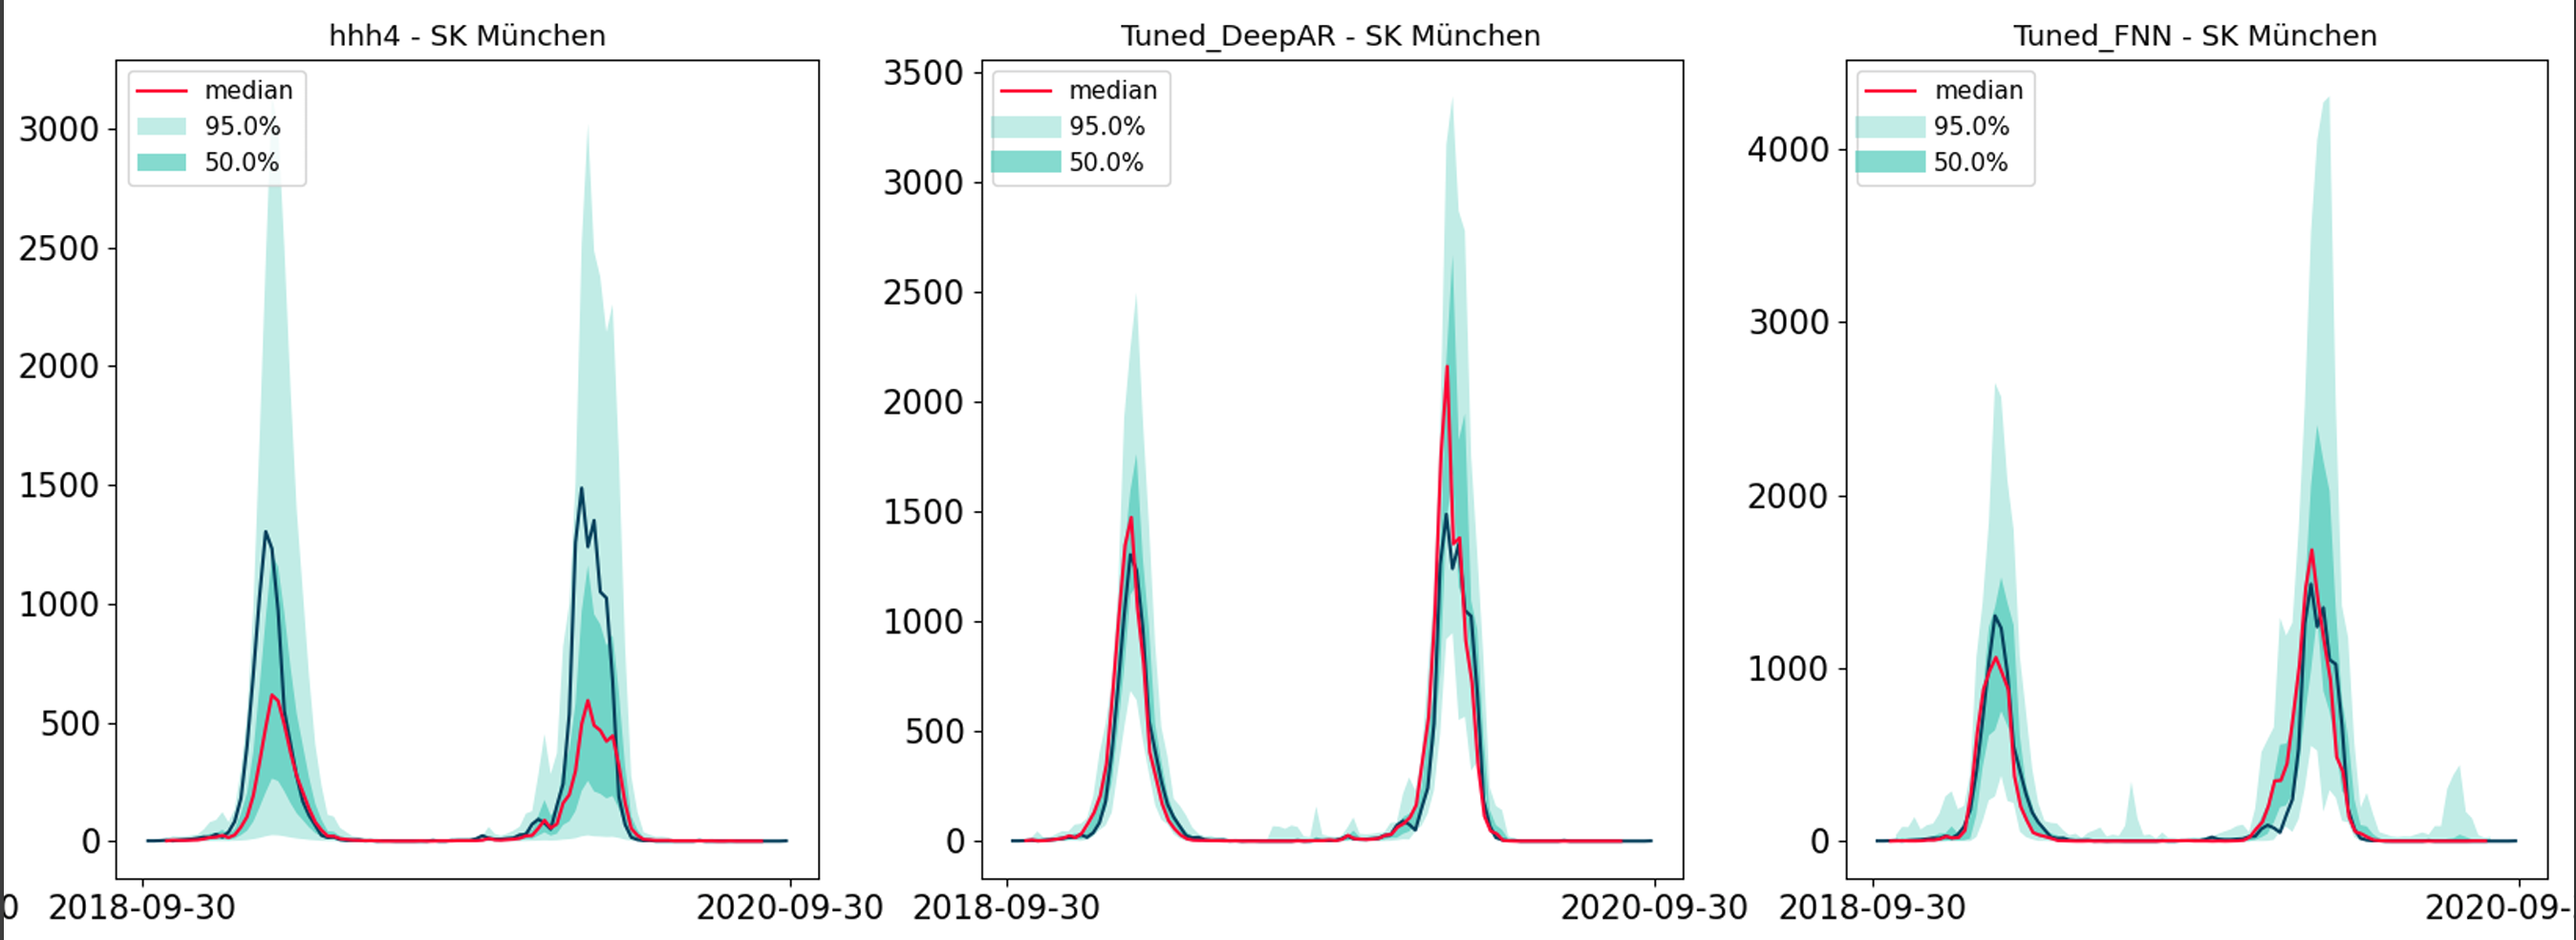
\includegraphics[trim=220 149 220 204, clip, width=\textwidth]{img/backbones/deepar.pdf}
% % 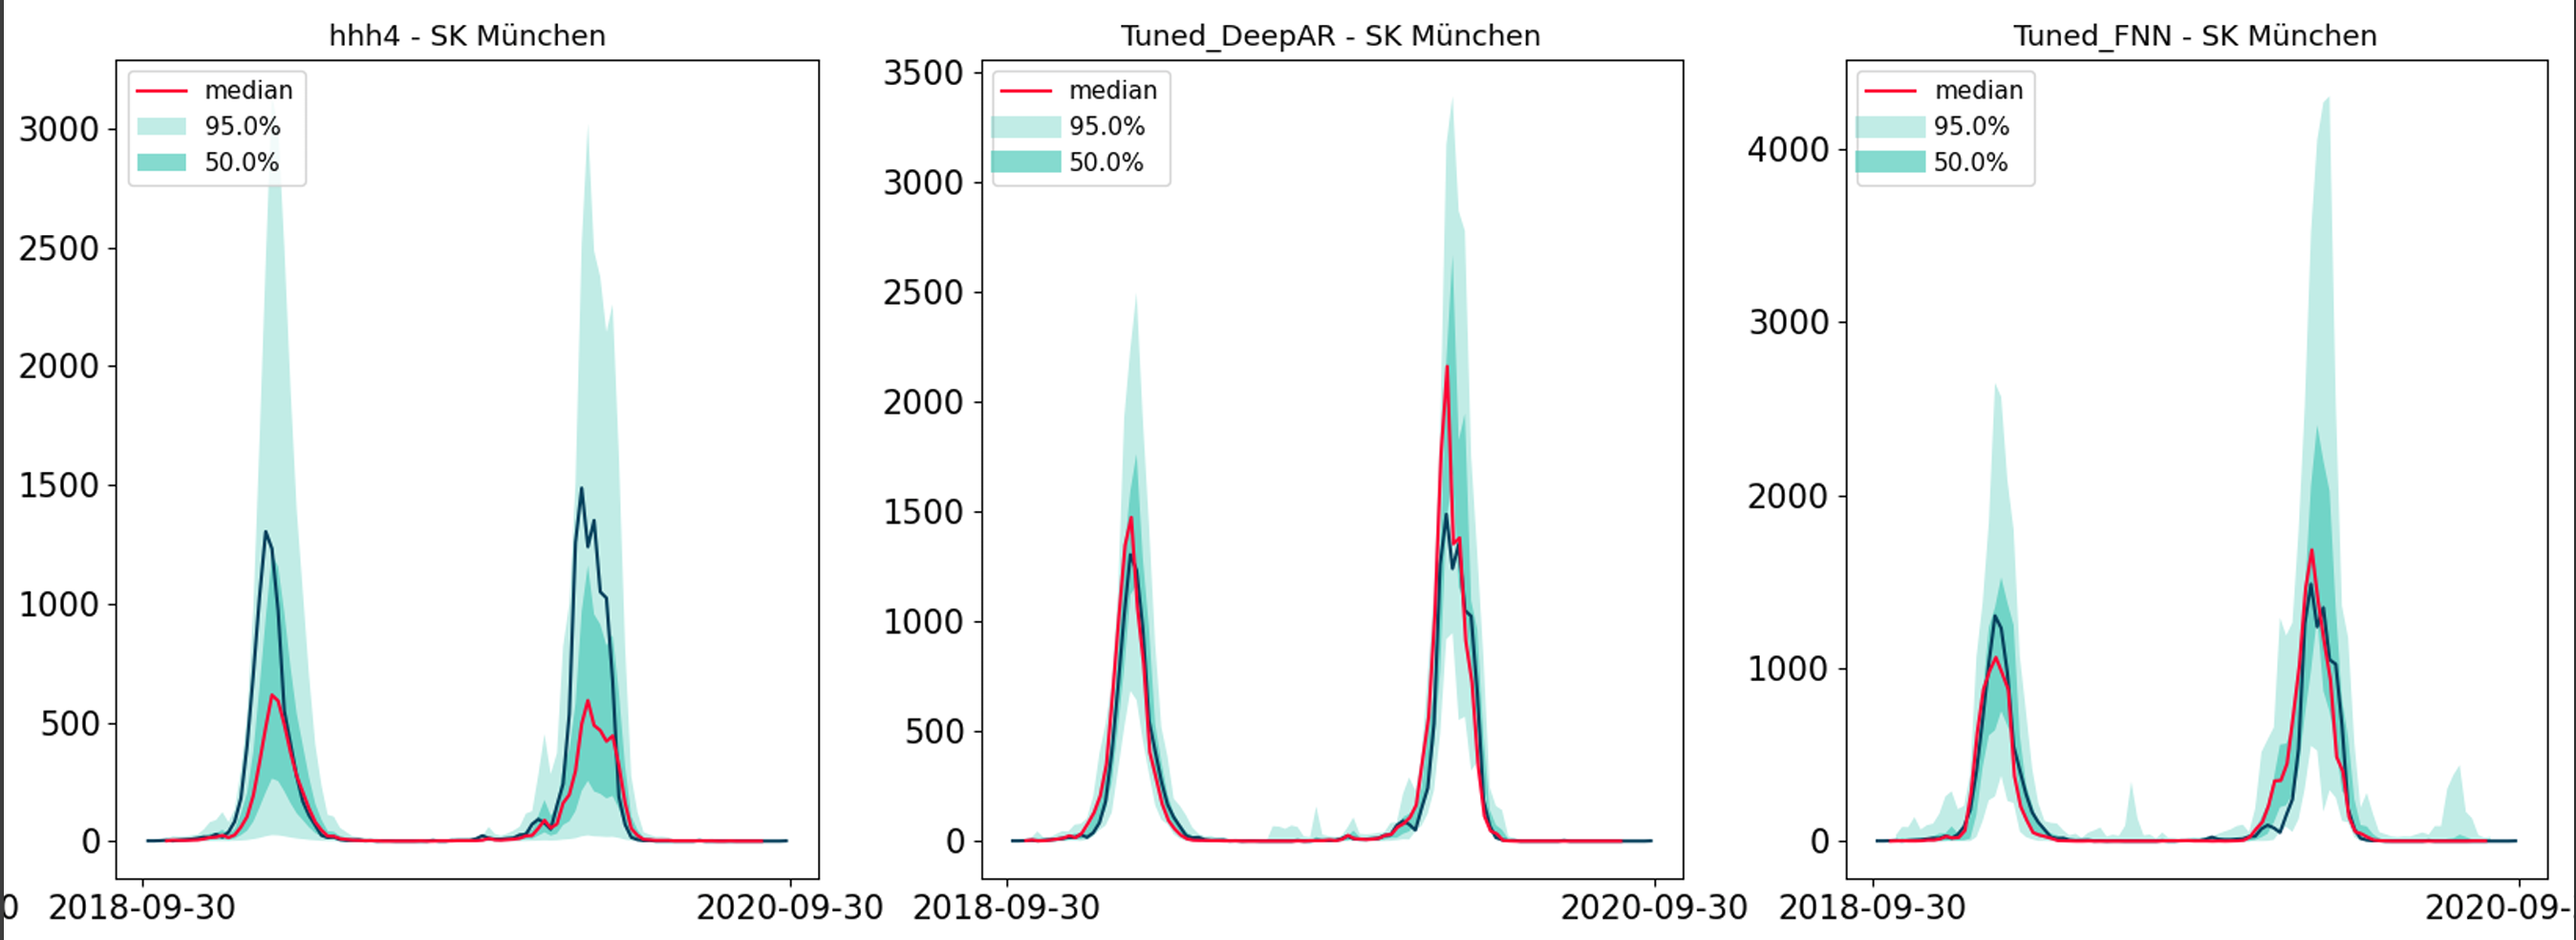
\includegraphics[trim=140 149 140 204, clip, width=\textwidth]{img/backbones/deepar.pdf}
% % \caption{Illustration of the folded DeepAR model, as implemented in BasicTS+, during training (left) and inference (right). In addition, the first step of inference is shown  unrolled in the middle.}
% % \label{fig:DeepAR}
% % \end{figure}
% % Figure \ref{fig:DeepAR} illustrates the DeepAR model \cite{salinas_deepar_2020}, a RNN-based architecture designed for channel-independent probabilistic time series forecasting.
% % % DeepAR is optimized for datasets containing large collections of related time series by learning a single global model shared across all series. 
% % The left side of Figure \ref{fig:DeepAR} shows the computations made during training and while processing the input sequence $t\in [1, L]$ during inference.
% % At each time point $t$, the model receives the previous target value ${x_{t-1}^{(i)}}$ and embeds it using a Linear layer, note that this Linear layer is an extension of BasicTS+ and is not present in the original DeepAR model of \citet{salinas_deepar_2020}.
% % In addition, known covariates ${z_{t}^{(i)}}$ are typically provided as well. This includes channel specific information that is known in advance, e.g. the time of day or the day of the week.
% % Lastly, an optional $\textit{id\_feature}^{(i)} \in \mathbb{R}^{D_{id\_feat}}$ can be included, which represents a learnable embedding of size $D_{id\_feat}$ that is independent for each channel $i$.
% % After that, the inputs are concatenated and fed to the RNN cell, in BasicTS+ the RNN cell is always set to the LSTM cell \cite{hochreiter_long_1997}.
% % In the end, the learned hidden state ${h_{t}^{(i)}}$, comprising both hidden states of the LSTM cell into one representation, is mapped to the parameters of a parametric distribution $\theta(h_{i,t})$. 
% % This distributional forecasting approach will be explained in more detail in section \ref{sec:prob_heads} about probabilistic modelling approaches.
% % Importantly, the training proceeds by maximizing the log-likelihood of observed data via teacher forcing, i.e. .
% % During inference the model is unrolled across the input values $t\in [1, L]$ equivalently to how it was discussed previously. 
% % In the first step of inference, shown in the middle of Figure \ref{fig:DeepAR}, the last input value $x_{L}^{(i)}$ and potential additional information is processed into the hidden state ${h_{L+1}^{(i)}}$.
% % Next, we again determine the predictive distribution and perform ancestral sampling where sampled outputs ˜zi, t are recursively fed back as inputs
% % for future time steps.
% % \cite{salinas_deepar_2020}, i.e. sample a value $\hat{x}_{L+1}^{(i)}$ that will be used to generate the next predictions.

% % - not implemented in BascTS+ is the time series dependent scale factor to circumvent varying magnitudes across channels/series.

% \paragraph{DeepAR.}
% \begin{figure}
% \centering
% 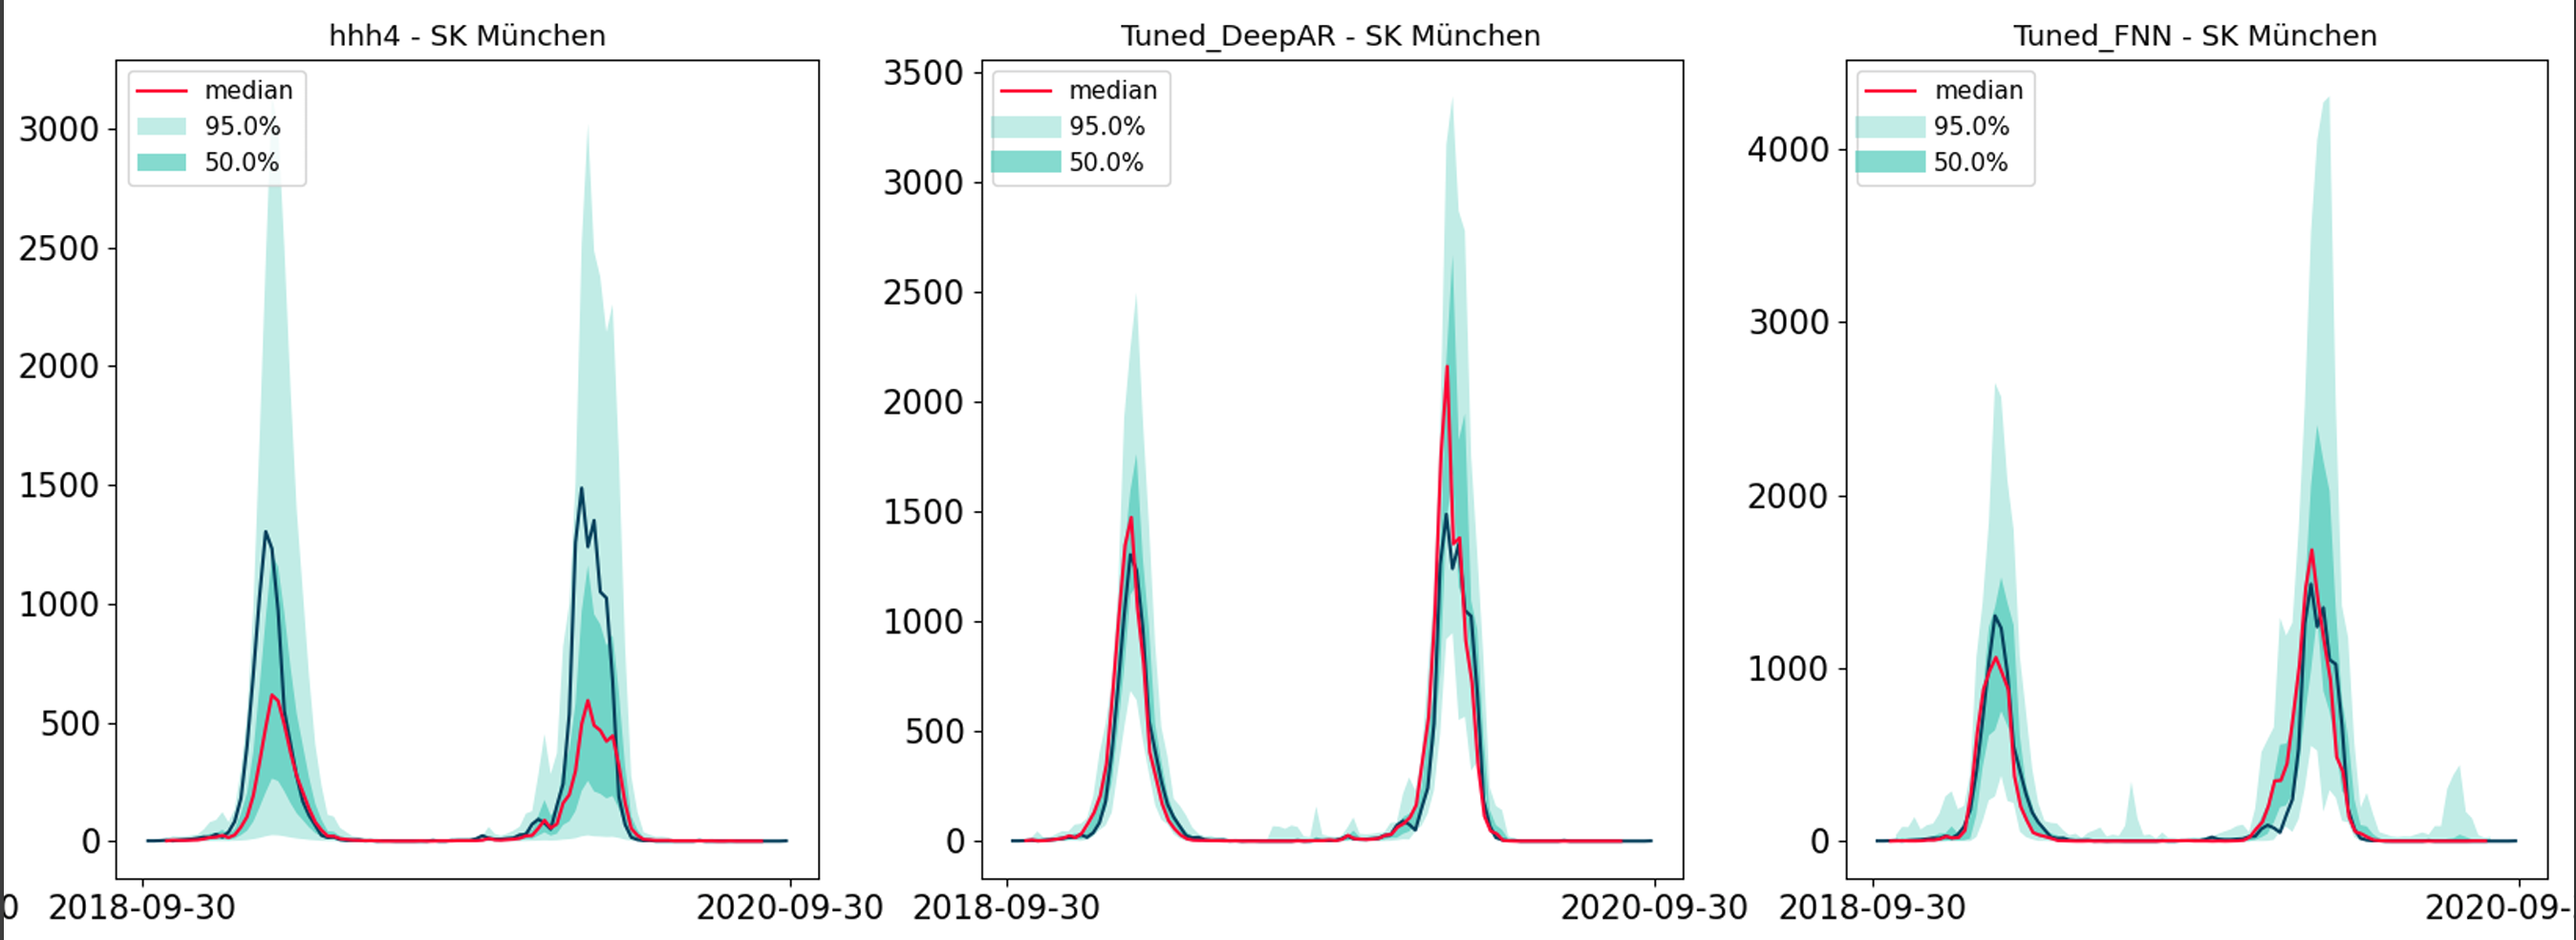
\includegraphics[trim=140 149 140 204, clip, width=\textwidth]{img/backbones/deepar.pdf}
% \caption{Schematic of the DeepAR model as implemented in BasicTS+, showing training (left), the transition to inference (middle), and recursive forecasting during inference (right). During training, the model uses teacher forcing with observed values, while inference relies on ancestral sampling.}
% \label{fig:DeepAR}
% \end{figure}
% Figure \ref{fig:DeepAR} presents the DeepAR model \cite{salinas_deepar_2020}, a RNN-based architecture designed for probabilistic, channel-independent time series forecasting. The left side of the figure illustrates the behavior during training, which is also how it processes the input sequence during inference, i.e. time steps $t \in [1, L]$.
% At each time step $t$, the model is provided with the previous target value ${x_{t-1}^{(i)}}$, allowing it to condition its predictions on the observed sequence history. This approach, known as teacher forcing \cite{williams_learning_1989}, encourages the model to stay aligned with the ground-truth trajectory during training.
% % At each time step $t$, the model receives the previous target value ${x_{t-1}^{(i)}}$ to condition its predictions to stay close to the ground-truth sequence, i.e. training with teacher forcing \cite{williiam}.
% % due to
% % the use of the ground-truth samples yt being fed back into the model to be conditioned on for the
% % prediction of later outputs. These fed back samples force the RNN to stay close to the ground-truth
% % sequence
% The previous target value ${x_{t-1}^{(i)}}$ is then embedded through a Linear layer, which is an extension introduced in BasicTS+ that was not present in the original DeepAR model.
% % Moreover, this Linear layer is an extension introduced in BasicTS+ and was not present in the original DeepAR model. 
% Additionally, known covariates ${z_{t}^{(i)}}$, e.g. time-of-day or day-of-week indicators, can be provided as well. 
% Lastly, a learnable embedding $\textit{id\_feature}^{(i)} \in \mathbb{R}^{D_{id\_feat}}$ can be included to represent channel-specific features, independent of time.
% These inputs are concatenated and passed into an RNN cell. In BasicTS+, this cell is always implemented as an LSTM cell \cite{hochreiter_long_1997}. 
% The resulting hidden state ${h_{t}^{(i)}}$, consisting of both internal LSTM states, is then mapped to the parameters of a parametric distribution $\theta(h_{t}^{(i)})$. 
% Overall, training is performed by maximizing the log-likelihood of the observed data. 
% Moreover, the implementation details of this distributional forecasting approach 
% % is only discussed briefly at this point, since it 
% will be discussed further in Section \ref{sec:prob_heads}.
% % This enables probabilistic forecasting, which will be discussed further in Section \ref{sec:prob_heads}.
% During inference, the model is unrolled over $t \in [1, L]$ in the same way as during training. 
% As shown in the middle part of Figure \ref{fig:DeepAR}, the last observed value $x_{L}^{(i)}$ and other relevant inputs are used to generate the hidden state ${h_{L+1}^{(i)}}$, from which the predictive distribution is created. 
% Since the true values $x_{L+1:L+H}^{(i)}$ are not available during inference, ancestral sampling is used instead to recursively feed back sampled values, e.g. $\hat{x}_{L+1}^{(i)}$ in Figure \ref{fig:DeepAR}. %, to predict the next step.
% % From this, the model computes a predictive distribution, from which a sample $\hat{x}_{L+1}^{(i)}$ is drawn. This sampled value is then recursively fed back into the model to predict subsequent steps via ancestral sampling \cite{salinas_deepar_2020}.
% Note, BasicTS+ does not implement the time-series-dependent scale factor originally used in DeepAR to handle varying magnitudes across different series or channels.

% % \paragraph{iTransformer}


% \section{Probabilistic TSF}
% \label{sec:prob_heads}

% % \begin{figure}
% %     \centering
% %     \includegraphics[trim=0 100 0 170, clip, width=\textwidth]{img/Prob_heads.pdf}
% %     \caption{Enter Caption}
% %     \label{fig:enter-label}
% % \end{figure}
% \begin{figure}
%     \centering
%     \includegraphics[trim=0 100 0 170, clip, width=\textwidth]{img/prob_heads/prob_heads.pdf}
%     \caption{Overview of the implemented probabilistic prediction heads. From left to right: (1) Univariate Gaussian head with separate linear layers for mean and standard deviation, using softplus to ensure positivity; (2) Quantile head that predicts a fixed set of quantiles for each time step; (3) Low-rank multivariate Gaussian head that models temporal dependencies using a low-rank plus diagonal decomposition of the covariance matrix. Each head can be used with DMS or IMS models, and adapted across different forecasting backbones.}
%     \label{fig:prob_heads}
% \end{figure}



% % Intro, whcih heads and why
% In this section, we describe how the previously introduced LTSF backbone models can be extended into probabilistic forecasting models by modifying their prediction heads and certain scaling operations. 
% % Our approach emphasizes simplicity in head design to reduce computational complexity and make the behavior of the underlying model more interpretable. 
% Specifically, to reduce computational complexity, we limit the discussion to two simpler types of probabilistic heads: parametric distributional forecasting heads, trained using the negative log-likelihood loss defined in Equation~\ref{eq:NLL}, and quantile-based forecasting heads, trained with the quantile score defined in Equation \ref{eq:QS}. 
% All four heads are displayed in Figure \ref{fig:prob_heads}.
% We assume that the backbone model produces embeddings $h \in \mathbb{R}^{N \times D}$, which are then passed to the probabilistic head.
% % write that for DLinear it is a bit different since the head is applied to the end -> describe how the head is applied
% In the case of DLinear, the probabilistic head is either added after the seasonal and trend components or used to replace each of the two linear layers directly. For PatchTST and DeepAR, the probabilistic heads substitute the original prediction heads. Notably, in DeepAR, when using quantile heads, the iterative sampling process takes the median forecast instead of sample forecasts at each step.
% Furthermore, Figure~\ref{fig:prob_heads} illustrates the setup for DMS methods, where the prediction head generates the entire forecast horizon $H$ in a single forward pass. The same head architectures can also be used in IMS models by configuring them to output only one step at a time, achieved by setting $H=1$ during head initialization.
% % - choose simpler heads to lighten the computational load, while also emphisizing the behavior of the underlying model
% % - train parametric distributional forecasting methods via NLL in Equation~\ref{eq:NLL}
% % - train quantile methods via QL
% % - we assume that the backbone model forwards the embeddings $h \in \mathbb{R}^{N \times D}$ to the probabilistic head with embedding dimension $D$, in which DMS methods produce the forecasts in one go by setting the returning length to $H$. In contrast, not shown IMS models forecast only the next step in the corresponding heads. 
% % we chose simple parametric distributional forecasting. 
% % Since some other methods encounter the densitiy spike issue if trained or tuned for NLL \cite{bergsma_c2far_2022}

% % univariate prediction head
% \paragraph{Univariate head.}
% The left side of Figure~\ref{fig:prob_heads} illustrates the univariate probabilistic prediction head, shown here using a Gaussian head as an example. This architecture consists of two separate linear layers: one predicts the mean, and the other predicts the standard deviation. To guarantee that the standard deviation remains strictly positive, the output of its corresponding layer is passed through a softplus activation function, as done in \cite{salinas_deepar_2020, salinas_high-dimensional_2019, sprangers_parameter-efficient_2023}, which is defined as
% \begin{equation}
%  \text{softplus}(x) = \log(1 + e^{x})
%     \label{eq:softplus}
% \end{equation}
%  % is applied to its output, as done in \cite{salinas_deepar_2020, salinas_high-dimensional_2019, sprangers_parameter-efficient_2023}.
% % Under the Deep Markov State (DMS) formulation, it assumes independence across dimensions. 
% Finally, the predicted parameters are concatenated to form $\hat{\theta}_{L+1:L+H} \in \mathbb{R}^{N \times H \times 2}$. %, where each entry contains the mean and standard deviation and thus the distribution for a predicted time step. 
% Alternative univariate distributional heads follow the same structure but modify the output layers to parameterize different distributions. For instance, the Laplace head mirrors the Gaussian setup but substitutes the likelihood function. The Student’s t-distribution head extends the architecture by introducing a third linear layer to estimate the degrees of freedom for each time step. This output is also passed through a softplus activation and shifted by a scalar of 1 to ensure the minimum degree of freedom is at least one.
% % - Laplace equivalent to gaussian, just different distribution is used
% % - student t also models the degrees of freedom of each times step via a third linear layer, that also employs a softplus and adds elemtnwise scalar of 1 such that the lowest degreee is ensured to be 1.  
% % On the left of Figure \ref{fig:prob_heads}, the univariate prediction head is shown. 
% % - consists of two linear layers, one for each parameter, e.g. mean and std of gaussian.
% % - in the DMS formulation assumes independence
% % - ensure positive oriented standard deviation via softplus function
% % - lastly concat the parameters to produce $\hat{\theta}_{L+1:L+H}\in \mathbb{R}^{N\times H \times 2}$
% % - models with this prediction head are trained using NLL, see Equation \ref{eq:NLL}.
% % multivariate 
% \paragraph{Multivariate head.}
% To the right of the univariate head in Figure~\ref{fig:prob_heads}, the multivariate Gaussian prediction head is shown. 
% The mean is computed analogously to the univariate case via a linear projection. For the covariance, we adopt a low-rank plus diagonal decomposition~\cite{wu_high-dimensional_2020}, which drastically reduces computational complexity (especially when the rank \( R \ll H \)) and introduces a natural regularization effect, as the low-rank structure captures dominant modes of variability while the diagonal component accounts for residual uncertainty (similar to probabilistic PCA \cite{tipping_probabilistic_1999}).
% Formally, the covariance decomposition is defined as:
% \begin{equation}
% \hat{\Sigma}^{(i)} = (\hat{L}^{(i)} {\hat{L}^{(i)}})^\top + \hat{D}^{(i)}
% \label{eq:multivariate_cov}
% \end{equation}
% Here, for each time series $i=1,\dots,N$, the predicted distribution is modeled as a multivariate Gaussian with mean $\hat{\mu}^{(i)} \in \mathbb{R}^H$ and covariance matrix $\hat{\Sigma}^{(i)}\in \mathbb{R}^{H\times H}$. 
% The low-rank component $\hat{L}^{(i)} \in \mathbb{R}^{H\times R}$ captures shared structure, while $\hat{D}^{(i)} \in \mathbb{R}^{H}$ represents the diagonal noise. 
% The diagonal matrix is constructed by placing the softplus-activated entries of $\hat{D}^{(i)}$ along the diagonal. 
% % Altogether, this ensures positive semi-definiteness since (\cite{wu_high-dimensional_2020, horn_chapter_2012}).
% % Altogether, this ensures positive semi-definiteness since both terms are positive semi-definite by construction: the product $(\hat{L}^{(i)} {\hat{L}^{(i)}})^\top$ forms a Gram matrix, which is always positive semi-definite \cite{horn_chapter_2012}, %Observation 7.2.10
% % and the diagonal matrix formed by softplus-activated entries is strictly positive on the diagonal, thus also positive definite \cite{horn_chapter_2012}.
% % Furthermore, the sum of a positive-definite and a positive-semidefinite matrix is also positive-definite \cite{horn_chapter_2012}. % Observation 7.1.3
% Altogether, this construction guarantees positive definiteness of the resulting covariance matrix. Concretely, the term $(\hat{L}^{(i)} {\hat{L}^{(i)}})^\top$ is a Gram matrix and therefore positive semi-definite by definition~\cite[Observation 7.2.10]{horn_chapter_2012}. The diagonal component, obtained by applying the softplus function to $\hat{D}^{(i)}$, yields strictly positive entries and thus forms a positive-definite diagonal matrix by design~\cite{horn_chapter_2012}. Since the sum of a positive-definite and a positive semi-definite matrix is itself positive-definite~\cite[Observation 7.1.3]{horn_chapter_2012}, the resulting covariance matrix $\hat{\Sigma}^{(i)}$ is guaranteed to be positive-definite.
% % -However there are also cases where numercial instabilities hinder this and training is stopped
% %By the closure of the positive semi-definite cone under addition~\cite{horn_chapter_2012}, the resulting covariance matrix Σ^(i)Σ^(i) is guaranteed to be positive semi-definite~\cite{wu_high-dimensional_2020}.
% %
% The parameters $\hat{\theta}_{L+1:L+H} \in \mathbb{R}^{N \times H \times R+2}$, containing the predicted mean, low-rank factors, and diagonal entries, are passed to the \texttt{LowRankMultivariateNormal} class from \texttt{torch.distributions}\footnote{\href{https://docs.pytorch.org/docs/stable/distributions.html}{https://docs.pytorch.org/docs/stable/distributions.html}} to receive the multivariate density. 
% In contrast to the univariate prediction head, \texttt{torch.distributions} does not support alternative low-rank multivariate distribution types, hence limiting us to the low-rank multivariate Gaussian distribution.
% % restricts the multivariate output to the low-rank Gaussian form, as it does not support alternative multivariate distribution types.

% % Quantile
% % Third from the left in Figure \ref{fig:prob_heads} is the depiction of the Quantile head.
% % - for this we pre-determine $Q$ quantile levels
% % - for each quantile level, we map the backbone embeddings $h\in \mathbb{R}^{N\times D}$ to a quantile forecast resulting in $\hat{x}_{L+1:L+H} \in \mathbb{R}^{N\times H \times Q}$
% \paragraph{Quantile head.} 
% Third from the left in Figure~\ref{fig:prob_heads} is the depiction of the Quantile head. In this approach, we pre-determine a fixed set of \( Q \) quantile levels. For each of these quantile levels, the backbone embeddings \( h \in \mathbb{R}^{N \times D} \) are mapped independently to produce corresponding quantile forecasts. This results in an output tensor \( \hat{x}_{L+1:L+H} \in \mathbb{R}^{N \times H \times Q} \), where each slice along the third dimension represents the forecast for a specific quantile level.
% For the quantile DeepAR model, we feed back the previously predicted median value during inference.
% % Although this prediction head is comparably simple, 
% % Notably, the quantile crossing problem plus retraining for new quantile levels

% \paragraph{Implicit Quantile Network head.}
% Lastly, the IQN prediction head, shown on the right side of Figure~\ref{fig:prob_heads}, is adapted from the architecture proposed by \citet{gouttes_probabilistic_2021} and \citet{dabney_implicit_2018}. The prediction process begins by sampling a quantile level \( u \) from the \texttt{Uniform(0, 1)} distribution. This quantile level is then embedded into a representation \( \phi_u \) using positional encoding as defined by:
% \begin{equation}
%     \phi_u = \mathrm{ReLU}\!\Bigl(\mathrm{Linear}\big(\cos(u \cdot i \cdot \pi)\big)\Bigr)
%     \label{eq:phi_u}
% \end{equation}
% where \( i \in \mathbb{R}^{C_E} \) is a fixed vector of values linearly spaced from 1 to \( C_E \),  \( C_E \) is a hyperparameter controlling the dimension of the cosine embedding. The linear layer in Equation~\ref{eq:phi_u} projects from the cosine embedding dimension \( C_E \) to a quantile embedding dimension \( Q_E \), another tunable hyperparameter. 
% To match the number of time series instances, \( \phi_u \in \mathbb{R}^{
% Q_E} \) is broadcast into  \( \phi_u \in \mathbb{R}^{N \times Q_E} \) by repeating the same embedding \( N \) times. This quantile embedding is then concatenated with the backbone representation \( h \in \mathbb{R}^{N \times D} \), resulting in a combined representation of shape \( \mathbb{R}^{N \times (D + Q_E)} \). A final linear projection maps this to the forecast output \( \hat{x}_{L+1:L+H} \in \mathbb{R}^{N \times H} \).
% In addition to the concatenation approach, we optionally support the original formulation from \citet{gouttes_probabilistic_2021}, which replaces concatenation with a Hadamard product:
% \begin{equation}
%     \hat{x}_{L+1:L+H} = \mathrm{Linear}\big( h \odot (1+\phi_u)\big)
% \end{equation}
% Notably, this formulation requires that \( Q_E = D \), which varies across model and hyperparameter choices. 
% During training, the quantile level \( u \) is resampled for each training batch, and the sampled value is stored to compute the quantile loss. 
% Since we are interested in forecasts that represent a consistent quantile level across all prediction steps, we sample a random quantile level per forecast horizon rather than resampling one every time step.
% However, the IQN DeepAR model is an exception to this, since we follow the IMS approach in \citet{gouttes_probabilistic_2021}, by sampling a new quantile level for every time step.
% The reason for this is that a constant quantile level led to divergent predictions, as shown in the Appendix \ref{ch:additional_exp} in Figure \ref{fig:iqn_deepar_diverges}.
% % This aligns closer with our inference setting, where we are interested in forecasts that are conditioned on a consistent quantile level across all prediction steps.
% % Furthermore, regarding the IQN DeepAR model, we follow the IMS approach in \citet{gouttes_probabilistic_2021}, by sampling a new quantile level for every time step, since a constant
% % a single quantile level per forecast horizon rather than resampling one every time step. 
% % produce forecasts conditioned on a consistent quantile level across all prediction steps.
% % - use the same quantiles to evaluate the model though i.e. during validation/testing, also infleunces the hypereparmeter search

% % IQN
% % - the IQN prediction head is depicted on the right side of Figure \ref{fig:prob_heads}
% % - we adpated the IQN architecture from \citet{gouttes_probabilistic_2021, dabney_implicit_2018}
% % - here the first step taken is to sample a quantile level $u$ from the \texttt{Uniform(0, 1)} distribution
% % - this quantile level is then embedded into $\phi_u$ using positional encoding with 
% % \begin{equation}
% %     \phi_u = \mathrm{ReLU}\!\Bigl(\mathrm{Linear}\big(\cos(u \cdot i \cdot \pi)\big)\Bigr)
% %     \label{eq:phi_u}
% % \end{equation}
% % with $i \in \mathbb{R}^{C_E}$ a vector of numbers arranged from 1 to $C_E$, where $C_E$ is a hyperparameter that controls the dimension of the cosine embedding.
% % The Linear layer in Equation \ref{eq:phi_u} maps from the cosine embedding dimension $C_E$ to the quantile embedding dimension $Q_E$, whcih is yet another hyperparameter. 
% % The final quantile representation $\phi_u \in \mathbb{R}^{N\times Q_E}$ is then achieved by sharing the same embedding $\phi_u$ across series by repeating/stacking $\phi_u$ $N$ times.
% % After that, $\phi_u$ and $h\in \mathbb{R}^{N\times D}$ are concatenated along the series axis, resulting in an embedding with size $\mathbb{R}^{N\times D+ Q_E}$, which is projected into the forecast $\hat{x}_{L+1:L+H} \in \mathbb{R}^{N\times H}$ by a final Linear layer.
% % Alternatively to the concatenation shown in Figure \ref{fig:prob_heads}, we also optionally added the original implementation in \citet{gouttes_probabilistic_2021}, which uses a hadamard product $\odot$ like this:
% % \begin{equation}
% %     \hat{x}_{L+1:L+H} = \mathrm{Linear}\big( h \odot (1+\phi_u)\big)
% % \end{equation}
% % Notably, this requires setting $Q_E=D$.
% % In the end, the originally sampled quantile level is stored to compute the quantile loss for the predictions, and is resampled for every new training step.
% % - we also do not sample a quantile level across the whole horizon, different from the IMS approach used in \cite{gouttes_probabilistic_2021} since our inference setup is also interested in producing forecasts given one quantile level that is the same across all prediction steps.


% % During training, a quantile level $\tau \sim \mathcal{U}(0, 1)$ is sampled for each element in the batch, such that . 
% % This contrasts the time step wise quantile level sampling, because it simplifies loss calculation and is equivalent to how we use the module during inference, i.e. specifying a quantile level for which we want to produce the forecast. In addition, it is actually the same for autoregressive models... 


% % bergsma c2far 2.2
% % Unfortunately, fitting powerful continuous models to discrete/mixed data “can lead to arbitrarily high
% %  density values, by locating a narrow high density spike on each of the possible discrete values” [71].
% % While this is a known issue in image modeling [69], 
% % Density models based onsplines [26] or flows[54]shouldtherefore not be trained directly to maximize
% %  likelihood, as this may guide parameters (e.g., spline knot positions) solely to enable density spikes.
% %  Apotential solution is dequantizing, e.g., adding Uniform[0,1] noise as in [54].
% % \textbf{IQN}
% % We adapt the Implicit Quantile Network (IQN) architecture \cite{gouttes_probabilistic_2021, dabney2018implicit, gouttes2021probabilistic} to serve as the probabilistic prediction head in our time series model. 
% % It is depicted in Figure ...
% % During training, a quantile level $\tau \sim \mathcal{U}(0, 1)$ is sampled for each element in the batch, such that . 
% % This contrasts the time step wise quantile level sampling, because it simplifies loss calculation and is equivalent to how we use the module during inference, i.e. specifying a quantile level for which we want to produce the forecast. In addition, it is actually the same for autoregressive models... 
% % The quantile $\tau$ is embedded using a cosine basis expansion followed by a learnable linear transformation and a ReLU activation, resulting in the embedding $\phi(\tau) \in \mathbb{R}^{d}$. This embedding is combined with the input feature vector $x \in \mathbb{R}^{d}$ via an elementwise Hadamard product: $x \odot (1 + \phi(\tau))$. The result is passed through a linear output layer to produce the final quantile prediction for the prediction horizon. 
% % At inference time, we compute forecasts in the same way, however the process is repeated for each quantile provided of a pre-determined quantile level set, which we set to the same quantile levels for which we train the normal quantile regression heads as well, resulting in an equal ground for evaluation.
% % fixed set of quantile levels by repeating this process for each $\tau \in \{\tau_1, \dots, \tau_K\}$. 
% % Our adaptation supports both autoregressive and non-autoregressive forecasting setups, and can be extended to multivariate settings.
% % - show the figure here

% % SCALING
% \paragraph{Scaling transformations for distributional parameters.}
% \label{sec:scaling}
% % - The BasicTS benchmark provides two commonly used scaling operations. Z-score normalization and Min-Max normalization.


% % Scaling operations are applied prior to the model call, whereas de-scaling operations are called after the model's output has been obtained.
% % In BasicTS+, the two provided scaling operations are Z-score normalization and Min-Max normalization.
% % On top of that, some methods, e.g. PatchTST, have the option to additionally perform revIn scaling (potentially involves trainable operations, therefore not a standard scaler that is applied to every model)
% % First,  scaling is performed on the input batch $x_{1:L} \in \mathbb{R}^{B \times L \times N}$ with $B$ batch elements, input length $L$ and $N$ series.
% % For Z-score normalization this can be expressed as:
% % \begin{equation}
% %     \tilde{x}_{1:L} = \frac{x_{1:L} - \mu}{\sigma},
% %     \label{eq:zscore_norm}
% % \end{equation}
% % Here, $\mu \in \mathbb{R}^{B\times N}$ and $\sigma \in \mathbb{R}^{B\times N}$ are the sample mean and variance computed based on each individual batch element and channel. 
% % For Min-Max Scaling this can be 
% Scaling operations play a central role in time series modeling pipelines, due to varying scales across series, e.g. power law distribution in retail sales series \cite{salinas_deepar_2020, salinas_high-dimensional_2019}, and distribution shifts across time \cite{fan_dish-ts_2023, zhang_probts_2024, kim_reversible_2021, nie_time_2022}. %[CITATION- and particularly in time series operations due to the distribution shift problem]. 
% In the BasicTS+ benchmark two commonly used scaling operations, Z-score normalization and Min-Max normalization, are provided. 
% These transformations are implemented such that they surround the model, i.e. scaling is applied before the model is called and inverse transformations (de-scaling) are performed after model outputs are obtained to restore predictions to their original scale.
% % Note, that we would have had the option if we wanted to rescale, however we always perfrom rescaling such that models results are comparable, including NLL and QL values of the same model in HPO.
% We always apply inverse-scaling to ensure model outputs and resulting losses as well as scores are directly comparable.
% The scaling operation is first applied to the input batch \( x_{1:L} \in \mathbb{R}^{B \times L \times N} \), with batch size $B$, input sequence length $L$, and \( N \) number of series. 
% % Z STANDARDIZATION 
% For Z-score normalization, the transformation is defined as:
% \begin{equation}
% \tilde{x}_{1:L} = \frac{x_{1:L} - \tilde{\mu}}{\tilde{\sigma}},
% \end{equation}
% where \( \tilde{\mu} \in \mathbb{R}^{N} \) and \( \tilde{\sigma} \in \mathbb{R}^{N} \) are the mean and standard deviation per series computed over the entire train set. %each batch element and channel. 
% Note that BasicTS+ also allows using a single scalar mean and standard deviation shared across all series, i.e. \( \tilde{\mu} \in \mathbb{R} \) and \( \tilde{\sigma} \in \mathbb{R} \). 
% However, the upcoming re-scaling computations remain formally identical, as these scalars can be interpreted as constant vectors of dimension $N$, yielding the same expressions.
% % MIN MAX
% For Min-Max normalization, the transformation is:
% \begin{equation}
% \tilde{x}_{1:L} = \frac{x_{1:L} - \tilde{x}_{\min}}{\tilde{x}_{\max} - \tilde{x}_{\min}},
% \end{equation}
% where \( \tilde{x}_{\min}, \tilde{x}_{\max} \in \mathbb{R}^{N} \) are the minimum and maximum values per series over the train set, ultimately scaling values into the \([0,1]\) range.
% % resulting in train set values scaled to \([0,1]\). %, and \( a, b \) denote the target range (e.g., \([0,1]\)).
% % In addition to this, the RevIN \cite{kim_reversible_2021} operation is available for the PatchTST model as well.
% % However, as described in Equation \ref{eq:revin}, the operation is not performed across the whole train set. Instead, the parameters $\mu^{(i)}, \space \sigma^{(i)}, \space \gamma, \space \beta \in \mathbb{R}^N$ are determined or learned per series and per batch.
% In addition to this, the RevIN operation \cite{kim_reversible_2021} is available for the PatchTST model. Unlike the other two scaling methods, RevIN computes the parameters $\tilde{\mu}^{(i)}, \space \tilde{\sigma}^{(i)}, \space \gamma, \space \beta \in \mathbb{R}^N$ per series and per batch, as shown in Equation~\ref{eq:revin}.
% After the model produces outputs in the scaled space, these outputs must be mapped back. 
% While the re-scaling operation for point and quantile forecasts is straightforward, parametric distributional forecasting methods have to be handled differently.
% For univariate distributions with location and scale parameters, such as Gaussian outputs with predicted mean \( \hat{\mu} \in \mathbb{R}^{B \times H \times N}\) and standard deviation \( \hat{\sigma} \in \mathbb{R}^{B \times H \times N}\), this descaling is:
% \begin{itemize}
%     \item \textbf{Z-score de-normalization:}
%     \begin{equation}
%     \mu = \hat{\mu} \cdot \tilde{\sigma} + \tilde{\mu}, \quad \sigma = \hat{\sigma} \cdot \tilde{\sigma}
%     \end{equation}
%     \item \textbf{Min-Max de-normalization:}
%     \begin{equation}
%     \mu = \hat{\mu}\cdot R + \tilde{x}_{\min}, \quad \sigma = \hat{\sigma} \cdot R, \quad \text{where } R = \tilde{x}_{\max} - \tilde{x}_{\min}
%     \end{equation}
%      \item \textbf{RevIN de-normalization:} (following normalization as in Equation \ref{eq:revin}) 
%     \begin{equation}
%     \mu^{(i)} = \left( \frac{\hat{\mu}^{(i)} - \beta^{(i)}}{\gamma^{(i)}} \right) \cdot \tilde{\sigma}^{(i)} + \tilde{\mu}^{(i)}, \quad 
%     \sigma^{(i)} = \hat{\sigma}^{(i)} \cdot \frac{\tilde{\sigma}^{(i)}}{\gamma^{(i)}}
%     \end{equation}
% \end{itemize}
% % \textbf{Z-score de-normalization:}
% % \begin{equation}
% % \mu = \hat{\mu} \cdot \tilde{\sigma} + \tilde{\mu}, \quad \sigma = \hat{\sigma} \cdot \tilde{\sigma}
% % \end{equation}
% % \\
% % \textbf{Min-Max de-normalization:}
% % \begin{equation}
% % \mu = \hat{\mu}\cdot R + \tilde{x}_{\min}, \quad \sigma = \hat{\sigma} \cdot R, \quad \text{where } R = \tilde{x}_{\max} - \tilde{x}_{\min}
% % \end{equation}
% In the multivariate setting, we assume the model produces forecasts for each of the \( N \) series independently over a forecast horizon of length \( H \). Concretely, for each series \( i = 1, \dots, N \), the predicted distribution is a multivariate Gaussian with parameters \( \hat{\mu}^{(i)} \in \mathbb{R}^H \) and covariance \( \hat{\Sigma}^{(i)} = ( \hat{L}^{(i)} \hat{L}^{(i)})^\top + \hat{D}^{(i)} \), where \( \hat{L}^{(i)} \in \mathbb{R}^{H \times r} \) and \( \hat{D}^{(i)} \in \mathbb{R}^{H \times H} \) is diagonal.
% The de-normalization is applied per series, using the original scaling parameters \( \tilde{\mu}^{(i)} \), \( \tilde{\sigma}^{(i)} \), or \( \tilde{x}_{\min}^{(i)} \), \( \tilde{x}_{\max}^{(i)} \) of each series.
% \\
% \begin{itemize}
%     \item \textbf{Z-score de-normalization:}
%     \begin{align}
%     \label{eq:de_mu}
%     \mu^{(i)} &= \hat{\mu}^{(i)} \cdot \tilde{\sigma}^{(i)} + \tilde{\mu}^{(i)}, \\
%     \label{eq:de_sig}
%     \Sigma^{(i)} &= (\tilde{\sigma}^{(i)})^2 \cdot \hat{\Sigma}^{(i)} = (\tilde{\sigma}^{(i)})^2 \cdot \big((\hat{L}^{(i)} \hat{L}^{(i)})^\top + \hat{D}^{(i)}\big)
%     \end{align}
%     \item \textbf{Min-Max de-normalization:} Let \( R^{(i)} = \tilde{x}_{\max}^{(i)} - \tilde{x}_{\min}^{(i)} \), then simply substitute $\tilde{\mu}^{(i)}$ and $(\tilde{\sigma}^{(i)})^2$ in Equation \ref{eq:de_mu} and \ref{eq:de_sig} by $\tilde{x}_{\min}^{(i)}$ and $(R^{(i)})^2$ respectively.
%     % \begin{align}
%     % % \mu^{(i)} &= \hat{\mu}^{(i)} \cdot R^{(i)} + \tilde{x}_{\min, i}, \\
%     % % \Sigma^{(i)} &= (R^{(i)})^2 \cdot \hat{\Sigma}^{(i)} = (R^{(i)})^2 \cdot \big((\hat{L}^{(i)} \hat{L}^{(i)})^\top + \hat{D}^{(i)}\big)
%     % \end{align}
%     \item \textbf{RevIN de-normalization:} (following normalization as in Equation \ref{eq:revin}) 
%     \begin{align}
%     % \mu^{(i)} &= (\gamma^{(i)} \cdot \hat{\mu}^{(i)} - \beta^{(i)}) \cdot \tilde{\sigma}^{(i)} + \tilde{\mu}^{(i)}, \\
%     % \sigma^{(i)} &= \gamma^{(i)} \cdot \hat{\sigma}^{(i)} \cdot \tilde{\sigma}^{(i)}\\
%     \mu^{(i)} &= \left( \frac{\hat{\mu}^{(i)} - \beta^{(i)}}{\gamma^{(i)}} \right) \cdot \tilde{\sigma}^{(i)} + \tilde{\mu}^{(i)}, \\
%     \Sigma^{(i)} &= \left( \frac{\tilde{\sigma}^{(i)}}{\gamma^{(i)}} \right)^2 \cdot \hat{\Sigma}^{(i)} = \left( \frac{\tilde{\sigma}^{(i)}}{\gamma^{(i)}} \right)^2 \cdot \left( \hat{L}^{(i)} (\hat{L}^{(i)})^\top + \hat{D}^{(i)} \right)
%     \end{align}
% \end{itemize}


% % \textbf{Z-score de-normalization:}
% % \begin{align}
% % \mu^{(i)} &= \hat{\mu}^{(i)} \cdot \tilde{\sigma}^{(i)} + \tilde{\mu}^{(i)}, \\
% % \Sigma^{(i)} &= (\tilde{\sigma}^{(i)})^2 \cdot \hat{\Sigma}^{(i)} = (\tilde{\sigma}^{(i)})^2 \cdot \big((\hat{L}^{(i)} \hat{L}^{(i)})^\top + \hat{D}^{(i)}\big)
% % \end{align}
% % \\
% % \textbf{Min-Max de-normalization:} Let \( R^{(i)} = \tilde{x}_{\max, i} - \tilde{x}_{\min, i} \), then:
% % \begin{align}
% % \mu^{(i)} &= \hat{\mu}^{(i)} \cdot R^{(i)} + \tilde{x}_{\min, i}, \\
% % \Sigma^{(i)} &= (R^{(i)})^2 \cdot \hat{\Sigma}^{(i)} = (R^{(i)})^2 \cdot \big((\hat{L}^{(i)} \hat{L}^{(i)})^\top + \hat{D}^{(i)}\big)
% % \end{align}


% % For multivariate distributions, e.g., multivariate Gaussians with low-rank covariance decompositions, similar inverse transformations apply. Let \( \hat{\Sigma} = \hat{L}\hat{L}^\top + \hat{D} \) in the scaled space with \( \hat{L} \in \mathbb{R}^{H \times r} \), \( \hat{D} \in \mathbb{R}^{H \times H} \) diagonal.
% % \\
% % \textbf{Z-score de-normalization:}
% % \begin{align}
% % \mu &= \hat{\mu} \cdot \tilde{\sigma} + \tilde{\mu}, \\
% % \Sigma &= (\hat{L}\tilde{S})(\hat{L}\tilde{S})^\top + S \hat{D} S,
% % \end{align}
% % where \( \tilde{S} = \text{diag}(\tilde{\sigma}_1, \dots, \tilde{\sigma}_H) \).
% % \\
% % \textbf{Min-Max de-normalization:}
% % \begin{align}
% % A &= \text{diag}\left(\frac{1}{R_i}\right), \quad c_i = - A_{ii} x_{\min,i}, \\
% % \mu &= A^{-1}(\hat{\mu} - c), \\
% % \Sigma &= (A^{-1} L)(A^{-1} L)^\top + A^{-1} D A^{-1}.
% % \end{align}
% % This transformation ensures that probabilistic outputs remain consistent and interpretable in the original data space, and that any likelihood computation reflects the original units and distributions of the input series.

% % - also need to add revin

% % Consider a random variable or vector \( X \) and its scaled version \( \tilde{X} \). We describe the transformations needed to map parameters of univariate and multivariate distributions between the scaled and original spaces.

% % \bigskip

% % \noindent
% % \textbf{1. Min-Max Scaling:}  
% % Given scaling to \([a, b]\) by
% % \[
% % \tilde{X} = a + \frac{X - \min(X)}{\max(X) - \min(X)} (b - a),
% % \]
% % define
% % \[
% % X_{\min} = \min(X), \quad X_{\max} = \max(X), \quad R = X_{\max} - X_{\min}.
% % \]

% % \bigskip

% % \noindent
% % \textbf{Univariate distributions:}  
% % If the scaled distribution has parameters \(\tilde{\mu}, \tilde{\sigma}\), the original parameters are
% % \[
% % \mu = \frac{\tilde{\mu} - a}{b - a} R + X_{\min},
% % \quad
% % \sigma = \frac{R}{b - a} \tilde{\sigma}.
% % \]

% % For example, for a Gaussian \( \mathcal{N}(\tilde{\mu}, \tilde{\sigma}^2) \), the original parameters are obtained by linear inverse transformation.

% % \bigskip

% % \noindent
% % \textbf{Multivariate Gaussian with low-rank covariance:}

% % Let
% % \[
% % \tilde{X} = A X + c,
% % \]
% % where for min-max scaling on each dimension \( i \),
% % \[
% % A = \text{diag}\left(\frac{b - a}{R_i}\right), \quad
% % c = a - \frac{b - a}{R_i} X_{\min,i}.
% % \]

% % Given the scaled Gaussian parameters:
% % \[
% % \tilde{\mu}, \quad \tilde{\Sigma} = L L^\top + D,
% % \]
% % where
% % \begin{itemize}
% %     \item \( L \in \mathbb{R}^{d \times r} \) is the low-rank factor,
% %     \item \( D \in \mathbb{R}^{d \times d} \) is diagonal,
% % \end{itemize}
% % the original parameters are
% % \[
% % \mu = A^{-1}(\tilde{\mu} - c),
% % \]
% % \[
% % \Sigma = A^{-1} \tilde{\Sigma} (A^{-1})^\top = (A^{-1} L) (A^{-1} L)^\top + A^{-1} D (A^{-1})^\top.
% % \]

% % Since \( A \) is diagonal,
% % \[
% % \mu_i = \frac{\tilde{\mu}_i - c_i}{A_{ii}},
% % \quad
% % L_{i,:}^{\text{orig}} = \frac{L_{i,:}^{\text{scaled}}}{A_{ii}},
% % \quad
% % D_{ii}^{\text{orig}} = \frac{D_{ii}^{\text{scaled}}}{A_{ii}^2}.
% % \]

% % ---

% % \bigskip

% % \noindent
% % \textbf{2. Z-Score (Standard) Scaling:}  
% % Given scaling by
% % \[
% % \tilde{X} = \frac{X - \mu_X}{\sigma_X},
% % \]
% % where \( \mu_X, \sigma_X \) are mean and standard deviation of \( X \),

% % \bigskip

% % \noindent
% % \textbf{Univariate distributions:}  
% % For parameters \(\tilde{\mu}, \tilde{\sigma}\) in scaled space,
% % \[
% % \mu = \tilde{\mu} \cdot \sigma_X + \mu_X,
% % \quad
% % \sigma = \tilde{\sigma} \cdot \sigma_X.
% % \]

% % \bigskip

% % \noindent
% % \textbf{Multivariate Gaussian with low-rank covariance:}

% % Define
% % \[
% % S = \text{diag}(\sigma_{X,1}, \ldots, \sigma_{X,d}).
% % \]

% % Given
% % \[
% % \tilde{\mu}, \quad \tilde{\Sigma} = L L^\top + D,
% % \]
% % the original parameters are
% % \[
% % \mu = S \tilde{\mu} + \mu_X,
% % \]
% % \[
% % \Sigma = S \tilde{\Sigma} S = (S L)(S L)^\top + S D S.
% % \]

% % Elementwise,
% % \[
% % \mu_i = \sigma_{X,i} \tilde{\mu}_i + \mu_{X,i},
% % \quad
% % L_{i,:}^{\text{orig}} = \sigma_{X,i} L_{i,:}^{\text{scaled}},
% % \quad
% % D_{ii}^{\text{orig}} = \sigma_{X,i}^2 D_{ii}^{\text{scaled}}.
% % \]

% % ---

% % \bigskip

% % \noindent
% % \textbf{Summary:}

% % \begin{itemize}
% %     \item \textbf{Mean parameters} scale linearly with the scaling factor (std or inverse of range).
% %     \item \textbf{Scale / Std parameters} scale linearly with std or range factor.
% %     \item \textbf{Covariance diagonal entries} scale with the \emph{square} of the scaling factor.
% %     \item \textbf{Low-rank factors} scale linearly with the scaling factor per dimension.
% % \end{itemize}



% \section{\textit{Single-} and \textit{Multi-World} Settings}
% % 1. Motivation, scores, DMS etc
% % real world example swhere this may be useful ETT, shower GPU etc.
% % In many scenarios xyz happens, where given the same prefix, different porssbile trajectories are possible, we label this as multi-world i.e. multi-modal distributions that are not distinguishable by the prefix
% % single-world scenraios involve always a similar trajectory given the same prefix. 
% % Examples of this are 
% % - however multi-modes in one specific time step can be potentially modelled by a DMS model, given enough flexibilty through normalizing flows or similar things
% % - it is the modelling of coherent trajectories that could proof difficult, because DMS xyz
% % Two perspectives why we may want to do this. first, to compare to scores and check if they are relaible here. Second to apply to IMS and DMS models to evaluate which one perfroms best here.
% % 1a. define problems -> maybe refer to preliminaries
% % 1b. motivate the case why it is possibly important
% % 2. define idea to solve/show problems
% % 3. maybe quick example via image?
% % \cite{wen_multi-horizon_2018}
% %  A canonical example is a task with asymmetric
% %  costs for over and under-prediction. Then the symmetric
% %  MeanSquaredError, which the conditional mean minimizes,
% %  does not reflect the true loss. 
% % \cite{kan_multivariate_2022}
% %  while allowing for realistic
% %  samples from the probabilistic forecast. The latter is
% %  particularly important in applications that require hu
% % man interaction, e.g., in a supply chain context, where
% %  business analysts want to consider extreme scenarios
% %  to sharpen their intuition about the future.
% % mathematical notation, given same prefix multiple parts withdifferent probability possible -> multi-mode distribution can be estimated via comparatively simple IMS but not via cDMS, would need multivariate + sampling, within entropy and cross world entropy
% % also in bothc cases sampling better thna the paramteric distribution parameteres
% In this section, we motivate, introduce and define the \textit{single-} and \textit{multi-world} scenarios.
% In many real-world forecasting tasks, such as electricity demand \cite{hyndman_density_2010, vaghefi_modeling_2014}, trajectory paths \cite{yuan_diverse_2019, mangalam_goals_2021} or GPU temperature forecasting \cite{desai_keeping_2024, wang_scheduled_2024}, identical historical contexts can lead to multiple plausible futures. 
% Consider the increasingly important task of forecasting GPU temperatures in data centers, where
% % . As GPUs become central to AI and HPC workloads, 
% thermal management is critical to avoid throttling, performance degradation, or hardware failure \cite{cao_gpu_2017, zhao_sustainable_2023}.
% \begin{figure}[h]
%     \centering
%     \includegraphics[width=1\linewidth]{img/multi_world/GPU_example.pdf}
%     \caption{Illustration of a synthetic \textit{multi-world} scenario in GPU temperature forecasting. Given an identical prefix (e.g., a stable 50°C temperature before the forecasting start), several plausible future trajectories emerge depending on external, unobserved factors such as task scheduling. The system may remain idle (green), become active (red), or cool down (blue), despite indistinguishable historical context.}
%     \label{fig:gpu_example}
% \end{figure}
% For instance, Figure \ref{fig:gpu_example} shows how a GPU might report a stable 50°C in the early morning, indicating it is idle.
% % Take, for instance, the increasingly important forecasting of temperature of a GPU in a compute cluster, where overheating can lead to throttling, reduced efficiency and hardware failure \cite{cao_gpu_2017, zhao_sustainable_2023}. Its temperature might always be the same in the early morning, e.g. 45°C, reflecting an idle state. 
% But what happens next depends on whether or not it gets assigned a task: the temperature could suddenly rise with heavy computation, stay constant if unused, or even drop slightly as cooling kicks in. 
% Importantly, the prefix alone, the historical temperature readings, does not uniquely determine which trajectory will follow and additional context (e.g., scheduling metadata) may not be available.
% Moreover, in this setting we define \textit{multi-world} scenarios as situations in which a
% %n identical or highly similar 
% prefix can lead to multiple plausible futures, indistinguishable by historical context alone.
% % Formally, let $\mathbf{x}_{1:L}$ denote the observed historical prefix. 
% % We define identical prefixes as exact matches $\mathbf{x}_{1:L}^{(i)} = \mathbf{x}_{1:L}^{(j)}$, and highly similar prefixes as sequences satisfying $|\mathbf{x}_{1:L}^{(i)} - \mathbf{x}_{1:L}^{(j)}| < \epsilon$ for a small $\epsilon > 0$, where $|\cdot|$ is an appropriate norm (e.g., $\ell_2$). 
% % We define multiple plausible futures as a multi-modal conditional distribution $p(\mathbf{x}_{L+1:L+H}|\mathbf{x}_{1:L})$, i.e., it contains several distinct high-probability regions separated by low-density areas, corresponding to different potential outcomes. % given nearly identical histories.
% % - DTW clustering 
% % Formally, we say that a prefix $\mathbf{x}_{1:L}$ gives rise to a \textit{multi-world} scenario if the conditional distribution over futures $p(\mathbf{x}_{L+1:L+H} \mid \mathbf{x}_{1:L})$ is inherently multi-modal. Concretely, this means there exist distinct subsets $\mathcal{T}_1, \mathcal{T}_2, \dots, \mathcal{T}_K$ of the trajectory space, each corresponding to a coherent and qualitatively distinct mode of the distribution. These subsets may vary in likelihood — including rare or extreme outcomes — but are separated by low-probability regions, i.e., their supports are approximately disjoint: $\mathcal{T}_i \cap \mathcal{T}_j \approx \emptyset$ for all $i \neq j$. For example, $\mathcal{T}_1$ could represent futures where the system becomes active (e.g., GPU heats up), $\mathcal{T}_2$ where it remains idle, and $\mathcal{T}_3$ where it cools down. These outcomes are internally coherent but mutually exclusive, and any given sample trajectory would belong clearly to one of them. Such structure typically arises from latent external factors (e.g., task scheduling, user behavior) that are unobserved and hence unidentifiable from the prefix alone.
% \begin{definition}[\textit{Multi-World} Scenario]
% Let $\mathcal{X}$ be the observation space and $\mathbf{x}_{1:L}\in\mathcal{X}^L$ a fixed prefix. 
% % Write
% % \[
% % \mathcal{F}(\mathbf{x}_{1:L})
% % =\{\mathbf{x}_{1:L+H}\in\mathcal{X}^{L+H}:\mathbf{x}_{1:L+H}|_{1:L}=\mathbf{x}_{1:L}\}.
% % \]
% A \emph{\textit{multi-world} scenario} arises if the conditional distribution $p(\mathbf{x}_{L+1:L+H}|\mathbf{x}_{1:L})$ is \emph{multi-modal}, meaning there exist subsets $\mathcal{T}_1, \dots, \mathcal{T}_K$ of the trajectory space $\mathcal{X}^H$—the set of all sequences of length $H$ over $\mathcal{X}$—
% such that:
% \begin{enumerate}
%     \item Each mode has nonzero probability: $p(\mathbf{x}_{L+1:L+H} \in \mathcal{T}_k \mid \mathbf{x}_{1:L}) > 0$,
%     \item The modes are mutually exclusive: $p(\mathcal{T}_i \cap \mathcal{T}_j \mid \mathbf{x}_{1:L}) = 0$ for all $i \neq j$,
%     % \item All trajectories in each mode are compatible with the same prefix $\mathbf{x}_{1:L}$, 
%     % %so the modes cannot be distinguished from the prefix alone, 
%     % i.e. each $(\mathbf{x}_{1:L},\mathbf{y})$ with $\mathbf{y}\in T_k$ shares the same prefix $\mathbf{x}_{1:L}$.
%     % \item The prefix $\mathbf{x}_{1:L}$ does not determine which mode will follow; that is, the conditional distribution places mass on multiple distinct $\mathcal{T}_k$.
%     \item The prefix $\mathbf{x}_{1:L}$ does not determine a unique outcome; formally, there exist $i \ne j$ such that 
% \[
% p(\mathbf{x}_{L+1:L+H} \in \mathcal{T}_i \mid \mathbf{x}_{1:L}) > 0
% \quad \text{and} \quad
% p(\mathbf{x}_{L+1:L+H} \in \mathcal{T}_j \mid \mathbf{x}_{1:L}) > 0.
% \]
% \end{enumerate}
% % Equivalently, the law splits into $K$ mutually exclusive “futures” (modes) of positive probability despite having an identical observed history.
% \end{definition}
% % \begin{definition}[Multi-World Scenario]
% % Let $\mathcal{X}$ be the observation space, and let $\mathbf{x}_{1:L} \in \mathcal{X}^L$ be a fixed historical prefix. A scenario is a \emph{multi-world scenario} if the conditional distribution $p(\mathbf{x}_{L+1:L+H} \mid \mathbf{x}_{1:L})$ is \emph{multi-modal}, meaning there exist disjoint measurable subsets $\mathcal{T}_1, \dots, \mathcal{T}_K \subset \mathcal{X}^H$ such that:
% % \begin{enumerate}
% %     \item Each mode has nonzero probability: $p(\mathbf{x}_{L+1:L+H} \in \mathcal{T}_k \mid \mathbf{x}_{1:L}) > 0$,
% %     \item The modes are mutually exclusive: $p(\mathcal{T}_i \cap \mathcal{T}_j \mid \mathbf{x}_{1:L}) = 0$ for all $i \neq j$,
% %     \item All trajectories in each mode are compatible with the same prefix $\mathbf{x}_{1:L}$, so the modes cannot be distinguished from the prefix alone.
% % \end{enumerate}
% % \end{definition}
% % \begin{definition}[Multi-World Scenario]
% % A \emph{multi-world scenario} is a forecasting setting in which a historical prefix $\mathbf{x}_{1:L}$ is consistent with multiple plausible and qualitatively distinct future trajectories, where the true outcome cannot be inferred from the prefix alone. Formally, the conditional distribution over futures, $p(\mathbf{x}_{L+1:L+H} \mid \mathbf{x}_{1:L})$, is \emph{multi-modal}: there exist subsets $\mathcal{T}_1, \dots, \mathcal{T}_K$ of the trajectory space $\mathcal{X}^H$, i.e. the set of all sequences of length $H$ over the observation domain $\mathcal{X}$, such that
% % \[
% % \mathcal{T}_i \cap \mathcal{T}_j \approx \emptyset \quad \text{and} \quad p(\mathcal{T}_i \cap \mathcal{T}_j \mid \mathbf{x}_{1:L}) \approx 0 \quad \text{for all } i \neq j,
% % \]
% % where each $\mathcal{T}_k$ corresponds to a distinct, coherent mode of the distribution. 
% % \end{definition}
% % Formally, we say that a prefix $\mathbf{x}_{1:L}$ gives rise to a \textit{multi-world} scenario if the conditional distribution over futures $p(\mathbf{x}_{L+1:L+H} |\mathbf{x}_{1:L})$ is inherently multi-modal. 
% % Concretely, there exist distinct subsets $\mathcal{T}_1, \mathcal{T}_2, \dots, \mathcal{T}_K$ of the trajectory space $\mathcal{X}^H$, each corresponding to a coherent and qualitatively distinct mode of the distribution.
% % Where the trajectory space $\mathcal{X}^H$ contains the set of all possible sequences of length $H$ with $\mathcal{X}$ being the domain of a single observation. % (e.g., $\mathbb{R}^d$ for $d$-dimensional continuous variables, or a discrete set for categorical variables).
% % Each distinct subset corresponds to a coherent and qualitatively distinct mode of the distribution.
% % These subsets may vary in likelihood, including rare or extreme outcomes, but are separated by low-probability regions, i.e., their supports are approximately disjoint
% % $
% % \mathcal{T}_i \cap \mathcal{T}_j \approx \emptyset \quad \text{for all } i \neq j
% % $, such that the probability of trajectories falling into the overlap between these subsets is negligible:
% % \[
% % p\big(\mathcal{T}_i \cap \mathcal{T}_j \mid \mathbf{x}_{1:L}\big) \approx 0, \quad \text{for } i \neq j.
% % \]
% % This implies that the modes are separated by regions where the conditional probability is very low, so any future trajectory belongs clearly to one mode and not ambiguously between multiple modes.
% \noindent
% Revisiting our example in Figure \ref{fig:gpu_example}, $\mathcal{T}_1$ could represent futures where the system becomes active (e.g., GPU heats up), $\mathcal{T}_2$ where it remains idle and $\mathcal{T}_3$ where it cools down. These outcomes are coherent but mutually exclusive, and any given sample trajectory $\hat{\mathbf{x}}_{L+1:L+H} \in \mathcal{X}^H$ should clearly belong to one of them.
% % In contrast, single-world scenarios are characterized by a conditional distribution $p(\mathbf{x}_{L+1:L+H}|\mathbf{x}_{1:L})$ that is either unimodal or can be well approximated by a unimodal distribution given the prefix. 
% % While minor variations may occur, the trajectory remains largely predictable given the past.
% In contrast, \textit{single-world} scenarios refer to settings where a given prefix, i.e., the observed historical context, deterministically leads to a narrow and (typically) unimodal conditional distribution $p(\mathbf{x}_{L+1:L+H}|\mathbf{x}_{1:L})$ over future trajectories. 
% % For example, restricting the scenario synthetic example only on the cooling case, the future mode is determined by the prefix
% % the temperature of a continuously idling GPU without task assignments across the day would consistently follow the same flat trajectory, given similar prefixes. 
% % Similarly, offsetting the breaking point multiple steps into the future in our example is also a single world scenario, since the prefix would then suffice to characterize in which world we are.
% % The key difference is that while single-world futures are effectively determined by the prefix, multi-world settings require modeling uncertainty due to multiple plausible outcomes, each aligned with different latent external factors.
% For instance, consider restricting the synthetic GPU example to only the heavy load behavior (red): here, the future would be consistently predictable given the prefix, forming a single, dominant mode. 
% Similarly, if we modify the forecasting task by shifting the forecasting point (black dashed line) from hour 8 to 12 in Figure \ref{fig:gpu_example}, the divergence between different futures (e.g., heating, cooling, idling) occurs several steps before the prefix ends. Hence, it is possible to uniquely determine the correct world.
% Altogether, the key distinction is that while \textit{single-world} settings exhibit predictability conditioned on the observed history, \textit{multi-world} scenarios involve inherent uncertainty, in which multiple plausible outcomes exist, each corresponding to a different external cause that is not encoded in the prefix.
% % Such cases exemplify what we define as multi-world scenarios: situations in which the same past can lead to multiple plausible futures, indistinguishable by historical context alone.
% % However, the prefix, the past series behavior, does not uniquely determine the future, while additional characteristic information, e.g. , is also not available. 
% % These are examples of \textit{multi-world} scenarios, where multiple plausible futures exist that cannot be distinguished based solely on past observations. 
% Therefore, modeling \textit{multi-world} scenarios requires probabilistic methods which can represent and sample from diverse, coherent trajectories that quantify all possible scenarios reasonably.
% Accurately quantifying these \textit{multi-world} futures becomes especially important when rare but high-impact scenarios are possible, e.g. thermal spikes leading to GPU burnout or business analysts that want to consider extreme scenarios, as these outcomes are often visually and statistically distinct from the majority and may carry high operational cost or risk \cite{kan_multivariate_2022, wen_multi-horizon_2018}.
% \\

% \noindent
% % Defining the goal in \textit{multi-world} scenarios is equivalent to rewriting the general objective (see Equation \ref{eq:general_goal}) without covariates, which results in the probabilistic forecasting task of $p(x_{L+1:L+H}|x_{1:L};\ \theta)$. 
% % Furthermore, i
% In forecasting tasks, DMS models, which have shown particularly dominant performances in point LTSF (see Table~\ref{tab:ltsf}), generate all future steps in a single forward pass conditioned only on the input context.
% Hence, probabilistic DMS models that forecast univariate predictions at every time step are unable to model temporal dependencies between predictions, as they assume conditional independence between future steps \cite{taieb_review_2012}, e.g. $\{p(x_{L+1}|x_{1:L};\ \theta), p(x_{L+2}|x_{1:L};\ \theta), \ldots, p(x_{L+H}|x_{1:L};\ \theta)\}$.
% In \textit{multi-world} scenarios, this limitation becomes critical: even if a DMS model accurately captures the multimodal distribution at each individual time step (for instance via flexible density estimation \cite{drouin_tactis_2022, bergsma_sutranets_2023, ashok_tactis-2_2023, bergsma_c2far_2022}), its predictions across time can become incoherent, yielding inconsistent sample trajectories that fail to reflect any realistic evolution of the true underlying process.
% \begin{figure}
%     \centering
%     \includegraphics[width=1\linewidth]{img/multi_world/DMS_fails.pdf}
%     \caption{KDE-based density visualization of synthetic GPU temperature forecasts. The plot shows ground truth trajectories (gray), a sample forecast trajectory (blue dashed), and per-timestep KDEs (blue vertical curves) between hour 7 and 9. The forecasting start is marked by a vertical black dashed line.}
%     \label{fig:dms_fails}
% \end{figure}
% For example, consider Figure~\ref{fig:dms_fails}, which visualizes the predictive distribution over time using Gaussian Kernel Density Estimation (KDE) \cite{parzen_estimation_1962, scott_multivariate_2015, wang_gaussian_2013} applied to the synthetic data from Figure~\ref{fig:gpu_example}. The plot focuses on the time window between hours 7 to 9 and depicts the ground truth trajectories in gray, a single sample forecast as a blue dashed line, and the start of the forecast horizon as a vertical black dashed line. The blue right-facing KDE curves represent estimated densities at each time step.
% These per-timestep densities are estimated conditionally independently, like in the DMS model. 
% Furthermore, the sampled forecast trajectory passes through regions of high marginal density, suggesting plausibility at each individual time step. 
% However, the overall trajectory is inconsistent with the ground truth, revealing a lack of temporal coherence. This example illustrates how models that fail to capture joint dependencies over time may produce forecasts that are statistically valid in isolation but unrealistic when viewed as a complete sequence, highlighting the need for coherence across time in \textit{multi-world} forecasting.
% % . Ensuring coherence across time is therefore essential in \textit{multi-world} forecasting.
% % consider Figure \ref{fig:dms_fails}, which shows the densities estimated via Kernel density estimation from the synthetic data in Figure \ref{fig:gpu_example}.
% % THe plot is truncated on the x axis between the hours of 7 to 9. 
% % It shows the ground truth in grey, a single sample prediction trajectory in blue dashed line, the forecasting start with a vertical dark dashed line and the densities estimated via kernel density estimation in dark blue at every time step.
% % Similarly to the DMS model, these densities are conditionally independently estimated. 
% % Therefore, the sampled trajectory does go through high density regions therefore indicating a plausible realized value at every individual time step, however in the bigger picture the trajectory of the sample is incoherent with the ground truth and therefore highly unrealistic. 
% % While each marginal prediction may be statistically valid, the joint trajectory contradicts realistic system dynamics, highlighting the need for coherence across time in multi-world forecasting.
% % while it is possible to models multivariate dependencies
% % In contrast, probabilistic IMS methods typically factorize the joint temporal distribution $p(\mathbf{x}_{L+1:L+H} \mid \mathbf{x}_{1:L})$ into a product of conditional one-step distributions, as shown in Equation~\ref{eq:IMS}.
% % Therefore, they naturally model temporal dependencies as sequential step-by-step predictions.
% % In contrast, probabilistic IMS methods decompose the joint temporal distribution into a sequence of conditional one-step distributions (see Equation ~\ref{eq:IMS}), e.g. $\{p(x_{L+1}|x_{1:L};\ \theta),$ $p(x_{L+2}|x_{1:L}, \hat{x}_{L+1};\ \theta), \ldots,$ $p(x_{L+H}|x_{1:L}, \hat{x}_{L+1:L+H-1};\ \theta)\}$ where $\hat{x}$ represents a quantity taken from prior predictive distributions, typically $\hat{x}$ is simply a sample (see DeepAR \cite{salinas_deepar_2020} in Section \ref{sec:backbones}). 
% While there are multiple approaches to model the multivariate temporal dependencies explicitly (see Section~\ref{p:multivariate_dep}), sophisticated copula or generative methods either require significant modeling complexity, high computational resources or both \cite{salinas_high-dimensional_2019, drouin_tactis_2022, ashok_tactis-2_2023, li_transformer-modulated_2023, yan_probabilistic_2024}. 
% Therefore, we will rely on the low-rank plus diagonal decomposition, which ensures positive-definiteness and reduces the number of parameters \cite{wu_high-dimensional_2020, horn_chapter_2012}.
% %BUT CAN BE UNSTABLE DURING TRAINING
% % Two key challenges in modeling multivariate distributions are the positive-definiteness constraint and the quadratic complexity of estimating full covariance matrices, which requires $O(N^2)$ parameters, where $N=H$ in the case of temporal dependencies \cite{pourahmadi_covariance_2011}. 
% % To address this, one approach is to impose structural constraints on the covariance matrix by using a low-rank plus diagonal decomposition, which ensures positive-definiteness and reduces the number of parameters \cite{wu_high-dimensional_2020, horn_chapter_2012}. 
% % Moreover, DMS models must directly learn the full joint distribution over the forecast horizon in a single step, which requires modeling high-dimensional multivariate distributions. %, which can be multimodal and exhibit intricate, nonlinear temporal dependencies.
% % Estimating such distributions directly is challenging for several reasons. 
% % First, exact likelihood-based training requires parametrizations capable of expressing complex dependencies (e.g., full covariance structures, copulas, or multivariate quantile functions), which often scale quadratically or worse with the forecast horizon. 
% % Second, inference typically relies on sampling-based approximations, as closed-form representations are either intractable or unavailable for flexible models. As a result, training becomes more computationally expensive and sensitive to model misspecification.
% % Moreover, multivariate probabilistic forecasts must account for multiple plausible futures (i.e., multi-modality), which is difficult to represent in parametric DMS output layers without resorting to expressive generative modeling techniques like normalizing flows, diffusion models, or autoregressive copula architectures. These methods offer greater flexibility but often require specialized training schemes, permutation handling, or optimization-based inference steps that further increase the modeling burden.
% % In contrast, IMS methods avoid these complexities by recursively decomposing the joint distribution into simpler conditional distributions. This makes it easier to capture uncertainty and multimodality step-by-step while leveraging standard probabilistic regression techniques.
% In contrast, probabilistic IMS methods factor the joint distribution over future time steps into a sequence of one-step-ahead conditional distributions (see Equation~\ref{eq:IMS}). This yields terms such as $\{p(x_{L+1}|x_{1:L};\ \theta),$ $p(x_{L+2}|x_{1:L}, \hat{x}_{L+1};\ \theta), \ldots,$ $p(x_{L+H}|x_{1:L}, \hat{x}_{L+1:L+H-1};\ \theta)\}$, where $\hat{\mathbf{x}}$ denotes a realization drawn from previous predictive distributions. Typically, $\hat{\mathbf{x}}$ is a sample, as in DeepAR \cite{salinas_deepar_2020} (see Section~\ref{sec:backbones}).
% Therefore, they are able to capture temporal dependencies and multimodality via sequential step-by-step predictions.
% In the next section, we will first discuss the experimental setup. After that, we present the results of our synthetic \textit{multi-world} experiment among other experimental results.


% \chapter{Experimental Evaluation}
% \label{ch:exp}
% In this chapter, we present a comprehensive evaluation of the proposed models. We begin by outlining the experimental setup, including the datasets used, implementation details, evaluation metrics, and the procedures for hyperparameter tuning. To gain deeper insight into the behaviors and trade-offs between DMS and IMS models, we analyze a controlled synthetic \textit{multi-world} scenario. In the last section of this chapter, we evaluate performance on real-world LTSF benchmarks, providing a thorough probabilistic comparison across multiple criteria.
% % In this chapter, we present the evaluation studies of 
% % - we first go over the experimental setup, where we talk about the data, implementation details, evaluation criteria and the hyperparameter tuning setup
% % - then, we present a simple synthetic multi-world experiment that aids in our understanding of trade-offs between DMS and IMS models in this setting
% % - lastly we present the probabilistic LTSF results

% \section{Experimental Setup}
% In this section, we detail the datasets, implementation, evaluation protocol and hyperparameter tuning setup used in our proposed modeling framework.

% \paragraph{Selection of Datasets.}
% Before characterizing our chosen experimental datasets, we first motivate their selection. The BasicTS+ benchmark offers a diverse range of LTSF datasets, with their descriptive statistics summarized in Table \ref{tab:data}.
% Moreover, BasicTS+ encompasses the Electricity Transformer Temperature (ETT)\footnote{\href{https://github.com/zhouhaoyi/ETDataset}{\url{https://github.com/zhouhaoyi/ETDataset}}}, Weather\footnote{\href{https://www.bgc-jena.mpg.de/wetter/}{\url{https://www.bgc-jena.mpg.de/wetter/}}}, Electricity\footnote{\href{https://archive.ics.uci.edu/ml/datasets/ElectricityLoadDiagrams20112014}{\url{https://archive.ics.uci.edu/ml/datasets/ElectricityLoadDiagrams20112014}}} and Traffic\footnote{\href{http://pems.dot.ca.gov/}{\url{http://pems.dot.ca.gov/}}} data sets.
% In addition to the basic data statistics, Table \ref{tab:data} lists forecastability values sourced from \citet{shang_ada-mshyper_2024}, who derived them by subtracting the entropy of the Fourier decomposition of a time series from 1 \cite{wang_timemixer_2023, goerg_forecastable_2013}.
% Furthermore, higher values represent a series that has greater forecastability, i.e. is regarded as easier to predict.
% % In comparison to other commonly used LTSF datasets, e.g. Weather\footnote{\href{https://www.bgc-jena.mpg.de/wetter/}{\url{https://www.bgc-jena.mpg.de/wetter/}}} (0.75), Electricity\footnote{\href{https://archive.ics.uci.edu/ml/datasets/ElectricityLoadDiagrams20112014}{\url{https://archive.ics.uci.edu/ml/datasets/ElectricityLoadDiagrams20112014}}} (0.77) or Traffic\footnote{\href{http://pems.dot.ca.gov/}{\url{http://pems.dot.ca.gov/}}} (0.68), the ETT datasets have lower forecastability, indicating that they are more difficult to predict.
% \begin{table}[tb]
%     \caption{Descriptive statistics of LTSF datasets as provided in the BasicTS+ benchmark. Forecastability values are taken from \citet{shang_ada-mshyper_2024}, where higher values indicate greater predictability.
%     The maximum diversity is computed based on our identification of \textit{multi-world} scenarios, where higher values indicate a stronger alignment with such scenarios.}
%   \footnotesize
%   \centering
%   \hspace*{-1.5cm} % Shift left here
%   \begin{tabular}{lccccc}
%     \toprule
%     \textbf{Name} & \textbf{\#Time Series} & \textbf{Timesteps per series} & \textbf{Frequency (m)} & \textbf{Forecastability} & \textbf{Max. Diversity}\\
%     \midrule
%     ETTh1 & 7 & 14400 & 60 & 0.38 & 85.7344\\
%     ETTh2 & 7 & 14400 & 60 & 0.45 & 124.6082\\
%     ETTm1 & 7 & 57600 & 15 & 0.46 & 112.2784\\
%     ETTm2 & 7 & 57600 & 15 & 0.55 & 137.2579\\
%     Weather & 21 & 52696 & 10 & 0.75 & 324.6322\\
%     % Electricity &321 & 26304 & 60 & 0.77 & 85.7344\\
%     Traffic &862 & 17544	&	60 & 0.68 & 121.5532\\
%     ExchangeRate & 	8 & 7588 & 1440 & -	 & 79.1688\\
%     % Illness &	7 & 966 & 10080 & -\\
%     \bottomrule
%     \end{tabular}
%     \label{tab:data}
% \end{table}
% Out of these seven datasets, our aim is to identify those that exhibit the clearest signs of \textit{multi-world} scenarios, where distinct future trajectories may emerge from indistinguishable historical contexts. 
% To explore this, we segment each Z-score standardized time series into overlapping windows of total length $L + H = 96 + 720$, ensuring that the prefix of length $L = 96$ is non-overlapping. 
% This guarantees that each window begins with an entirely unique prefix.
% We then apply K-means clustering \cite{macqueen_methods_1967} to the prefix portion of each segment, under the assumption that similar prefixes may be a sign of indistinguishability with respect to the forecasting horizon.
% After clustering, we evaluate diversity and multi-modality in the forecast horizon by employing both metric-based analysis and visual inspection. 
% To begin with, we first cluster the prefix of each series, however classical clustering based on Euclidean distance is often inadequate for time series due to its sensitivity to distortions such as time shifting, scaling, and occlusions \cite{paparrizos_k-shape_2015, paparrizos_bridging_2024}. As a more robust alternative, Dynamic Time Warping (DTW) \cite{chu_iterative_2002, sakoe_dynamic_1978} was introduced, offering an elastic distance measure that aligns sequences by minimizing the total warping cost \cite{paparrizos_bridging_2024}.
% Following prior work on time series clustering \cite{izakian_fuzzy_2015, anh_efficient_2015, bothwell_pattern-based_2022, li_time_2020}, we adopt DTW as the distance metric and integrate it with K-means clustering
% % Furthermore, following time series clustering works \cite{izakian_fuzzy_2015, anh_efficient_2015, bothwell_pattern-based_2022, li_time_2020}, we implement DTW as the distance metric as well and combine it with K-means clustering 
% via the tslearn\footnote{\href{https://tslearn.readthedocs.io/}{\url{https://tslearn.readthedocs.io/}}} \cite{tavenard_tslearn_2020} and scikit-learn\footnote{\href{https://scikit-learn.org/}{\url{https://scikit-learn.org/}}} \cite{pedregosa_scikit-learn_2011} libraries. 
% To determine the optimal number of clusters, we vary $K$ from 2 to 5 and evaluate the clustering quality using the Davies-Bouldin score \cite{davies_cluster_1979}, which favors well-separated and compact clusters.
% After determining clusters, we compute pairwise DTW distances within the forecasting horizon of each cluster. This aids as a metric to assess multi-modality and diversity among trajectories that originate from similar pasts, in which we report the mean, median, minimum and maximum distances. %This enables us to assess the degree of separation among trajectories that originate from similar pasts.
% Moreover, Table~\ref{tab:data} reports the maximum diversity values within the forecasting horizon of individual clusters, suggesting that the Weather dataset may be a promising candidate.
% % Based on this the weather data set should be our chosen data set
% \begin{figure}
%     \centering
%     \begin{subfigure}[b]{\linewidth}
%         \centering
%         \includegraphics[width=\linewidth]{img/Experiments/clustering/ETTh1.pdf}
%         \caption{LULL series of the ETTh1 dataset.}
%         \label{fig:clustering-etth1}
%     \end{subfigure}

%     \vspace{1em}

%     \begin{subfigure}[b]{\linewidth}
%         \centering
%         \includegraphics[width=\linewidth]{img/Experiments/clustering/ETTm1.pdf}
%         \caption{LULL series of the ETTm1 dataset.}
%         \label{fig:clustering-ettm1}
%     \end{subfigure}

%     \caption{Visualization of clustering results for ETTh1 (a) and ETTm1 (b) datasets, highlighting diversity in the forecast horizon. Each subplot shows segments grouped by prefix similarity (using DTW-based K-means clustering), where colors transition from blue (earlier segments) to red (later ones) to indicate temporal progression.}
%     \label{fig:clustering-stacked}
% \end{figure}
% However, to make a more grounded and informed selection, we further investigate the cluster visualization of those series that exhibit maximum diversity in the forecasting horizon. The resulting illustrations are shown in Figure~\ref{fig:clustering-stacked} and in 
% %additional examples for other datasets in 
% Appendix~\ref{app:data} (Figures~\ref{fig:clustering-etth2}, \ref{fig:clustering-ettm2}, \ref{fig:clustering-traffic}, \ref{fig:clustering-weather} and \ref{fig:clustering-exchange_rate}). 
% To highlight temporal progression, we use a colormap that transitions from blue (older segments) to red (more recent ones), following \citet{liu_deep_2024}.
% While datasets such as Traffic, Weather, and ExchangeRate exhibit high maximum diversity values in Table \ref{tab:data}, closer inspection reveals that these arise primarily from rare, extreme outliers occurring in only a few time points, see Figures \ref{fig:clustering-traffic}, \ref{fig:clustering-weather} and \ref{fig:clustering-exchange_rate}. 
% Moreover, for these datasets, cluster distributions are often highly imbalanced. For instance, in the Weather dataset, 320 series are assigned to the first cluster while only one is assigned to the second.
% This questions the claim of prefix similarity for those clusters, since nearly all series are grouped together. %, the clustering fails to capture meaningful structure.
% In contrast, the clusters formed within the ETT datasets display more coherent multi-modal structures sustained over longer periods. 
% Among these, we select ETTh1 and ETTm1, not for their highest diversity scores, but for showing more interpretable and balanced multi-modal behavior. For instance, while ETTm2 (Figure~\ref{fig:clustering-ettm2}, top panel) shows only a single divergent trajectory within cluster 0, ETTm1 (Figure~\ref{fig:clustering-ettm1}, top panel) displays two clearly distinguishable modes within cluster 0. 
% Likewise, similar patterns are observed in the comparison of ETTh1 and ETTh2.
% Additionally, according to the forecastability scores reported by \citet{shang_ada-mshyper_2024} in Table~\ref{tab:data}, ETTh1 and ETTm1 rank among the most challenging datasets. 
% Furthermore, this strengthens our selection motivation, since more challenging datasets enable us to assess model performance in scenarios characterized by high uncertainty and complex temporal dynamics, reflecting more realistic and difficult forecasting conditions. %This provides a more rigorous and meaningful benchmark for generalization and robustness.
% Lastly, we provide box plots describing the broader distribution of maximum and mean diversity values across individual series of each dataset in Figures~\ref{fig:clustering-max_diversity} and~\ref{fig:clustering-mean_diversity} in Appendix~\ref{app:data}.
% % - general idea about diversity distribution
% %
% % To make a more grounded decision, we also look at the visualizations of the clusters of series that reach the maximum diversity value in the forecasting range in Figure \ref{fig:clustering-stacked} as well as Figures \ref{fig:clustering-etth2}, \ref{fig:clustering-ettm2}, \ref{fig:clustering-traffic}, \ref{fig:clustering-weather} and \ref{fig:clustering-exchange_rate} in Appendix \ref{app:data}.
% % To highlight temporal progression, we apply a color map ranging from blue (older segments) to red (newer segments), following the approach of \citet{liu_deep_2024}. 
% % Looking at the clusters of the Traffic, Weather and ExchangeRate data sets, we can see that despite high maximum values, their high values originate from few high extent outliers that occur seldomly and at few indivdual points only. 
% %  the formed clusters are also relatively unevenly distribution, where 320 series are part of one cluster and 1 series is part of the second one for the Weather data set.
% % In contrast, the clusters formed by the four Electricity Transformer Temperature (ETT) dataset\footnote{\href{https://github.com/zhouhaoyi/ETDataset}{\url{https://github.com/zhouhaoyi/ETDataset}}} exhibit clearer multi-modal structures over longer periods.
% % From these four datasets we have opted for the ETTh1 and ETTm1 data sets, despite having lower maximum values, they exhibit a clearer multi-modal structure with more series being part of each mode.
% % For instance, in cluster 0 of ETTm2 (top panel of Figure \ref{fig:clustering-ettm2}), there is arguably only one trajectory that follow a different path on top.
% % In contrast, for cluster 0 in the ETTm1 dataset (top panel in Figure \ref{fig:clustering-ettm1}), the two modes are better to detect.
% % Similar arguments can be made for the ETTh1 and ETTh2 datasets.
% % Furthermore, the ETTh1 and ETTm1 datasets are the most difficult datasets according to the forecastability values from \citet{shang_ada-mshyper_2024} in Table \ref{tab:data}, making them even more attractive to evaluate.
% % Finally, we also show the distribution of max and mean diversities in the forecasting horizon over all series of a dataset in Figures \ref{fig:clustering-max_diversity} and \ref{fig:clustering-mean_diversity} in the appendix \ref{app:data} respectively.
% % However, a visual inspection of the maximum separation shows 
% % - explain diversity here
% % - cluster plots
% % - box plots

% % Before we characterize our experimental datasets we want to motivate the selection of them.
% % BasicTS+ provides a range of datasets, with their descriptive statistics shown in Table ..
% % Since we are ideally interested in data sets that show glipmses of multi-world scenarios, we check if there are instances of multi-world scenarios.
% % For this, we separate the series into non-overlapping windows with length $L=96$. 
% % Then, we perfrom kmeans clustering \cite{macqueen} on the prefix to identify series that are possibly indistinguishable based on the prefix, assuming that in this case highly similar prefixes would best describe indistinguishability with respect to the forecasting horizon.
% % Lastly, we investigate the diversity of the forecasting horizon via metrics and visual inspection.
% % However, for clustering, traditional measurements in Euclidean space have proven inefficient for addressing the variety
% % of distortions in time-series data, including shifting, scaling, and occlusion \cite{paparrizos_k-shape_2015, paparrizos_bridging_2024}. 
% % Instead, Dynamic Time Warping (DTW) \cite{chu_iterative_2002, sakoe_dynamic_1978} was proposed as an elastic measure to deal with the many-to-many alignment issue and finds the optimal warping path that minimizes the total distance between 2 sequences.
% % Following this, we perform K-Means clustering with the tslearn library\footnote{\href{https://tslearn.readthedocs.io/}{\url{https://tslearn.readthedocs.io/}}} \cite{tavenard_tslearn_2020} 
% % - we vary the number of clusters from two to five and check the standard Davies-Bouldin score \cite{davies_cluster_1979}, where clusters which are farther apart and less dispersed will result in a better score, for the ideal number of K.
% % - our target diversity is also computed via the pariwise DTW distances and we compute the mean, median, min and max of each clustering partition to assess good seperations.
% %
% % In the following, we introduce the experimental LTSF datasets used in our study. These were selected for their strong alignment with our \textit{single-} and \textit{multi-world} modeling framework, an aspect we revisit in Section \ref{sec:example_smw}, and because they are considered among the more challenging benchmarks in LTSF research \cite{shang_ada-mshyper_2024}.
% % - clustering using DTW \cite{sakoe_dynamic_1978} and tslearn\footnote{\href{https://tslearn.readthedocs.io/}{\url{https://tslearn.readthedocs.io/}}} \cite{tavenard_tslearn_2020}
% % - idea cluster by prefix to identify series that are possibly indistinguishable based on the prefix, assuming that in this case highly similar prefixes would be forecasted the same
% % - then measureing the target diversity of these series to detect scenarios in which the forecasting horizon is potentially much different although the prefix is very similar
% % - plus visual inspection of the selected series and clusters to visually identify potential mulit-modla structures as well.
% % - cluster plots for all series
% % - boxplots


% \paragraph{Data.}
% % - Motivation why we chose them:  harder to predict, ACF, clustering, alignment with GPU temperature case
% In the following, we introduce the experimental LTSF datasets used in our study. 
% %These were selected for their strong alignment with our \textit{single-} and \textit{multi-world} modeling framework, an aspect we revisit in Section \ref{sec:example_smw}, and because they are considered among the more challenging benchmarks in LTSF research \cite{shang_ada-mshyper_2024}.
% % 2. written description plus sources of the data
% Concretely, the ETTh1 and ETTm1 datasets are subsets of the Electricity Transformer Temperature (ETT) dataset \cite{zhou_informer_2021}, developed to support LTSF tasks. 
% These datasets are derived from real-world electricity transformer measurements collected over a two-year period (2016/07–2018/07) in two seperate counties of China and are provided by the Beijing Guowang Fuda Science and Technology Development Company.
% Consistent with prior studies \cite{zhou_informer_2021, nie_time_2022}, we model each county and frequency combination separately. 
% Furthermore, \{ETTh1, ETTm1\} and \{ETTh2, ETTm2\} correspond to data from the first and second county respectively. 
% % However, to reduce the dimensionality of the problem, our analysis focuses exclusively on the datasets from the first county.
% Moreover, in these datasets, each data point includes seven variables, which we model independently to isolate the probabilistic temporal modeling capabilities. 
% The oil temperature (OT) of electricity transformers alongside six power load-related features: High UseFul Load (HUFL), High UseLess Load (HULL), Middle UseFul Load (MUFL), Middle UseLess Load (MULL), Low UseFul Load (LUFL), Low UseLess Load (LULL).
% % These variables help capture both usage patterns and the potential stress on equipment over time.
% % Table \ref{tab:data} shows descriptive statistics of the datasets in the form that they are provided by the BasicTS+ benchmark.
% % Following the default setting of the BasicTS+ benchmark, which closely aligns with the general LTSF setup \cite{zhou_informer_2021, nie_time_2022, liu_itransformer_2023, shang_ada-mshyper_2024}, we adopt a training, validation and test ratio of 60/20/20\%.
% % Similarly, we consider a look-back length of $L = 96$ and a prediction horizon of $H = 720$.
% In accordance with LTSF practices \cite{zhou_informer_2021}, we set the look-back window to $L = 96$ and the prediction horizon to $H = 720$.
% In line with the default configuration of the BasicTS+ benchmark and with standard practices in LTSF \cite{zhou_informer_2021, nie_time_2022, liu_itransformer_2023, shang_ada-mshyper_2024}, we use a data split ratio of 60\% for training, 20\% for validation, and 20\% for testing. 
% Moreover, each training, validation, and test sample is generated using a standard TSF sliding window approach,  where the window shifts forward by one time step for each sample \cite{shao_exploring_2025}.
% % In Table \ref{tab:data}, the forecastability values are sourced from \citet{shang_ada-mshyper_2024}, who calculated them by subtracting the entropy of the Fourier decomposition of a time series from 1 \cite{wang_timemixer_2023, goerg_forecastable_2013}.
% % Furthermore, higher values represent a series that has greater forecastability.
% % In comparison to other commonly used LTSF datasets, e.g. Weather\footnote{\href{https://www.bgc-jena.mpg.de/wetter/}{\url{https://www.bgc-jena.mpg.de/wetter/}}} (0.75), Electricity\footnote{\href{https://archive.ics.uci.edu/ml/datasets/ElectricityLoadDiagrams20112014}{\url{https://archive.ics.uci.edu/ml/datasets/ElectricityLoadDiagrams20112014}}} (0.77) or Traffic\footnote{\href{http://pems.dot.ca.gov/}{\url{http://pems.dot.ca.gov/}}} (0.68), the ETT datasets have lower forecastability, indicating that they are more difficult to predict.
% %FIGURE
% % \begin{table}[tb]
% %     \caption{Descriptive statistics of the ETTh1 and ETTm1 datasets as provided in the BasicTS+ benchmark. Forecastability values are taken from \citet{shang_ada-mshyper_2024}, where higher values indicate greater predictability.}
% %   \footnotesize
% %   \centering
% %   \begin{tabular}{lcccc}
% %     \toprule
% %     \textbf{Name} & \textbf{\#Time Series} & \textbf{Timesteps per series} & \textbf{Frequency (m)} & \textbf{Forecastability}\\
% %     \midrule
% %     ETTh1 & 7 & 14400 & 60 & 0.38\\
% %     ETTm1 & 7 & 57600 & 15 & 0.46\\
% %     \bottomrule
% %     \end{tabular}
% %     \label{tab:data}
% % \end{table}
% \begin{figure}[h]
%  \centering
%  \includegraphics[width=1\linewidth]{img/Experiments/Experimental Setup/acf_plot.pdf}
%  \caption{Visualization of the ETTh1 and ETTm1 datasets. \textbf{Top:} Oil Temperature (OT) series shown in non-overlapping windows of length $816 = 96 + 720$, with a color gradient from blue (earlier segments) to red (later segments) indicating temporal progression. \textbf{Middle:} High UseFul Load (HUFL) series, selected due to its clear cyclical patterns. \textbf{Bottom:} Autocorrelation function (ACF) values for all seven variables, with the mean ACF shown as a dashed line. Clear periodic spikes appear at lag 24 (ETTh1) and lag 96 (ETTm1), consistent with daily seasonality.}
%  \label{fig:data_acf}
% \end{figure}
% The top panels of Figure \ref{fig:data_acf} display the Oil Temperature time series for the ETTh1 and ETTm1 datasets, showing the full span of the training, validation, and test sets concatenated. Each series is visualized using non-overlapping windows of length $96 + 720 = 816$, corresponding to the input context and forecasting horizon in our forecasting setup.
% % To highlight temporal progression, we apply a color map ranging from blue (older segments) to red (newer segments), following the approach of \citet{liu_deep_2024}. 
% These upper two plots highlight the presence of distribution shifts: the newer segments (in red) exhibit weaker variations and have lower values compared to the older ones (in blue), which appear more volatile.
% In addition, the two plots also highlight the lower forecastability of ETTh1 compared to ETTm1: the hourly aggregation reduces the amount of information available during training while simultaneously requiring the model to make predictions that are spaced further apart in real time.
% %MUFL
% The middle plot shows the High Useful Load (HUFL) series, selected for its clearly observable cyclical patterns. The visualizations highlight this structure: in ETTh1, cycles occur every 24 steps, consistent with daily rhythms given the hourly resolution. In contrast, ETTm1 exhibits cycles every 96 steps, reflecting its finer 15-minute resolution. However, since the window length of 816 is not a perfect multiple of 96, the cycles appear misaligned in the plot.
% The remaining variables of both data sets are shown in Figure \ref{fig:full_data} of Appendix \ref{app:data}.
% % Additionally, the two plots show the presence of distribution shifts: the newer segments (in red) exhibit stronger variations and more pronounced patterns than the older ones (in blue), which appear less volatile.
% % Overall, these plots also highlight the lower forecastability of ETTh1 compared to ETTm1: the hourly aggregation reduces the amount of information available during training while simultaneously requiring the model to make predictions that are spaced further apart in real time.
% % On the top of Figure \ref{fig:data_acf}, we can see the Oil temperature series for ETTh1 and ETTm1 encompassing the train val and test set concateneated. Furthermore, the series are depicted via non-overlapping windows of length $96+720=816$, i.e. the same as our forecasting setup.
% % To distringuish newer series (red) from older ones (blue) we visualize them using a color map ranging from blue to red (old to new), as done by \citet{liu_deep_2024}.
% % In these plots we can first of all see that the series encounter a clear cyclical pattern.
% % the series encounters a distribution shift, since the red series seem to behave differently to the blue ones, where the blue ones do not have that large of varaitions and their patterns are not as pronounced.
% % - ETTh1 has fewer information since it is aggregated by hour, hence harder to predict since we have to predict with less data and  further into the future
% Lastly, the bottom two plots in Figure~\ref{fig:data_acf} display the autocorrelation function (ACF) \cite{madsen_time_2007} for each of the seven variables in the datasets, with the mean ACF across variables shown as a dashed line. The ACF quantifies the correlation between a time series and its lagged values and is computed as follows:
% \begin{equation}
%     \text{ACF} = \frac{\sum_{t=1}^{H+L-k} (x_t - \hat{\mu}_x)(x_{t+k} - \hat{\mu}_x)}{\sum_{t=1}^{H+L} (x_t - \hat{\mu}_x)^2}
% \end{equation}
% where $H+L$ are the number of observations, $x_t$ is the value at time $t$, $k$ is the lag, and $\hat{\mu}_x$ is the sample mean of the series \cite{lin_cyclenet_2024}. These plots highlight the periodicity present in the data: in line with the findings of \citet{lin_cyclenet_2024}, strong spikes appear at every 24th lag in ETTh1 and every 96th lag in ETTm1, corresponding to daily cycles at their respective temporal resolutions.
% Among the variables, Oil Temperature displays a high positive level of autocorrelation throughout, suggesting strong temporal continuity and a smooth, stable progression over time. This indicates that current values are highly predictive of future values, with minimal short-term fluctuations or noise.
% % A more stable and smooth temporal pattern with minimal cyclical variation. 
% In contrast, MUFL and HUFL show greater fluctuations and stronger cyclical trends in their autocorrelation.



% % The bottom two plots show the autocorrelation function (ACF) \cite{madsen_time_2007} values, whcihmeasures the correlation
% %  between a time series and its lagged values, across all seven series as well as the Mean ACF values via a dashed line.
% % The ACF values are determined via:
% %  \begin{formula}
% %      ACF = \frac{\sum_{t=1}^{N-k} (x_t-\hat{\mu}_x)(x_{t+k}-\hat{\mu}_x)}{\sum_{t=1}^{N} (x_t-\hat{\mu}_x)^2}
% %  \end{formula}
% % where N represents the total number of observations, xt denotes the value of the time series at time t,
% %  k is the lag time, and ¯ x is the mean of the time series values \cite{lin_cyclenet_2024}.
% %  These values reveal the periodicity within the data, Coinciding with the analysis by \citet{lin_cyclenet_2024} clear trends aka spikes at every 24-th (ETTh1), 96-th (ETTm1) step, i.e. after one day
% % - OT has the highest correlation throughout with less pronounced cyclical variations
% % - MUFL and HUFL have the highest variation in their patterns
% % - Coinciding with the analysis by \citet{lin_cyclenet_2024} clear trends aka spikes at every 24-th (ETTh1), 96-th (ETTm1) step, i.e. after one day

% % - summary window creation in BasicTS + other preprocessing steps
% % - ACF
% % - Motivation why we chose them:  harder to predict, ACF, clustering, alignment with GPU temperature case
% % 1. Table with descriptive statistics


% % 3. PLOTS
% % blue to red plot of the data, maybe with train val test split, but shared y axis
% % shared axis plot of all 7 variables, maybe normalized
% % shared axis plot of train test val splits

% % 4. ACF
% % 5. multi world analysis using clustering


% % CYCLENET -> ACF analysis of cyclical patterns maybe usfeul for the construction of similar data sets in mulit-world

% % \paragraph{Experimental Setup}
% % As we have already mentioned, we use the BasicTS+\footnote{\href{https://github.com/GestaltCogTeam/BasicTS/}{\url{https://github.com/GestaltCogTeam/BasicTS/}}} provided by \citet{shao_exploring_2025} to run our experiments in a unified and standardized pipeline.
% % % In addition to the changes discussed in Chapter \ref{ch:methods}, we include the wandb\footnote{\href{https://www.wandb.com/}{\url{https://www.wandb.com/}}} \cite{biewald_experiment_2020}


% %  We use the ADAM optimizer [19] with an initial learning rate of 3×10−4.
% %  This rate is modulated by a cosine learning rate scheduler. The mean squared error (MSE) loss
% %  function is utilized for model optimization. We explore the number of STAR blocks N within the
% %  set {1,2,3,4}, and the dimension of series d within {128,256,512}. Additionally, the dimension
% %  of the core representation d′ varies among {64,128,256,512}. Other detailed implementations are
% %  described in Appendix B.3.
 
% % 1. general setup
% %     for example, pytorch, easytorch, conda, python, scoringrules, BasicTS+, DWS and BWCluster, etc.
% %     wandb -> but also comes in hypo
% %     matplotlib, etc for visualization
% % 2. modifications made in BasicTS+ include adding 
% % - a custom Runner, 
% % - Metrics plus integration of the heads in hte pipelines. 
% % - plus integation of wandb in the pipelines
% % - early stopping after 5 epochs, as in \cite{shang_ada-mshyper_2024}

% % - Adam setiting
% % - scheduler
% % - repeat training 5 times, with averages and std performances

% \paragraph{Implementation details.}
% As we have already mentioned, we use the BasicTS+ %\footnote{\href{https://github.com/GestaltCogTeam/BasicTS/}{\url{https://github.com/GestaltCogTeam/BasicTS/}}} 
% benchmark provided by \citet{shao_exploring_2025} to run our experiments in a unified and standardized pipeline.
% All experiments are conducted using the open-source software Python 3.11.11 \cite{van_rossum_python_1995} with PyTorch 2.8.0 %.dev20250325+cu128 
% \cite{paszke_pytorch_2019} and Easy-torch 1.3.2 \cite{wang_easytorch_2020}, executed on the Linux server provided by the Data and Web Science Group (DWS)\footnote{\href{https://www.uni-mannheim.de/dws/}{\url{https://www.uni-mannheim.de/dws/}}} of University Mannheim.
% Furthermore, the selected partition of the DWS-server is equipped with an AMD EPYC 7413 24-Core processor and a single NVIDIA RTX A6000 graphics card, with each experiment repeated five times using different random seeds.
% In addition to the experiments shown, the hyperparameter search was extended using the bwUniCluster 3.0, supported by the state of Baden-Württemberg through bwHPC\footnote{\href{https://www.bwhpc.de/}{\url{https://www.bwhpc.de/}}}. 
% While the software environment on bwUniCluster 3.0 remained identical, hardware configurations varied due to the use of multiple partitions to enable efficient scaling.
% % The authors acknowledge support by the state of Baden-Württemberg through bwHPC.
% % This work was enabled thanks to open-source software such as Python (Van Rossum & Drake Jr, 1995), PyTorch (Paszke et al., 2019), TensorFlow (Abadi et al., 2015), Scikit learn (Pedregosa et al., 2011) and Matplotlib (Hunter, 2007)

% % - all experiments are run on DWS server 48GB
% % - only the HPO runs are split up using the BWCluster as well
% % - python 3.11.11
% % - pytorch 2.8.0.dev20250325+cu128
% % - single NVIDIA RTX A6000
% % - AMD EPYC 7413 24-Core Processor

% \paragraph{Evaluation.}
% We train and tune our models according to their respective loss functions. For models with distributional heads, we use the negative log-likelihood (see Equation~\ref{eq:NLL}), which is a reliable and standard training objective for univariate and multivariate distributional probabilistic forecasting \cite{marcotte_regions_2023}. 
% %The NLL allows for quantification of multivariate dependencies in the multivariate setting and is widely regarded as a reliable and principled measure for probabilistic model training~\cite{marcotte_regions_2023}. 
% For models with quantile heads, we adopt the quantile loss (see Equation~\ref{eq:QS}), the default choice for quantile regression~\cite{koenker_regression_1978, koenker_quantile_2005}.
% To evaluate our models, we use a comprehensive set of probabilistic scoring rules as outlined in Section~\ref{sec:related_work_Prob_Scores}. These include the NLL, CRPS, CRPS\_Sum, Energy Score (ES), Variogram Score (VS), Kullback-Leibler Divergence, Coverage, Sharpness, the Weighted Quantile Score (WQS) and the Weighted Interval Score (WIS). With the exception of the NLL, which is directly computed from the predictive distribution, all metrics are evaluated either from forecast samples or from quantile predictions.
% Furthermore, for distributional methods, we compute each metric (when applicable) in two ways: (1) using 100 samples drawn from the forecast distribution and (2) using quantiles derived from those same samples. This allows for direct and fair comparison with quantile-based models, which predict quantiles explicitly.
% In line with the M5 competition setup~\cite{makridakis_m5_2022, chen_evaluating_2022}, we use the following quantile levels for training and evaluation: $Q = \texttt{[0.005, 0.025, 0.165, 0.25, 0.5, 0.75, 0.835, 0.975, 0.995]}$.
% In addition to probabilistic metrics, we report common point forecasting metrics used in LTSF benchmarks~\cite{nie_time_2022, jia_witran_2023, liu_itransformer_2023}. Specifically, the Mean Squared Error (MSE) and Mean Absolute Error (MAE), which are computed using the median forecast: the median of the predictive samples and the median quantile prediction for the quantile method since it cannot produce reasonable samples. The metrics are defined as:
% \begin{equation}
%     \text{MSE} = \frac{1}{H}\sum_{t=1}^H(x_t - \hat{x}_t^{\alpha=0.5})^2, \quad 
%     \text{MAE} = \frac{1}{H}\sum_{t=1}^H |x_t - \hat{x}_t^{\alpha=0.5}|,
% \end{equation}
% where \(H\) is the prediction horizon, and \(x_t\) and \(\hat{x}_t^{\alpha=0.5}\) are the observed and predicted median values, respectively.
% Unless stated otherwise, all reported results are averaged over 5 independent runs with different random seeds to ensure robustness.


% %  Evaluation. All models are trained to minimize the MSE
% %  loss defined in Eq. (1). The average MSE on the test set, to
% % gether with the standard deviation over 5 runs with different
% %  seeds is reported. Additional details and results, including
% %  the MeanAbsoluteError(MAE),canbefoundinTable6of
% %  Appendix B.1. Except specified otherwise, all our results
% %  are also obtained over 5 runs with different seeds.
%  % losses to train and tune
%  % quantile levels
%  % evaluation metrics not covered in related work section, similar to xyz
%  % MSE/MAE/ND based on median forecasts -> for prob median of samples at every step, quantile the median prediction
%  % calculation of specific metrics

% \paragraph{Hyperparameter tuning.}
% We perform hyperparameter optimization via the wandb\footnote{\href{https://www.wandb.com/}{\url{https://www.wandb.com/}}} python library \cite{biewald_experiment_2020}.
% For this, we employ the Bayesian hyperband approach \cite{li_hyperband_2018, wang_combination_2018}, which enables efficient exploration of the hyperparameter space by allocating more resources to promising configurations while eliminating underperforming ones.
% Moreover, the optimization in wandb begins with a few random trials to initialize the model. 
% Then, informed search proceeds via Bayesian optimization \cite{dewancker_bayesian_2016}, which uses a Gaussian Process surrogate model, sourced from scikit-learn\footnote{\href{https://scikit-learn.org/stable/modules/generated/sklearn.gaussian_process.GaussianProcessRegressor.html}{\url{https://scikit-learn.org/stable/modules/generated/sklearn.gaussian_process.GaussianProcessRegressor.html}}} \cite{pedregosa_scikit-learn_2011}. %The surrogate is iteratively updated with results from previous trials and guides the selection of new hyperparameter configurations by maximizing an acquisition function, typically Expected Improvement. The optimization begins with a few random trials to initialize the model before proceeding with informed searches, balancing exploration and exploitation efficiently.
% % Moreover, each hyperparameter configuration is allowed to run for up to 100 epochs with early stopping after 5 epochs, with pruning decisions governed by the \texttt{eta} and \texttt{min\_iter} wandb-parameters, set to 3 and 2 respectively. This results in pruning checkpoints at epochs $[2, 6, 12, 24, 48, 96]$, where a run is only continued if it ranks within the best ($r = \frac{1}{\texttt{eta}}$) fraction of configurations that have reached that point.
% Simultaneously, the pruning process of the hyperband strategy is defined by the \texttt{eta} and \texttt{min\_iter} parameters (set to 3 and 2, respectively), resulting in evaluation checkpoints at epochs $[2, 6, 12, 24, 48, 96]$. At each checkpoint, only the best-performing $r = \frac{1}{\texttt{eta}}$ fraction of configurations with respect to the validation loss are allowed to continue.
% Each configuration is trained for up to 100 epochs, with additional early stopping applied if the model shows no improvement over the last 5 epochs, as in \citet{shang_ada-mshyper_2024}. 
% % explain how the bayesian optimization selects the next combinations
% % In total, we tune 22 unique combinations, since we have 2 datasets 3 models and 4 probabilstic heads for 2 models and 3 for the DeepAR model, with 100 different combinations per configuration.
% % In total, we tune 22 unique configurations, derived from 2 datasets, 3 models, and 4 probabilistic heads per model (DeepAR only has three probabilistic heads, as it cannot model the multivariate parametric distribution), with 100 different hyperparameter combinations per configuration.
% Overall, we tune 22 unique configurations, resulting from the combination of 2 datasets, 3 models, and 4 probabilistic heads per model (except DeepAR, which has 3 probabilistic heads due to its inability to model temporal multivariate parametric distributions directly). For each configuration, we explore 100 different hyperparameter combinations.
% \begin{table}%[ht]
% \caption{Overview of hyperparameters and their respective value ranges or distributions that are consistently applied across all model architectures during hyperparameter optimization.}
% \centering
% \begin{tabular}{p{6cm}p{8cm}}
% \hline
% \textbf{Parameter} & \textbf{Range / Values} \\
% \hline
% % \texttt{DATA\_NAME} & \texttt{['ETTm1']} \\
% % \texttt{OUTPUT\_LEN} & \texttt{[720]} \\
% % \texttt{RESCALE} & \texttt{[True]} \\
% \texttt{Norm\_Each\_Channel} & \texttt{[True, False]} \\
% % \texttt{NUM\_EPOCHS} & \texttt{[100]} \\
% % \texttt{USE\_WANDB} & \texttt{[True]} \\
% \texttt{Scaler} & \texttt{[ZScoreScaler, MinMaxScaler, None]} \\
% % \texttt{TRAIN.OPTIM.TYPE} & \texttt{[Adam]} \\
% \texttt{ADAM.lr} & \texttt{Uniform(2.5e-4, 2.5e-2)}\\
% \texttt{ADAM.weight\_decay} & \texttt{Uniform(1.0e-5, 1.0e-3)} \\
% % \texttt{TRAIN.LR\_SCHEDULER.TYPE} & \texttt{[MultiStepLR]} \\
% \texttt{MultiStepLR\_Scheduler.gamma} & \texttt{Uniform(0.01, 0.7)} \\
% \texttt{Batch\_Size} & \texttt{[16, 32, 64, 128]} \\
% % \texttt{TRAIN.RESUME\_TRAINING} & \texttt{[False]} \\
% % \texttt{TRAIN.EARLY\_STOPPING\_PATIENCE} & \texttt{[5]} \\
% \hline
% \label{tab:general_hp}
% \end{tabular}
% \end{table}
% The hyperparameters along with their ranges and values are summarized in Tables \ref{tab:general_hp}, \ref{tab:model_hp}, and \ref{tab:distribution_hp}. To reduce the search space dimensionality, we fix the optimizer to ADAM \cite{kingma_adam_2014} and use a multi-step learning rate scheduler that decreases the learning rate by multiplying it with a hyperparameter gamma after 5 and 25 epochs.
% General parameters, such as the learning rate of ADAM, scalers or batch size, are detailed in Table \ref{tab:general_hp}.
% Parameters specific to each model and distributional head are listed in Tables \ref{tab:model_hp} and \ref{tab:distribution_hp} of Appendix \ref{app:hyperparameter}, respectively.
% % - wandb 
% % - bayesian with respect to val/loss i.e. quantile loss or NLL \cite{wang_hyperband_2018}
% % - early terminate with hyperband and eta of 3 and min\_iter of 2
% % - early stopping after 5 epochs
% % - same setup across all runs outside of model parameters
% % - table scheduler, adam etc hpo
% % - tables for the model specific parameters
% % - tables for distributional head parameters
% % - multi-step LR with 5, 25
% % - always rescale
% % - quantile levels




% % \clearpage

% \section{Simple \textit{Multi-World} Example}
% \label{sec:example_smw}
% \begin{figure}
% \centering
% \includegraphics[width=\linewidth]{img/Experiments/Simple MW/Base_example.pdf}
% \caption{Illustration of the synthetic multi-world setting. All trajectories share a common prefix (first 50 steps), after which the system branches into two possible futures (orange), each perturbed by Gaussian noise. This setup represents a multi-modal prediction task where the future is not identifiable from the past.}
% \label{fig:sw_example}
% \end{figure}
% In this section, we analyze the behavior of DMS and IMS models in a controlled, synthetic \textit{multi-world} setting. As illustrated in Figure \ref{fig:sw_example}, all trajectories begin with an identical prefix. At a fixed branching point, the future diverges along one of two possible sine-paths (orange curves), each subject to additive Gaussian noise. 
% Since the prefix is invariant and insufficient to distinguish which future will unfold, this scenario represents the \textit{multi-world} scenario, where multiple futures are indistinguishable from the past.
% We evaluate four simple models in this environment. Three of them are DMS models: 
% a univariate model that forecasts conditionally independent univariate Gaussian distributions at each time step, a multivariate model that predicts a full-rank multivariate Gaussian over the full forecast horizon and a low-rank multivariate model with rank $H/2$ over the forecasting horizon.
% All DMS models share a common backbone architecture: a two-layer MLP with hidden size 64 and ReLU activations. In addition, we implement an IMS model that forecasts univariate Gaussians at each step, trained with teacher forcing \cite{williams_learning_1989}. It uses a single LSTM cell (hidden size 64), followed by a ReLU and a small MLP to output the mean and standard deviation.
% During inference, it employs ancestral sampling \cite{salinas_deepar_2020}, where each prediction is conditioned on previously sampled values.
% All models are trained for 400 epochs using the NLL loss, with the ADAM optimizer and a learning rate of 0.003. The task is to predict the next 50 time steps based on the fixed 50-step prefix.
% \begin{figure}
% \centering
% \includegraphics[width=\linewidth]{img/Experiments/Simple MW/Synthetic_plots.pdf}
% \caption{Ground truth and sample trajectories generated by each model truncated to the prediction range.
% The first panel shows the ground truth distribution, whereas each following panel shows 20 generated sample forecasts (blue) and ground truth base trajectories (orange). The univariate DMS model produces unrealistic zigzagging paths due to conditional independence assumptions, while multivariate DMS and IMS models better reflect the true modes. IMS forecasts are closest to the ground truth samples, but too smooth.}
% \label{fig:sw_sample}
% \end{figure}
% Figure \ref{fig:sw_sample} shows 20 generated samples from each trained model, alongside ground truth trajectories (truncated to the forecasting range, since the prefix is fixed and uninformative). The behavior of the univariate DMS model stands out: its assumption of conditional independence leads to unrealistic zigzagging trajectories, not present in the actual data.
% By contrast, the other three models (IMS and both multivariate DMS variants) produce samples that more closely resemble the ground truth. However, the multivariate DMS models exhibit noticeably higher variance in their trajectories, likely due to inaccuracies in estimating the covariance structure, leading to compounding variances across time steps. 
% Hence, these samples often lie far outside the true data distribution.
% The IMS model shows the highest alignment with the underlying structure, the two orange paths. However, its forecasts are smoother and less noisy than the true data, suggesting that it captures the base paths well but underestimates variance.
% In Figure \ref{fig:sw_intervals} (Appendix \ref{ch:additional_exp}), we visualize central predictive intervals based on 100 generated samples per model. 
% Here, the univariate DMS model produces intervals that are visually closest to the ground truth distribution, whereas both multivariate DMS models again overestimate the variance and produce overly broad intervals. 
% % The IMS model tends to produce more forecasts that follow the upper trajectory, despite the 50/50 distribution of each world. 
% Since the forecasts of the IMS model are smooth, the 50 and 90 \% interval lie close to each other. % for the IMS model
% % its 50\% and 90\% intervals are similar due to overconfidence in one trajectory.
% % The IMS model tends to predict slightly more examples that follow the top path, despite the 50/50 distribution of each world. Also, because the paths are so equally distributed, the 50 and 90 \% interval align closely for the IMS model.
% Despite these insights, Figure \ref{fig:sw_intervals} shows that constructing meaningful intervals for multi-modal distributions is inherently challenging, since standard quantile-based approaches often assume unimodality and contiguous support, which can obscure or entirely miss the presence of distinct modes \cite{deliu_alternative_2024}. 
% % Standard quantile-based approaches often assume unimodality and contiguous support, which can obscure or entirely miss the presence of distinct modes. 
% % As a result, the intervals shown may not fully capture the structure of the underlying distribution.
% Several strategies exist to address this, though each comes with trade-offs. 
% Kernel Density Estimation (KDE) \cite{parzen_estimation_1962} is commonly used to estimate the density \cite{rosenblatt_estimation_1956, chen_multiple_2024, meszaros_rome_2024, olsen_think_2024}, but its accuracy depends heavily on the kernel function and the kernel bandwidth selection \cite{chen_multiple_2024}. 
% Following the common setup of Gaussian KDE \cite{scott_multivariate_2015, olsen_think_2024}, we visualize the intervals of the KDE with a bandwidth of 0.1 in Figure \ref{fig:sw_intervals_kde}.
% % We follow the common practice of using a Gaussian kernel \cite{scott_multivariate_2015, olsen_think_2024}, where the corresponding KDE-based interval visualizations are provided in Figure \ref{fig:sw_intervals_kde}. 
% Nonetheless, the accuracy of KDE is highly sensitive to the choice of bandwidth: over-smoothing can blur separate modes into a single peak, while under-smoothing may yield noisy, unreliable estimates—especially in higher-dimensional settings \cite{chen_multiple_2024}.
% Contrary to KDE, k-nearest neighbor (kNN) density estimation \cite{loftsgaarden_nonparametric_1965} estimates the density at a point based on the distance to its $k$-th nearest neighbor \cite{loftsgaarden_nonparametric_1965, zhao_analysis_2022}. 
% This nonparametric method adapts to the shape of any continuous underlying distribution, however, kNN-based estimates are only asymptotically accurate and can be sensitive in finite-sample regimes \cite{dasgupta_optimal_2014, zhao_convergence_2021, olsen_think_2024}.
% In our approach, we use $k=10$, where the intervals are shown in Figure \ref{fig:sw_intervals_knn}. 
% Overall, Figures \ref{fig:sw_intervals_kde} and \ref{fig:sw_intervals_knn} both illustrate that the IMS model aligns closely with the ground truth distribution, while the other models tend to assign high density to regions that appear implausible.
% \begin{table}[htbp]
% \caption{Forecasting performance metrics across models on our synthetic \textit{multi-world} example. Comparison of univariate, multivariate evaluation metrics and estimated KL divergences. We downscaled the VS values, for better interpretation.
% The best performances for each metric are highlighted in bold, while the second-best results are underlined.}
% \centering
% \footnotesize
% \setlength{\tabcolsep}{3pt}
% \renewcommand{\arraystretch}{1.2}
% \begin{adjustbox}{center}
% \begin{tabular}{lcccc}
% \toprule
% \textbf{Metric} & \textbf{Univariate DMS} & \textbf{Multivariate DMS} & \textbf{Multivariate DMS} & \textbf{IMS}\\
% & & \textbf{(full rank)} & \textbf{(low rank)} &\\
% \midrule
% KL divergence (KDE) & 1275.6065 & 210.6685 & \underline{187.7011} & \textbf{101.4629}\\
% KL divergence (kNN) & 60.1763 & 21.3201 & \underline{11.7709} & \textbf{-8.2508}\\
% CRPS            & \textbf{0.3933} & 0.6129 & 0.4756 & \underline{0.3943} \\
% VS\_0.5 ($\times 10^{2}$) & 3.0365 & 4.7093 & \underline{2.3564} & \textbf{1.411} \\
% VS\_1 ($\times 10^{2}$)   & \underline{7.0590} & 30.0169 & 10.76 & \textbf{2.2303} \\
% VS\_2 ($\times 10^{3}$)   & \underline{2.473} & 91.9942 & 20.9243 & \textbf{0.4558} \\
% ES              & \underline{3.6286} & 5.0963 & 3.9637 & \textbf{3.2639} \\
% wQS             & \textbf{0.4054} & 0.7712 & 0.5546 & \underline{0.4198} \\
% WIS             & \textbf{0.252} & 0.4786 & 0.3441 & \underline{0.2615} \\
% \bottomrule
% \end{tabular}
% \end{adjustbox}
% \label{tab:sw_metrics}
% \end{table}
% Table \ref{tab:sw_metrics} presents quantitative metrics for all models.
% However, the interval and quantile metrics employed in our study primarily rely on central predictive intervals. %While informative for approximate comparisons, such metrics are not inherently mode-aware.
% % Rewriting these scores to handle multi-modal distributions would firstly require density estimation, e.g. via KDE or kNN, identifying modes and forming mode-specific intervals.  an approach that becomes infeasible when the number or location of modes is unknown, as is often the case in real-world scenarios. 
% Moreover, rewriting these scoring metrics to properly account for the quantiles and intervals of multi-modal distributions lies beyond the scope of this work, but represents a promising direction for future research.
% % However, the interval and quantile metrics in our study orimarly consider central predictive intervals.
% % Therefore, they would have to be adjusted, but since intervals of multi-modal distributions are constructed using 2×mode-specific intervals, this is infeasible when the number of modes is unknown in real-world scenarios
% % - plust it is out of the scope for this work
% % However, interval-based visualizations fail to fully capture the multimodal nature of the distribution. Estimating accurate intervals is inherently difficult in such settings, as common techniques like kernel density estimation (KDE) assume unimodal or parametric forms, which can be misleading. Indeed, properly capturing multi-modal intervals may require mode-aware strategies, such as constructing 2×mode-specific intervals, which is infeasible when the number of modes is unknown [CITATION].
% % Because interval scores rely on these limited representations, their utility in multi-modal cases is reduced. THEY WOULD ALSO NEED TO BE ADJUSTED ACCORDINGLY -> OUTSIDE OF THE SCOPE HERE
% In Table, \ref{tab:sw_metrics}, except for KL divergence, each score is computed by iteratively comparing all 100 generated samples against one ground truth trajectory, with results averaged across all ground truth samples.
% To approximate KL divergence in the absence of a parametric ground truth distribution, we compare the KL divergence of KDE and kNN-based density estimators. %The latter appears more meaningful: it better reflects the close alignment of IMS samples with the true distribution, see Figure \ref{fig:sw_sample}.
% Both KL divergence approximations underscore the superior performance of the IMS model, while highlighting significantly poorer results of the univariate DMS model.
% Notably, the univariate DMS model performs best on several univariate metrics (e.g., CRPS, wQS, WIS), all of which ignore multivariate correlations. In contrast, multivariate metrics consistently rank the IMS model highest, confirming that it best captures the temporal distribution structure. The low-rank DMS model outperforms the full-rank variant, suggesting overparameterization in the latter.
% \begin{figure}
% \centering
% \includegraphics[width=\linewidth]{img/Experiments/Simple MW/Coverage_and_sharpness_kde_knn_2.pdf}
% \caption{Calibration (left) and sharpness (right) curves for our four models. The coverage is determined on the basis of intervals and not quantiles due to the multi-modal data structure. The intervals are approximated via KDE (solid lines) and kNN (dashed lines).}
% \label{fig:sw_cov_sha}
% \end{figure}
% To further assess model performance, we independently analyze calibration and sharpness in Figure \ref{fig:sw_cov_sha}. Both metrics are computed using KDE and kNN-based intervals, which better capture multi-modal predictive distributions than standard central intervals. For reference, coverage and sharpness results using central intervals are included in Figure \ref{fig:sw_cov_sha_intervals} (Appendix \ref{ch:additional_exp}).
% In the left panel of Figure \ref{fig:sw_cov_sha}, we first want to emphasize that coverage is evaluated based on intervals and not quantiles, as quantiles are difficult to define in multi-modal settings \cite{deliu_alternative_2024}. Among all models, the univariate DMS (orange) model is best calibrated, following the diagonal the closest. The IMS model shows good calibration at lower nominal levels but diverges at higher levels, likely due to its smooth trajectory predictions and resulting narrow intervals, leading to under-coverage.
% Among the multivariate DMS variants, the low-rank model outperforms the full-rank version. The kNN-based intervals are generally less calibrated, as they tend to be narrower and more stratified (see Figures \ref{fig:sw_intervals_kde} and \ref{fig:sw_intervals_knn}).
% On the right side of Figure \ref{fig:sw_cov_sha}, we display sharpness, where lower values indicate more precise forecasts. The IMS model achieves the sharpest intervals, again due to its smooth predictions. The univariate DMS model follows, with the multivariate DMS models producing the widest intervals due to higher variance.
% Altogether, both the univariate DMS and IMS models perform best overall: the former excels in calibration, while the latter produces sharper predictions. However, these metrics do not capture temporal coherence, where the IMS model holds a clear advantage, as shown in Figure \ref{fig:sw_sample}.\\
% % To further evaluate model performance, we independently analyze calibration and sharpness in Figure \ref{fig:sw_cov_sha}. 
% % However, both metrics were computed based on the KDE and kNN intervals, since they represent the distribution better than the standard central interval.
% % The Coverage and Sharpness plots for the central intervals are shown in Figure \ref{fig:sw_cov_sha_intervals} (Appendix \ref{ch:additional_exp}).
% % On the left of Figure \ref{fig:sw_cov_sha}, we want to emphasize that we compute the coverage based on the intervals since the quantiles of multi-modal distributions are hard to define.
% % The univariate DMS model (orange) is visibly the best calibrated, since it aligns the closest with the diagonal
% % The IMS model is comparably well calibrated for lower nominal intervals, but deviates a bit for larger intervals, this is possibly due to its smooth trajectories and its lack of coverage due to too narrow intervals.
% % Looking at the multivariate DMS models, we can see again that the low rank model performs better.
% % We can also see that the kNN approximated intervals are slightly less calibrated, since they are narrower and more stratisfied, see Figures \ref{fig:sw_intervals_kde} and \ref{fig:sw_intervals_knn}.
% % On the right of Figure \ref{fig:sw_cov_sha}, the sharpness of intervals is displayed. 
% % Here, since lower values are better, the IMS model produces the sharpest predictive intervals, again due to its smooth predictions and the resulting narrow intervals.
% % After that, the univariate DMS model produces the second sharpest intervals, followed by the multivariate DMS models.
% % The high variance of the multivariate models, and therefore the large predictive intervals are again reflected here.
% % Altogether, the univariate DMS and the IMS models are best, where the univaraite DMS model is better calibrated while the IMS model produces sharper forecasts. 
% % However, these metrics do not take temporal dependencies and coherent trajectories into account, in which the IMS model has a clear advantage over the univariate DMS model, see Figure \ref{fig:sw_sample}.

% \noindent
% In summary, despite making the evaluation via standard central interval metrics difficult, the multi-modal nature of \textit{multi-world} scenarios revealed important aspects about IMS and DMS models.
% % while the multi-modal nature of \textit{multi-world} scenarios makes the evaluation with standard quantile and interval metrics difficult
% First, the conditional independence assumption of the univariate DMS model hinders coherent and realistic sample forecasts.
% Second, in contrast, the IMS model emerges as the most reliable across qualitative sample inspection and quantitative multivariate metrics.
% Third, univariate metrics fail to reveal these distinctions, whereas multivariate evaluations correctly capture the advantages of the IMS model.
% % traditional interval-based metrics provide some insight into model performance, they often misrepresent multi-modal distributions. The IMS model emerges as the most reliable across multivariate metrics and qualitative alignment with the data, but its tendency to produce smooth, unimodal predictions limits its calibration at intermediate quantiles. 
% These results underscore the limitations of DMS methods compared to IMS models in \textit{multi-world} settings.
% % the multi-modal structure of the experiment is clearly not reflected here, giving rise to the development of efficient alternative strategies.
% % \begin{figure}
% %     \centering
% %     \includegraphics[width=\linewidth]{img/Experiments/Simple MW/Base_example.pdf}
% %     \caption{Caption}
% %     \label{fig:sw_example}
% % \end{figure}
% % In this section, we want to investigate the behavior of DMS and IMS models in a simple multi-world setting. %maybe talk about how single world is equivalent to only considering one world?
% % For this, we define a synthetic experiment, shown in Figure \ref{fig:sw_example}. Here, the prefix is always exactly equivalent and after the branching point, the point at which we want to forecast, the trajectory can follow either of the orange curves with Gaussian noise added randomly on top.
% % Since the prefix is always fixed and either multi-world trajectory can be realized, we are in the multi-world setting, where multiple possible futures can be realized indistinguishable by the prefix alone.
% % We chose four simple models, whcih we evaluate. 
% % Three DMS models, one that forecasts univariate Gaussian distributions at every time step, one that estimates the full-rank multivariate Gaussian distribution across the forecasting period and one that estimates a low-rank multivariate Gaussian distribution across the forecasting period, where the rank is equal to $H/2$.
% % The backbone of these 3 models is a two-layer MLP with a hidden dimension of 64 and a RELU activation function.
% % Lastly, we also implement an IMS model which forecasts a univariate Gaussian at every time step, is trained with teacher forcing and uses a single LSTM cell with hidden size 64 which is fed to a RELU and followed by a MLP that extracts the mean and standard deviation.
% % All models are trained via NLL for 400 epochs each using ADAM with a generic learning rate of 0.003 to predict the 50 time steps following the breaking point given the first 50 time steps, i.e. the identical prefix.

% % \begin{figure}
% %     \centering
% %     \includegraphics[width=\linewidth]{img/Experiments/Simple MW/Synthetic_plots.pdf}
% %     \caption{Caption}
% %     \label{fig:sw_sample}
% % \end{figure}

% % Figure \ref{fig:sw_samples} shows 20 samples drawn from the trained models, as well as the ground truth trajectories all truncated to the prediction range only, since the prefix is fixed and does not give us much information.
% % - can see that the conditional independence of the univariate DMS model is reflected clearly in the samples, since a zigzag patterns arises that is highly unrealistic in the original data.
% % In contrast the remaining three models all have trajectories that behave similarly to the ground truth distribution.
% % However, the DMS multivariate models exhibit large variances, possibly due to [make point here], resulting in trajectories that are far outside the ground truth range
% % Lastly, the IMS model has the most similar forecasts to the ground truth distribution, closely following the orange base paths. However, the noise of the ground truth distribution is not reflected, here instead the predictions of the IMS models are much smoother and align closer to the orange base paths than the actual ground truth distribution
% % In addition to this, we also highlight the predictive intervals calculated from 100 samples of these methods in Figure \ref{fig:sw_intervals} in Appendix \ref{ch:additional_exp}.
% % However, the interval visualization are hardly informative in the case of multi-modal distributions, since they do not reflect the bimodal structure properly.
% % However, [problems with estimating the 'correct' intervals, KDE which assumes a parametric form (is also not necessarily the best choice, see KL divergence KDE approximation) and so on]
% % - intervals of multi-modal distributions require 2*modes interval bounds to describe them, without knowing the number of modes (as in real world scenarios) this is really difficult [CITATION]
% % Since the intervals scores are also based on these intervals, their reliability in multi-modal distributions is challenged as well.
% % Nevertheless, looking at this we can assess that the univariate DMS intervals are closest to the ground truth distribution, whereas the multivariate models predict too large ranges.
% % The IMS model tends to predict slightly more examples that follow the top path, despite the 50/50 distribution of each world. Also, because the paths are so equally distributed, the 50 and 90 \% interval align closely for the IMS model.
% % \begin{table}[htbp]
% % \caption{Probabilistic forecasting metrics (CRPS, CRPS2, RMV) per dataset, across different prediction heads and models. standard deviation and mean of 5 runs with random states.}
% % \centering
% % \footnotesize
% % \setlength{\tabcolsep}{3pt}
% % \renewcommand{\arraystretch}{1.2}
% % \begin{adjustbox}{center}
% % \begin{tabular}{lcccc}
% % \toprule
% % \textbf{Metric} & \textbf{Univariate DMS} & \textbf{Multivariate DMS} & \textbf{Multivariate DMS} & \textbf{IMS}\\
% % & & \textbf{(full rank)} & \textbf{(low rank)} &\\
% % \midrule
% % KL divergence (KDE) & 63.1254 & \underline{63.0651} & \textbf{62.8835} & 63.1254\\
% % KL divergence (kNN) & 60.1763 & 21.3201 & \underline{11.7709} & \textbf{-8.2508}\\
% % CRPS            & \textbf{0.3933} & 0.6129 & 0.4756 & \underline{0.3943} \\
% % VS\_0.5 ($\times 10^{2}$) & 3.0365 & 4.7093 & \underline{2.3564} & \textbf{1.411} \\
% % VS\_1 ($\times 10^{2}$)   & \underline{7.0590} & 30.0169 & 10.76 & \textbf{2.2303} \\
% % VS\_2 ($\times 10^{3}$)   & \underline{2.473} & 91.9942 & 20.9243 & \textbf{0.4558} \\
% % ES              & \underline{3.6286} & 5.0963 & 3.9637 & \textbf{3.2639} \\
% % wQS             & \textbf{0.0079} & 0.0151 & 0.0109 & \underline{0.0082} \\
% % WIS             & \textbf{0.252} & 0.4786 & 0.3441 & \underline{0.2615} \\
% % \bottomrule
% % \end{tabular}
% % \end{adjustbox}
% % \label{tab:sw_metrics}
% % \end{table}
% % Table \ref{tab:sw_metrics}, shows the quantitative results of this experiment. 
% % With the exception of the KL Divergence, all scores expect a single ground truth sample $x_{L+1:L+H}$ and a predictive distribution, which we represent via 100 samples. 
% % Therefore, we iterate over each ground truth sample, use the same 100 predictive samples to evaluate the models and average the results.
% % For the KL divergence, we adapt two different approximations, since the parametric ground truth distribution is not given. 
% % However, comparng the reuslts with Figure \ref{fig:sw_sample}, the kNN approximation seems more reasonable, since the IMS samples align closely to the distribution, followed by the multivariate DMS models.
% % Interestingly, the univariate DMS model performs best in three metrics, which all neglect the multivariate dependencies.
% % In contrast, the multivariate metrics all identify the IMS model as the best forecaster, indicating that in this instance at least the metrics seem relaible since they come to the same conclusion as the KL divergence.
% % Furthermore, the low rank multivariate DMS model outperforms the full rank multivariate DMS model across all metrics.
% % Lastly, Table \ref{tab:sw_metrics} highlights that both multivariate DMS models perform poorly.
% % \begin{figure}
% %     \centering
% %     \includegraphics[width=\linewidth]{img/Experiments/Simple MW/Coverage_and_sharpness.pdf}
% %     \caption{Caption}
% %     \label{fig:sw_cov_sha}
% % \end{figure}
% % To assess the reliability of our results more closely, we assess sharpness and calibration individually in Figure \ref{fig:sw_cov_sha}, however note that these metrics are also calculated based on the standard intervals, hence taking  the results with a grain of salt.
% % On the left, we can see that the IMS model and the univariate model are clearly better calibrated than the multivariate DMS models, since they alsign much closer to the diagonal
% % THe multivariate DMS models preform very simialr, however the low rank multivariate model is better calibrated.
% % The large predictive intervals of both multivariate DMS models are also reflected here, since they cover much too few values for lower predictive values and far too many for the larger predicitve intervals, whereas their tail quantiles and median coverage are actually quite well.
% % Similarly, the DMS model also captures these quantiles well, on top of that it is also closer to the diagonal for the remaining quantiles.
% % Lastly, the IMS model struggles for the 50\% quantile coverage, however we may lead this back to the median forecast, which is follows the upper trajectory, see Figure \ref{fig:sw_intervals}.
% % In addition, the tail behavior is not as well calibrated due to the very smooth trajectories lacking some variation, see Figure \ref{fig:sw_sample}.
% % Overall, we would classify the univariate DMS model as best calibrated, followed by the IMS model.
% % On the right of Figure \ref{fig:sw_cov_sha}, the sharpness of each predictive interval is shown. 
% % Here the univariate DMS model is the best, again followed by the IMS model.
% % Notably the IMS models sharpness increases significantly for the largest predictive interval, while it ahs the best sharpness for the 50\% predictive interval.
% % In total, the assessment of coverage and sharpness revealed that the DMS model best unifies the predictions, however the multi-modal structure of the experiment is clearly not reflected here, giving rise to the development of efficient alternative strategies.

% \section{Probabilistic LTSF}
% % In this section we review the performance of our selected models (PatchTST, DLinear and DeepAR) with added probabilistic prediction heads (univariate, multivariate, quantile and IQN) on the task of probabilistic LTSF. We begin with a qualitative assessment of forecasts, followed by  the quantitative assessment using our probabilistic scoring rules and evaluation measures.
% In this section, we evaluate the performance of our selected models (PatchTST, DLinear and DeepAR) augmented with various probabilistic prediction heads (univariate, multivariate, quantile and IQN) on the task of probabilistic LTSF. We start with a qualitative analysis of the forecast outputs, followed by a quantitative evaluation using probabilistic scoring rules and other performance metrics.

% \subsection{Qualitative Evaluation.}
% We begin the qualitative analysis by presenting forecast examples generated by the models trained on the ETTh1 dataset. Two representative test cases are shown: one reflecting the \textit{multi-world} time series of Figures \ref{fig:clustering-etth1} and \ref{fig:clustering-ettm2} while the other exhibits a strong cyclical trend, making it potentially easier to predict. We then repeat this analysis for forecasts on the ETTm1 dataset.

% % \begin{figure}[htbp]
% % \centering
% % \begin{minipage}{0.45\textwidth}
% %   \centering
% %   \includegraphics[angle=90, width=\linewidth]{img/Experiments/ETTh1/originals.pdf}
% %   \caption{Interval forecasts for a selected ETTh1 series. Each panel shows the ground truth (black), the median forecast (dark blue), a single forecast sample (light blue), and shaded 50\% and 90\% prediction intervals. Panels are organized by model (columns) and probabilistic head (rows).}
% %   \label{fig:ETTh1_intervals}
% % \end{minipage}
% % \hfill
% % \begin{minipage}{0.45\textwidth}
% %   \centering
% %   \includegraphics[angle=90, width=\linewidth]{img/Experiments/ETTh1/originals (4).pdf}
% %   \caption{Interval forecasts for a second ETTh1 series with strong periodic structure. Layout and color scheme are consistent with the previous figure.}
% %   \label{fig:ETTh1_intervals_2}
% % \end{minipage}
% % \end{figure}
% \begin{figure}[htbp]
% \centering
% \begin{subfigure}[t]{0.45\textwidth}
%     \centering
%     \includegraphics[angle=90, width=\linewidth]{img/Experiments/ETTh1/originals_1.pdf}
%     \caption{Interval forecasts for a selected ETTh1 series (LULL). Each panel shows the ground truth (black), the median forecast (dark blue), a single forecast sample (light blue), and shaded 50\% and 90\% prediction intervals. Panels are organized by model (columns) and probabilistic head (rows).}
%     \label{fig:ETTh1_intervals}
% \end{subfigure}
% \hfill
% \begin{subfigure}[t]{0.45\textwidth}
%     \centering
%     \includegraphics[angle=90, width=\linewidth]{img/Experiments/ETTh1/originals.pdf}
%     \caption{Interval forecasts for a second ETTh1 series (HUFL) with strong periodic structure. Layout and color scheme are consistent with the previous figure.}
%     \label{fig:ETTh1_intervals_2}
% \end{subfigure}
% \caption{Comparison of probabilistic interval forecasts for two different ETTh1 test series using multiple model and head configurations.}
% \label{fig:ETTh1_intervals_3}
% \end{figure}


% \paragraph{ETTh1.}
% Figures~\ref{fig:ETTh1_intervals} and \ref{fig:ETTh1_intervals_2} display interval forecasts for two time series from the ETTh1 dataset, additionally corresponding sample forecasts are visualized in Appendix \ref{ch:additional_exp} Figure \ref{fig:ETTh1_samples} and \ref{fig:ETTh1_samples_2}. Each individual panel shows the ground truth series in black (including input and forecast horizon), the median forecast in dark blue, a single forecast sample in light blue and shaded blue regions indicating the 50\% and 90\% prediction intervals. These panels are arranged by model (columns) and probabilistic head (rows). 
% For models that produce samples (univariate, multivariate and IQN), intervals are computed empirically based on their samples. 
% % In the case of IQN, forecasts are generated by sampling quantile levels from a \texttt{Uniform(0,1)} distribution and producing forecasts at these levels throughout the whole prediction horizon to maintain coherence.
% % However, in the case of the DeepAR model, a constant quantile level led to divergent trajectories (see Figure \ref{fig:iqn_deepar_diverges} in Appendix \ref{ch:additional_exp}).
% % As an alternative, we sampled a random quantile level from a \texttt{Uniform(0,1)} distribution at every prediction step, leading to better results overall.
% % Similarly, for the quantile DeepAR model, we feed back the previously predicted median value.
% %NAME Problem of consistent quantile level and DeepAR
% Figure~\ref{fig:ETTh1_intervals} shows the predictions for the LULL time series of ETTh1, which was previously identified as a \textit{multi-world} scenario (see Figure~\ref{fig:clustering-etth1}). 
% However, the detected multi-modal structure is not present throughout the test set, restricting our assessment of the \textit{multi-world} case. 
% Starting with DLinear, the univariate variant produces wide intervals, likely due to the heavy tails of the Student-t distribution, and a median forecast that fails to capture the temporal dynamics, with the sample forecast exhibiting unrealistic zigzagging.
% The multivariate DLinear model performs marginally better, with a slightly more realistic sample path and a median forecast that nonetheless underestimates the series, possibly due to the influence of the observed multi-modal patterns in the training data in Figure \ref{fig:clustering-etth1}.
% This suggests that (low-rank) joint modeling does not sufficetly and robustly address temporal structure here.
% The IQN variant shows stronger performance, with a median forecast that closely follows the ground truth, albeit with a slight downward drift. Its samples are more structured, suggesting improved temporal coherence (see Figure \ref{fig:ETTh1_samples}).
% Quantile DLinear behaves similarly but produces smoother trajectories.
% % Starting with the DLinear model in Figure \ref{fig:ETTh1_intervals}, we observe that the univariate version produces wide intervals, likely an effect of using a Student-t distribution with heavy tails. 
% % While the median forecast is relatively close to the ground truth in level, it fails to capture the correct temporal pattern. 
% % Analogously to our \textit{multi-world} setting, the sample forecast exhibits a zigzag shape (also seen in Figure \ref{fig:ETTh1_samples}).
% % Below that, the multivariate DLinear sample forecast mimics the ground truth more realistically but still fails to capture the trends and repeating patterns. Its median prediction is significantly biased downward, likely due to the influence of multi-modal patterns in the training data. The prediction intervals are equally dispersed but also fail to reflect the true pattern.
% % Next, the IQN DLinear model produces a median forecast that closely follows the ground truth. Nevertheless, there is a subtle downward drift again. %, likely caused by the lower regions observed in the training set. 
% % The quantile DLinear forecasts behave similarly to the IQN ones but are smoother.
% PatchTST univariate forecasts are more centered, likely due to its Gaussian output assumption, though sample forecasts still show zigzag artifacts. Interestingly, even multivariate PatchTST samples display this pattern.
% % however unlike DLinear, neither the IQN nor quantile variants show a downward drift. Among them, IQN forecasts are smoother and more stable.
% % Regarding PatchTST, the univariate forecasts are more centered and consistent compared with the univariate DLinear panel, likely due to the adoption of a Gaussian distribution. Still, the sample forecasts exhibit a zigzag pattern. Surprisingly, the multivariate PatchTST samples also display similar zigzagging. 
% Unlike DLinear, however, the quantile and IQN forecasts of PatchTST do not show a downward drift. Among them, the IQN forecasts appear smoother than the quantile ones.
% DeepAR behaves quite differently. The univariate DeepAR forecasts are heavily influenced by lower trends present during training and fail to follow the actually observed dynamics. 
% However, its sample forecast avoids the zigzag artifact and presents a smoother trajectory (also seen across multiple samples in Figure \ref{fig:ETTh1_samples}). 
% In contrast, the DeepAR IQN model tends to drift upward, possibly due to error accumulation, while the general sample shape in Figure \ref{fig:ETTh1_samples} looks reasonable in comparison to other methods.
% Lastly, the quantile DeepAR model produces more stable and consistent predictions, in which forecasts do not drift far away into either direction, but still tend to drift downwards.
% % In contrast, the DeepAR IQN model generates trajectories that quickly diverge into extreme values. This is likely a side-effect of the recursive forecasting method with a constant quantile, where a forecasted quantile value is fed back as input to the next prediction, compounding deviations. 
% % We chose this strategy to produce equivalent forecasts to the DMS methods, in which one sample forecast corresponds to a single quantile level. 
% % The quantile DeepAR forecasts mitigate this issue by recursively feeding back predicted median values, resulting in more stable and consistent predictions.
% Figure~\ref{fig:ETTh1_intervals_2} presents a second series which, in contrast, exhibits strong periodicity. Here, DMS models generally capture the cyclical trend, with the exception of multivariate DLinear and PatchTST, which fail to capture the repeating patterns.
% The quantile versions of both models, however, align closely with the ground truth and produce well-calibrated intervals.
% % Figure~\ref{fig:ETTh1_intervals_2} presents a second example, chosen for its strong periodic pattern. For this series, most DMS models, except for the multivariate variants of DLinear and PatchTST, successfully capture the trend. 
% % Furthermore, the quantile DLinear and PatchTST forecasts align closely with the true signal and offers well-calibrated intervals.
% While the univariate DeepAR median forecast misses the periodicity, its sample trajectory and several samples shown in Figure~\ref{fig:ETTh1_samples_2} appear relatively realistic, though they also misalign with the ground truth periodicity. 
% The IQN and quantile DeepAR model capture the trend in the beginning, but flatten out towards the end.
% % The IQN model captures the range of values the best, but looking at the samples in Figure~\ref{fig:ETTh1_samples_2} reveals a miscalibration with the periodicity of the original series.
% % again shows a tendency to drift toward the tails, but some samples remain close to the true series (see Figure~\ref{fig:ETTh1_samples}), likely corresponding to central quantile levels. 
% %Despite this, the samples in Figure~\ref{fig:ETTh1_samples} for DeepAR IQN generally diverge. 
% Furthermore, the quantile DeepAR forecasts arguably provide the best overall performance within this model class, although their predictions are phase-shifted (e.g., predicting peaks where valleys occur) and underestimate the amplitude of the valleys.
% % Figure \ref{fig:ETTh1_intervals} and \ref{fig:ETTh1_intervals_2} show the interval plots for two indivdiual series of the ETTh1 data set.
% % The first, Figure \ref{fig:ETTh1_intervals} shows the same series shown in Figure \ref{fig:clustering-etth1}, however the multi-world stucture is not reflected throughout the test set, hence it is not visible here.
% % Here, the panels are ordered based on the respective model (columns) and probabilistic head (row).
% % Each plot shows the ground truth series (including input and target) in black, the median forecast in dark blue, surrounded by blue shaded areas reflecting the 50\% and 90\% interval respectively. Lastly, a sample forecast is also shown in light blue, Figures \ref{fig:ETTh1_samples} and \ref{fig:ETTh1_samples_2} in appendix \ref{ch:additional_exp} show 20 samples instead.
% % In our setup, we determine the intervals of the univariate, mulitvariate and IQN models based on their samples. For the IQN model we randomly sample a quantile level from the \texttt{Uniform(0, 1)} distribution and produce forecasts continuously for this level to ensure coherent sample forecasts.

% % Starting with the DLinear forecasts on the left of Figure \ref{fig:ETTh1_intervals}:
% % - the intervals of the univariate DLinear mdoel are relatively wide spread, due to the selection of a student\_t distribution with wide tails i.e. low/high degrees of freedom
% % - although the median lies relatively close to the ground truth, it does not seem to pick up the correct pattern
% % - the single sample shown is hardly visible due to the zigzagging pattern caused by the conditional independence assumption
% % %multivariate
% % - In contrast the sample produced by the multivariate DLinear model below behaves more realistic, but also cannot represent the correct underlying pattern
% % - the median forecast lies almost completely below the actual ground truth series, possibly due to account for the multi-modal structure prevalent in the train set, see Figure \ref{fig:clustering-etth1}.
% % - the intervals are relatively evenly spread around the median, but also do not suggest that the model is able to predict the correct underlying pattern
% % %IQN
% % the IQN forecasts arguably capture the ground truth pattern the best with the median closly mimicing the ground truth.
% % Due to the original multi-modal training data, the IQN also drifts towards the bottom, possibly trying to capture the lower trends seen during training as well
% % %Q
% % The quantile forecasts behave very similar to the IQN ones, however their trajectory is much smoother%, this may be due to taking the directly estimated quantiles instead of the sample estimated quantiles as in IQN.
% % For PatchTST, 
% % - the univariate prediction are more centralized, possibly due to the gaussian distribution, nevertheless the samples still encounter zigzagging
% % - Interestingely, the sample forecast of the mutlivariate PatchTST model also follows a zigzagging pattern.
% % In comparison to the DLinear quantile and IQN forecasts the PatchTSTs ones do not drift towards the bottom.
% % Also, the IQN forecasts look smoother than the quantile ones
% % Lastly, the DeepAR forecasts behave much differently.
% % The univariate predictions of the DeepAR model center around the lower regions encountered during training, failing to represent the ground truth.
% % Nevertheless, the sample forecast of the univariate DeepAR model does not encounter zigzagging producing a somewhat reasonable trajctory.
% % The IQN DeepAR trajectories quickly diverge into the far tails. This is likely due to the forecasting scheme, in which we sample a constant quantile level and apply it at each step and then use that predicted value as the input for the next step, leading to a dispersion into the far tails.
% % In contrast, the quantile forecasts are generated by using the predicted median value at each step or the next prediction.

% % In Figure \ref{fig:ETTh1_samples_2}, a series with stronger repeating patterns was chosen.
% % For DLinear and PatchTST, we can see that with the exception of the multivariate model all forecasts follow the trend patterns. 
% % The quantile DeepAR model arguably follows the curve the sharpest, especially when taking the interval bounds into account.
% % Although the median forecast of the DeepAR model does not pick up the periodicity of the series, the single sample shown here, as well as the samples in Figure \ref{fig:ETTh1_samples_2}, seem realistic to some extend.
% % The IQn model drifst to the tails again, however, its sample does not, and looking at the corresponding samples in Figure \ref{fig:ETTh1_samples_2}, we can see some instances that follow the ground truth instead of diverging. This is porbably due to these samples belonging to central intervals, nevertheless, the DeepAR IQN samples shown in  Figure \ref{fig:ETTh1_samples} all diverge.
% % Lastly, the quantile DeepAR predictions are arguably the best DeepAR forecasts, since they do pick up the pattern to some extend, however the predictions are shifted (predicting peaks where there are valleys) and do not capture the extent of the valleys


% % - models vs probabilistic heads for ETTTm1, choose out of a number of examples
% % - maybe show two grids there, one for clear trend series )oil temperature(, one for more difficult time series
% % -> save forecasts into one file then construct the plots
% % -> put examples for ETTh1 in appendix

% \begin{figure}[htbp]
% \centering
% \begin{subfigure}[t]{0.45\textwidth}
%     \centering
%     \includegraphics[angle=90, width=\linewidth]{img/Experiments/ETTm1/originals (7).pdf}
%     \caption{Interval forecasts for a selected ETTm1 test series (LULL). Each panel shows the ground truth (black), the median forecast (dark blue), a single forecast sample (light blue), and 50\% and 90\% prediction intervals (shaded areas). Panels are organized by model (columns) and probabilistic head (rows).}
%     \label{fig:ETTm1_intervals}
% \end{subfigure}
% \hfill
% \begin{subfigure}[t]{0.45\textwidth}
%     \centering
%     \includegraphics[angle=90, width=\linewidth]{img/Experiments/ETTm1/originals (9).pdf}
%     \caption{Interval forecasts for a second ETTm1 test series (HUFL) exhibiting strong cyclical patterns.}
%     \label{fig:ETTm1_intervals_2}
% \end{subfigure}
% \caption{Comparison of probabilistic interval forecasts for two ETTm1 test series across different model and probabilistic head configurations.}
% \label{fig:ETTm1_intervals_3}
% \end{figure}


% \paragraph{ETTm1.}
% Interval forecasts for two selected time series from the ETTm1 dataset are presented in Figures \ref{fig:ETTm1_intervals} and \ref{fig:ETTm1_intervals_2}, with corresponding sample forecasts shown in Appendix \ref{ch:additional_exp} in Figures \ref{fig:ETTm1_samples} and \ref{fig:ETTm1_samples_2}. 
% Although ETTm1 is generally easier to predict than ETTh1, as reflected in the larger forecastability scores in Table \ref{tab:data}, some models still struggle to generate reasonable forecasts. 
% Notably, the univariate DLinear and quantile-based DeepAR models perform poorly, with the former producing overly noisy forecasts and the latter yielding overly smooth or flat predictions, as seen in both Figures \ref{fig:ETTm1_intervals} and \ref{fig:ETTm1_intervals_2}.
% % Figure \ref{fig:ETTm1_intervals} was again chosen due to the detected \textit{multi-world} scenario identified in the clustering analysis (Figure \ref{fig:clustering-ettm1}).
% Among the two shown series, the one in Figure \ref{fig:ETTm1_intervals}, chosen due to the detected \textit{multi-world} scenario identified in the clustering analysis (Figure \ref{fig:clustering-ettm1}), appears more challenging. 
% Although most models produce median forecasts that generally follow the overall trajectory, several methods, such as the quantile and IQN variants of DLinear, tend to generate overly flat median predictions, failing to capture the peaks and valleys of the ground truth series.
% Furthermore, the DeepAR models are an exception, as their median forecasts do not align with the ground truth to begin with; instead, they consistently underestimate the series.
% Overall, the multivariate DLinear and IQN PatchTST models produce the most credible forecasts in Figure \ref{fig:ETTm1_intervals}, although none of the models are without flaws.
% % This suggests that richer joint modeling may contribute positively from more available data in complex scenarios.
% % yet most models’ median forecasts still follow the general trajectory. A clear exception is the DeepAR models, which consistently underestimate the series.
% Closer inspection of individual samples in Figure \ref{fig:ETTm1_samples} reveals that the univariate DeepAR model attempts to accommodate the \textit{multi-world} nature by including sample paths that follow a lower mode. Similarly, quantile methods produce low-bound predictions that reflect this uncertainty. 
% Again, the sample paths generated by univariate DeepAR appear more realistic compared to the zigzagging seen in univariate PatchTST and DLinear. 
% Additionally, the multivariate DLinear model also generates comparatively plausible samples, whereas the multivariate PatchTST continues to exhibit zigzagging behavior.
% In contrast to Figure \ref{fig:ETTm1_intervals}, more models successfully capture the cyclical patterns in Figure \ref{fig:ETTm1_intervals_2}, with quantile and IQN variants of DMS methods offering particularly well-aligned forecasts. However, the univariate DLinear, multivariate PatchTST and all DLinear variants still struggle to model these repeating cycles.
% Interestingly, the sample forecasts from the univariate PatchTST in Figure \ref{fig:ETTm1_samples_2}, while individually unrealistic due to zigzagging, collectively capture the underlying cyclical behavior more effectively than the univariate DeepAR samples.
% This highlights our expected trade-off: while IMS models tend to produce more realistic individual samples, DMS models better capture the overall long-term temporal structure.
% % This suggests a trade-off betwee
% In summary, the DMS quantile and IQN models provide the most accurate and visually convincing forecasts in Figures \ref{fig:ETTm1_intervals_2} and \ref{fig:ETTm1_samples_2}.
% % This reinforces the idea that the flexible probabilistic quantile-based heads are generally favorable in this scenario.




% \subsection{Quantitative Evaluation.}

% \begin{sidewaystable}[htbp]
% \caption{Probabilistic forecasting results for ETTh1 and ETTm1 datasets. The table reports the mean and standard deviation (±) over 5 independent runs for various probabilistic metrics, including CRPS, CRPS\_Q, CRPS\_Sum, CRPS\_Sum\_Q, VS at multiple orders, ES, wQS, WIS, MSE, and MAE. Results are shown across four prediction head types (Univariate, Multivariate, Quantile, and IQN) and three model backbones (PatchTST, DLinear, DeepAR). The best results for each metric are highlighted in bold while the second best are underlined.}
% \centering
% \footnotesize
% \setlength{\tabcolsep}{3pt}
% \renewcommand{\arraystretch}{1.2}
% \begin{adjustbox}{center}
% \resizebox{\textwidth}{!}{  % or change \textwidth to .9\textwidth, etc.
% \begin{tabular}{ll*{11}{c}}
% \toprule
% \multirow{2}{*}{} & \multirow{2}{*}{\textbf{Metric}} 
% & \multicolumn{3}{c}{\textbf{Univariate}} 
% & \multicolumn{2}{c}{\textbf{Multivariate}} 
% & \multicolumn{3}{c}{\textbf{Quantile}} 
% & \multicolumn{3}{c}{\textbf{IQN}} \\
% \cmidrule(lr){3-5} \cmidrule(lr){6-7} \cmidrule(lr){8-10} \cmidrule(lr){11-13}
% & 
% & PatchTST & DLinear & DeepAR 
% & PatchTST & DLinear %& DeepAR 
% & PatchTST & DLinear & DeepAR 
% & PatchTST & DLinear & DeepAR \\
% \midrule

% \multirow{12}{*}{\rotatebox[origin=c]{90}{\textbf{ETTh1}}}
% % & CRPS   & 1.9664 ± 0.0192 & 2.7308 ± 0.0083 & 3.1758 ± 1.2906 & 1.7096 ± 0.0546 & 2.6672 ± 0.0075 & - & - & - & 1.8322 ± 0.0399 & 1.367 ± 0.0076 & 4.0534 ± 0.1935 \\
% % & CRPS\_Q  & 1.3427 ± 0.0101 & 2.1763 ± 0.0071  & 2.3414 ± 1.1751 & 1.1892 ± 0.0414 & 1.7893 ± 0.0068 & 1.0478 ± 0.02 & 0.869 ± 0.0078 & 2.2497 ± 0.5701 & 1.2706 ± 0.0307 & 0.9606 ± 0.0061 & 2.6484 ± 0.0809 \\
% % & CRPS\_Sum  & 8.1874 ± 0.2028 & 10.9458 ± 0.0295 & 15.9589 ± 11.759 & 9.071 ± 0.3672 & 9.2534 ± 0.0415 & - & - & - & 8.4153 ± 0.4755 & 7.9445 ± 0.1612 & 27.5343 ± 3.0171 \\
% % & CRPS\_Sum\_Q  & 4.6346 ± 0.0621 & 7.6359 ± 0.0265 & 11.9394 ± 10.3258 & 5.782 ± 0.1541 & 6.3655 ± 0.0164 & 4.2391 ± 0.1285 & 3.8473 ± 0.0202 & 6.3434 ± 0.3204 & 4.3586 ± 0.0421 & 4.1597 ± 0.0308 & 17.8529 ± 0.6179 \\
% % & VS\_0.5 ($\times 10^{-2}$)   & 47.234 ± 0.8148 & 133.7313 ± 0.8353 &73.4662 ± 47.8755  & 24.8047 ± 5.9698  & 61.9444 ± 0.0366 & - & - & - & 38.4912 ± 0.8772 & 21.1678 ± 0.1187 & 82.5731 ± 6.8141 \\
% % & VS\_1 ($\times 10^{-2}$)   & 1390.1399 ± 37.2983 & 6968.1533 ± 72.2837 & 2955.7493 ± 2711.5503 & 1290.6831 ± 1367.7991 & 1860.9652 ± 9.705 & - & - & - & 799.8883 ± 21.4711 & 455.3097 ± 2.5673 & 3225.0991 ± 281.4594 \\
% % & VS\_2 ($\times 10^{-2}$)   & 809928.1875 ± 36815.9062 & 23490432.0 ± 449323.4375 & 3308769.5 ± 4215317.0 & 50545052.0 ± 96831944.0 & 975659.6875 ± 18921.1152 & - & - & - & 200218.7969 ± 5277.7583 & 142398.4062 ± 996.0746 & 3446812.5 ± 340429.8438 \\
% % & ES    & 7.8581 ± 0.1085 & 11.2637 ± 0.0383 & 13.6894 ± 6.8999 & 6.9447 ± 0.29 & 11.1861 ± 0.0223 & - & - & - &  7.8212 ± 0.1844 & 5.2667 ± 0.0204 & 15.4493 ± 0.6811 \\
% % & wQS    & 0.2917 ± 0.0022 & 0.4735 ± 0.0015 & 0.5089 ± 0.2559 & 0.2589 ± 0.009 & 0.3886 ± 0.0015 & 0.2273 ± 0.0043 & 0.1887 ± 0.0017 & 0.4891 ± 0.124 & 0.2756 ± 0.0066 & 0.2086 ± 0.0013 & 0.5764 ± 0.0177 \\
% % & WIS    & 1.3427 ± 0.0101 & 2.1763 ± 0.0071 & 2.3414 ± 1.1751 & 1.1892 ± 0.0414 & 1.7893 ± 0.0068 & 1.0478 ± 0.02 & 0.869 ± 0.0078 & 2.2497 ± 0.5701 & 1.2706 ± 0.0307 & 0.9606 ± 0.0061 & 2.6484 ± 0.0809 \\
% % & MSE    & 18.8386 ± 0.7619 & 12.2339 ± 0.0301 & 58.5499 ± 55.1687 & 17.2929 ± 0.5831  & 40.2241 ± 0.0465 & 13.511 ± 0.19 & 10.2376 ± 0.1798 & 26.4389 ± 8.8004 & 17.1026 ± 0.4927 & 10.5666 ± 0.0541 & 43.4067 ± 12.0753 \\
% % & MAE    & 2.7083 ± 0.0358 & 2.0615 ± 0.0048 & 4.1155 ± 1.3652 & 2.3462 ± 0.0256 & 3.8282 ± 0.0014 & 2.213 ± 0.041 & 1.7705 ± 0.0254 & 3.1012 ± 0.6161 & 2.5239 ± 0.0453 & 1.8267 ± 0.012 & 3.9272 ± 0.3636 \\
% & CRPS   & 1.97 ± .02 & 2.73 ± .01 & 3.18 ± 1.29 & \underline{1.71 ± .05} & 2.67 ± .01 & - & - & - & 1.83 ± .04 & \textbf{1.37 ± .01} & 2.34 ± 0.2 \\
% & CRPS\_Q  & 1.34 ± .01 & 2.18 ± .01 & 2.34 ± 1.18 & 1.19 ± .04 & 1.79 ± .01 & 1.05 ± .02 & \textbf{0.87 ± .01} & 2.25 ± .57 & 1.27 ± .03 & \underline{0.96 ± .01} & 1.61 ± 0.15 \\
% & CRPS\_Sum  & \underline{8.19 ± .20} & 10.95 ± .03 & 15.96 ± 11.76 & 9.07 ± .37 & 9.25 ± .04 & - & - & - & 8.42 ± .48 & \textbf{7.94 ± .16} & 12.01 ± 3.25 \\
% & CRPS\_Sum\_Q  & 4.63 ± .06 & 7.64 ± .03 & 11.94 ± 10.33 & 5.78 ± .15 & 6.37 ± .02 & 4.24 ± .13 & \textbf{3.85 ± .02} & 6.34 ± .32 & 4.36 ± .04 & \underline{4.16 ± .03} & 6.94 ± 1.27 \\
% & VS\_0.5   & 47.23 ± .81 & 133.73 ± .84 & 73.47 ± 47.88 & \underline{24.80 ± 5.97} & 61.94 ± .04 & - & - & - & 38.49 ± .88 & \textbf{21.17 ± .12} & 44.82 ± 11.41 \\
% & VS\_1 ($\times 10^{2}$)   & 13.90 ± .37 & 69.68 ± .72 & 29.56 ± 27.12 & 12.91 ± 13.68 & 18.61 ± .10 & - & - & - & \underline{8.00 ± .21} & \textbf{4.55 ± .03} & 11.52 ± 4.12 \\
% & VS\_2 ($\times 10^{6}$)   & 0.81 ± .04 & 23.49 ± .45 & 3.31 ± 4.22 & 50.55 ± 96.83 & 0.98 ± .02 & - & - & - & \underline{0.20 ± .01} & \textbf{0.14 ± .00} & 0.49 ± .29 \\
% & ES    & 7.86 ± .11 & 11.26 ± .04 & 13.69 ± 6.90 & \underline{6.94 ± .29} & 11.19 ± .02 & - & - & - & 7.82 ± .18 & \textbf{5.27 ± .02} & 9.6 ± 1.41 \\
% & wQS    & 0.29 ± .00 & 0.47 ± .00 & 0.51 ± .26 & 0.26 ± .01 & 0.39 ± .00 & 0.23 ± .00 & \textbf{0.19 ± .00} & 0.49 ± .12 & 0.28 ± .01 & \underline{0.21 ± .00} & 0.35 ± 0.03 \\
% & WIS    & 1.34 ± .01 & 2.18 ± .01 & 2.34 ± 1.18 & 1.19 ± .04 & 1.79 ± .01 & 1.05 ± .02 & \textbf{0.87 ± .01} & 2.25 ± .57 & 1.27 ± .03 & \underline{0.96 ± .01} & 1.61 ± 0.15 \\
% & MSE    & 18.84 ± .76 & 12.23 ± .03 & 58.55 ± 55.17 & 17.29 ± .58 & 40.22 ± .05 & 13.51 ± .19 & \textbf{10.24 ± .18} & 26.44 ± 8.80 & 17.10 ± .49 & \underline{10.57 ± .05} & 29.31 ± 7.84 \\
% & MAE    & 2.71 ± .04 & 2.06 ± .00 & 4.12 ± 1.37 & 2.35 ± .03 & 3.83 ± .00 & 2.21 ± .04 & \textbf{1.77 ± .03} & 3.10 ± .62 & 2.52 ± .05 & \underline{1.83 ± .01} & 3.23 ± 0.23 \\
% & \# Parameters ($\times 10^{6}$)    & 1.44 & 1.96 & 0.21 & 21.06 & 188.06 & 4.69 & 33.68 & 0.22 & 0.03 & 4.96 & 0.07 \\
% & Epoch Time (s) & 10.71 ± 2.82 & 14.02 ± 0.07 & 75.14 ± 19.83 & 397.23 ± 2.64 & 1,086.71 ± 3.05 & 23.30 ± 1.57 & 3.63 ± 1.89 & 163.29 ± 35.29 & 2.11 ± 0.43 & 6.03 ± 3.60 & 25.19 ± 4.47 \\
% & \# Epochs    & 17 ± 6.1  &  16.6 ± 3.5 & 18.8 ± 4.83 & 19.8 ± 16.65 & 11 ± 0.0 & 17 ± 1.57 & 18.2 ± 4.66 & 41.2 ± 32.26 & 16.6 ± 2.15 & 18.6 ± 3.56 & 44.4 ± 17.45 \\

% \midrule
% \multirow{12}{*}{\rotatebox[origin=c]{90}{\textbf{ETTm1}}}
% & CRPS   & 1.55 ± .02 & 37.46 ± 4.34 &  3.35 ± 1.13 & 2.17 ± .00 & 3.12 ± .12 & - & - & - & \underline{1.4 ± .03} & \textbf{1.27 ± .01} &  3.61 ± 1.20\\
% & CRPS\_Q  & 1.08 ± .02 & 29.45 ± 3.42 & 2.42 ± .92 & 1.57 ± .00 & 2.36 ± .1 & 1.09 ± .04 & \textbf{0.83 ± .00} & 2.36 ± 0.19 & 0.98 ± .02 & \underline{0.95 ± .01} & 2.60 ± 1 \\
% & CRPS\_Sum  & \textbf{6.32 ± .19} & 155.16 ± 21.62 & 11.39 ± 5.31 & 25.86 ± .17 & 11.77 ± .40 & - & - & - & \underline{6.50 ± .19} & 9.52 ± .13 &  19.1 ± 12.28 \\
% & CRPS\_Sum\_Q  & 4.44 ± .08 & 115.98 ± 13.39 & 8.37 ± 3.5 & 9.1 ± .02 & 8.37 ± .43 & 4.29 ± .06 & \textbf{3.91 ± .01} & 9.96 ± 1.39 & \underline{4.19 ± .01} & 4.73 ± .05 & 13.64 ± 9.1  \\
% & VS\_0.5   & 28.01 ± .83 & 4,964.18 ± 653.96 &  78.05 ± 45.09 & 26.36 ± .03  & 157.26 ± 15.17 & - & - & - & \underline{25.55 ± 1.24} & \textbf{17.7 ± .29} & 72.85 ± 32.20 \\
% & VS\_1 ($\times 10^{2}$)   & 6.41 ± .23  & 24,244.89 ± 4,061.11 & 29.71 ± 24.98 & 7.66 ± .02 & 91.05 ± 13.57 & - & - & - & \underline{5.29 ± .26} & \textbf{3.91 ± .07} & 24.93 ± 19.42 \\
% & VS\_2 ($\times 10^{6}$)   & 0.21 ± .01 & 1,269,123.25 ± 252,738.55 & 2.97 ± 3.42 & 0.48 ± .00 & 23.12 ± 6.25 & - & - & - & \underline{0.16 ± .01} & \textbf{0.13 ± .00} & 2.11 ± 2.82 \\
% & ES    & 6.19 ± .12 & 142.24 ± 16.48 & 13.25 ± 5.26 & 8.90 ± .01 & 12.92 ± .58 & - & - & - & \underline{5.93 ± 0.14} & \textbf{4.93 ± .06} & 14.98 ± 5.58 \\
% & wQS    & 0.23 ± .00 & 6.39 ± .74 & 0.52 ± .2 & 0.34 ± .00 & 0.51 ± .02 & 0.24 ± .01 & \textbf{0.18 ± .00} & 0.51 ± .04 & \underline{0.21 ± .01} & \underline{0.21 ± .00} & 0.56 ± .22 \\
% & WIS    & 1.08 ± .02 & 29.45 ± 3.42 & 2.42 ± .92 & 1.57 ± .00 & 2.36 ± .1 & 1.09 ± .04 & \textbf{0.83 ± .00} & 2.36 ± .19 & 0.98 ± .02 & \underline{0.95 ± .01} & 2.6 ± 1 \\
% & MSE    & 14.08 ± .49 & 2,625.69 ± 482.95 & 59.76 ± 41.5 & 32.84 ± .05 & 22.31 ± 1.19 & 13.89 ± .87 &  \textbf{10.20 ± .03} & 21.03 ± 0.83 & 12.18 ± .27  & \underline{10.32 ± .08} & 69.48 ± 49.89 \\
% & MAE    & 2.15 ± .04 & 30.22 ± 3.18 & 4.43 ± 1.41 & 2.84 ± .00 & 2.80 ± .08 & 2.16 ± .10 & \textbf{1.61 ± .00} & 2.81 ± .2 &  1.93 ± .03 & \underline{1.65 ± .01} & 4.8 ± 1.45 \\
% & \# Parameters ($\times 10^{6}$)    
% & 3.42 & 1.18 & 0.01 
% & 2.78 & 139.06 
% & 70.1 & 33.68 & 0.23 
% & 0.3 & 5.31 & 0.08 \\

% & Epoch Time (s)    
% & 20.03 ± .04 & 5.5 ± 1.82 & 490.46 ± 212.38
% & 1,713.74 ± 8.66 & 796.62 ± 9.00 
% & 32.61 ± 1.47 & 15.84 ± 10 & 390.76 ± 155.84
% & 7.48 ± .06 & 8.63 ± 7.23 & 326.85 ± 202.91\\

% & \# Epochs    
% & 15.0 ± 1.67 & 12.0 ± .89 & 14.0 ± 2.28
% & 11.4 ± 1.36  & 16.8 ± 5.38
% & 19.6 ± 9.22 & 14.2 ± 1.17 & 51.8 ± 16.04
% & 15.4 ± 3.93  & 16.2 ± 2.4 & 11.8 ± 2.99\\
% \bottomrule
% \end{tabular}
% }
% \end{adjustbox}
% \label{tab:prob_LTSF}
% \end{sidewaystable}

% % Table \ref{tab:prob_LTSF} shows the mean and standard deviation of performances across all our models, datasets and evaluation metrics.
% % For this we compute 100 samples per method, with the exception of the quantile methods, since our quantile methods were only trained on a limited number of quantiles, we considered sample-based computations as not representative due to the limited number of sample/quantile forecasts available \cite{marcotte_regions_2023}.
% Table~\ref{tab:prob_LTSF} presents the mean and standard deviation of performance metrics computed over five independent runs for each model. It includes results for all 11 model variants, evaluated on both datasets and across a range of probabilistic scoring metrics.
% For each run, we compute results based on 100 sampled forecasts and their emerging empirical quantiles.
% However, since our quantile models were trained on a limited set of quantile levels, generating samples from them would not yield representative distributions. 
% As such, we exclude them from sample-based evaluation metrics, since their results are possibly unreliable \cite{marcotte_regions_2023, bracher_evaluating_2021}.

% \paragraph{ETTh1.}
% %univariate metrics
% Across all quantile-based metrics, i.e. CRPS\_Q, CRPS\_Sum\_Q, wQS, WIS, MSE and MAE, the quantile DLinear model shows the best performance.
% % while interpolation is possible it may also cause xyz
% Interestingly, the quantile PatchTST and quantile DeepAR model also perform the best within their individual model category with respect to these univariate metrics.
% % One reason for this could be, that the quantile methods were directly trained to produce the best forecasts at the same quantile levels that were used later on to evaluate the methods. 
% % In contrast, the univariate, multivariate and IQN methods were concerned with modelling larger parts of the distributions, whereas the univariate metrics that utilize quantiles estimate the quantile levels from the samples.
% % Hence it may be no surprise that the quantile methods perform best, since they were optimized to produce the best quantile forecasts at these levels.
% One possible reason for this is that the quantile-based methods were explicitly trained to produce forecasts at the same quantile levels used for evaluation. In contrast, the univariate, multivariate and IQN methods aim to model broader aspects of the distribution, with quantile-based metrics relying on estimated quantiles derived from samples. It is therefore not surprising that the quantile methods outperform the others, as they are directly optimized for the evaluated quantile levels.
% With the exception of only a few examples, the IQN methods are the second best performing methods and actually the best models with respect to the sample-based multivariate metrics.
% % Furthermore, the IQN DLinear model produces the most realistic samples according to the univariate sample-based CRPS and multivariate sample-based metrics (VS and ES), showing that the reduction ....
% Furthermore, the IQN DLinear model performs the best according to the univariate sample-based CRPS and multivariate sample-based metrics (VS and ES).
% This shows that, although consistently targeting a fixed quantile level across time steps may not represent true random draws from the predictive distribution, they effectively capture the structural shape of the forecast trajectory more precisely.
% In comparison, the IQN PatchTST model performs slightly worse than the multivariate PatchTST model in terms of VS\_0.5 and ES, while the IQN DeepAR manages to outperform the quantile DeepAR method in certain metrics.
% Interestingly, the samples generated by the univariate DeepAR model, albeit modeling temporal dynamics between time steps, perform worse than their DMS counterparts with respect to the VS and ES metrics. 
% This is likely due to the weaknesses of IMS methods in LTSF, where error accumulation leads to degraded performance. As a result, even relatively clear cyclical patterns are not modeled consistently (see Figure \ref{fig:ETTh1_samples_2}).
% %INSERT DEEPAR IQN perfromance here
% % - WIS performances are equivalent to CRPS\_Q
% In order to compare our performances with those of original models, we evaluated the MSE and MAE of our median forecasts and compared them with the results published in the original point LTSF studies. 
% However, \citet{nie_time_2022} and \citet{zeng_are_2023} report the MSE and MAE results on normalized data, which tends to result in seemingly low error scores, a point criticized by \citet{shao_exploring_2025}. 
% As an alternative, \citet{shao_exploring_2025} propose evaluating model performances on re-normalized data to allow for more interpretable comparisons.
% However, \citet{shao_exploring_2025} only report best-case performance for a forecast horizon of $H = 336$, with varying look-back windows of $L = 96, 192, 336$ or $720$. 
% As a result, their reported results provide only a rough estimate of overall model performance on a forecasting horizon of $H = 720$.
% In their evaluation on ETTh1, they report an MAE (MSE) of 1.94 (11.83), 1.60 (9.49), and 1.58 (9.36) for DeepAR, PatchTST, and DLinear, respectively.
% Our best DLinear model achieves relatively comparable performance with an MAE (MSE) of 1.77 (10.24), while predicting a longer forecast horizon than considered in their setup. In contrast, our best PatchTST and DeepAR models show worse MAE and MSE scores than those reported by \citet{shao_exploring_2025}.
% %  metrics reported in papers
% % zeng
% % DLinear:
% % MAE: 
% % MSE: ETTh1 0.520
% % nie
% % DLinear:
% % MAE: ETTh1 0.490 ETTm1 0.425
% % MSE: ETTh1 0.472 ETTm1 0.421
% % PatchTST:
% % MAE: ETTh1 0.468 ETTm1 0.416
% % MSE: ETTh1 0.447 ETTm1 0.420
% % -> PRoblem accoriding to BasicTS paper, these metrics are all calculated on normalized data making the numbers seem very low
% % FortheLTSFtask,wesetthelengthof
% %  future data to 336. We vary the historical length among 96, 192,
% %  336, and 720, and we report the best prediction performance
% % makes it difficult to compare 
% Looking at the descriptive statistics of the number of parameters and epoch durations for ETTh1 in Table \ref{tab:prob_LTSF}, we can see that multivariate methods have the largest number of parameters. 
% This also leads to them having the longest training times overall. 
% Interestingly, among the probabilistic approaches, the DLinear variants tend to have the highest parameter counts, whereas the PatchTST and DeepAR models are often significantly smaller in comparison, especially for the quantile and IQN heads.
% Despite DeepAR models being among the smallest in terms of parameter size, their recurrent operations result in them having the longest per-epoch runtime (excluding the multivariate variants) while they also require the highest number of training epochs to converge. 
% Notably, the overall smallest model is the IQN PatchTST variant. %—not DeepAR—highlighting their efficiency in terms of both size and computational demands.
% % - Parameters and statistics
% % - multivaraite methods have the largest number of parameters, resulting in the longest training times
% % - Interestingely the DeepAR methods have the most parameters across all probabilistic methods, whereas the PatchTST and DeepAR methods are often much smaller, for instance when comparing the quantile and IQN methods.
% % Lastly, alhtough the DeepAR models are regularly amongst the smallest models they require the longest epoch time (without considering the multivaraite methods) and most amount of epochs.
% % Also, the PatchTST methods is the overall smallest model, not one of the DeepAR models.
% \begin{figure}
% \centering
% \includegraphics[width=\linewidth]{img/Experiments/ETTh1/Coverage_and_sharpness_split.pdf}
% \caption{Quantile calibration (left three panels) and interval sharpness (right panel) curves for all model variants on the ETTh1 dataset. 
% The calibration plots show empirical coverage versus nominal quantile levels; ideal calibration aligns with the diagonal. 
% Line color and style encode model architecture and variant type: blue, orange, and red represent DLinear, PatchTST, and DeepAR; solid and dashed lines denote univariate and multivariate models; dash-dotted and dotted lines indicate IQN and quantile variants, respectively.
% Sharpness curves summarize average prediction interval width across intervals, where narrower intervals indicate sharper forecasts.}
% \label{fig:cov_sha_etth1}
% \end{figure}
% To independently assess calibration and sharpness, Figure~\ref{fig:cov_sha_etth1} presents the quantile-quantile (QQ) plots for each model in the first three panels, followed by the sharpness plot on the right. In the QQ plots, the x-axis denotes the nominal quantile levels, while the y-axis represents the empirical coverage. 
% Ideally, a well-calibrated model produces a coverage curve that closely follows the diagonal, indicating accurate quantile estimates.
% The color and line styles differentiate the model types: blue, orange, and red correspond to DLinear, PatchTST, and DeepAR, respectively. Solid lines represent the univariate models, dashed lines indicate multivariate models, dash-dotted lines correspond to IQN variants, and dotted lines represent quantile models. 
% While a combined coverage plot for all models is provided in the appendix (see Figure \ref{fig:cov_sha_etth1_2}), we opt to show the separated versions here due to visual clutter in the aggregated view.
% Starting with the DLinear models on the left of Figure~\ref{fig:cov_sha_etth1}, we observe that the univariate version exhibits the worst calibration, particularly underestimating coverage at lower quantile levels and overestimating it at higher ones. The median calibration, however, aligns closest with the diagonal, indicating relatively accurate central forecasts. This behavior is also evident in Figure~\ref{fig:ETTh1_intervals_3}, where the median forecast lies near the ground truth, yet the 50\% prediction interval (spanning the 25\% to 75\% quantiles) is already excessively wide. 
% In contrast, the multivariate DLinear model shows improved calibration in the tails but performs poorly around the central quantile levels. This is reflected in its median forecasts being slightly misaligned with the actual series in Figure \ref{fig:ETTh1_intervals_3}, while the interval bounds remain tighter and less prone to the downward drift seen in quantile-based methods. Among the DLinear variants, the IQN model demonstrates the best overall calibration, closely followed by the quantile model.
% Regarding PatchTST, the univariate model performs worst across nearly all quantile levels. Unlike the well-calibrated DLinear IQN model, the PatchTST IQN variant suffers from poor calibration, particularly at higher quantiles, where it tends to predict bounds that are systematically too low. This undercoverage is visible in the upper interval bounds of Figure~\ref{fig:ETTh1_intervals}. The multivariate PatchTST model arguably shows the most balanced calibration among the PatchTST variants.
% Lastly, the DeepAR models again exhibit distinct behavior. The univariate DeepAR model shows the best calibration within its class; however, the IQN variant achieves better calibration at lower nominal quantile levels.
% The quantile DeepAR model performs the worst in terms of calibration, not just within the DeepAR family, but across all model classes. It is particularly poorly calibrated at higher nominal quantile levels, consistently underestimating them.
% This is also partly visible in Figure \ref{fig:ETTh1_samples}, where the upper forecasts of the quantile DeepAR model fail to capture all values, despite representing a high nominal quantile.
% % This poor calibration stems from the forecasting scheme used in the IQN model, where large quantile values—sampled once and reused recursively—lead to divergence and poor coverage, especially at higher quantiles. This issue is explained in more detail in earlier sections.
% Turning to sharpness, the rightmost panel of Figure~\ref{fig:cov_sha_etth1} aggregates all models into a single plot, as their sharpness curves are visually more distinguishable. The sharpest forecasts, those with the narrowest prediction intervals, are produced by the quantile DLinear and quantile PatchTST models. 
% In contrast, the quantile DeepAR model produces the widest prediction intervals. This seems counterintuitive when examining Figures \ref{fig:ETTh1_intervals}, \ref{fig:ETTh1_intervals_2}, \ref{fig:ETTh1_samples}, and \ref{fig:ETTh1_samples_2}, where both the intervals and sample forecasts of quantile DeepAR appear comparatively narrow to other methods. 
% Considering the interplay between calibration and sharpness, among the DLinear models, the quantile and IQN variants demonstrate the best calibration and sharpness. For PatchTST, the quantile model exhibits the highest sharpness, whereas the multivariate version shows the best calibration. Finally, the IQN DeepAR model achieves the most balanced performance in terms of both sharpness and calibration, outperforming its univariate and quantile variants.
% %Although the IQN DeepAR forecasts initially produce very wide intervals (as seen in Figure~\ref{fig:ETTh1_intervals}), the overall average sharpness across all time steps reveals that the rate at which these intervals widen is relatively low compared to other methods.
% % To assess the concepts of sharpness and calibration separately again weshow the quantile-quantile plots for each model in the first three panels of Figure \ref{fig:cov_sha_etth1}, followed by the sharpness plot on the right.
% % In these plots, 
% % - blue curves represent DLinear, orange PatchTST and red DeepAR models
% % - solid line represents univaraite, dashed multivariate, dash-dotted line iqn, dotted quantiles
% % Calibration plot
% % QQ plots that shows the nominal quantile levels on the x axis and the coverage, i.e. the share of values covered within the quantile, i.e. having a value lower or equal to the forecasted quantile bound, on the y axis.
% % Ideally the coverage line lies close to the diagonal.
% % In addition to the coverage plot shown here, appendix shows comparison of all coverages in one plot, however as this got cluttered we decided to show the split up version here instead.
% % for Dlinear: 
% % - univariate worst calibration where it captures too few quantiles within its lower quantile levels and too many in larger quantile levels, except for the median calibration, where it is closest to the diagonal
% % - looking at Figure \ref{fig:ETTh1_intervals}, we can also observe this:
% % while the median prediction lies relatively close to the values of the ground truth series, the lower and upper interval bounds are already very spread out for the 50\% interval, i.e. the 25\% and 75\% quantiles.
% % - multivaraite Dlinear model has the best tail behavior but the worst calibration around the central quantile levels
% % - also observable in Figure \ref{fig:ETTh1_intervals}, since the median prediction is slightly misaligned with the ground truth series, whereas the interval bound are arguably the nearest, especially since there is not drift downwards as for the quantile methods
% % - arguably the best calibrated model is the iQN version, closely followed by the qantile version
% % for PatchTST:
% % - univariate model is worst performing model across all quantile levels
% % - in contrast to the IQN DLinear model, the IQN PatchTST model is realtively poorly calibrated, especially for larger quantiles, this model predicts too low quantile bounds, as also seen for the upper two quantile ounds in Figure \ref{fig:ETTh1_intervals}.
% % - for PatchTST the best calibrated model is the multivaraite one.
%  % DeepAR:
% % Interestingely, the best calibrated DeepAR model is the univariate one, whereas the IQN is the worst
% % - as we have already explained the reason for the poor performance of the IQN are the cumulative calls of large values, which are not seen during training
% % Sharpness:
% % Here, we unify all models into a single plot, since the sharpness lines are easier to distinguish.
% % - the sharpest forecast come from the quantile DLinear and PatchTST models, whereas the widest are produced by the quantile DeepAR model
% % Looking at Figure \ref{fig:ETTh1_intervals}, the iqn DeepAR model produces the widest intervals, however the average over all forecasts hints that Although the iqn DeepAR model starts off with very large intervals, the increase in sharpness is much lower compared to other methods

% \paragraph{ETTm1.}
% % - univariate DLinear performs poorly -> take it out of the equation because the performance seems to be really unrepresentative
% % - best method is clearly the quantile DLinear liek in ETTh1.
% % - second best this time is the IQN PatchTST, closely followed by the IQN DLinear
% % - for the DMS models the multivariate models perform the worst, and in metrics that are multivariate these models perform worse than univariate or IQN methods, which indicates the difficulty of modelling these dependencies
% % - however multivariate PatchTST is able to outperform all DeepAR variants, highlighting that even the poor performing DMS models are still better at modelling LTSF than IMS
% % - with the exception of PatchTST (where IQN is better than quantile) IQN is slightly worse than quantile
% % With respect to the MAE and MSE performance
% % - original study of \citet{shao_exploring_2025} where the models reach a MAE (MSE) of DeepAR 2.21 (16.16), PatchTST 1.37 (7.73) and DLinear 1.38 (7.84)
% % - our performances are DeepAR 2.81 (21.03), PatchTST 1.93 (12.18) and DLinear 1.61 (10.2), so definitly worse, but again they are also made on a longer forecasting horizon
% % Looking at the parameters and epoch durations, the largest models are again the DMS methods
% % - the multivaraite DLinear model is again the largest, followed by the quantile PatchTST model
% % - again the multivariate methods require the longest training time overall, while the DeepAR models require the longest time for every other probabilistic head class
% Table \ref{tab:prob_LTSF} reveals that the univariate DLinear model performs notably bad (in line with Figure \ref{fig:ETTm1_intervals} and \ref{fig:ETTm1_intervals_2}) and appears to be an outlier, so we exclude it from meaningful comparisons. 
% In contrast, the best-performing method is again quantile DLinear, consistent with observations from ETTh1. 
% The second-best model is IQN PatchTST, closely followed by IQN DLinear. 
% Among the DMS models, multivariate variants perform the worst, especially on multivariate metrics, indicating the inherent difficulty in modeling temporal dependencies directly. 
% Next, it is worth noting that multivariate PatchTST outperforms all DeepAR variants, suggesting that, as expected, DMS models surpass IMS approaches in capturing long-term temporal dependencies.
% With the exception of PatchTST, where the IQN outperforms the quantile method, IQN models again tend to perform slightly worse than quantile counterparts across the board.
% When examining MAE and MSE performance, we observe a noticeable performance drop compared to the results reported in \citet{shao_exploring_2025}, where DeepAR, PatchTST, and DLinear achieved MAE (MSE) scores of 2.21 (16.16), 1.37 (7.73), and 1.38 (7.84), respectively. In our evaluations, the corresponding scores are DeepAR 2.81 (21.03), PatchTST 1.93 (12.18), and DLinear 1.61 (10.2). While this indicates a degradation in performance, it can be attributed to our use of a longer forecasting horizon, making the task inherently more challenging.
% In terms of computational resources, the largest models are again the DMS methods. The multivariate DLinear model stands out as the largest, followed by the quantile PatchTST model. Correspondingly, multivariate methods also require the longest training times, while DeepAR models tend to have the longest training duration within each probabilistic head class, reaffirming the inefficiency of their recurrent operations compared to more recent alternatives.
% \begin{figure}
% \centering
% \includegraphics[width=\linewidth]{img/Experiments/ETTm1/Coverage_and_sharpness_split.pdf}
% \caption{QQ plots to evaluate calibration (left three panels) and interval sharpness curves (right panel) for all model variants on the ETTm1 dataset. 
% Sharpness curves summarize average prediction interval width across intervals, where narrower intervals indicate sharper forecasts.}
% \label{fig:cov_sha_ettm1}
% \end{figure}
% Lastly, we again analyze sharpness and coverage separately in Figure~\ref{fig:cov_sha_ettm1}. On the left, we observe that the quantile and IQN DLinear models are well calibrated, closely aligning with the diagonal. In contrast, the univariate and multivariate DLinear models show poor calibration, with under-coverage at low quantiles and over-coverage at higher ones. This is also reflected in the wide gaps between the upper and lower bounds of their forecast intervals, as seen in Figures~\ref{fig:ETTm1_intervals} and~\ref{fig:ETTm1_intervals_2}.
% Interestingly, despite the insights from those interval plots, the univariate DLinear model is better calibrated than the multivariate version and provides the best calibrated median forecast among all DLinear variants. 
% Regarding PatchTST models, all variants are very well calibrated, closely following the diagonal in the calibration plot. 
% In stark contrast, DeepAR models, particularly the quantile and IQN versions, deviate significantly from the diagonal, indicating poor calibration.
% In addition to this, the sharpness plot reveals that the quantile DLinear model produces the sharpest forecast intervals, followed by the IQN PatchTST model. The univariate DLinear model is excluded from this plot due to its excessively large sharpness values, which aligns with the extreme interval widths observed in Figures~\ref{fig:ETTm1_intervals} and~\ref{fig:ETTm1_intervals_2}. Outside of this, the DeepAR models also exhibit relatively wide forecast intervals, indicating less confident predictions.
% Altogether, this analysis is consistent with our findings in Table~\ref{tab:prob_LTSF}, where the quantile DLinear and IQN PatchTST models were ranked as the top-performing methods.
% % Next, we summarize our key findings. 



% \subsection{Key Takeaways}
% % In this section we summarize and highlight the two clear takeaways from our probabilistic LTSF experiments:

% % First, we have given raise to the trade-off between IMS and DMS methods. Where we first strengthened and confirmed the superiority of DMS methods in probabilistic LTSF. However, considering the sample forecasts and the performance in multivariate metrics, IMS methods produce much more reasonable sample trajectories.
% % - also the IQN multivariate performances are quite well, however for the DMS methods their samples are made for a single quantile level, which does not necessarily reflect in correct sampling. Instead, these samples often behaved much the same to xyz

% % This brings us to our seconf key takeaway, in which the performance of parametric distributional methods was subpar compared to the quantile-based strategies.
% % - already explained that one potentail reason is the reduction of modelling overhead, parametric inflexibility and a closer alignment between training and evaluation procedure (used the same quantiles for evaluation that were used for training)
% % - DMS closer training objective, in point LTSF methods were regularly trained with MSE or MAE, out of which MAE is considered more robust aiding in LTSF \cite{han_capacity_2024}. Furthermore, the Quantile score (QS$_\alpha$) applied to the median only ($\alpha=0.5$) is equivalent to training with MAE \cite{gneiting_probabilistic_2014}. Thus the training closer aligns with the training strategy that the authors initially designed the models for, whereas NLL and parametric distributional forecasting are a potentially larger change.
% %
% % DMS methods reign superior
% % expected IMS-DMS trade off: LTSF performance versus realistic samples with temporally accurate trajectories (that also account for multiple possibilities)
% %
% % parametric methods subpar: multivariate methods difficult to fit/parameterize, quantile methods as a class of flexible probabilistic forecasts is better suited, student-t, possible close alignment of trianing objective with MAE point forecasts
% Our experiments on probabilistic LTSF yield two key insights.
% First, the results affirm the strength of DMS methods in long-term forecasting, demonstrating their superior ability to model long-range dependencies in probabilistic LTSF tasks by consistently outperforming the IMS model.
% However, a closer inspection of the sample quality reveals a notable shortcoming: DMS models often produce zigzagging and unrealistic forecast samples, due to a lack of learning conditional temporal dependencies between predictions (see Figure~\ref{fig:ETTm1_samples}). Attempts to address this through low-rank multivariate Gaussian output heads yielded only marginal improvements in sample quality, e.g. in multivariate DLinear (Figure~\ref{fig:ETTm1_samples_2}), and in some cases, such as multivariate PatchTST (Figure~\ref{fig:ETTm1_samples}), it showed no improvement at all. 
% Moreover, incorporating multivariate prediction heads consistently degraded performance across DMS models.
% In contrast, IMS methods, while generally underperforming in terms of standard and probabilistic metrics, tend to generate more realistic and coherent forecast samples. 
% This exposes a fundamental trade-off: DMS models excel in forecasting accuracy, but IMS models provide better sample quality, particularly when temporal consistency and structure are important.
% % Our experiments on probabilistic LTSF yield two main insights.
% % First, our results further confirm the strength of DMS methods in LTSF, showcasing their superior long-term modeling ability in probabilistic LTSF tasks. 
% % % Moreover, DMS methods outperform IMS approaches in terms of standard accuracy and probabilistic metrics. 
% % However, when investigating the sample quality visually, DMS samples tend to produce zigzagging samples that are generally unrealistic due to missing learning temporal dependencies (see Figure \ref{fig:ETTm1_samples}).
% % Furthermore, trying to model these missing temproal dependencies via multivariate gaussian also only helped minimally in some occasions, multivariate DLinear in  Figure \ref{fig:ETTm1_samples_2} and not at all in others, multivaraitte PatchTST \ref{fig:ETTm1_samples}.
% % Moreover, the multivariate prediction heads significantly limited the performance of the DMS models.
% % Instead, IMS methods produce more realistic and coherent sample forecasts, but also produce comparatively poor results. 
% % This highlights a trade-off: while DMS excels in LTSF problems, IMS models offer more structured and realistic samples. 
% % Notably, the IQN-based IMS models, such as multivariate PatchTST, perform quite well, showing that sampling from learned distributions can be more faithful in IMS. In contrast, DMS models generate quantile-based outputs, which are not inherently designed to produce coherent samples across quantile levels—leading to repeated or overly similar forecast shapes that may not reflect the true distribution of outcomes.
% Second, our results consistently show that quantile-based forecasting methods outperform parametric distributional approaches across several backbone architectures. A key reason for this is that quantile methods make fewer assumptions about the underlying output distribution, offering greater flexibility in capturing diverse data behaviors. Additionally, they are more closely aligned with the evaluation procedure, as the same quantiles predicted during training are used for testing.
% This performance advantage is further rooted in the compatibility between quantile-based training and the original objectives of point LTSF models. 
% In fact, most LTSF DMS models were initially optimized using loss functions like MAE or MSE \cite{zhou_informer_2021, nie_time_2022, zeng_are_2023}, and notably, the quantile loss at the 0.5 quantile level is mathematically equivalent to MAE \cite{gneiting_probabilistic_2014}, making quantile-based training naturally compatible with these original objectives.
% This makes quantile training not only intuitive but also better aligned with the original optimization goal of the backbone point LTSF model. Moreover, as argued by \citet{han_capacity_2024}, MAE is a robust objective that is particularly well-suited for long-term forecasting tasks, further reinforcing the advantage of quantile-based approaches in this setting.
% % By contrast, the implemented parametric methods, rely on NLL and requiring distributional assumptions, which may aoffer less flexibility in capturing the true shape of the forecast distribution.


% % \section{Discussion}

% \chapter{Conclusions}
% \label{ch:conclusion}
% This thesis investigated the intersection of point-based LTSF and probabilistic forecasting, with a particular emphasis on DMS and IMS decoding strategies. 
% We began by surveying the rapidly evolving landscape of LTSF and probabilistic TSF, identifying that recent LTSF methods predominantly adopt a DMS strategy.
% However, this strategy neglects temporal coherence in probabilistic settings due to their conditionally independent nature.
% To investigate this further, we introduced the concept of \textit{multi-world} scenarios to highlight limitations of DMS decoding in capturing joint temporal uncertainty.
% Furthermore, a simple synthetic \textit{multi-world} example demonstrated that IMS-based models produce more coherent sample trajectories, whereas DMS models fail to provide suitable sample forecasts.
% In addition to this, we investigated the transition of point LTSF to probabilistic LTSF by extending several state-of-the-art LTSF models with probabilistic forecasting techniques, including distributional forecasting, quantile regression and IQNs.  
% Here, the superior LTSF ability of DMS models was affirmed on a probabilistic basis, despite producing poor quality samples.
% Furthermore, in our analysis, quantile-based approaches consistently outperformed both univariate and multivariate parametric distributional forecasting methods.
% % Through carefully designed experiments—both qualitative and quantitative—we demonstrated that IMS-based models produce more coherent sample trajectories, offering superior realism and interpretability in probabilistic forecasts. 
% % Our findings suggest that, while DMS models excel in deterministic forecasting settings, IMS models are often more suitable for probabilistic LTSF tasks where temporal dependencies between forecasted values are critical. This nuanced understanding of the DMS-IMS trade-off invites future research to explore hybrid or adaptive decoding schemes that combine the robustness of IMS with the scalability of DMS.
% % All implementations and experiments were integrated into the public benchmark framework BasicTS+, ensuring reproducibility and facilitating future extensions. Overall, this work contributes a deeper theoretical and empirical understanding of probabilistic forecasting in long-horizon settings and sets the stage for more coherent and uncertainty-aware time series forecasting models.



% % This is an appropriate place
% %   to state (or restate) any limitations of the work: shortcomings in the
% %   experiments, problems that the theory does not address, and so on.
% %   - evaluating the quantiles of multi-modal dsitributions, thus also the use of quantile metrics
% %   - multivariate evaluation of quantile/interval forecasts 
% % - the iqn samples perform best, nevertheless they are no real samples, since they only represent a single quantile
% % - the quantile methods would arguably fail in multi-modal settings


% % SSM as extension of IMS models to learn these dynamics better
% % GQFormer (Jawed and Schmidt-Thieme 2022)
% % introduces a novel multi-task loss that encourages both sharpness and diversity in quan-
% % tile estimates, allowing the model to capture multiple modes in complex multivariate
% % joint distributions.
% % In Equation \ref{eq:crps_cf} the CRPS is represented in the same unit as the observations, and it generalizes to the absolute error in the setting of point forecasts \cite{gneiting_probabilistic_2014}. 
% % weigthing VS to account better for multivariate dependencies?
% % Despite these insights, Figure \ref{fig:sw_intervals} shows that constructing meaningful intervals for multi-modal distributions is inherently challenging, since standard quantile-based approaches often assume unimodality and contiguous support, which can obscure or entirely miss the presence of distinct modes \cite{deliu_alternative_2024}.
% \paragraph{Outlook.}
% A first straightforward extension of this work lies in expanding the scope and depth of the probabilistic LTSF evaluation. While the BasicTS+ benchmark \cite{shao_exploring_2025} includes a broad range of datasets and LTSF models, our study implemented only a subset of them. Evaluating a more comprehensive set of models and datasets could enhance the robustness and generalizability of our findings. Additionally, exploring a wider variety of look-back window lengths $L$ and forecasting horizons $H$, including those used in the original LTSF studies \cite{zhou_informer_2021, nie_time_2022}, would allow for a more thorough assessment. Extending this further to ultra-long forecasting scenarios, as investigated in recent works such as \citet{jia_witran_2023} and \citet{shang_ada-mshyper_2024}, may uncover additional challenges and insights.
% % First, a more comprehensive study encompassing additional datasets, a wider range of models, and more forecasting horizons—including combinations that were previously excluded due to computational constraints—would strengthen the generalizability of our findings. Incorporating newer models from both point-based LTSF and probabilistic TSF literature would also provide a more up-to-date benchmark. Moreover, comparisons with emerging foundation models for time series forecasting could offer valuable insights into the relative strengths and limitations of specialized architectures. Finally, investigating performance in ultra-long forecasting horizons, as explored in recent works such as \citet{jia_witran_2023} and \citet{shang_ada-mshyper_2024}, may reveal additional challenges and opportunities for advancing both DMS and IMS strategies.
% % general LTSF study improvements
% % - make the evaluation across more datasets, more models and more foreacsting horizons, i.e. all combinations that were not possible due to computational limitations
% % - newer models from both branches, point LTSF and prob. TSF
% % - compare with foundation models
% % - could investigate the case with ultra long horizons \cite{jia_witran_2023, shang_ada-mshyper_2024}
% % improving the multivariate scores/evaluation
% % - problems of quantile estimation for multi-modal distributions, especially in the evaluation
% % - for example adjusting the coverage for this case
% % others
% % improving the multi-world scenario
% Given that the introduction of \textit{multi-world} scenarios is another central contribution of this work, further analysis beyond the initial synthetic example presents a promising direction. A natural next step would be to design more sophisticated synthetic experiments that allow evaluation over extended forecasting horizons, facilitating the development of methods to improve DMS performance under such conditions. 
% While traces of \textit{multi-world} dynamics have been observed in real-world LTSF datasets, establishing a general paradigm for identifying and classifying \textit{multi-world} scenarios in arbitrary real-world datasets could prove valuable, particularly in detecting when probabilistic DMS methods are likely to fail. For instance, developing improved metrics or clustering techniques, e.g. based on Gaussian Mixture Models \cite{mcdowell_clustering_2018, zhang_gaussian_2021}, may help uncover and characterize underlying multi-modal structures more effectively.
% % Since the introduction of \textit{multi-world} scenarios is a key contribution of this work, their analysis beyond the simple synthetic example may be explored further. 
% % A first step could be to curate a more sophisticated example that enables the assessment in longer forecasting horizons to enable progress in developing methods to improve DMS methods in these scenarios.
% % As we have observed, there are scenarios in real-world LTSF data sets, however curating more cleanly would certainly enhance their analysis.
% % Furthermore, a general improved paradigm to classify these scenarios in arbitrary real-world data sets could be beneficial to detect when probabilistic DMS methods may fail,  for example we could try to find a better metric to identify those clusters that best represent the multi-modal structure, GMM based or alternatives.
% % - more realistic scenarios via analysis of other datasets, investigation of other data splits/shorter forecasting horizon
% % - improve the framework to classify a set of time series and evaluate in which world case we are, for example we could try to find a better metric to identify those clusters that best represent the multi-modal structure, GMM based or alternatives
% % - more sophisticated example, dataset that is specifically designed for this, enabling an efficient comparison for newly proposed methods
% %
% Another natural extension of this work is to leverage the gained insights to improve the underlying DMS and IMS models. One promising direction is to explore architectural enhancements, such as hybrid DMS-IMS models where one strategy is layered on top of the other. This idea is conceptually related to SMARTformer \cite{li_smartformer_2023}, which generates subsequences iteratively but refines the full sequence in a non-autoregressive manner. 
% Alternatively, ensemble methods that combine forecasts from both DMS and IMS models could be explored, similar to the multi-model distribution ensemble approach proposed by \citet{zhou_ptse_2023}. Such combinations may offer robustness by leveraging the complementary strengths of both strategies.
% % Similarly, another natural next step could be to take the inferences drawn from this thesis and try to improve the underlying DMS and IMS models.
% % One step could be to improve the underlying models from an architecture standpoint could involve creating hybrid DMS-IMS models, where one model is fit on top of the other.
% % This is similar to SMARTformer \cite{li_smartformer_2023} implements generates subsequences iteratively, but refines the entire sequence in a NAR manner.
% % Alternatively, one could employ ensembles from IMS and DMS forecasts, similar to the multi-model dsitribution ensemble proposed by \citet{zhou_ptse_2023}.
% % improving the performance of IMS or DMS models
% % - a straightforward next step would be to take the inferences drawn from this thesis and try to improve DMS models
% % - ensembles from these different models, similar to \citet{zhou_ptse_2023}
% % - improve the IMS models by fitting DMS on top, like SMARTformer \cite{li_smartformer_2023}
% % - look into better IMS models, to improve the capabilites even further, for example SegRNN
% % - propose changes to DMS that allow it to succeed in multi-world case
% %
% % improving the probabilistic modelling abilities
% On a related note, in Section \ref{sec:related_work_PF}, we presented various probabilistic forecasting approaches, though our study only considered more basic methods. Extending this work to incorporate recent advances in probabilistic time series forecasting would be another natural next step. 
% For example, adopting flexible density estimation techniques \cite{drouin_tactis_2022, bergsma_c2far_2022, ashok_tactis-2_2023, bergsma_sutranets_2023} instead of fixed parametric forms could allow our models to better capture complex multi-modal structures, although this may not necessarily translate into improved performances of DMS models in \textit{multi-world} scenarios (see Figure \ref{fig:dms_fails}).
% To improve this instead, DMS methods could benefit from more sophisticated multivariate distributional modeling. Approaches such as modeling multivariate temporal dependencies via copula models, as in TACTiS and TACTiS-2 \cite{drouin_tactis_2022, ashok_tactis-2_2023}, offer increased flexibility in capturing joint behaviors. 
% Similarly, normalizing flows built upon our low-rank multivariate Gaussian base distribution can also enhance this flexibility \cite{feng_multi-scale_2024, rasul_multivariate_2020, drouin_tactis_2022, ashok_tactis-2_2023}.
% Alternatively, generative methods, including diffusion models \cite{rasul_autoregressive_2021, shen_non-autoregressive_2023, shen_multi-resolution_2023, li_transformer-modulated_2023}, VAEs \cite{li_generative_2022, feng_latent_2024, tong_probabilistic_2022} and GANs \cite{wu_adversarial_2020, koochali_if_2021}, also enable the estimation of highly expressive data distributions without being constrained by fixed parametric assumptions. 
% Motivated by the strong performance of quantile-based methods, the GQFormer approach \cite{jawed_gqformer_2022} presents a promising direction for exploration in \textit{multi-world} scenarios. Its novel multi-task loss promotes both sharpness and diversity in quantile estimates, enabling the model to capture multiple modes within complex multivariate joint distributions.
% % GQFormer (Jawed and Schmidt-Thieme 2022)
% % % introduces a novel multi-task loss that encourages both sharpness and diversity in quan-
% % % tile estimates, allowing the model to capture multiple modes in complex multivariate
% % % joint distributions.
% Alternatively, modeling the multivariate quantile function could improve upon the simpler quantile-based methods considered here, for example taking inspiration from MQF$^2$ \cite{kan_multivariate_2022}, providing richer and more flexible uncertainty quantification.

% % \citet{zobel2004} writes:

% % \blockcquote{zobel2004}{%
% %   The closing section, or summary, is used to draw together the topics discussed
% %   in the paper. It should include a concise statement of the paper's important
% %   results and an explanation of their significance. This is an appropriate place
% %   to state (or restate) any limitations of the work: shortcomings in the
% %   experiments, problems that the theory does not address, and so on.

% %   The conclusions are an appropriate place for a scientist to look beyond the
% %   current context to other problems that were not addressed, to questions that
% %   were not answered, to variations that could be explored. They may include
% %   speculation, such as discussion of possible consequences of the results.

% %   A \emph{conclusion} is that which concludes, or the end. \emph{Conclusions}
% %   are the inferences drawn from a collection of information. Write
% %   "Conclusions", not "Conclusion". If you have no conclusions to draw, write
% %   "Summary".}

% % \bibliography{references}
% \bibliography{final_references}


% \appendix
% \chapter{Dataset Details}
% \label{app:data}

% \begin{figure}[h]
%      \centering
%         \includegraphics[width=\linewidth]{img/Experiments/clustering/ETTh2.pdf}
%         \caption{Clustering visualization for the ETTh2 dataset. Compared to ETTh1, this dataset exhibits less clearly separated forecast trajectories, with less interpretable multi-modal behavior in the forecasting horizon.}
%         \label{fig:clustering-etth2}
% \end{figure}
% \begin{figure}[h]
%      \centering
%         \includegraphics[width=\linewidth]{img/Experiments/clustering/ETTm2.pdf}
%         \caption{Clustering visualization for the ETTm2 dataset. While the diversity score is high, most of it is driven by isolated outliers, such as the single divergent trajectory within cluster 0, limiting the interpretability of multi-modal structures.}
%         \label{fig:clustering-ettm2}
% \end{figure}


% \begin{figure}
%      \centering
%         \includegraphics[width=\linewidth]{img/Experiments/clustering/Traffic.pdf}
%         \caption{Clustering visualization for the Traffic dataset. Although it ranks high in maximum diversity, much of this stems from rare, extreme fluctuations rather than meaningful, sustained multi-modal patterns.}
%         \label{fig:clustering-traffic}
% \end{figure}

% \begin{figure}
%      \centering
%         \includegraphics[width=\linewidth]{img/Experiments/clustering/Weather.pdf}
%         \caption{Clustering visualization for the Weather dataset. Despite having the highest diversity score, its clustering is highly imbalanced, with nearly all time series grouped into a single cluster, reducing its utility for studying \textit{multi-world} dynamics.}
%         \label{fig:clustering-weather}
% \end{figure}

% \begin{figure}
%      \centering
%         \includegraphics[width=\linewidth]{img/Experiments/clustering/ExchangeRate.pdf}
%         \caption{Clustering visualization for the ExchangeRate dataset. The high diversity observed in Table~\ref{tab:data} is primarily due to extreme, isolated anomalies rather than robust, interpretable cluster structures.}
%         \label{fig:clustering-exchange_rate}
% \end{figure}

% \begin{figure}[h]
%      \centering
%         \includegraphics[width=\linewidth]{img/Experiments/clustering/max_diversity_boxplot.pdf}
%         \caption{Box plot showing the distribution of maximum diversity values across individual time series in each dataset. Weather and Traffic exhibit high outliers.}
%         \label{fig:clustering-max_diversity}
% \end{figure}

% \begin{figure}
%      \centering
%         \includegraphics[width=\linewidth]{img/Experiments/clustering/mean_diversity_boxplot.pdf}
%         \caption{Box plot showing the distribution of mean diversity values across individual time series in each dataset.}
%         \label{fig:clustering-mean_diversity}
% \end{figure}


% \begin{figure}[h]
%     \centering
%     \includegraphics[width=\linewidth]{img/Experiments/Experimental Setup/plots.pdf}
%     \caption{Illustration of all individual series of the ETTh1 and ETTm1 datasets, where each time series is displayed in non-overlapping windows of length $816=96+720$. A color gradient from blue (earlier segments) to red (later segments) illustrates the temporal progression across the dataset.}
%     \label{fig:full_data}
% \end{figure}

% \chapter{Hyperparameter Configurations}
% \label{app:hyperparameter}
% \begin{table}[htbp]
% \caption{Model-specific hyperparameters and their respective value ranges or distributions used during hyperparameter optimization. This table includes all tunable parameters considered for DeepAR, DLinear and PatchTST.}
% \centering
% % \footnotesize
% \setlength{\tabcolsep}{3pt}
% \renewcommand{\arraystretch}{1.2}
% \begin{adjustbox}{center}
% \begin{tabular}{lp{5cm}p{8cm}}
% \toprule
% \textbf{Model} & \textbf{Parameter} & \textbf{Range / Values} \\
% \midrule

% \textbf{DeepAR}
% % \multirow{6}{*}{\rotatebox[origin=c]{90}{\textbf{DeepAR}}}
% % & CRPS   & 2.4194 ± 0.0003 &  &  &  &  &  &  &  &  &  &  \\
% % \texttt{DeepAR} %& \texttt{cov\_feat\_size} & \texttt{[0--4]} \\
%                & \texttt{embedding\_size} & \texttt{[8, 16,  32, 64, 128]} \\
%                & \texttt{hidden\_size} & \texttt{[8, 16, 32, 64, 128, 256]} \\
%                & \texttt{num\_layers} & \texttt{[2, 3, 4, 8]} \\
%                & \texttt{id\_feat\_size} & \texttt{[8, 16, 32, 64, 128]} \\
%                & \texttt{use\_ts\_id} & \texttt{[True, False]} \\
%                % & \texttt{num\_nodes} & \texttt{[7]} \\
% \hline
% % \multirow{2}{*}{\rotatebox[origin=c]{90}{\textbf{DLinear}}} 
% \textbf{DLinear}
%                 % & \texttt{enc\_in} & \texttt{[7]} \\
%                  & \texttt{individual}, \texttt{prob\_individual}  & \texttt{[True, False]} \\
%                  % & \texttt{prob\_individual} & \texttt{[True, False]} \\
% \hline
% \textbf{PatchTST}
% % \multirow{12}{*}{\rotatebox[origin=c]{90}{\textbf{PatchTST}}} 
% & \texttt{encoder\_layers} & \texttt{[2, 3, 4, 5, 7, 10]} \\
%                   & \texttt{n\_heads} & \texttt{[2, 4, 8]} \\
%                   & \texttt{dim\_model}, \texttt{dim\_ff} & \texttt{[8, 16, 32, 64, 128]} \\
%                   & \texttt{dropout}, \texttt{fc\_dropout}, \texttt{head\_dropout}, \texttt{attn\_dropout} & \texttt{Uniform(0.01, 0.4)} \\
%                   & \texttt{patch\_len, stride} & \texttt{[2, 4, 8, 16, 32, 64, 128]} \\
%                   & \texttt{padding\_patch} & \texttt{['None', 'end']} \\
%                   & \texttt{individual, revin, affin, subtract\_last, decomposition} & \texttt{[0, 1]} \\
%                   & \texttt{kernel\_size} & \texttt{[3, 7, 13, 25, 49]} \\
%                   & \texttt{positional\_encoding} & \texttt{[normal, zeros, zero, uniform, lin1d, exp1d, lin2d, exp2d, sincos, None]} \\
%                   % & \texttt{learn\_pe} & \texttt{[True]} \\
%                   & \texttt{norm} & \texttt{['LayerNorm', 'BatchNorm']} \\
%                   & \texttt{activation} & \texttt{['gelu', 'relu']} \\
%                   & \texttt{pre\_norm} & \texttt{[True, False]} \\
% \bottomrule
% \label{tab:model_hp}
% \end{tabular}
% \end{adjustbox}
% \end{table}


% % \begin{table}[ht]
% % \centering
% % \begin{tabular}{lp{4cm}ll}
% % \hline
% % \textbf{Model} & \textbf{Parameter} & \textbf{Range / Values} \\
% % \hline
% % \texttt{DeepAR} %& \texttt{cov\_feat\_size} & \texttt{[0--4]} \\
% %                & \texttt{embedding\_size} & \texttt{[8--128]} \\
% %                & \texttt{hidden\_size} & \texttt{[8--256]} \\
% %                & \texttt{num\_layers} & \texttt{[2--8]} \\
% %                & \texttt{id\_feat\_size} & \texttt{[8--128]} \\
% %                & \texttt{use\_ts\_id} & \texttt{[True, False]} \\
% %                & \texttt{num\_nodes} & \texttt{[7]} \\
% % \hline
% % \texttt{DLinear} & \texttt{enc\_in} & \texttt{[7]} \\
% %                  & \texttt{individual} & \texttt{[True, False]} \\
% %                  & \texttt{prob\_individual} & \texttt{[True, False]} \\
% % \hline
% % \texttt{PatchTST} & \texttt{e\_layers} & \texttt{[2--10]} \\
% %                   & \texttt{n\_heads} & \texttt{[2, 4, 8]} \\
% %                   & \texttt{d\_model}, \texttt{d\_ff} & \texttt{[8--128]} \\
% %                   & \texttt{dropout family} & \texttt{[0.01--0.4]} (uniform) \\
% %                   & \texttt{patch\_len, stride} & \texttt{[2--128]} \\
% %                   & \texttt{padding\_patch} & \texttt{['None', 'end']} \\
% %                   & \texttt{kernel\_size} & \texttt{[3, 7, 13, 25, 49]} \\
% %                   & \texttt{revin, affin, subtract\_last, decomposition} & \texttt{[0, 1]} \\
% %                   & \texttt{pe} & \texttt{[various encodings]} \\
% %                   & \texttt{learn\_pe} & \texttt{[True]} \\
% %                   & \texttt{norm} & \texttt{['LayerNorm', 'BatchNorm']} \\
% %                   & \texttt{act} & \texttt{['gelu', 'relu']} \\
% %                   & \texttt{pre\_norm} & \texttt{[True, False]} \\
% % \hline
% % \end{tabular}
% % \caption{Model-specific parameters}
% % \end{table}
% \clearpage
% \begin{table}[htbp]
% \caption{Hyperparameter search space for each probabilistic forecasting head. This includes all tunable parameters and their respective value ranges or distributions used during optimization for univariate, multivariate, quantile and i\_quantile heads.}
% \centering
% % \footnotesize
% \setlength{\tabcolsep}{3pt}
% \renewcommand{\arraystretch}{1.2}
% \begin{adjustbox}{center}
% \begin{tabular}{lp{5cm}p{8cm}}
% \toprule
% \textbf{Prob. Head} & \textbf{Parameter} & \textbf{Range / Values} \\
% \midrule
% \textbf{Univariate}
% &\texttt{distribution\_type} & \texttt{[gaussian, laplace, student\_t]} \\
% % &\texttt{MODEL.PARAM.distribution\_type} & \texttt{['i\_quantile', 'gaussian', 'laplace', 'student\_t']} \\
% \hline
% \textbf{Multivariate}
% &\texttt{rank} & \texttt{[7, 36, 72, 110, 180, 360, 480]} \\
% \hline
% \textbf{quantile}
% &\texttt{quantiles} & \texttt{[0.005, 0.025, 0.165, 0.25, 0.5, 0.75, 0.835, 0.975, 0.995]} \\
% \hline
% \textbf{i\_quantile}
% % &\texttt{quantiles} & \texttt{[0.005, 0.025, 0.165, 0.25, 0.5, 0.75, 0.835, 0.975, 0.995]} \\
% &\texttt{num\_layers} & \texttt{[2, 3, 4, 5, 7, 10]} \\
% % &\texttt{quantile\_embed\_dim} & \texttt{[0.005, 0.025, 0.165, 0.25, 0.5, 0.75, 0.835, 0.975, 0.995]} \\
% &\texttt{quantile\_embed\_dim}, \texttt{cos\_embedding\_dim} & \texttt{[8, 16, 32, 64, 128]} \\
% &\texttt{decoding} & \texttt{[concat, hadamard]} \\
% \bottomrule
% \label{tab:distribution_hp}
% \end{tabular}
% \end{adjustbox}
% \end{table}

% \chapter{Additional Experimental Results}
% \label{ch:additional_exp}

% \section{Simple \textit{Multi-World} Example}
% \begin{figure}[H]
%     \centering
%     \includegraphics[width=\linewidth]{img/Experiments/Simple MW/Synthetic_plots_intervals.pdf}
%     \caption{Visualization of central intervals. The ground truth intervals (top) are shown in black, while the forecasted intervals are shown in blue. Darker shades represent the 50\% central intervals, and lighter, more transparent shades indicate the 90\% intervals. Median lines are displayed in black for the ground truth and dark blue for the forecast. The visualization reveals that the central predictive intervals fail to capture the underlying multi-modal structure effectively.}
%     \label{fig:sw_intervals}
% \end{figure}

% \begin{figure}
%     \centering
%     \includegraphics[width=\linewidth]{img/Experiments/Simple MW/Synthetic_plots_intervals_kde.pdf}
%     \caption{Visualization of KDE-approximated intervals. This better reflects the multi-modal nature of the data.}
%     \label{fig:sw_intervals_kde}
% \end{figure}

% \begin{figure}
%     \centering
%     \includegraphics[width=\linewidth]{img/Experiments/Simple MW/Synthetic_plots_intervals_knn.pdf}
%     \caption{Visualization of kNN-approximated intervals. This better reflects the multi-modal nature of the data.}
%     \label{fig:sw_intervals_knn}
% \end{figure}

% % Although these measures depend on the central prediction interval computations discussed earlier, they still offer useful insights.
% % On the left, we observe that both the IMS and univariate DMS models exhibit better calibration than either multivariate DMS variant, as their predicted coverage aligns more closely with the ideal diagonal. Among the multivariate models, the low-rank version is slightly better calibrated. Their broad predictive intervals cause under-coverage at low quantiles and over-coverage at higher ones, although tail and median coverage are more accurate.
% % Interestingly, the IMS model performs poorly at the 50\% coverage level, likely due to its tendency to favor the upper trajectory (see Figure \ref{fig:sw_intervals}). Its smoothness also reduces its variability, impairing tail calibration.
% % In terms of sharpness (right side of Figure \ref{fig:sw_cov_sha}), the univariate DMS model performs best, followed by the IMS model. Notably, the IMS model is sharpest at the 50\% interval, but shows a marked increase in interval width at higher levels.
% % % In summary, the univariate DMS model exhibits the best calibration and sharpness, followed closely by the IMS model. 
% % % However, neither model adequately reflects the multi-modal structure of the task, highlighting the need for improved forecasting approaches in such settings.
% % However, these interval-based scores do not adequately reflect the multi-modal structure of the task, giving rise to the development of efficient alternative evaluation strategies.
% % In summary, the univariate DMS model exhibits the best calibration and sharpness, followed closely by the IMS model. 
% % However, neither model adequately reflects the multi-modal structure of the task, highlighting the need for improved forecasting approaches in such settings.
% \begin{figure}
% \centering
% \includegraphics[width=\linewidth]{img/Experiments/Simple MW/Coverage_and_sharpness.pdf}
% \caption{Calibration (left) and sharpness (right) curves for our four models based on the central intervals of 100 samples.}
% \label{fig:sw_cov_sha_intervals}
% \end{figure}
% \clearpage
% \section{Probabilistic LTSF}

% \begin{figure}[h]
%     \centering
%     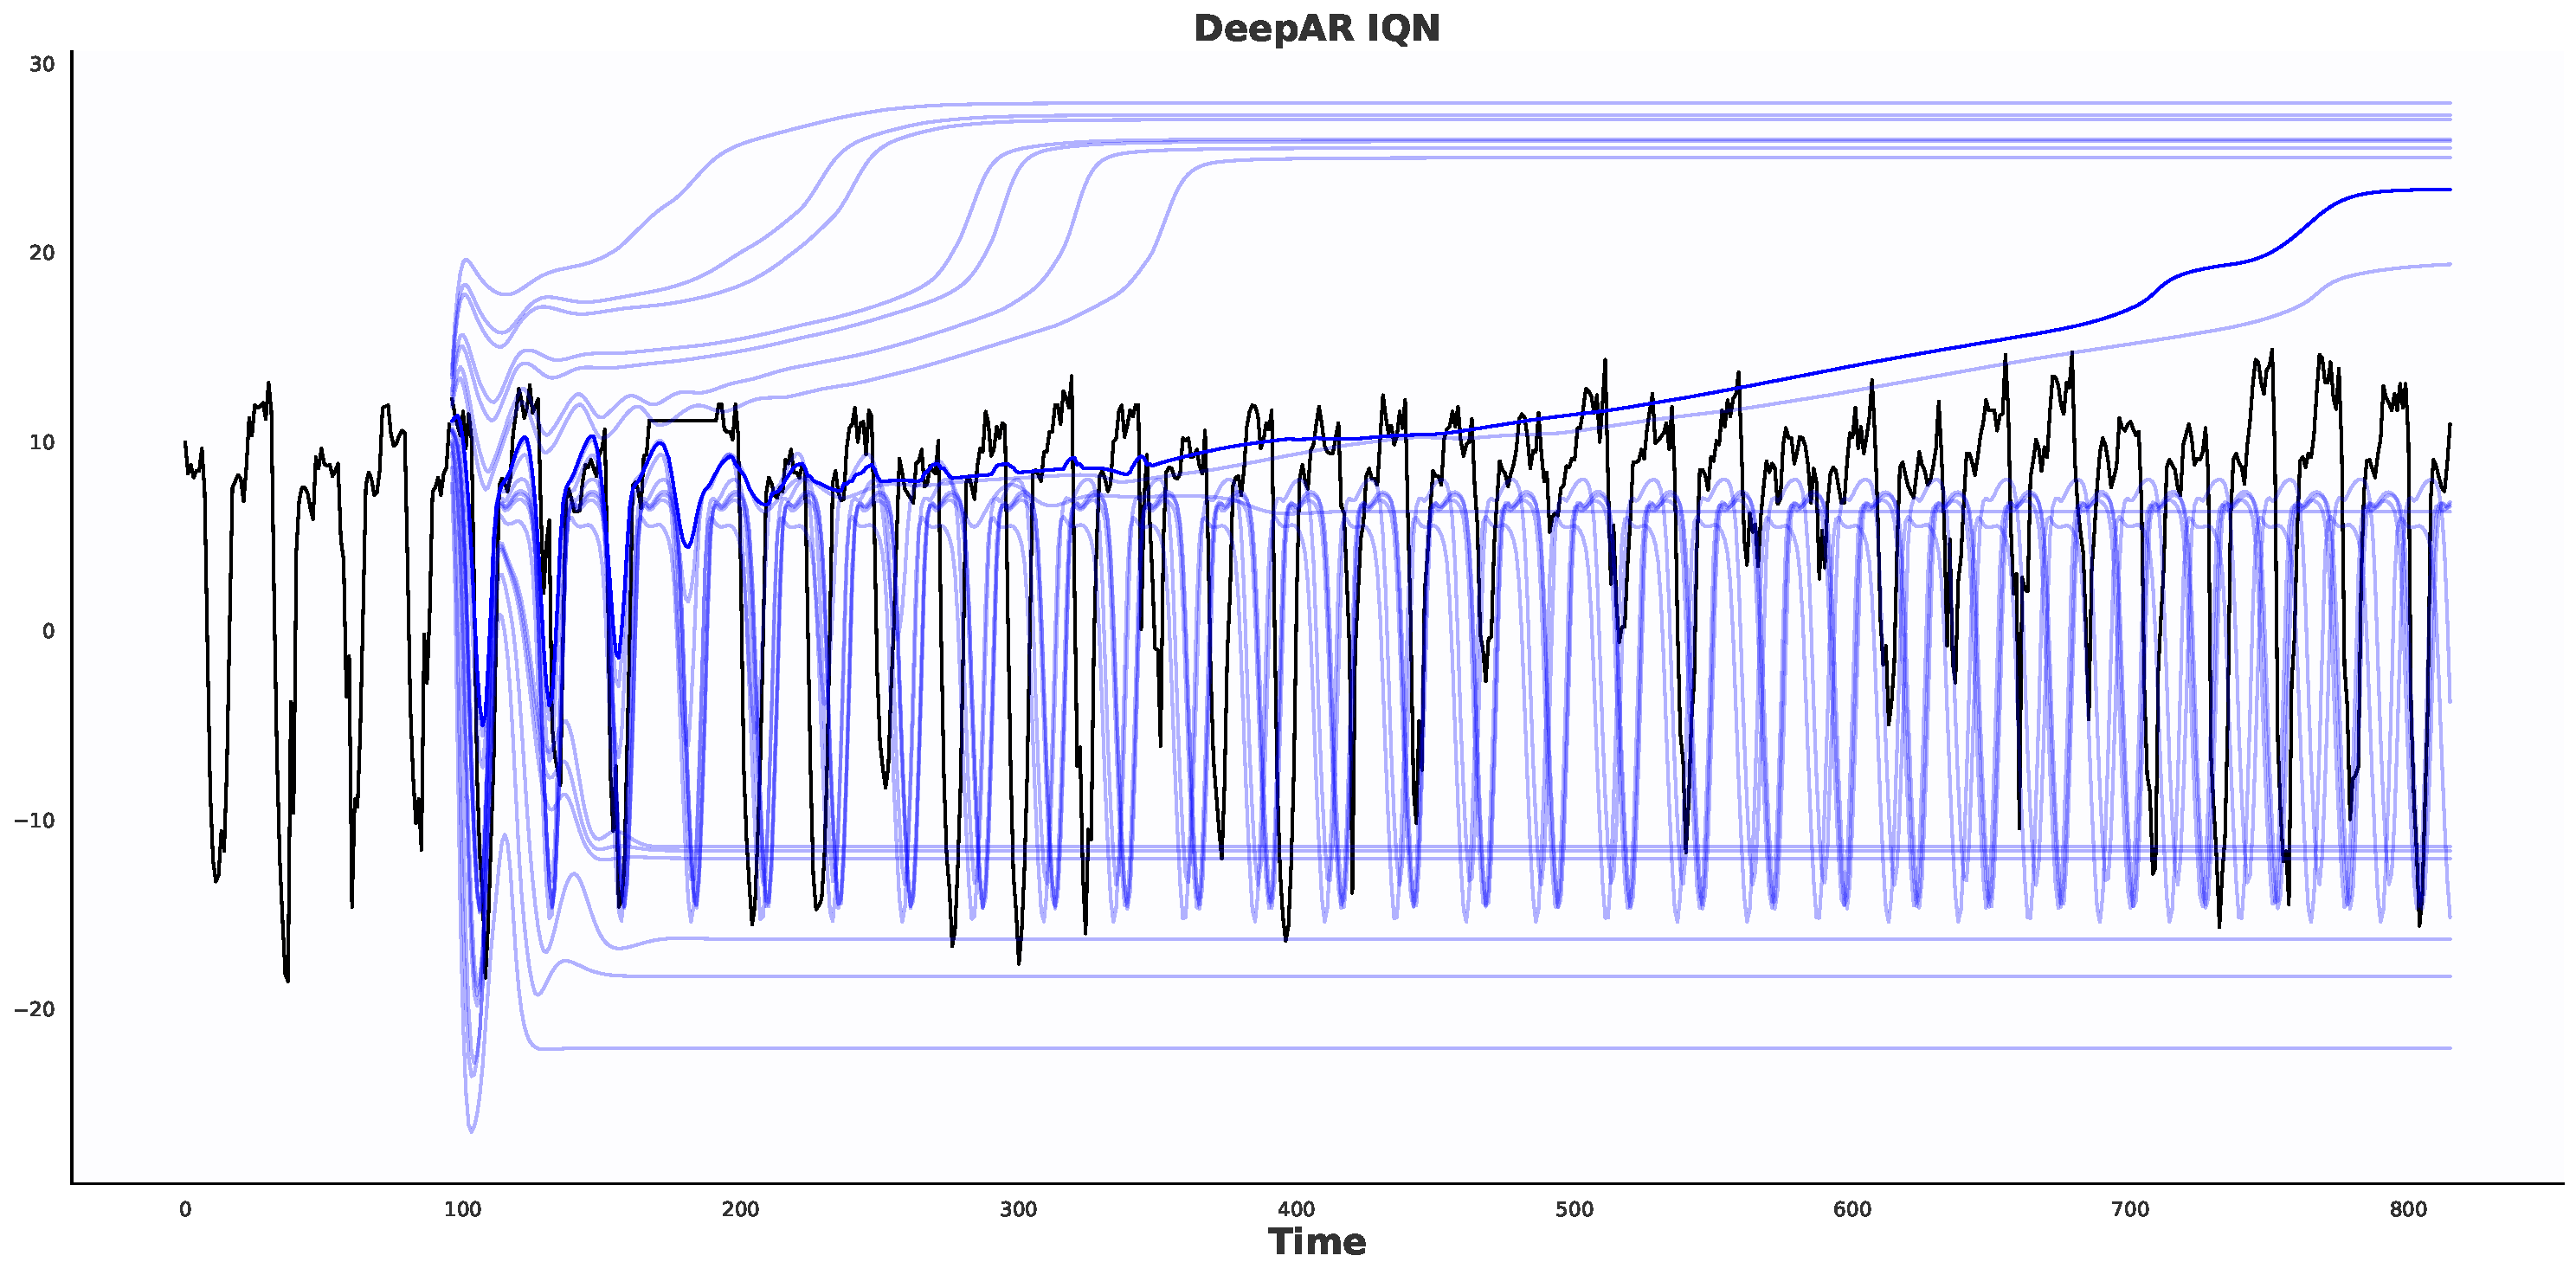
\includegraphics[width=\linewidth]{img/Experiments/ETTh1/fault_ims.pdf}
%     \caption{Visualization of the predictions of the IQN DeepAR model on ETTh1 with a constant quantile level for each trajectory. It becomes clear that the constant quantile level causes the model to diverge into unrealistic regions on many occasions.}
%     \label{fig:iqn_deepar_diverges}
% \end{figure}

% \begin{figure}[h]
% \centering
% \begin{minipage}{0.45\textwidth}
%   \centering
%   \includegraphics[angle=90, width=\linewidth]{img/Experiments/ETTh1/originals_samples_1.pdf}
%   \caption{20 sample forecasts per model for an instance of the LULL test time series, part of the ETTh1 dataset.}
%   \label{fig:ETTh1_samples}
% \end{minipage}
% \hfill
% \begin{minipage}{0.45\textwidth}
%   \centering
%   \includegraphics[angle=90, width=\linewidth]{img/Experiments/ETTh1/originals_samples.pdf}
%   \caption{20 sample forecasts for an instance of the HUFL test time series.}
%   \label{fig:ETTh1_samples_2}
% \end{minipage}
% \caption{Sample forecasts for two ETTh1 test time series. Each panel shows 20 forecast samples in blue and the corresponding ground truth in black. For the quantile-based methods, the "samples" shown correspond to the nine predicted quantile trajectories, as no sampling is performed in these cases.}
% \end{figure}

% \begin{figure}[h]
% \centering
% \begin{minipage}{0.45\textwidth}
%   \centering
%   \includegraphics[angle=90, width=\linewidth]{img/Experiments/ETTm1/originals_samples (5).pdf}
%   \caption{20 sample forecasts per method for an instance of the LULL test time series, part of the ETTm1 dataset.}
%   \label{fig:ETTm1_samples}
% \end{minipage}
% \hfill
% \begin{minipage}{0.45\textwidth}
%   \centering
%   \includegraphics[angle=90, width=\linewidth]{img/Experiments/ETTm1/originals_samples (7).pdf}
%   \caption{20 sample forecasts for an instance of the HUFL test time series.}
%   \label{fig:ETTm1_samples_2}
% \end{minipage}
% \caption{Sample forecasts for two ETTm1 test time series. Each panel shows 20 forecast samples in blue and the corresponding ground truth in black. For the quantile-based methods, the "samples" shown correspond to the nine predicted quantile trajectories, as no sampling is performed in these cases.}
% \end{figure}



% \begin{figure}
%     \centering
%     \includegraphics[width=\linewidth]{img/Experiments/ETTh1/Coverage_and_sharpness.pdf}
%     \caption{Calibration (left) and sharpness (right) curves for our probabilistic LTSF experiments on the ETTh1 data set, in which the single calibration plots aids in the comparison of inter-model differences.}
%     \label{fig:cov_sha_etth1_2}
% \end{figure}

% \begin{figure}
%     \centering
%     \includegraphics[width=\linewidth]{img/Experiments/ETTm1/Coverage_and_sharpness.pdf}
%     \caption{Calibration (left) and sharpness (right) curves for our probabilistic LTSF experiments on the ETTm1 data set, in which the single calibration plots aids in the comparison of inter-model differences.}
%     \label{fig:cov_sha_ettm1_2}
% \end{figure}


% % \citet{zobel2004} writes:

% % \blockcquote{zobel2004}{%
% %   Some papers have appendices giving detail of proofs or experimental results,
% %   and, where appropriate, material such as listings of computer programs. The
% %   purpose of an appendix is to hold bulky material that would otherwise
% %   interfere with the narrative flow of the paper, or material that even
% %   interested readers do not need to refer to. Appendices are rarely necessary.}

% % In the context of a BSc or MSc thesis, the last sentence often does not hold.

% \backmatter
% \chapter{Ehrenwörtliche Erklärung}

% Ich versichere, dass ich die beiliegende Bachelor-, Master-, Seminar-, oder
% Projektarbeit ohne Hilfe Dritter und ohne Benutzung anderer als der angegebenen
% Quellen und in der untenstehenden Tabelle angegebenen Hilfsmittel angefertigt
% und die den benutzten Quellen wörtlich oder inhaltlich entnommenen Stellen als
% solche kenntlich gemacht habe. Diese Arbeit hat in gleicher oder ähnlicher Form
% noch keiner Prüfungsbehörde vorgelegen. Ich bin mir bewusst, dass eine falsche
% Erklärung rechtliche Folgen haben wird.

% % Declare below which AI tools you used in the process of writing your work,
% % including text, image, code, and data generation. If you used a tool for a
% % purpose not included in the list yet, add it to the list.
% \begin{center}
%   \textbf{Declaration of Used AI Tools} \\[.3em]
%   \begin{tabularx}{\textwidth}{lXlc}
%     \toprule
%     Tool & Purpose & Where? & Useful? \\
%     \midrule
%     ChatGPT & Rephrasing & Throughout & + \\
%     DeepSeek & Rephrasing & Throughout & + \\
%     % ResearchGPT & Summarization of related work & Sec.~\ref{sec:related_work_A} & - \\
%     GPT-4 & Code generation & Codebase & + \\
%     Claude & Code generation & Codebase & + \\
%     \bottomrule
%   \end{tabularx}
% \end{center}

% \vspace{2cm}
% \noindent Unterschrift\\
% \noindent Mannheim, den 14.Juli 2025 \hfill

\end{document}
